%------------------------------------------------------------------------------
%
% OS 教科書
%
%------------------------------------------------------------------------------
\documentclass[a4paper,11pt,twocolumn]{ltjsbook}     % lualatex の場合
%----------- 印刷版とPDF版の区別 ----------------------------------------------
\newif\ifPDF
%印刷版の場合
%\PDFfalse
%PDF版の場合
\PDFtrue
\ifPDF
\newcommand{\pdf}{(PDF版)}
\else
\newcommand{\pdf}{}
\fi
%------------------------------------------------------------------------------
\usepackage{mySty}
\newcommand{\edition}{初版}
\newcommand{\ver}{Ver. 1.0.2}
\newcommand{\git}{https://github.com/tctsigemura/OSTextBook/tree/v1.0.0}
%\newcommand{\git}{https://github.com/tctsigemura/OSTextBook/blob/master}
%------------------------------------------------------------------------------
% はじまり
\begin{document}
%------------------------------------------------------------------------------
% カバー
\setcounter{page}{0}
\thispagestyle{empty}
\onecolumn
~
\vfill
\vfill
{\noindent
\fontsize{34pt}{50pt}\selectfont\textbf{オペレーティングシステム}\\
\fontsize{34pt}{50pt}\selectfont\textbf{Operating System}
}
\vfill
\vfill
\centerline{
  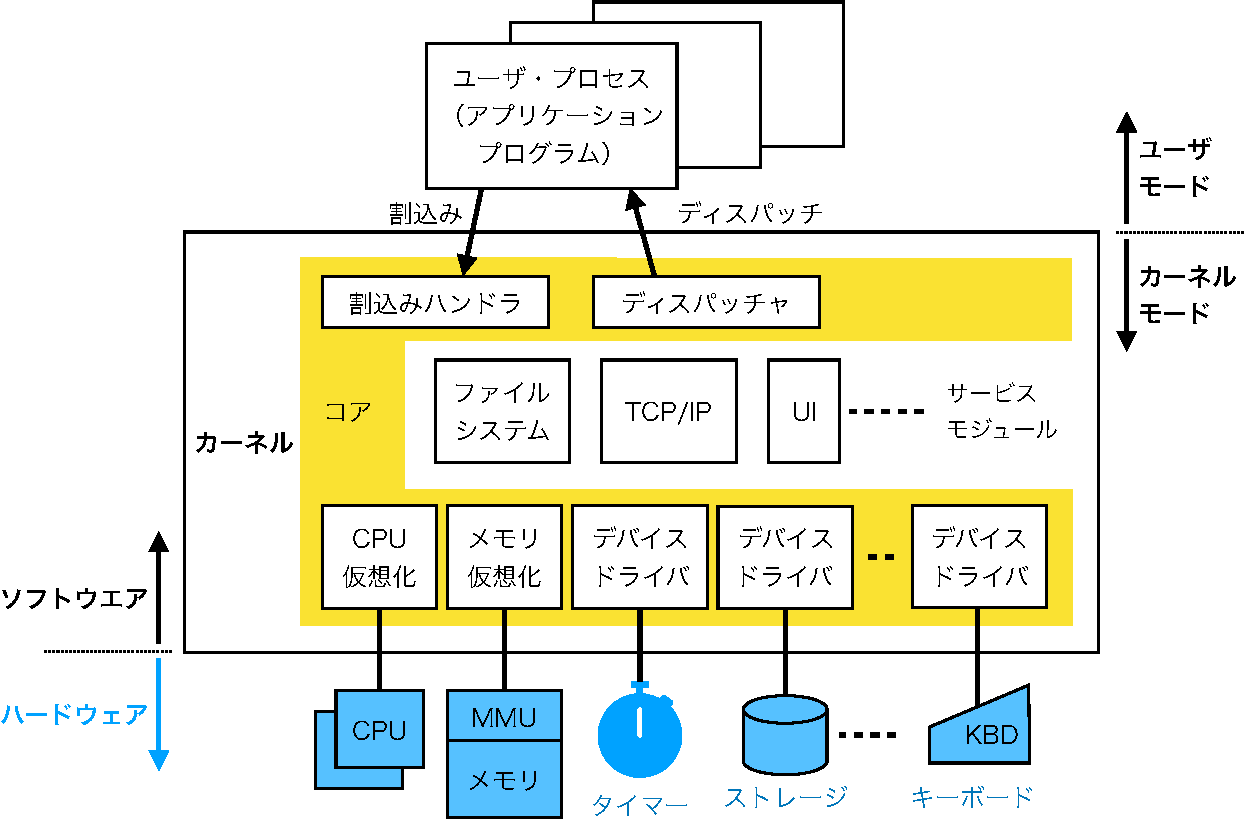
\includegraphics[scale=0.77]{Fig/osOrganization-crop.pdf}
}
\vfill
\vfill
\centerline{\Large 徳山工業高等専門学校 情報電子工学科}
%\centerline{\Large 重村研究室}
\centerline{\Large\ttfamily https://github.com/tctsigemura/OSTextBook/}
\vfill

%------------------------------------------------------------------------------
\ifPDF
\newpage
\setcounter{page}{0}
\thispagestyle{empty}
\onecolumn
~
\fi

%------------------------------------------------------------------------------
% 表紙
\frontmatter
\title{オペレーティングシステム{\pdf}\\{\edition}({\ver})}
\author{徳山工業高等専門学校\\情報電子工学科\\
\url{https://github.com/tctsigemura/OSTextBook/}}
\date{}
\maketitle

%------------------------------------------------------------------------------
% 著作権表示
\thispagestyle{empty}
\onecolumn
~
\vfill
\begin{flushleft}
Copyright \copyright ~~ 2018 by \\
Dept. of Computer Science and Electronic Engineering, \\
Tokuyama College of Technology, JAPAN
\end{flushleft}
\vspace{0.4cm}
\begin{flushleft}
本書は JSPS 科研費 22500833 および 16K0099 の助成を受けて作成しました.\\
本書はCC-BY-SA 4.0 ライセンスによって許諾されています。\\
本書の最新版は,以下からダウンロード可能です.\\
\url{https://github.com/tctsigemura/OSTextBook/blob/master/os.pdf}\\
本書の講義用スライドは,以下からダウンロード可能です.\\
\url{https://github.com/tctsigemura/OSTextBook/tree/master/Sld}
\end{flushleft}
\begin{flushleft}
本書はCC-BY-SA 3.0 de,CC-BY-SA 4.0 ライセンスで許諾された著作物を含みます.
\end{flushleft}
\begin{flushleft}
関係ライセンスの全文は,\\
 \url{https://creativecommons.org/licenses/by-sa/3.0/de/}
(CC-BY-SA 3.0 de),\\
 \url{https://creativecommons.org/licenses/by-sa/4.0/deed.ja}
(CC-BY-SA 4.0)\\
で確認できます.
\end{flushleft}
\begin{flushleft}
本書を授業などにご使用の節は,次のアドレスにご連絡いただければ幸いです.\\
sigemura@tokuyama.ac.jp
\end{flushleft}

%------------------------------------------------------------------------------
%目次
\setcounter{tocdepth}{1}
\tableofcontents

% 本文
\mainmatter

\part{OSとは}
\chapter{オペレーティングシステムとは}

オペレーティングシステム(Operating System : OS)は,
Windows,macOS,Linux,FreeBSD,Android,iOS
等である.
皆さんは,これらを使用した経験を持っているだろう.
そして,これらが次のようなソフトウェアから構成されていることを
何となく感じているのではないだろうか.

\begin{enumerate}
\item カーネル(OSの本体)
\item ライブラリ(プログラムが使用するサブルーチン,DLL)
\item ユーザインタフェース(GUI,CLI)
\item ユーティリティソフトウエア
  (ファイル操作,時計,シェル,システム管理 ...)
\item プログラム開発環境
  (エディタ,コンパイラ,アセンブラ,リンカ,インタプリタ)
\end{enumerate}

\emph{広義}では上に列挙した全て\footnote{
  上に挙げたソフトウェアの中で「プログラム開発環境」は,
  LinuxやFreeBSDではOSに含まれているが,
  それ以外では別にインストールする必要がありOSの一部とは言い難くなっている.
}がオペレーティングシステムの一部である.
逆に\emph{狭義}では「カーネル」だけをオペレーティングシステムと考える.
この講義では狭義のオペレーティングシステムの仕組みを勉強する.

%==============================================================================
\section{オペレーティングシステムの役割}
\label{osRole}

オペレーティングシステムの重要な役割は次に述べる二つである.

\subsection{拡張マシンとしてのオペレーティングシステム}
\label{abstruction}

OSはハードウェアの機能を\emph{抽象化}した便利な拡張マシンを提供する.
次に抽象化と拡張マシンの例を示す.

\begin{description}
\item[例1] 二次記憶装置の抽象化(ファイルシステム) \\
  ハードディスク,USBメモリ,CD-ROM等の二次記憶装置は,
  どれもデータを記録する機能を持ったハードウェアである.
  しかし,それらの制御方法や記録されるデータの構造は全く異なる.
  オペレーティングシステムは,
  二次記憶装置をファイルの集合(ファイルシステム)として\emph{抽象化}して
  ユーザプログラム(アプリケーションプログラム)に提供する.

\item[例2] コンピュータそのものの抽象化(プロセス) \\
  プロセスはプロセス専用の仮想CPUと仮想メモリを持つ.
  システムコールを通じて入出力も可能である.
  プロセスはCPU,メモリ,入出力を持っているので
  1台のコンピュータと考えることもできる.

  プロセスはコンピュータを\emph{抽象化}したものだとも言える.
  (プロセス=仮想コンピュータ)

\item[例3] 拡張されたコンピュータ(システムコール) \\
  オペレーティングシステムを備えたコンピュータ上では,
  アプリケーションプログラムがシステムコールを発行できる.
  システムコールを追加命令を考えると,
  オペレーティングシステムを備えたコンピュータは
  追加命令を実行可能な\emph{拡張マシン}だと言える.
  (拡張マシンの命令=機械語命令+システムコール)
\end{description}

オペレーティングシステムが
拡張マシンをアプリケーションプログラムに提供するイメージを
\figref{abstruction}に示す.
ハードウェアの複雑で統一されていない凸凹のインタフェースは,
オペレーティングシステムによってスッキリした円弧の
インタフェース(使いやすい\emph{抽象化}されたインタフェース)に変換される.

オペレーティングシステムの円がハードウェアの外側にあるのは,
オペレーティングシステムによって機能が拡張されたことを示す.
ハードウェアを含む円全体が拡張マシンを表している.

\begin{myfig}{btp}{抽象化}{abstruction}
  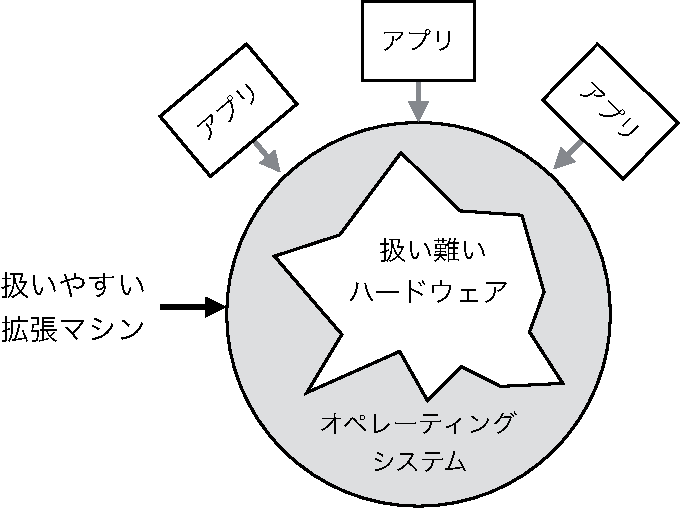
\includegraphics[scale=0.66]{Fig/abstruction-crop.pdf}
\end{myfig}

\subsection{ハードウェア管理プログラムとしてのオペレーティングシステム}
オペレーティングシステムはハードウェア資源を管理・制御し,
アプリケーションプログラムにシステムコール等のサービスを提供する.
\figref{system}はカーネルの役割を説明している.

オペレーティングシステムは,
管理するハードウェア資源をアプリケーションプログラムに割当てる.
複数のアプリケーションプログラムに割り付けるために
資源を\emph{仮想化}して必要な数だけ作り出す.
例えば,CPUは時間を区切って複数のプロセスが共有する
(\emph{時分割多重}による\emph{仮想化}).
メモリはアドレスで区切って複数のプロセスが共有する
(\emph{空間分割多重}による\emph{仮想化}).

\begin{myfig}{btp}{コンピュータシステムの構成}{system}
  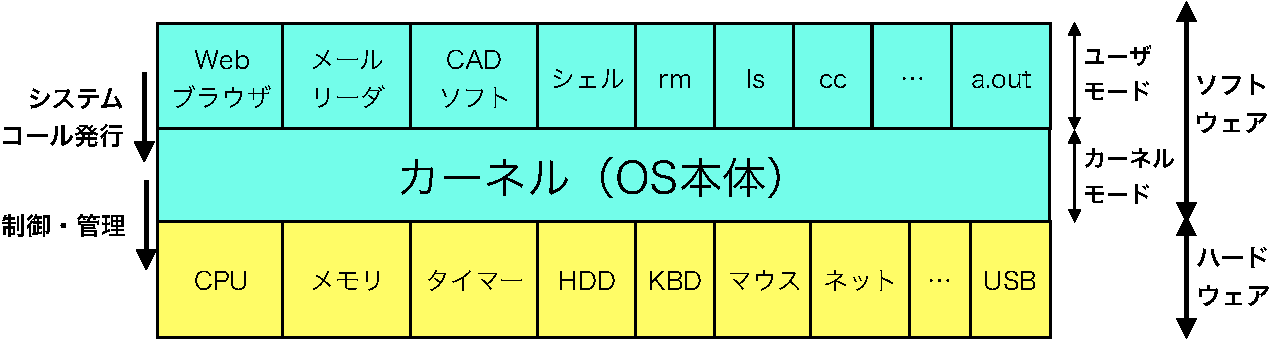
\includegraphics[scale=0.66]{Fig/system-crop.pdf}
\end{myfig}

%==============================================================================
\section{オペレーティングシステムの歴史}

\subsection{第1世代(1945〜1955,真空管の時代)}
初期のコンピュータはコンソールパネルを通して操作する,
巨大なTeC\cite{tec}のようなものだった.
OSは存在せずプログラマはまさにTeCと同様なプログラミングとデバッグを行っていた.

しかし,当時のコンピュータはTeCと異なり大変高価な装置であった.
その高価なコンピュータを一人のプログラマが長時間にわたって
独占使用することになる.
プログラマがバグの原因を考えている間,
とても高価なコンピュータが遊んでしまい勿体ないものであった.

\subsection{第2世代(1955〜1965,トランジスタの時代)}
\label{gen2nd}
コンピュータがトランジスタ回路で製作されるようになり,
\emph{メインフレーム}と呼ばれる大型コンピュータが,
大企業,政府機関や大学等で実用的に使用されるようになった.
メインフレームは数百万ドルと高価だったので,
ハードウェアを遊ばせること無く使用することが優先課題であった.
そこで人手を介すること無く自動的に次々と連続して処理を行う
「コンピュータの自動運転」が行われるようになった.
この処理方式のことは\emph{バッチ処理}と呼ばれた.
\figref{batch}にバッチ処理の概要を示す.

プログラマは\figref{punchcard}のような紙カードに
プログラムやデータを一行ずつ打込む.
100行のプログラムは100枚の紙カードを使用して記録する.
このようにして出来た紙カードの束が一つの処理単位(\emph{ジョブ})になる.
コンピュータでは\emph{バッチモニタ}と呼ばれる常駐プログラムが実行される.
バッチモニタは紙カードからジョブを読み込み実行させる.
ジョブが終了するとバッチモニタに制御が戻り次のジョブが自動的に実行される.
バッチモニタが発展してやがてOSになる.

\begin{myfig}{btp}{バッチ処理}{batch}
  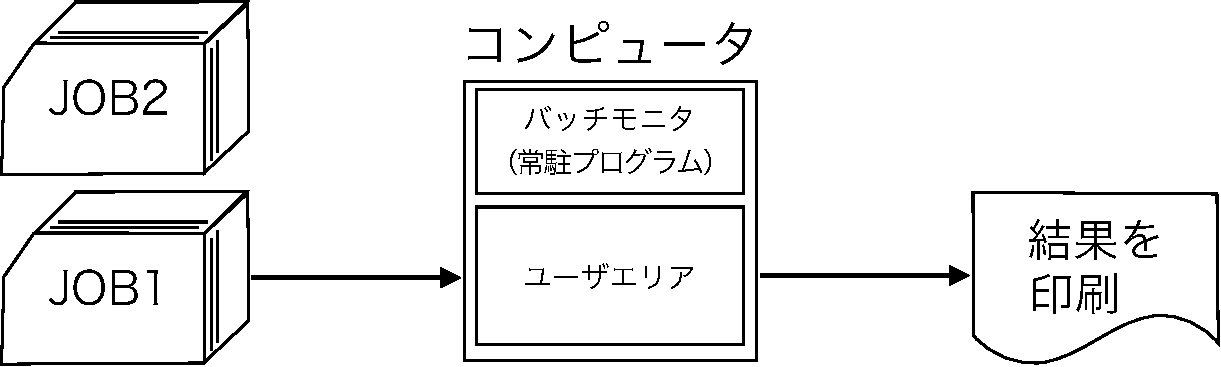
\includegraphics[scale=0.5]{Fig/batch-crop.pdf}
\end{myfig}

\begin{myfig}{btp}{紙カード}{punchcard}
  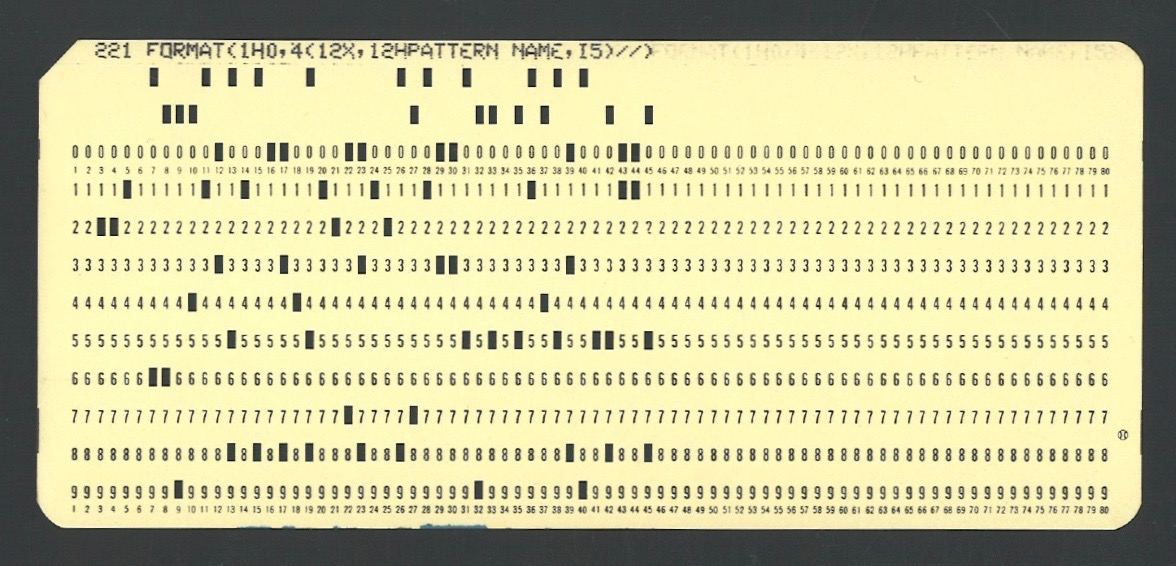
\includegraphics[scale=0.3]{Photo/punchcard.jpg}
\end{myfig}

この方式でうまく処理できるように,次のような発明があった.

\begin{enumerate}
\item \emph{JOB制御言語(JCL : Job Control Language)} \\
  バッチモニタを制御するコマンド言語をJOB制御言語(JCL)と呼ぶ.
  JCLコマンドはジョブ途中の紙カードに記載する.
  \figref{job}にJCLを含むジョブの構成を示す.
  これは,
  FORTRAN言語で記述したプログラムを実行し,
  後半にあるデータを処理するジョブの例になっている.

  \begin{myfig}{btp}{ジョブの構成}{job}
    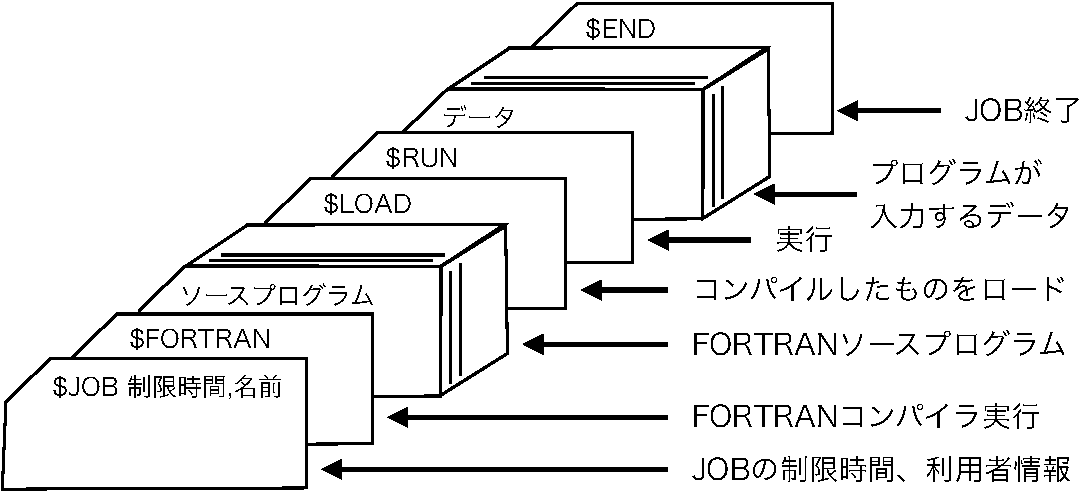
\includegraphics[scale=0.5]{Fig/job-crop.pdf}
  \end{myfig}

\item \emph{実行モード} \\
  ユーザプログラム(ジョブ)のバグで
  バッチモニタが破壊されないようにするために,
  ユーザプログラム実行中なのかバッチモニタ実行中なのか区別する必要がある.
  どちらを実行中なのかを示すハードウェアのフラグを導入し,
  \emph{ユーザモード}と
  \emph{カールモード}(\emph{スーパバイザモード}とも呼ぶ)を
  区別するようになった.
  ユーザモードではハードウェアへのアクセスや,
  実行できる機械語命令に制限がある.

\item \emph{システムコール} \\
  ユーザプログラムが直接に入出力装置等にアクセスすることは,
  バッチ処理を継続できなくする恐れがあるので許されない.
  例えばユーザプログラムがハードウェアのモードを切り換えてしまうと,
  以降のジョブが正常に実行されなくなる恐れがある.
  そこで,ユーザプログラムはバッチモニタに依頼(システムコール)して
  入出力を行う必要がある.

  プログラムが終了する時は
  カーネルモードに切り換えてバッチモニタに戻る必要がある.
  カーネルモードに切り替える機械語命令をユーザプログラムが実行可能だと,
  実行モードが無意味になるので許可すべきではない.
  システムコールを使用してプログラムを終了する.

\item \emph{記憶保護} \\
  ユーザプログラムのバグでバッチモニタが破壊されないように,
  ユーザモードで実行中は
  主記憶のバッチモニタ領域に書込みができないようにする.
\end{enumerate}

\subsection{第3世代(1966〜1980,ICとマルチプログラミングの時代)}
1960年代のコンピュータはIC(Integrated Circuit)を用いて作られるようになり
価格性能比が随分改善された.
第3世代と呼ばれる当時のオペレーティングシステムの中には,
現代のオペレーティングシステムの先祖であったり,
強い影響を与えたものがある.
\figref{tree}に第3世代から現代に至るまでの系統図を示す.


IBMが開発したSystem/360(\figref{system360})は高価な大型のものから,
安価な小型のものまでで同じオペレーティングシステムが使用でき,
同じユーザプログラムを実行できる\emph{シリーズ化}を行い商業的に大成功をおさめた
\cite{third}.
System/360はそれ以前のものとは異なり科学技術計算にも事務処理にも使用できる.
System/360のオペレーティングシステムは,
1966年にデビューしたOS/360である.
\figref{tree}に示すように,
OS/360の子孫であるz/OSが現代でも使用されている\cite{os360}.

\begin{myfig}{btp}{フォルクスワーゲンで使われているSystem/360}{system360}
  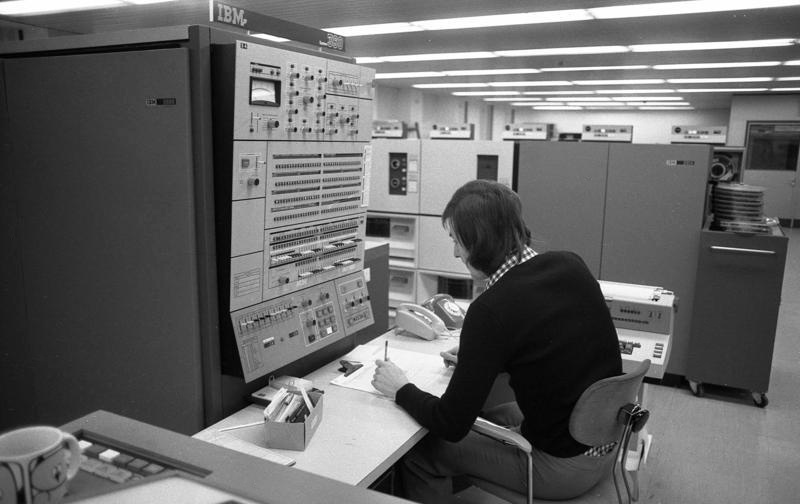
\includegraphics[scale=0.25]
  {Photo/Bundesarchiv_B_145_Bild-F038812-0014,_Wolfsburg,_VW_Autowerk.jpg}\\
  {\small
    ウィキメディア /
    Bundesarchiv, B 145 Bild-F038812-0014 /
    Schaack, Lothar / CC-BY-SA 3.0 de}
\end{myfig}

OS/360を含む第3世代のオペレーティングシステムが
実現した重要な新しい機能を紹介する.

\begin{itemize}
\item \emph{仮想記憶} \\
  主記憶を仮想化し実際より大きい主記憶があるように見せる.
  実際の主記憶より大きいプログラムが実行可能になる.

\item \emph{マルチプログラミング} \\
  \label{multiprogramming}
  \figref{multiprogramming}のように,
  複数のプログラム(ジョブ)を主記憶にロードしておき,
  その中で実行可能なものを選んで実行する.
  入出力待ち等で実行できなくなったら他のプログラムを実行する.
  高価なCPUが入出力待ちで停止する可能性を低くすることができた.

  \begin{myfig}{btp}{マルチプログラミングシステム}{multiprogramming}
    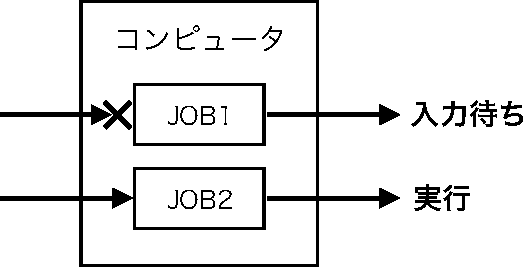
\includegraphics[scale=0.66]{Fig/multiprogramming-crop.pdf}
  \end{myfig}

\item \emph{タイムシェアリング(TSS:Time Sharing System)} \\
  マルチプログラミングの一種である.
  \figref{timesharing}のように,
  複数のターミナルをコンピュータに接続し
  複数のユーザが同時にコンピュータを使用できるようにする.
  短時間(例えば10ms)で処理するジョブを次々に切り換えることで,
  ユーザは自分がコンピュータを独占しているように感じることができる.
  なお,ターミナルは\figref{terminal}のような,
  キーボードと表示装置だけを備えた安価な装置である.

  \begin{myfig}{btp}{タイムシェアリングシステム}{timesharing}
    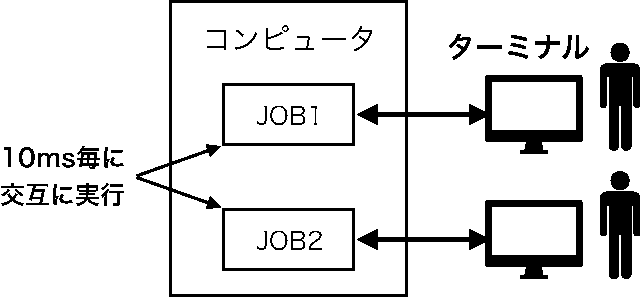
\includegraphics[scale=0.66]{Fig/timesharing-crop.pdf}
  \end{myfig}

  \begin{myfig}{btp}{ターミナル}{terminal}
    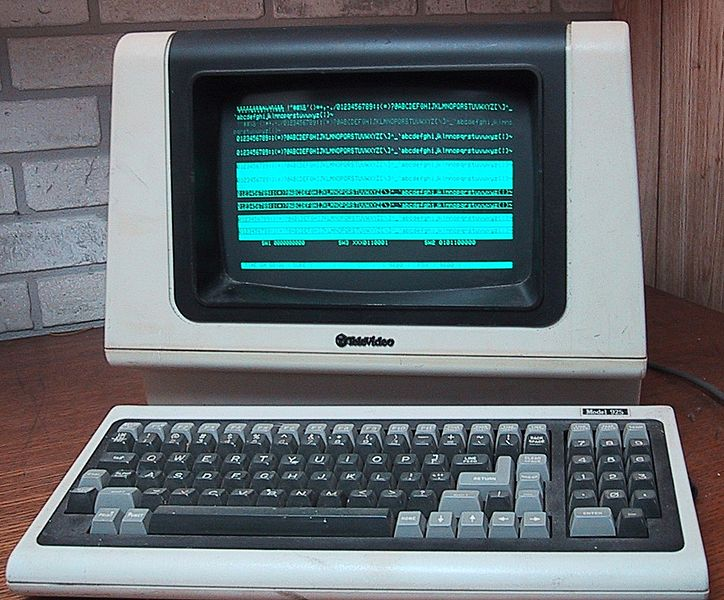
\includegraphics[scale=0.25]
     {Photo/724px-Televideo925Terminal.jpeg}\\
     {\small 写真:
       \url{http://commons.wikimedia.org/wiki/File:Televideo925Terminal.jpg}
       (パブリックドメイン)}
  \end{myfig}
\end{itemize}

この時代のオペレーティングシステムやコンピュータシステム,
そして,それらの開発プロジェクトの中で,
その後のオペレーティングシステムに多くの影響を与えた有名なものを紹介する.

\begin{itemize}
\item OS/360 \\
  世界初の本格的な商用オペレーティングシステムである.
  メインフレームの主流OSとなり子孫は現在でも使用されている\cite{os360}.

\item MULTICS(MULTiplexed Information and Computing Service)プロジェクト
  \cite{third} \\
  MIT,ベル研究所,General Electricが共同で始めた
  巨大で強力なコンピュータシステムを構築するプロジェクトである.
  強力な一台のコンピュータで
  都市一つ分のコンピュータサービスを提供する構想だった.
  完成までに長い期間を要し(その間にベルとGEが脱落し),
  商業的には失敗であったがその後のオペレーティングシステムに影響を与える
  多くのアイデアが出てきた.

\item UNIX(ユニックス) \\
  MULTICSプロジェクトから抜けたベル研のKen Thompsonらにより開発された
  \cite{unix}.
  \figref{tree}に示すように,
  現代のオペレーティングシステムの多くがUNIXを起源にしている.
  子孫ではないものもUNIXの影響を強く受けている.
  LinuxはUNIX互換のオペレーティングシステムを作ろうとして
  開発が始まった\cite{linux}.
  Androidの中身はLinuxである\cite{android}.
  z/OSはUNIX互換環境を備えている\cite{zos}.
  WindowsにもUNIX互換環境(POSIXサブシステム)を
  利用可能なものがある\cite{windows}.

\item DynaBook(ダイナブック:OSだけでなくコンピュータ全体を指す)
  \cite{dynabook2} \\
  アラン・ケイが1972年に著した
  「A Personal Computer for Children of All Ages」\cite{key72, key72J}
  に登場する理想のパーソナルコンピュータである.
  アラン・ケイがゼロックスのパロアルト研究所に在籍中の1970年代に開発した
  Alto上の「暫定ダイナブック環境」(\figref{smalltalk})は
  既にGUIやマウスを使用していた.
  スティーブ・ジョブスがAltoを見たことが
  LISA開発きっかけになったと言われている\cite{dynabook}.

  \begin{myfig}{btp}
    {Alto(Alto エミュレータ)のスクリーンショット}
    {smalltalk}
    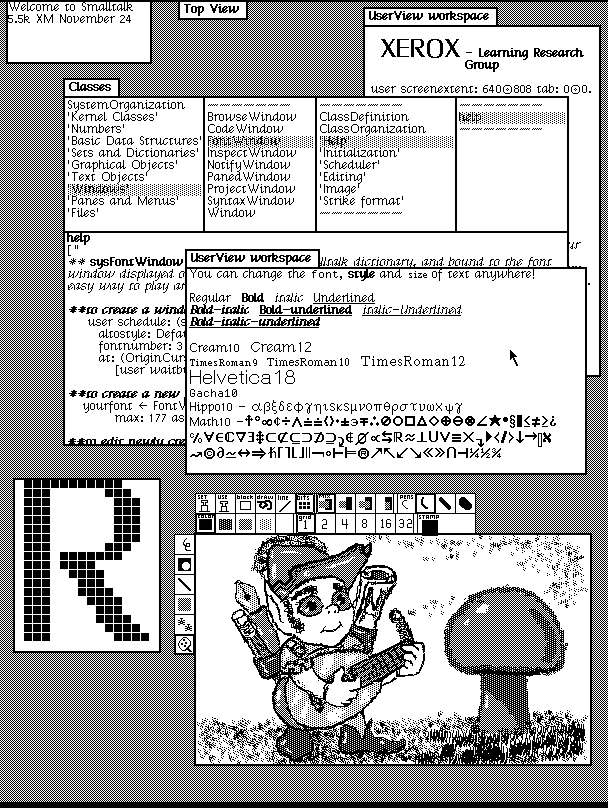
\includegraphics[scale=0.5]{Photo/Smalltalk-76.png}\\
                    {\small
                      ウィキメディア /
                      SUMIM.ST /\\
                      AltoやNoteTakerで動作した
                      アラン・ケイ達の暫定Dynabook環境
                      (Smalltalk-76、同-78の頃) /
                      CC-BY-SA 4.0
                    }
  \end{myfig}

\end{itemize}

\subsection{第4世代(1980〜現代,PCの時代)}

1970年代に単一のLSIにCPU全体を集積したマイクロプロセッサが登場した.
1970年代中頃にはマイクロプロセッサを用いて個人向けのコンピュータである
パーソナルコンピュータ(当時はマイクロコンピュータと呼んでいた)
を作ることが可能になった.
それに伴いパーソナルコンピュータ用のオペレーティングシステムが登場した.

\begin{enumerate}
\item 8bitマイクロコンピュータの時代 \\
  1977年にDigtal Reserch社がCP/M(Control Program for Microcomputer)と呼ばれる
    8bitマイクロコンピュータ用の簡単なオペレーティングシステムを
    開発し成功した.
    しかしこのオペレーティングは16bitパーソナルコンピュータの時代には
    早々に消え去ってしまった\cite{fourth}.

  \item 16bitパーソナルコンピュータの時代 \\
    IBMが1981年に16bitパーソナルコンピュータIBM PC\cite{ibmpc81}
    (\figref{ibmpc})を発売した.
    IBM PCは現在のWindows PCの先祖である.
    IBM PCの子孫は改良や拡張を続けながら現在まで高いシェアを維持し続けている.
    IBM PCのオペレーティングシステムとして開発されたのが,
    Microsoft社のMS-DOS(MicroSoft Disk Operating System)\cite{msdos}である.
    バージョン2からはUNIXのような
    階層ディレクトリやパイプ,リダイレクト等の機能を持っている.
    \figref{tree}に示すように,MS-DOSはWindowsに置き換わりWindows MEまで
    バージョンアップが繰り返された.

    \begin{myfig}{btp}{IBM PC}{ibmpc}
      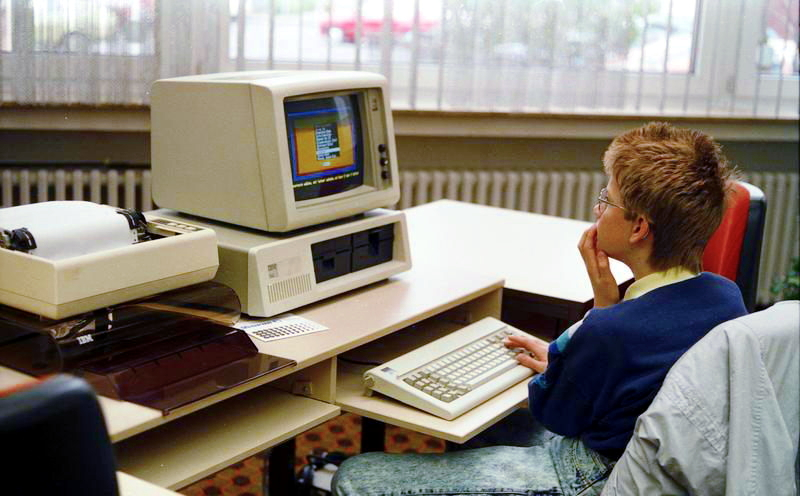
\includegraphics[scale=0.35]
                      {Photo/Bundesarchiv_B_145_Bild-F077948-0006,_Jugend-Computerschule_mit_IBM-PC.jpg}\\
                      {\small
                        ウィキメディア /
                        Bundesarchiv, B 145 Bild-F077948-0006 /
                        Engelbert Reineke / CC-BY-SA 3.0 de}
    \end{myfig}

    Apple社は1984年にMacintosh(\figref{macintosh})を発売した.
    MachintoshのOSであるMacOSはLISAを経てDynaBook\cite{key72, key72J}の
    影響を受けていると言われている\cite{fourth}.
    \figref{tree}に示すように,
    当初のMacOSはMacOS 9\cite{classicmacos}まで改良が続けられた.

    \begin{myfig}{btp}{初代Macintosh}{macintosh}
      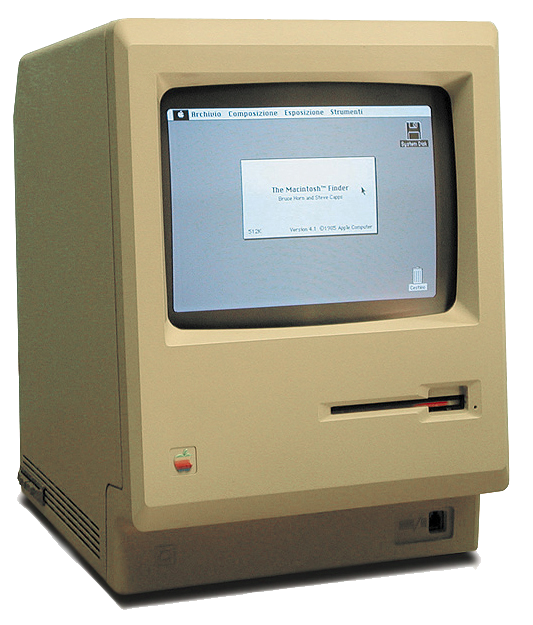
\includegraphics[scale=0.25]{Photo/Macintosh_128k_transparency.png}\\
                      {\small
                        ウィキメディア / w:User:Grm wnr /
                        File:Macintosh 128k transparency.png /GFDL}
    \end{myfig}

  \item 32bitパーソナルコンピュータの時代 \\
    1990年頃には32bitのマイクロプロセッサが
    パーソナルコンピュータにも使用されるようになった.
    32bitのマイクロプロセッサは実行モードを備え,
    またメモリ管理ユニットも利用可能であった.
    つまり,カーネルモードとユーザモードを使い分けたり
    仮想記憶を利用する本格的な第3世代のオペレーティングシステムを
    実行できる環境がパーソナルコンピュータにも整った.

    そこで,
    従来ワークステーションやミニコンで使用されていた
    UNIXを安価なパーソナルコンピュータ(特にIBM PC互換機)で
    動くようにする人たちが現れ,
    オープンソースソフトウェアとしてLinuxやFreeBSD等の開発が始まった.
    また,もともとパーソナルコンピュータ用のWindowsやMacOSも
    32bitマイクロプロセッサの機能を使いこなす
    本格的なオペレーティングシステムに生まれ変わった.

    \begin{itemize}
    \item Linux \\
      1991年に開発が始まったLinuxはUNIX互換のオペレーティングシステムを
      パーソナルコンピュータ(IBM PC互換機)用に
      独自に作成したものである\cite{linux}.
      Linuxは改良され続け,
      現在ではパーソナルコンピュータだけでなく,
      スーパーコンピュータ「京」のオペレーティングシステム\cite{kei}から,
      スマートフォンのオペレーティングシステムであるAndroid\cite{android},
      テレビ等の組込みシステムのオペレーティングシステムまで,
      広く使われるようになっている.

    \item BSD 系の UNIX \\
      386BSD\cite{386bsd}はBSD UNIXをIntel 80386 CPUを搭載した
      パーソナルコンピュータ(IBM PC互換機)で動作するようにしたものである.
      386BSDはFreeBSD等に受継がれるがUNIXのライセンス問題が発生する\cite{unix}.
      ライセンス問題が片付き安心して使用できるようになった
      4.4BSD-Lite Release 2\cite{unix}をベースに
      FreeBSD, NetBSD, OpenBSD 等の多くの BSD 系 PC-UNIXが開発された.

      その後,FreeBSDは MacOS X に取り込まれている.
      また,FreeBSDにZFSが移植された\cite{zfs}ので
      ファイルサーバ用に特化したFreeNAS\cite{freenas}にも使用されている.
      なお,徳山工業高等専門学校・情報電子工学科のパソコン室では
      1993年10月に386BSDの利用を開始して以来,
      2014年3月までFreeBSDを学生用PCやサーバのオペレーティングシステムとして
      使用してきた\cite{iebsd}.

    \item System V 系の UNIX \\
      System V の流れを汲むSolaris\cite{solaris}は,
      RISC マイクロプロセッサ SPARC を搭載するサーバやワークステーションでも,
      パーソナルコンピュータ(IBM PC 互換)でも使用できる.

    \item 従来のパーソナルコンピュータ用オペレーティングシステム \\
      従来のWindowsやMacOSはCPUの実行モード等を使用していなかったので,
      アプリケーションプログラムのバグにより
      システム全体が停止するようなトラブルを防ぐことができなかった.
      そこで,32bitマイクロプロセッサの使用を前提に新しく作り直された.

      新しく作り直された32bitのWindows NT系列の製品は,
      徐々に従来のWindowsを置換えた.
      (\figref{tree}参照).
      現在(2017年10月)の最新版はWindows 10である.

      MacOS は,2001年にUNIXの流れを汲み安定して動作するOPENSTEPベースの
      MacOS X\cite{macos}に置き換わった(\figref{tree}参照).
      その後,名称が OS X, macOS と変更されたがこれらは MacOS X の改良版である.
      現在(2017年10月)の最新版はmacOS 10.13 High Sierraである.
      iPhoneのiOSはMacOS Xをタッチパネル用に再構成したものである\cite{ios}.
    \end{itemize}
\end{enumerate}

\subsection{インターネット世代}
現在のオペレーティングシステムはTCP/IP機構が組込まれ
インターネットに接続することができる.
今ではパーソナルコンピュータやスマートフォンの使用を
インターネット抜きに考えることができない.
オペレーティングシステムにとってインターネットに接続できることは
重要なことである.

TCP/IPを実装した4.2BSDが1984年に公開された\cite{bsd}.
以来,4.2BSDの子孫はインターネットに対応している.
1988年に公開されたSystem V R4はBSD起原のTCP/IPの実装を含んでいた\cite{svr4}.
これの子孫もインターネットに対応している.
Linuxも1.0の頃にはTCP/IPの実装を含んでいた\cite{linux1}.
WindowsはWindows 95からTCP/IPを標準装備している\cite{windows}.
MacOSはMacOS 8が発表されるまでにはインターネット対応がされていた
\cite{classicmacos}.
メインフレームの世界でもOS/390はインターネットに対応した\cite{os390}.

このようにして1990年代の後半には多くのオペレーティングシステムが
インターネット対応を完了させた.
インターネット対応を完了させたオペレーティングシステムを
「インターネット世代のオペレーティングシステム」と言うことができる.

\begin{myfig}{btp}{オペレーティングシステムの系統図}{tree}
  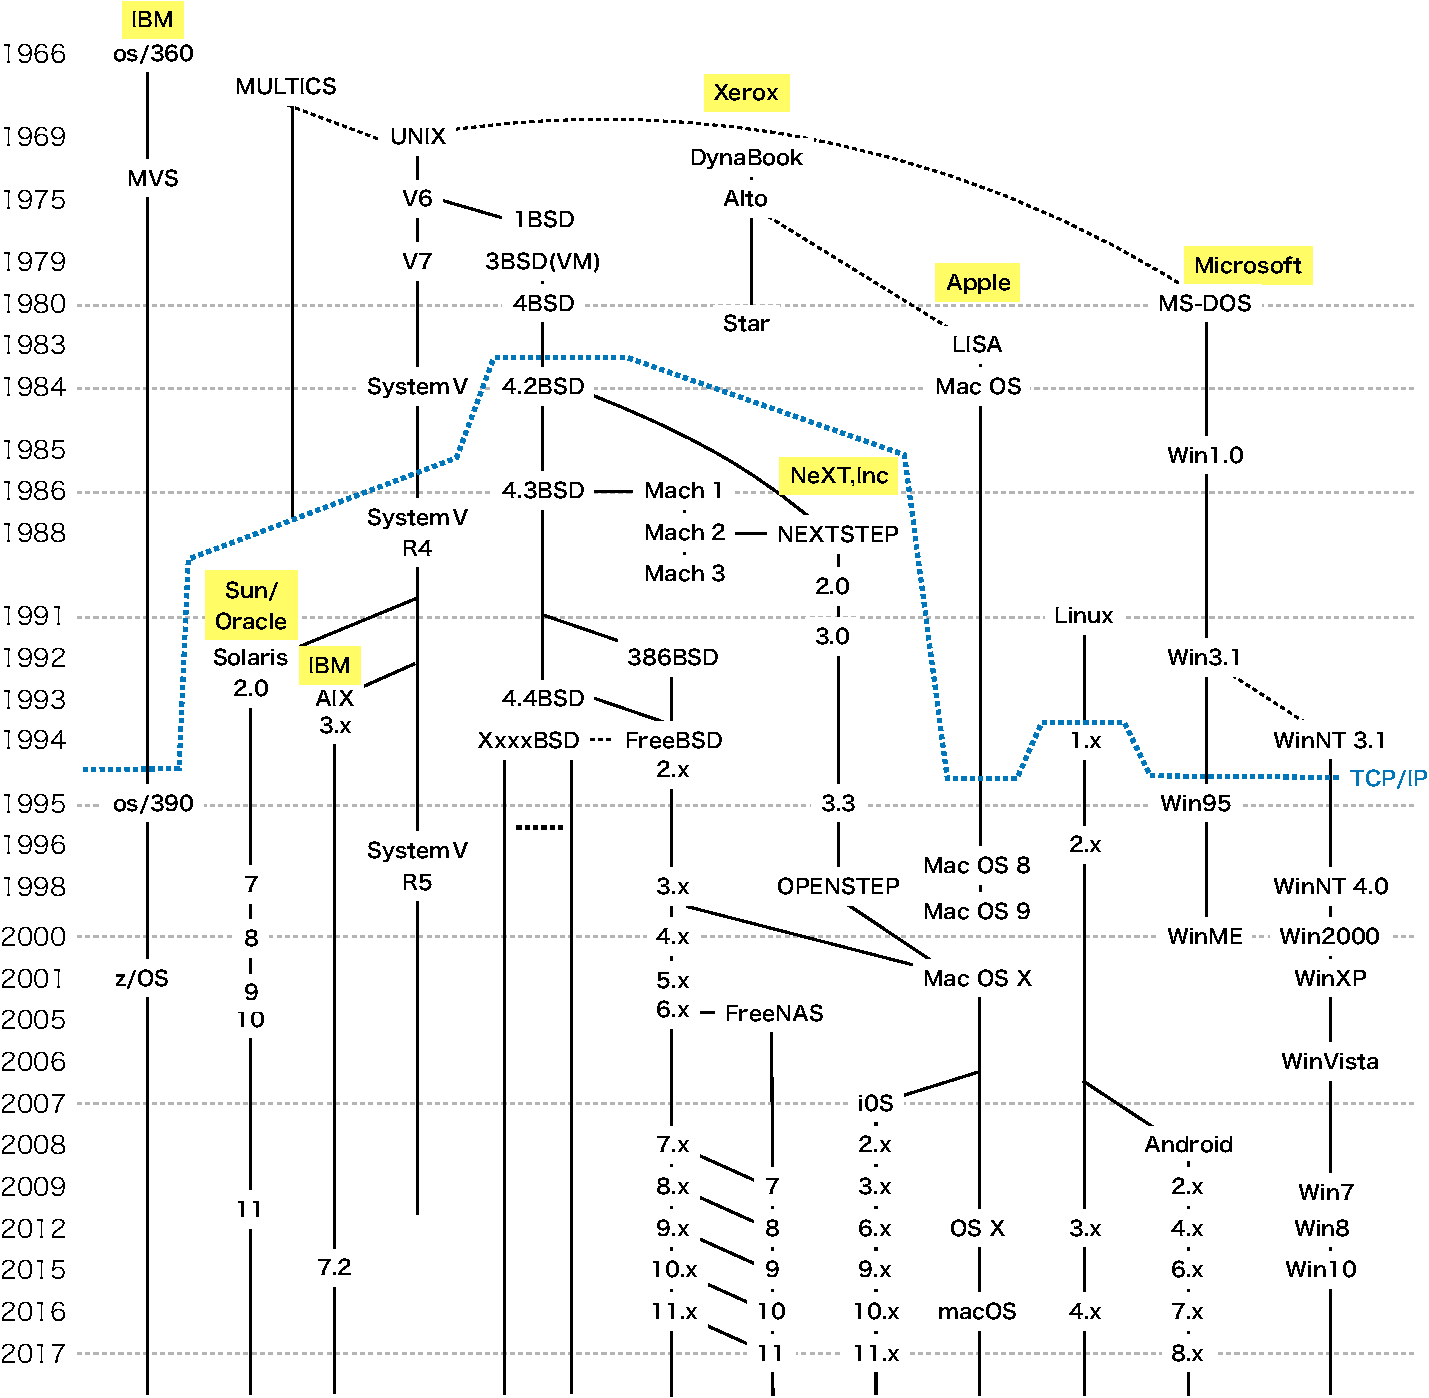
\includegraphics[scale=0.6]{Fig/tree-crop.pdf}\\
                  {\small
                    系統図は\cite{os360,
                      mvs,
                      os390,
                      zos,
                      unix,
                      solaris,
                      aix,
                      mach,
                      bsd,
                      bsdd,
                      386bsd,
                      freebsd,
                      freenas,
                      nextstep,
                      classicmacos,
                      dynabook,
                      macos,
                      ios,
                      linux,
                      android,
                      msdos,
                      windows}
                    の内容を総合して作成した.}
\end{myfig}

%==============================================================================
\section{まとめ}
狭義のオペレーティングシステムは\emph{カーネル}のことを指す.
本書は狭義のオペレーティングシステムについて述べている.

オペレーティングシステムの重要な役割りは,
コンピュータの資源を\emph{抽象化}することと\emph{仮想化}することである.
オペレーティングのユーザは,
使いやすい抽象化されたインタフェースを通して資源を利用できる.
また,ユーサは仮想化された資源を必要なだけ独占して使用することができる.

オペレーティングシステムは,
1950年代に出現したバッチモニタから進化してきた.
現在では,
スーパーコンピュータから組み込み用コンピュータまで,
非常に広い範囲のコンピュータが本格的なオペレーティングシステムを搭載している.


%==============================================================================
\section*{練習問題}
\begin{enumerate}
  \renewcommand{\labelenumi}{\ttfamily\arabic{chapter}.\arabic{enumi}}
  \setlength{\leftskip}{1em}
\item \emph{抽象化}について説明しなさい.
\item \emph{抽象化}の例をいくつか挙げなさい.
\item \emph{仮想化}について説明しなさい.
\item \emph{仮想化}の例をいくつか挙げなさい.
\item 自分がいつも使用しているコンピュータやスマートフォンの
  オペレーティングシステムの種類を調べなさい.
\end{enumerate}
 % オペレーティングシステムとは
\chapter{前提知識}
以下では,
本書で想定しているコンピュータのハードウェアやソフトウェアの
構成について解説する.

\section{コンピュータのハードウェア構成}
本書は,
コンピュータのハードウェア構成が\figref{hardBlock}のようになっている
ことを前提にしている.
複数のCPU(Central Processing Unit)がメモリを共有し,
また,全てのCPUは同じ機能を持ち優劣が無い.
このような方式を
{\bf SMP(対称型マルチプロセッシング:Symmetric Multiprocessing)}と呼ぶ.
メモリはCPUだけでなく,
I/Oコントローラ(\figref{hardBlock}ではアダプタやコントローラ)にも
共有される.

\myfigure{btp}{scale=0.48}{Fig/hardBlock-crop.pdf}{ハードウエア構成}{hardBlock}

\begin{enumerate}
\item CPU \\
CPUはコンピュータの頭脳である.
図はCPUが二つの構成になっているが,
実際は一つの場合も,もっと多い場合もある.

\item メモリ(主記憶装置) \\
プログラムやデータを記憶し,
プログラム実行する際にCPUが直接使用する記憶装置である.

\item タイマー \\
一定間隔で繰り返しCPUに割り込みを発生するインターバルタイマーである.

\item グラフィックアダプタ \\
ディスプレイを接続するためのアダプタである.
表示内容を記憶するメモリを独自に持つ場合と,
主記憶装置を使用する場合がある.
最近のパーソナルコンピュータでは,
グラフィックアダプタにGPU(Graphics Processing Unit)が組込まれている.

\item SATA ホストコントローラ \\
SATA(Serial Advanced Technology Attachment)は,
パーソナルコンピュータと二次記憶装置(ハードディスクやCD-ROM)を接続するための
インタフェース規格である.
SATA ホストコントローラは次のような動作をする.
\begin{enumerate}
\item CPUがSATAホストコントローラにコマンドを書き込む.
コマンドは,
「読み/書き」,「セクタアドレス」,「セクタ数」,「メモリアドレス」
を含んだものである.
\item SATAホストコントローラは,
ディスクコントローラと通信しハードディスクにコマンドを渡す.
\item ハードディスクの読み・書きが可能になったら,
ホストコントローラはハードディスクとメモリの間でデータ転送を行う.
このようなCPUを介さないデータ転送のことを,
{\bf DMA(Direct Memory Access)}と呼ぶ.
\item SATAホストコントローラはCPUに割り込み信号を送り,
データの転送が完了したことを知らせる.({\bf I/O完了割り込み})
\end{enumerate}
CPUは,
SATAホストコントローラにコマンドを送ってから割り込みが発生するまでの間,
他の仕事をすることができる.
ハードディスクの操作(I/O操作)とCPUの計算は並列実行される.

\item USBコントローラ \\
USB(Universal Serial Bus)は,
パーソナルコンピュータと周辺装置を手軽に接続できるインタフェースである.
USBメモリスティックやプリンタ,キーボード,マウス等,多くの周辺装置が
USBを通して接続できる.
USBコントローラもSATAホストコントローラのようにDMA機能を備えている.

\item ネットワークアダプタ \\
パーソナルコンピュータのネットワークアダプタは,
GbE(Gigabit Ethernet)規格のものが普及している.
これもSATAホストコントローラのようにDMA機能を備えている.

\item BUS(バス) \\
パーソナルコンピュータのハードウェアを構成する装置の間で
データをやり取りするための配線である.
CPUだけでなくDMAを使用するコントローラやアダプタが大量のデータ転送を行うので,
バスのデータ転送能力がパーソナルコンピュータの性能向上のボトルネックになる.

そのため後で説明するように,実際の物理的な接続は\figref{hardBlock}とは
かなり異なった構成になっている.
しかし,オペレーティングシステムが意識しなければならない論理的な
接続は\figref{hardBlock}のようなものである.

\end{enumerate}

\section{CPUの構成}
本書では、CPUは\figref{cpuBlock}のような部品で構成されると考える.
\figref{hardBlock}に示したように,CPUはBUSを通して他の装置と接続される.
CPUは,一つの機械語命令の実行が終わり次の命令の実行を開始する前に,
他の装置から割り込みを受け付けることができる\footnote{
例外的に,メモリ管理に関する一部の割込は機械語命令の途中で発生する.}.

\myfigure{btp}{scale=0.66}{Fig/cpuBlock-crop.pdf}{CPUの構成}{cpuBlock}

\begin{enumerate}
\item {\bf PSW(Program Status Word)} \\
PSWは,PC(Program Counter)とFlags(フラグ)から構成されるものとする
\footnote{
教科書によっては,フラグだけをPSWと呼ぶ場合もある.}.
PCはCPUが実行中のプログラムの命令アドレスを保持するカウンタである.
Flagsは計算の結果によって変化するフラグの他に,
割り込み許可/不許可を表現するビット,
実行モード(ユーザモード/カーネルモード)を表現するビット等が含まれる.

\item {\bf CPUレジスタ} \\
計算に使用するCPUの汎用レジスタのことである.
TeCではG0,G1,G2,SPのこと,
情報処理技術者試験のCOMETではGR0,GR1,GR2,GR3,GR4のことである.

\end{enumerate}

PSWとCPUレジスタは,
機械語命令を実行する毎に値が変化・確定しプログラムが意識している\footnote{
一方でCPU内部にはプログラムから見えないレジスタもある.
}ので,CPUを仮想化し実行するプロセスを切換える際に保存・復旧の対象となる.

\section{最近のコンピュータの実際の構成}

Intel社のCPUを使用したデスクトップ・パーソナルコンピュータと
サーバコンピュータの構成を説明する.
バスがボトルネックにならないように,
CPUにメモリを直接接続してある.

\subsection{デスクトップ・パーソナルコンピュータ}
\figref{intelDesktop}はIntel社のCPUを使用した
近年のデスクトップ・パーソナルコンピュータの構成を表している.
Intel社の用語では,これまで「CPU」と読んでいたものが
「{\bf Core(コア)}」と呼ばれる.
「CPU」は複数のコアを含んだLSIのことを指している.
デスクトップ用のCPUには1〜4個のコアが集積されている.

コアに隣接しているL1はレベル1キャッシュ(Level 1 cache)を表している.
L2は複数のコアにシェアされるレベル2キャッシュ(Level 2 cache)を表している.
メモリとのデータ転送量が多いCoreとGPUがCPUに集積され,
I/O装置のコントローラやアダプタはPCHに集積されている.
CPUとPCHはDMIと呼ばれる専用のインタフェースを用いて接続される.

\myfigure{btp}{scale=0.66}{Fig/intelDesktop-crop.pdf}
{デスクトップPCの構成}{intelDesktop}

\subsection{サーバコンピュータ}
より強力な処理能力が必要なサーバ用コンピュータでは,
\figref{intelServer}のように多くのコアを内蔵するCPUを複数個使用する.
現在(2017年秋)最新の Intel Xeon Processor Scalable Family の場合,
CPU同士はUPIと呼ばれる高速な専用インタフェースで接続される.
最大の構成は,28コアのCPUを8個使用し合計224コアのものである.
PCHもサーバ用のものでは,より多くのストレージやネットワークを接続できる.

\myfigure{btp}{scale=0.5}{Fig/intelServer-crop.pdf}
{サーバPCの構成}{intelServer}

\section{オペレーティングシステムの構造}
\figref{osOrganization}にオペレーティングシステムの構造を示す.
オペレーティングシステムのカーネルは
\figref{osOrganization}中央部分のソフトウェアである.
ユーザプロセスはユーザモードで,
カーネルはカーネルモードで実行される.

\subsection{カーネルの構成}
\figref{osOrganization}に示すように,
カーネルは以下のようなモジュールから構成される.

\begin{enumerate}
\item {\bf 割り込みハンドラ} \\
割込みが発生した時に自動的に実行される割込み処理ルーチンである.
割込みが発生した原因を判断し,必要なモジュールを呼出す.
例えば,タイマーからの割込みならタイマーのデバイスドライバを呼出す.

\item {\bf ディスパッチャ} \\
カーネルの処理が終了した時,
実行可能なプロセスの中から一つを選んで実行を再開させる.

\item {\bf コア} \\
割込みハンドラとディスパッチャを含むコアは,
資源の仮想化を行うために必ずカーネルモードで実行される必要がある部分である.

\item {\bf サービスモジュール} \\
サービスモジュールは,
ハードウェアを抽象化した便利なコンピュータを
ユーザ・プロセスに提供するためのプログラムである.
\end{enumerate}

\myfigure{btp}{scale=0.66}{Fig/osOrganization-crop.pdf}
{オペレーティングシステムの構造}{osOrganization}

\subsection{カーネルの動作概要}
通常,コンピュータはユーザ・プロセスを実行し目的の仕事をしている.
何かイベントが発生すると割込みによりCPUに通知される.
CPUはカーネルモードに切り替わり割込みハンドラに制御を移す.
CPUがユーザ・プロセスの実行からカーネルの実行に移行するのは,
{\bf 割込みが発生した時だけ}である.

\subsubsection{割込み原因}
\label{interruptSource}
カーネルへ実行を移すには割込みを発生する以外に方法がない.
割込みが発生する原因には以下のようなものがある.
システムコール以外はユーザ・プロセスが意図しない間に発生する.

\begin{enumerate}
\item I/O完了・タイマー \\
ホストコントローラやネットワークアダプタ,タイマーのようなハードウェアが,
コマンドの実行完了等をCPUに知らせるために発生する.

\item システムコール \\
ユーザ・プロセスは,
割込みを発生する特殊な機械語命令である{\bf SVC(Supervisor Call)}命令
\footnote{
CPUによってはTRAP命令,INT命令と呼ばれることもある.
}
を用いて
システムコールを発行する.
カーネルはSVC命令実行時のCPUレジスタの値などから
システムコールの種類やパラメータを知ることができる.

\item 保護違反 \\
ユーザ・プロセスが,
ユーザ・モードでは実行が許可されない命令を実行したり,
アクセスが許可されないメモリ領域をアクセスした場合に発生する.

\item ソフトウェアのエラー \\
ユーザ・プロセス実行中に計算でオーバーフローが発生したような時に発生する.

\item ハードウェアのエラー \\
ハードウェアの故障や電源の異常を検知した時に発生する.

\end{enumerate}

\subsubsection{割込み発生時のカーネルの動作}
割込みが発生するとカーネル・モードに切り換わり割込みハンドラに制御が移る.
その後,カーネル内では以下のような手順で処理がされる.

\begin{enumerate}
\item 割込みハンドラは後でプロセスの実行を再開できるように,
プロセスのCPUの状態({\bf コンテキスト}:PSW,CPUレジスタ)を保存する.

\item 割込みハンドラは割込み原因を調べ,
原因に応じたカーネル内のサービスモジュールやデバイスドライバに制御を渡す.
例えばファイル操作のシステムコールならファイルシステムへ制御を渡す.

\item サービスモジュールやデバイスドライバの処理が終了したら
ディスパッチャに制御が渡される.
ディスパッチャは実行可能なプロセスの一つを選び,
コンテキストを復旧しプロセスの実行を再開させる.
\end{enumerate}

\subsection{プロセスの構造}
\figref{osOrganization}のユーザ・プロセス部分を詳しく描いたものを
\figref{procOrganization}に示す.
プロセスを構成する各部を以下で説明する.

\myfigure{btp}{scale=0.66}{Fig/procOrganization-crop.pdf}
{プロセスの構造}{procOrganization}

\begin{enumerate}
\item {\bf 仮想CPU} \\
CPUを仮想化し,
プロセス毎にCPUが存在するように見せることで,
マルチプログラミングを可能にする.
プロセスがCPUを使用する時間を区切り,
次々に切替える時分割多重によりCPUの仮想化は達成される.

他のプロセスがCPUを使用している間に,
プロセスのコンテキストを保存する領域を仮想CPUと呼ぶことにする.
ハードウェアの実CPUに対応してPSWとCPUレジスタの保存先が必要である.
前の節で説明したように,
プロセスからカーネルに制御が移る時にプロセスのコンテキストを保存する.
プロセス実行時にはコンテキストが実CPUにロードされる.

\item {\bf 仮想メモリ空間} \\
メモリを仮想化しプロセス毎に専用のメモリ空間が存在するように見せかける.
実現方法は第?章の「メモリ管理」で詳しく学ぶ.
仮想メモリ空間は次の部分から構成される.

\begin{enumerate}
\item プログラム \\
機械語プログラムがここに配置される.
C言語で記述されたプログラムの場合,
関数の実行文(式文,if文,for文,while文など)が
翻訳された機械語が該当する.

\item データ \\
プログラムの変数部分がここに配置される.
C言語ではグローバル変数が該当する.

\item ヒープ \\
プログラム実行時に動的に拡大される領域である.
C言語の\|malloc()|関数はヒープに新しい領域を確保する.
\|malloc()|関数が使用される度にヒープ領域は後ろに向かって拡大していく.

\item スタック \\
プログラム実行時にメモリ空間の最後から前に向かって伸びて行く領域である.
サブルーチン・コール時に戻りアドレスを保存したり,
C言語のローカル変数や関数引数を置いたりするために使用される.

\end{enumerate}

\item {\bf プロセス情報} \\
名前にあたる「プロセス番号」,
実行中/実行可能/待ちのどの状態なのか表す「プロセスの状態」,
使用しているメモリの大きさ等を表す「メモリ管理情報」,
CPUを使用した時間を表す「CPU時間」等の情報のことである\footnote{
これらはUNIXのpsコマンドで表示することができる.}.
その他に,プロセスが現在オープンしているファイルに関する情報や,
親プロセス,子プロセス,シグナルハンドラの登録状況,
プロセスの優先度など,様々な情報がここに記録される.
\end{enumerate}

\section{カーネルの構成方式}
カーネルが動作不良を起こすと
実行中の全てのユーザ・プロセスを巻き込んでシステムが停止するので,
カーネルには非常に高い信頼性が要求される.
しかし,カーネルは非常に大きなプログラムになりがちであり\footnote{
Linux や Windows のカーネルのソースコードは500万行にもなる\cite{lines}.},
高い信頼性を確保するにはカーネルの構成方法に工夫が必要である.
%一方でカーネルの処理が重くなると全てのユーザ・プロセスに影響するので,
%効率も犠牲にすることはできない.

\subsection{単層カーネル(モノリシック・カーネル)}
最も一般的な構成方法である.
\figref{osOrganization}のカーネルは単層カーネルの例になっている.
カーネル内の全てのモジュールがリンクされ,一つのプログラムになる.
カーネル内でモジュールの呼出しはCALL機械語命令を用いて行うので効率が良い.
しかし,モジュール同士が密にリンクされているので,
モジュール間で情報の隠蔽がし難くバグが入りやすい.
また,全てのモジュールがカーネル・モードで実行されるので,
一つのモジュールのバグが致命的な結果を引き起こす.
LinuxやFreeBSDは,この方式のカーネルを持つ.

\subsection{マイクロカーネル(micro-kernel)}
\figref{osOrganization}の「コア」からデバイスドライバを取り除き\footnote{
タイマーのデバイスドライバはCPUの仮想化に必要なので,マイクロカーネルに残す.},
カーネル(マイクロカーネル)とし構成する方式である.
\figref{microkernel}にマイクロカーネル方式の概要を示す.
カーネル・モードで実行されるのはマイクロカーネルだけである.

\myfigure{btp}{scale=0.66}{Fig/microkernel-crop.pdf}
{マイクロカーネル方式}{microkernel}

サービスモジュールはカーネルから独立したサーバ・プロセスとし,
権限の低いユーザ・モードで実行される.
ユーザ・プロセスは,マイクロカーネルが提供する
{\bf IPC(プロセス間通信:Inter-Process Communication)}を用いて,
サーバ・プロセスにサービスを要求する.
サーバ・プロセス同士,サーバ・プロセスとデバイスドライバ・プロセスも
IPCを用いて通信する.

デバイスドライバはI/Oポートにアクセスするのでカーネル・モードで
実行される必要があると考えられるが,
I/Oポートへのアクセスをマイクロカーネルのシステムコールに置換えることで,
デバイスドライバもユーザ・プロセスとして実装することが可能である.
この場合は,デバイスドライバがアクセスしても良いI/Oアドレスの範囲内かどうか,
マイクロカーネルがチェックすることが可能である.

マイクロカーネル方式は,
サービスモジュールやデバイスドライバが権限の低いプロセスとして実行されるので,
これらのバグでシステム全体が停止する危険性が低い。
また,
サービスモジュールやデバイスドライバ毎に独立したプログラムになり
モジュール化が徹底しやすいので,
巨大な単一プログラムであるモノリシックカーネルと比較してバグが発生しにくい.
信頼性の高いオペレーティングシステムを構成するために有利である.
しかし,IPCとプロセス切り換えのオーバヘッドが大きいため性能が低くなる.
{\bf 多くの場合,信頼性と性能はトレードオフの関係にある.}

\section{TaC}
TaC(Tokuyama Advaced educational Computer)は,
TeC7(Tokuyama Educational Computer Ver.7)\footnote{
詳細は\url{https://github.com/tctsigemura/TeC7}を参照のこと.}に内蔵された
16bitのコンピュータである.
TeC7基板上のジャンパ設定によりTaCモードに切り換える.
\figref{tacPhoto}に写真を示す.
TaCは,ディスプレイ,キーボード,マイクロSDカードを接続することで,
1980年代前半の8bitパソコン程度の能力を発揮する.
コンピュータサイエンスを学ぶ大学や高専の学生が,
実際に動作するPCの例として使用したり,
設計を解析する目的で設計してある.

\begin{myfig}{btp}{TeC7とTaC}{tacPhoto}
\begin{minipage}{0.58\columnwidth}
\begin{center}
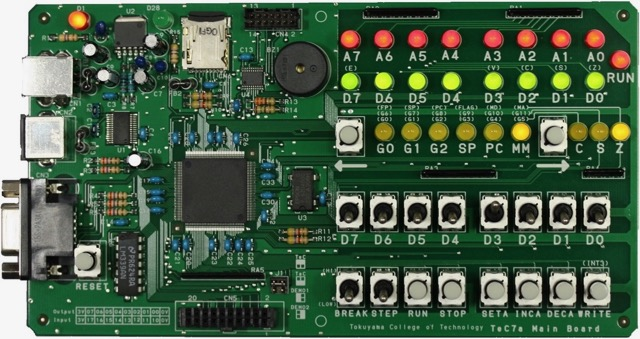
\includegraphics[scale=0.35]{Photo/TeC7.jpg}\\
(a) TeC7の写真
\end{center}
\end{minipage}
\begin{minipage}{0.38\columnwidth}
\begin{center}
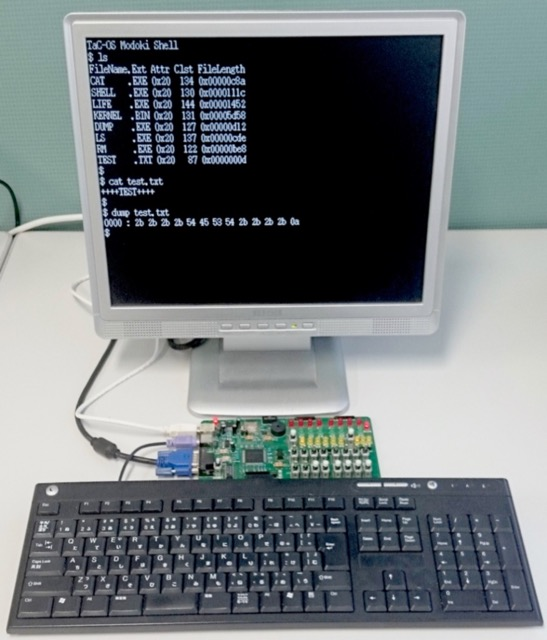
\includegraphics[scale=0.29]{Photo/TaC.jpg}\\
(b) TaCとしての使用例
\end{center}
\end{minipage}
\end{myfig}

TaC上では{\cmm}言語\footnote{
C言語に似た言語,
詳細は\url{https://github.com/tctsigemura/C--/blob/master/doc/cmm.pdf}を
参照のこと.}で記述されたTacOS\footnote{
詳細は\url{https://github.com/tctsigemura/TacOS}を参照のこと.} が動作する.
本書ではTacOSをオペレーティングシステムの実装例として参照する.

\subsection{ハードウェア構成}
\figref{tacBlock}にTaCのハードウェア構成を示す.
16ビットのシングルプロセッサ(CPUが一つ),
主記憶64KiBの非常に単純なシステムである.
単純なのでオペレーティングシステムの構築も容易である.
TaCに関する資料を付録\ref{appTac}にまとめる.

\myfigure{btp}{scale=0.48}{Fig/tacBlock-crop.pdf}
{TaCのハードウェア構成}{tacBlock}

\begin{itemize}
\item {\bf コンソールパネル} \\
\figref{tacPhoto}「(a) TeC7の写真」で,
TeC7本体右半分のランプやスイッチで構成される部分をコンソールパネルと呼ぶ.
コンソールパネルはCPUや主記憶と直接接続されており,
CPUを停止した状態で,
CPUや主記憶の内容を操作したり観察したりすることができる.
また,機械語命令を一命令毎に実行するステップ実行機能や,
ある番地の命令を実行した時点でプログラムを停止する
ブレーク機能ポイントが利用できる.
コンソールパネルの機能はハードウェアで実現されているので,
オペレーティングシステムの内部をステップ実行することも可能である.
TacOSの開発では,コンソールパネルがデバッグに活用された.

\item {\bf CPU} \\
\figref{tacRegPsw}に示すようなCPUレジスタとPSWを持つ16ビットCPUである.
PSWのフラグに実行モードを表すPビットを持ち,
カーネルモードとユーザモードを切り換えることができる.
機械語命令は,\figref{tacInsTbl}に示す46種類が準備されている.
機械語命令のアドレッシングモードは8種類ある.

\item {\bf メモリ} \\
メモリは\figref{tacMap}に示す構成である.
メモリ空間全体で64KiB,
自由に使用できるメモリが56KiB,
2KiBのVRAMと4KiBのIPL,32Bの割込みベクタからなる.
メモリは8ビット単位,または,16ビット単位で読み書きできる.
16ビット単位の場合は偶数アドレスを用いる.

\item {\bf タイマー} \\
$1$ミリ秒から$2^{16}-1$ミリ秒までの間隔で割込みを発生する
インターバルタイマーが二つ利用可能である.

\item {\bf ディスプレイアダプタ} \\
80文字×24行の文字をVGAディスプレイに表示する.
メモリ空間の{\tt E000h}から配置されるVRAMに書き込んだ
ASCIIコードと対応する文字をディスプレイに表示する.
{\tt E000h}番地がディスプレイの左上隅に対応する,
{\tt E001h}番地が一行目の2文字の位置,
{\tt E04Fh}番地が一行目の80文字の位置,
{\tt E050h}番地が二行目の1文字の位置に対応する.

\item {\bf SPIホストコントローラ} \\
スロットに挿入されたμSDカードをSPIモードに切換え読み書きを行う.
SPIホストコントローラに初期化コマンドを発行すると,
μSDカードをSPIモードに切換える.
ブロックアドレスとメモリアドレスを設定して読み出しコマンドを発行すると,
μSDカードの指定したブロックから512バイトのデータを
CPUを介さずに(DMA:Direct Memory Accessを用いて)メモリに読み出す.
書込みコマンドを発行すると,
メモリから指定ブロックにデータを書き込む.

\item {\bf シリアル通信インタフェース} \\
調歩同期方式,9,600Baudの通信インタフェースである.
USBシリアル変換ICを通してPC等のシリアルターミナルと通信できる.
1バイト転送する毎に割込みを発生する.

\end{itemize}

\subsection{TacOS}
\myfigure{btp}{scale=0.66}{Fig/tacosOrganization-crop.pdf}
{TacOSの構成}{tacosOrganization}

\figref{tacosOrganization}にTaC用のOSであるTacOSの構造を示す.
マイクロカーネルがプロセス間通信(IPC)機能を提供し,
サーバプロセスがメモリ管理やファイルシステム機能を提供する.
\figref{microkernel}の一般的なマイクロカーネル方式と異なり,
サーバプロセスがカーネルモードで動作しハードウェアに直接アクセスする.
また,サーバプロセスはマイクロカーネルと同じアドレス空間で動作するので,
カーネル内ルーチンをCALL機械語命令で直接に呼び出すことができる.

割込みやSVC命令の実行が原因で,
ユーザプロセスはカーネルモードに切り換わり
マイクロカーネル内の割込みハンドラが呼び出される.
割り込みハンドラで割込み原因を判断し,
マイクロカーネル内のルーチンを呼び出したり,
サーバプロセスの機能をIPCを用いて呼び出したりする.

\section{もう一つの仮想マシン}

\ref{osRole}で述べたように,
オペレーティングシステムは抽象化され便利な拡張マシン(仮想マシン)を,
必要な数だけ提供する.
ここで述べた仮想マシンは,単一ユーザ・プロセスの実行環境のことである.
同じ「仮想マシン」と言う用語が,
オペレーティングシステムを実行することが可能な,
よりハードウェアを忠実に再現した仮想マシンを指す場合もある.
ここでは,
一台のコンピュータ上で複数のオペレーティングシステムを実行可能な,
もう一つの仮想マシンについて紹介する.

\subsection{Type 2 ハイパーバイザ}
例えば,
Macを使用している人がWindowsでしか動作しないアプリケーションを使用する
場合を想像してしてみる\footnote{
徳山高専情報電子工学科のパソコン室では,
WindowsやLinuxでしか動作しないXilinx ISE WebPACKをMacで使用している.}.
予めMacのハードディスクにmacOSとは別にWindowsもインストールしておき,
電源投入時にmacOSとWindowsを選んでブートする方法もあるが,
オペレーティングシステムを切換える度にコンピュータを再起動するのは不便である.
また,macOSのアプリケーションとWindowsのアプリケーションを同時に実行したい
場合もある.

そこで,\figref{type2Hypervisor}に示すような
「Type 2 ハイパーバイザ(Type 2 Hypervisor)」を用いた仮想化が用いられる.
ハイパーバイザは
{\bf ホスト・オペレーティングシステム}の一つのユーザプロセスとして実行され,
コンピュータ一台の機能をエミュレーションする.
ハイパーバイザがエミュレーションするコンピュータの中で,
{\bf ゲスト・オペレーティングシステム}が稼働する.
エミュレーションはソフトウェアだけで完全に行うのではなく\footnote{
完全にソフトウェアで行う場合もある.},
ハードウェアの支援を受けて行うので高速に行うことができる\cite{virtualization}.
Type 2 ハイパーバイザとして有名は製品は,
VMware Workstation,
VMware Fusion,
VirtualBox\footnote{
徳山高専情報電子工学科のパソコン室では
macOS上のVirtualBoxでWindowsを動作させている.
%このWindowsの中でXlinix ISE WebPACKが使用できる.
}等である.

\myfigure{btp}{scale=0.66}{Fig/type2Hypervisor-crop.pdf}
{Type 2 ハイパーバイザ}{type2Hypervisor}

\subsection{Type 1 ハイパーバイザ}
メインフレーム上で1960年代から使用されている方式である.
現在ではPCサーバの仮想化にも使用されている.
Type 1 ハイパーバイザはホスト・オペレーティングシステム無しに
ハードウェア上で直接実行される.
Type 1 ハイパーバイザとして有名な製品は,
IBM z/VM,
VMware vSphere,
Xen,
Hyper-V等である.

サーバ向けの製品が主流であり,
例えば VMware vSphere は
実行中のゲストを他の物理サーバに移動する等,
非常に高度な機能を持っており\cite{vsphere},
一台のサーバ上に効率よく多数の仮想マシンを動かすことができる.
徳山高専情報電子工学科のパソコン室でも,
2台のサーバ上に50台の仮想デスクトップマシンを動かしていたことがある.

\myfigure{btp}{scale=0.66}{Fig/type1Hypervisor-crop.pdf}
{Type 1 ハイパーバイザ}{type1Hypervisor}

\subsection{仮想アプライアンス}
ゲスト・オペレーティングシステムとアプリケーションまでインストールし,
すぐに使用できる状態で配布される仮想マシンである.
例えば,メールフィルタソフトをインストールした仮想マシンを
入手しハイパーバイザで実行するだけですぐにメールフィルタリングが開始できる.

同じ手法で,
すぐに使用できるパーソナルコンピュータ用の
デスクトップ・オペレーティングシステムが配布されている場合もある.
Linux の一種であるUbuntuの場合,
VirtulBoxですぐに実行できるディスクイメージがダウンロードできる\cite{ubuntu}.
仮想アプライアンスは,
ソフトウェアの新しい流通手法である.

\section{まとめ}
本書は{\bf SMP(対称型マルチプロセッシング:Symmetric Multiprocessing)}の
コンピュータを前提にしている.
CPUは{\bf PSW(Program Status Word)}と{\bf CPUレジスタ}を含んでいる.
最近のIntel社のCPUでは,従来のCPUを{\bf Core(コア)},
複数のコアを含んだLSIのことをCPUと呼ぶ.

オペレーティングシステムのカーネルは,
割込みハンドラ,ディスパッチャ,サービスモジュール,
デバイスドライバ等から構成される.
ユーザ・プロセスからカーネルへの切換え原因は{\bf 割込み}だけである.
ユーザ・プロセス毎に{\bf 仮想CPU},{\bf 仮想メモリ空間},管理情報等を
持っている.

カーネルの構成方式には,
{\bf 単層カーネル(モノリシック・カーネル)}方式と
{\bf マイクロカーネル(micro-kernel)}方式の二種類があった.
マイクロカーネル方式ではサービスモジュールをサーバ・プロセスとし,
{\bf IPC(プロセス間通信)}を用いてサービスを要求する.
サービスモジュール間の独立性が高くなり高信頼性のシステムを構成可能であるが,
IPCはオーバーヘッドが大きい.
信頼性と性能はトレードオフの関係にある.

{\bf TaC}は,本書でオペレーティングシステムの実装例として使用する
TacOSを稼働させるコンピュータである.
コンソールパネルを持ち,
TacOSのカーネル内までステップ実行によるトレースが可能である.
{\bf TacOS}はマイクロカーネル方式の簡単なオペレーティングシステムである.
本書では,しばしばTacOSのソースコードを実装例として参照する.




 % 前提知識

\part{CPU管理}
\chapter{CPUの仮想化}
オペレーティングシステムは,
ハードウェアを抽象化した使いやすい拡張マシン(仮想マシン)を
必要な数だけ提供する.
数に限りがある資源は,必要な数だけあるように見せるために仮想化が行われる.
CPU資源も仮想化し,各プロセスが自分専用のCPUを持っているように見せかける.

%==============================================================================
\section{時分割多重}
CPUを仮想化するためには時分割多重が用いられる.
ハードウェアである実CPUの数は限られているので,
時間を区切って実CPUを使用するプロセスを次々に切換えていく.
\figref{virtualCPU}にCPU仮想化の原理を示す.

\begin{myfig}{btp}{時分割多重によるCPUの仮想化}{virtualCPU}
  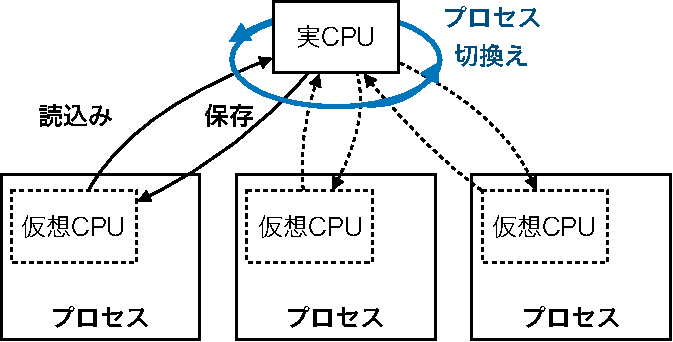
\includegraphics[scale=0.7]{Fig/virtualCPU-crop.pdf}
\end{myfig}

実CPUは\figref{cpuBlock}のような構造をもつハードウェアである.
プロセスの構造は\figref{procOrganization}に示した通りであり,
仮想CPUを含んでいる.
実CPUが短時間(例えば10ms)に次々と実行するプロセスを切換えていくことで,
複数のプロセスが夫々に専用のCPUを持ち並行して実行されているように見せかける.

CPUが実行するプロセスを切り換えるには,まず,
実CPUのコンテキストを現在のプロセスの仮想CPU領域に保存する.
次に,新しく実行するプロセスの仮想CPU領域から実CPUにコンテキストを読込み,
新しいプロセスの実行を再開する.
一つのプロセスから別のプロセスに切換える処理を
\emph{コンテキストスイッチ}と呼ぶ.
また,実CPUにコンテキストを読込んで実行を再開することを\emph{ディスパッチ},
ディスパッチを行うプログラムを\emph{ディスパッチャ}と呼ぶ.
\figref{osOrganization}にもディスパッチャは描かれていた.

%==============================================================================
\section{プロセスの状態}
\label{procState}
プロセスは,
キーボード等の入出力装置からの入力を待つ状態になったり,
時間が経過するのを待つ状態になったりする.
\emph{待ち(Waiting)状態}のプロセスにはCPUを割当てる必要がない.
このようにプロセスは幾つかの状態を持っている.
プロセスの状態はUNIXではpsコマンドで確認できる.
プロセスを模式的に示した\figref{procOrganization}では,
「プロセス情報」の「プロセスの状態」のことである.

\subsection{基本的な三つの状態}
\figref{procState}にプロセスの状態遷移図を示す.
この図は最も簡単なものであり,
実際のオペレーティングシステムでは,
もっと状態数が多くなる\footnote{
  macOSのpsコマンドのオンラインマニュアルで確認すると,
  macOSではプロセスの状態が,
  I(Idle),
  R(Runnable),
  S(Sleep),
  T(sTopped),
  U(Uninterruptible wait),
  Z(Zombie)の六つであることが分かる.}.
図に示された三つの状態を説明する.

\begin{itemize}
\item \emph{Ready(実行可能)} \\
  CPUを割当てれば実行を開始できる状態のことである.
  プロセスはCPUが割当てられるのを待っている.
\item \emph{Running(実行中)} \\
  CPUが割当てられ実行している状態のことである.
  CPUの数より多くのプロセスが同時にRunningになることはできない.
\item \emph{Waiting(待ち)} \\
  シグナルの到着や入出力の完了等の事象(イベント)を待っている状態である.
  プロセスは実行することができない.
\end{itemize}

\begin{myfig}{btp}{プロセスの状態遷移}{procState}
  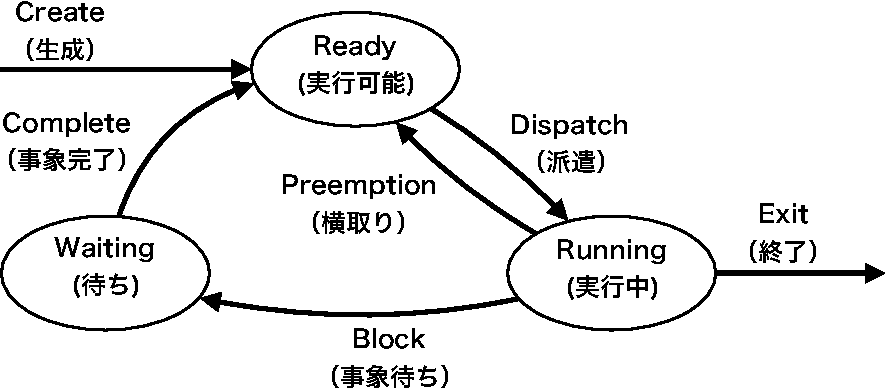
\includegraphics[scale=0.66]{Fig/procState-crop.pdf}
\end{myfig}

\subsection{状態遷移}
\figref{procState}に示された六つの状態遷移の意味は以下の通りである.

\begin{enumerate}
\item \emph{Create(クリエート,生成)} \\
  新しいプロセスが生成されるとReady状態になる.
  親プロセスが\|fork()|システムコール(UNIXの場合)や
  \|CreateProcess()|システムコール(Windowsの場合)を実行すると,
  新しい子プロセスが生成される.
\item \emph{Dispatch(ディスパッチ,派遣)} \\
  Ready状態のプロセスは,
  自分の順番が来たらCPUが割当てられRunning状態に遷移し実行を開始する.
\item \emph{Preemption(プリエンプション,横取り)} \\
  Running状態のプロセスは,
  決められた時間(クオンタムタイム)を使い切ったときや,
  より優先度の高いプロセスがReady状態になったとき,
  CPUを取り上げられReady状態に遷移する.
\item \emph{Block(ブロック,事象待ち)} \\
  Running状態のプロセスが,
  システムコールを発行して自らWaiting状態に遷移することがある.
  例えば入出力システムコール
  (\|open()|,\|read()|,\|write()|,\|close()|等)や,
  シグナル待ちシステムコール(\|pause()|,\|wait()|,\|sleep()|等)
  を発行した場合である.
  また,他のプロセスからシグナルを受信した場合も,
  Waiting状態に遷移することがある.
  更に,仮想記憶の機能を持つオペレーティングシステムでは,
  プロセスが読み書きしようとした領域がメモリ上に存在しない時も
  この遷移が起こり,
  メモリ領域を確保するための処理がカーネル内部で始まる.
\item \emph{Complete(コンプリート,事象完了)} \\
  Waiting状態のプロセスは,
  入出力の完了やシグナルの発生等の事象(イベント)が発生すると
  Ready状態に遷移する.
  Waiting状態のプロセスは停止しているのでプロセスが事象を発生することはない.
  事象はプロセスの外部からもたらされる.
\item \emph{Exit(終了)} \\
  プロセスが自ら\|exit()|システムコール(UNIXの場合)や
  \|ExitProcess()|システムコール(Windowsの場合)を用いて終了する場合,
  または,プロセスがシグナルを受ける等して終了させられる場合に,
  この遷移が起こる.
  シグナルはプロセス(他プロセス,自プロセス)から明示的に送信される場合と,
  自プロセスが保護違反などのエラーを起こして発信される場合がある.
\end{enumerate}

%==============================================================================
\section{プロセスの切換え(コンテキストスイッチ)}
Running状態のプロセスがBlock遷移またはPreemption遷移しCPUを取り上げられると,
他のReady状態のプロセスがCPUを割付けられDispatch遷移し実行を再開する.

\subsection{切換えの原因}
Running状態のプロセスが状態遷移を起こす原因を以下にまとめ直す.

\begin{enumerate}
\item イベント \\
  Running状態のプロセスは,
  自ら「システムコールを発行」することでBlock遷移をすることがある.
  また,他のプロセスからの「\emph{干渉}\footnote{
      干渉には,より優先順位の高いプロセスが実行可能になった,
      別のプロセスからシグナル等を受取った等がある.}
    を受け」Block遷移することがある.
\item タイムスライシング \\
  Running状態のプロセスが長時間の実行を続けるとPreemption遷移をする.
  一度に実行しても良い時間(クオンタムタイム)を使い切ったためである.
  Ready状態のプロセスが他にあれば,そのプロセスに実行が切換わる.
  他に実行すべきプロセスが無い場合は,再度,同じプロセスが実行される.
\end{enumerate}

\subsection{切換え手順}
\figref{procSwitch}に二つのプロセス間で実行が切り換わる様子を示す.
図では時間に従って上から下へ処理が進む.
左側はプロセスAの実行を,
右側はプロセスBに実行を,
中央はカーネルの実行を表している.
以下では,
図の上半分でプロセスAからプロセスBに実行が切り替わる手順を説明する.
図の下半分の説明は省略するが,
上半分と同様な手順でプロセスBからプロセスAに切り替わる手順を示している.

\begin{myfig}{btp}{プロセスの切換え}{procSwitch}
  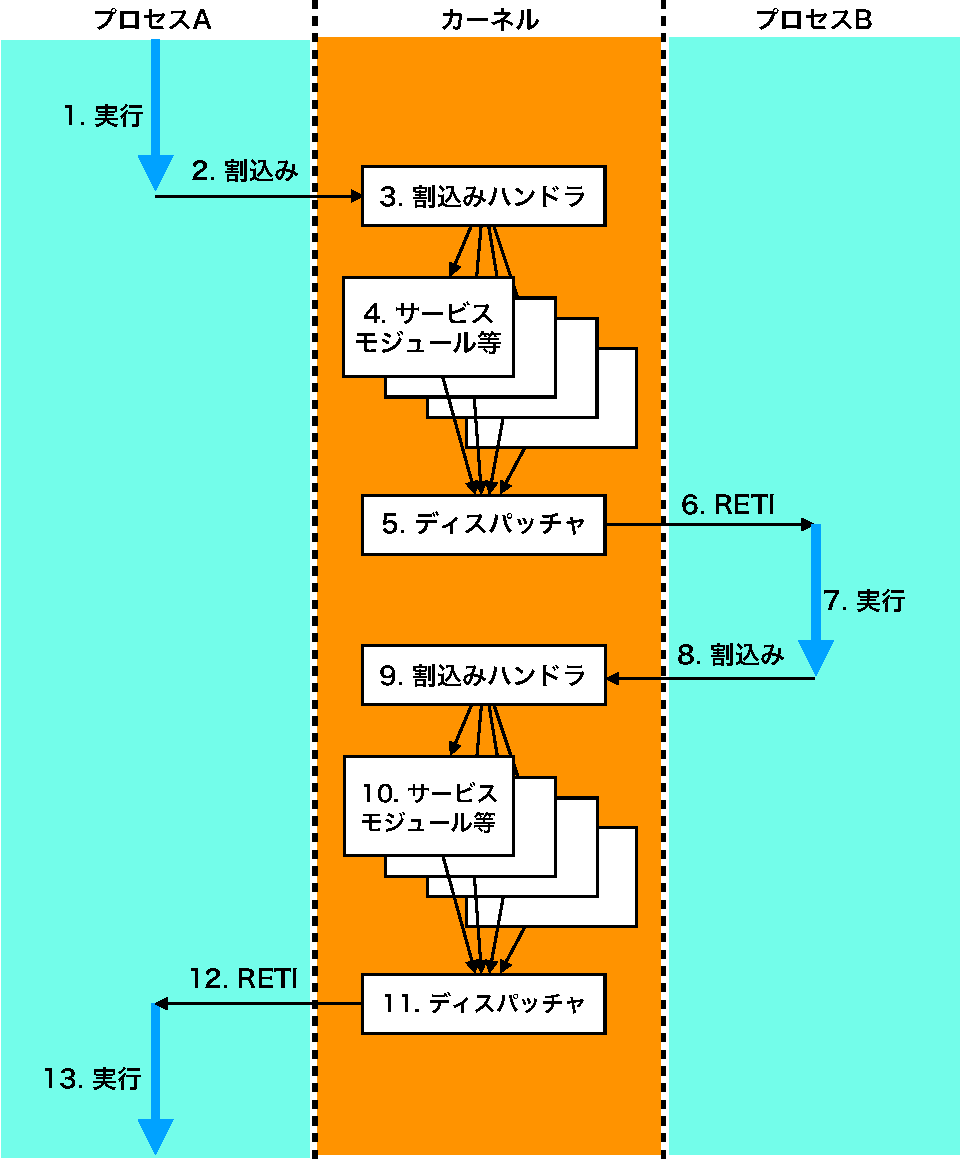
\includegraphics[scale=0.6]{Fig/procSwitch-crop.pdf}
\end{myfig}

\begin{enumerate}
\item 実行 \\
  日頃はCPUがユーザ・プロセスを実行している.
\item 割込み \\
  割込みが発生し処理がプロセスAからカーネル内の割込みハンドラに移る.
  割込みの原因は\ref{interruptSource}で述べた様々なものが考えられる.
  割込みが発生すると以下の処理が\emph{CPUのハードウェアにより自動的に}される.
  \begin{enumerate}
  \item CPUの(PCを含む)PSWがスタックに保存される.
  \item CPUの実行モードがカーネルモードに切り換わる.
  \item 割込みハンドラにジャンプする.
  \end{enumerate}
\item 割込みハンドラ \\
  PSW(スタック上にある)とCPUレジスタ(\figref{cpuBlock}参照)からなる
  プロセスのコンテキストを
  プロセスの仮想CPU領域(\figref{procOrganization}参照)に保存する.
  次に割込み原因を調べ,
  割込み原因に応じた処理(サービスモジュール等)にジャンプする.
  例えば,
  割込み原因が\|open()|システムコールなら,
  openシステムコールの処理を行うファイルシステムの
  サービスモジュールにジャンプする.
  割込み原因がI/O完了なら,
  完了したI/Oに対応するデバイスドライバにジャンプする.
\item サービスモジュール等 \\
  サービスモジュールやデバイスドライバが割込み原因に応じた処理を行う.
  この過程でプロセスの状態が変化することがある.
  例えば,プロセスが発行したシステムコールが原因でBlock遷移する場合や,
  タイマーやI/Oの完了割込によりWaiting状態だった別のプロセスが
  Complete遷移する場合,
  タイマーの完了割込により現在のプロセスがPreemption遷移する場合等が
  考えられる.
  サービスモジュール等の処理が完了するとディスパッチャにジャンプする.
\item ディスパッチャ \\
  実行可能なプロセスの中から一つを選び,
  選んだプロセスの仮想CPU領域の内容をCPUレジスタにロードする.
  最後にPSWを復旧する機械語命令(RETI)を実行しプロセスの実行に戻る.
\item RETI \\
  PSWを復旧する機械語命令として
  割込復帰用の\emph{RETI(RETurn from Interrupt)命令}を用いる.
  RETI命令は単一の命令でPSW(PCとフラグ)を一度にスタックから復旧する.
  CPUの実行モードを表すフラグはPSWに含まれているので,
  PSWが復旧されることで実行モードがカーネルモードからユーザモードに切り換わる.
\item 実行 \\
  新しく選択されたユーザ・プロセスが実行される.
\end{enumerate}

\subsection{切換えの例}
計算に長い時間を要する二つのプロセスだけがある時,
クオンタムタイムを使い切ってもう一方のプロセスに切り換わり,
交互に実行される様子を\figref{procSwitchInst}に示す.
以下に手順を説明する.

\begin{myfig}{btp}{プロセスの切換えの例}{procSwitchInst}
  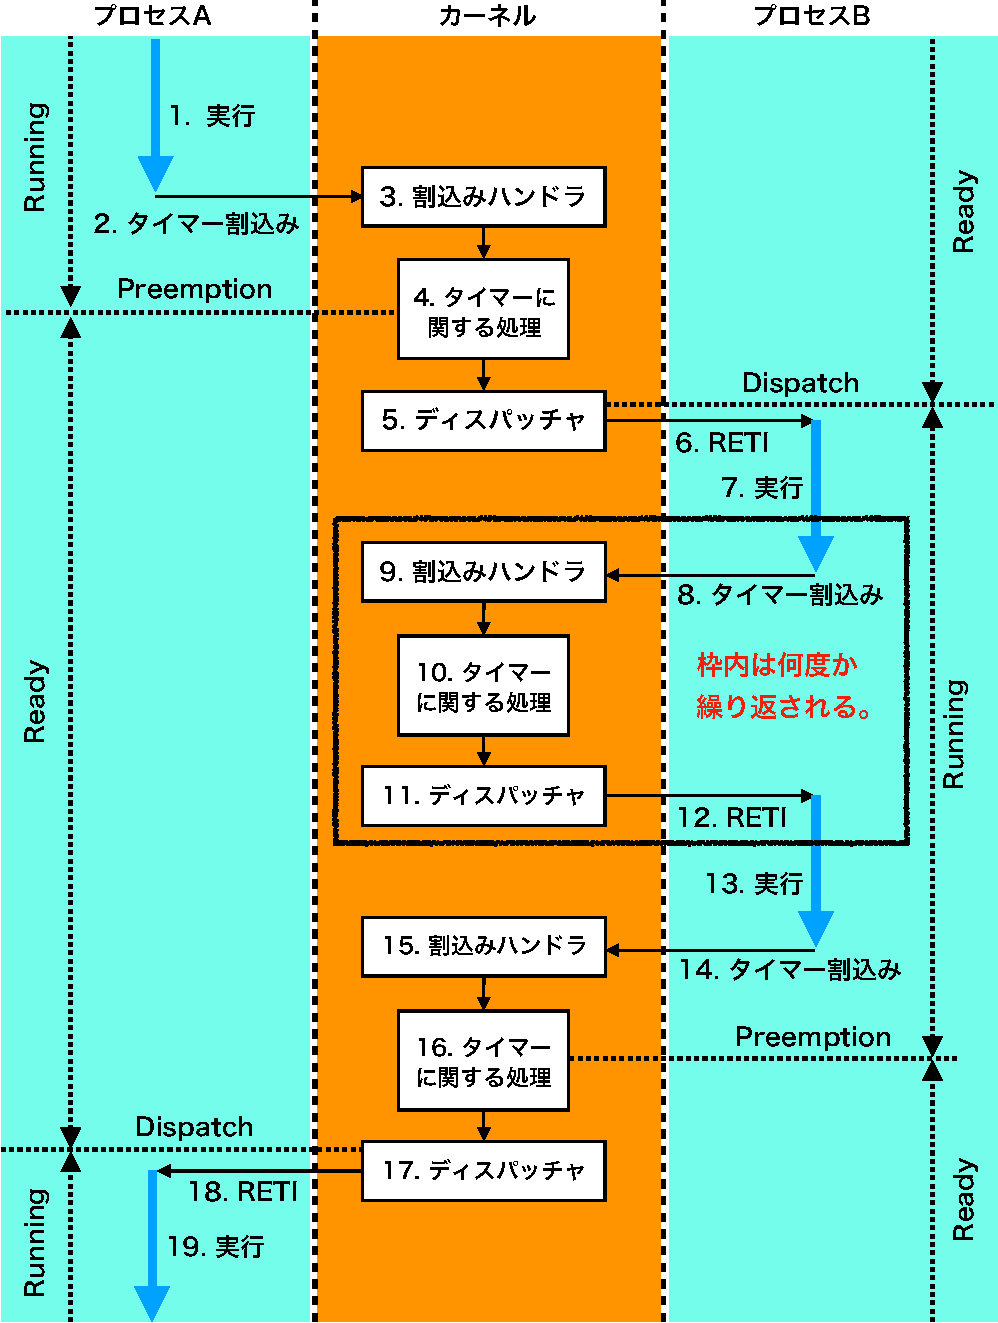
\includegraphics[scale=0.6]{Fig/procSwitchInst-crop.pdf}
\end{myfig}

\begin{enumerate}
\item 実行 \\
  プロセスAは計算処理を続けている.
  長い時間に渡ってシステムコールを発行することは無い.
\item タイマー割込み \\
  タイマーは一定間隔で割込みを発生する.
  割込が発生するとCPUのハードウェアが自動的にPSWを保存し,
  割込みハンドラにジャンプする.
  オペレーティングシステムは,
  主に,この割込みを基準に時間の経過を認識する.
\item 割込みハンドラ \\
  プロセスのコンテキストをプロセスの仮想CPUに保存する.
  その後,割込原因を調べタイマーからの割込みなので,
  「タイマーに関する処理」を行うカーネル内のモジュールへジャンプする.
\item タイマーに関する処理 \\
  一定間隔で発生するタイマーからの割込みを利用して,
  システムの時計を進めたり,
  リソース(CPUやメモリ等)の利用統計データを更新したりする.
  その間にプロセスAがクオンタムタイムを使い切ったことが判明すると,
  プロセスAをPreemption遷移させる.
  この時点でプロセスAの状態がReadyに変化する.
\item ディスパッチャ \\
  Ready状態のプロセスの中から適切な一つを選びDispatch遷移させる.
  \figref{procSwitchInst}はプロセスBが選択された場合である.
  ディスパッチャはプロセスBのCPUレジスタを復旧する.
\item RETI \\
  プロセスBのPSWを復旧し,プロセスBの実行を再開する.
\item 実行 \\
  プロセスBは計算処理を再開する.
  プロセスBも長い時間計算を続けるプロセスとする.
\item タイマー割込み \\
  計算を続けるうちにタイマーからの割込みが発生する.
\item 割込みハンドラ \\
  プロセスBのコンテキストを保存する.
\item タイマーに関する処理 \\
  プロセスBは,まだ,クオンタムタイムを使い切っていないので,
  Preemptionは発生しない.
\item ディスパッチャ \\
  Preemptionは発生しないので,
  プロセスBのコンテキストを復旧する.
\item RETI \\
  プロセスBに戻る.
\item 実行 \\
  プロセスBは計算処理を再開する.
\item タイマー割込み \\
  8.〜13. を何度か繰り返し,
  クオンタムタイムを使い切った時のタイマー割込みである.
\item 割込みハンドラ \\
  プロセスBのコンテキストを保存する.
\item タイマーに関する処理 \\
  クオンタムタイムを使い切ったのでPreemptionが発生する.
\item ディスパッチャ \\
  Ready状態のプロセスAを選択しDispatch遷移させる.
  プロセスAのコンテキストを復旧する.
\item RETI \\
  プロセスAに戻る.
\item 実行 \\
  プロセスAは計算処理を再開する.
\end{enumerate}

%==============================================================================
\section{PCB(Process Control Block)}
PCBはプロセスを表現する重要なカーネル内のデータ構造である.
PCBはカーネル内のプロセステーブルに格納される.

\subsection{PCBの内容}
PCBは,\figref{procOrganization}の
「仮想CPU」と「プロセス情報」を合わせたものに相当する.
PCBには以下のような情報が格納される.

\begin{itemize}
\item 仮想CPU
\item プロセス番号
\item 状態(Running,Waiting,Ready等)
\item 優先度
\item 統計情報(CPU利用時間等)
\item 次回のアラーム時刻
\item 親プロセス
\item 子プロセス一覧
\item シグナルハンドリング
\item 使用中のメモリ
\item オープン中のファイル
\item カレントディレクトリ
\item プロセス所有者のユーザ番号
\item PCBのリストを作るためのポインタ
\end{itemize}

\subsection{PCBリスト}
カーネル内ではPCBがプロセスを表現する.
例えば,優先順にソートされたReady状態のプロセスのリストは,
優先度をキーにソートされたPCBの線形リスト(\emph{待ち行列})として表現される.
この線形リストを\emph{実行可能列}と呼ぶ.
その様子を\figref{procQueue}に示す.
図は,数値が小さいほど優先度が高い意味になっている.

\begin{myfig}{btp}{PCBのリスト}{procQueue}
  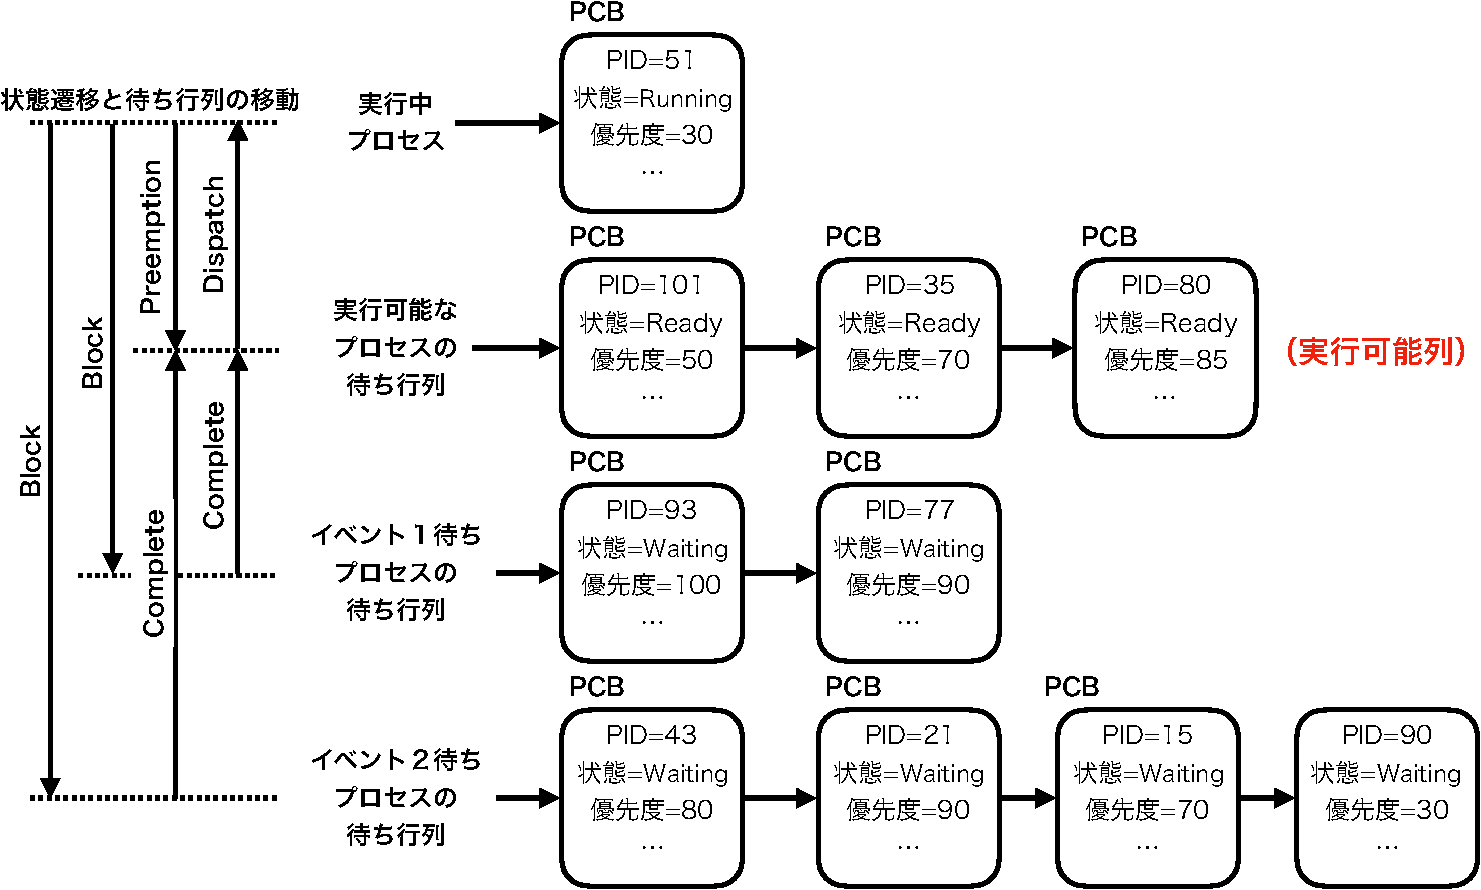
\includegraphics[scale=0.55]{Fig/procQueue-crop.pdf}
\end{myfig}

Ready状態のプロセスだけでなく,
Running状態のプロセスや,
Waiting状態のプロセスも待ち行列で管理される.
Waiting状態のプロセスは,
待ち合わせているイベント毎に待ち行列を作っている.
イベント待ち行列のソート順はイベント毎にルールが決められる.

プロセスの状態遷移に合わせてPCBが待ち行列の間を移動する.
\figref{procQueue}の左側の「状態遷移と待ち行列の移動」が
「どの待ち行列から,どの待ち行列に移動可能か」を表している.
例えば,Running状態(実行中)のプロセスがPreemption遷移をすると,
状態がReadyに変わるだけでなく,
PCBが「実行可能なプロセスの待ち行列」に移動する.
この移動ルールは\figref{procState}の状態遷移と一致している.

%==============================================================================
\section{スレッド(Thread)}
ここまで,一つのプロセスが一つの仮想CPUを持つモデルを考えてきた.
しかし,実際のコンピュータハードウェアはCPUを複数持つSMPの場合もある.
これでは
「ハードウェアの機能を抽象化した便利な\emph{拡張マシン}」
(\ref{abstruction}参照)であるはずのプロセスが,
「CPUが一つしかない\emph{縮小マシン}」なっている.
そこで,SMPに対応しプロセスが複数の仮想CPUを持つモデルを導入する.
これにより,一つのプロセスが
並列実行する複数の処理の流れ(スレッド)を持つことが可能になる.

\subsection{スレッドの役割}
複数のプロセス(ジョブ)を主記憶にロードしておくことで
CPUの利用効率を高くできることは既に説明した
(\pageref{multiprogramming}ページ,マルチプログラミング参照).
マルチプログラミングの,もう一つのメリットは,
プログラミングが簡単になる場合があることである.
以下ではWebサーバを例に,
マルチプログラミングによる改善を紹介する.

\begin{itemize}
\item マルチプロラミングなし \\
  \figref{singleProcSingleClient}に最も簡単なモデルを示す.
  Webサーバはリクエストを受信すると,それに対するレスポンスを返す.
  処理は1番目のクライアントから順に行われ,
  2番目のクライアントは1番目の処理が終了するまで待たされる.
  このモデルの問題点は,
  処理中にWebサーバプロセスがI/O待ち等でブロック(Block)する可能性があり,
  その間,他のクライアントへのサービスがされないことである.

  2番目以降のクライアントが長時間待たされないように,
  複数のクライアントの処理を並行してできるように改良したモデルが
  \figref{singleProcMultiClient}である.
  「I/O完了の監視」は通信を含む複数の入出力を同時に監視し,
  どれかが読み書き可能になるのを待つ機能である.
  UNIXでは\|select()|システムコールがこの機能を持つ.
  読み書き可能になったことを確認後に読み書きを行うので
  プロセスがブロックすることが無くなり,
  複数のクライアントに対して同時にサービスを行うことができる.

  しかし,Webサーバのプログラミングは難しくなる.
  一方のクライアントの処理が終わらないうちに,
  別のクライアントの処理を開始する必要があるからである.
  クライアント毎に処理がどこまで進んでいるのかを表す
  \emph{状態}を持つ必要がある.
  また,CPUが複数存在する場合でも,
  同時には一つのCPUしか働かないことも問題である.

  \begin{myfig}{btp}{マルチプログラミングを用いないWebサーバ}
    {singleProcSingleThread}
    \begin{minipage}{0.49\columnwidth}
      \begin{center}
        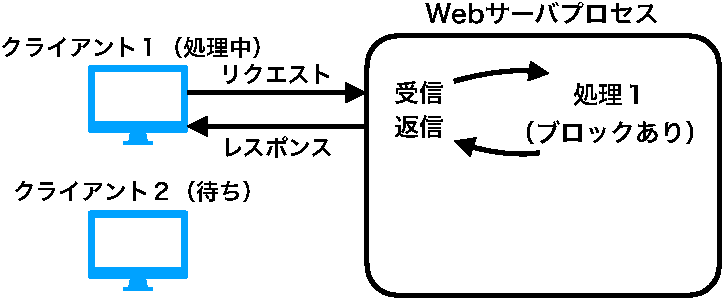
\includegraphics[scale=0.6]{Fig/singleProcSingleClient-crop.pdf}
        \subcaption{最も基本的なWebサーバのモデル}
        \label{fig:singleProcSingleClient}
      \end{center}
    \end{minipage}
    \begin{minipage}{0.49\columnwidth}
      \begin{center}
        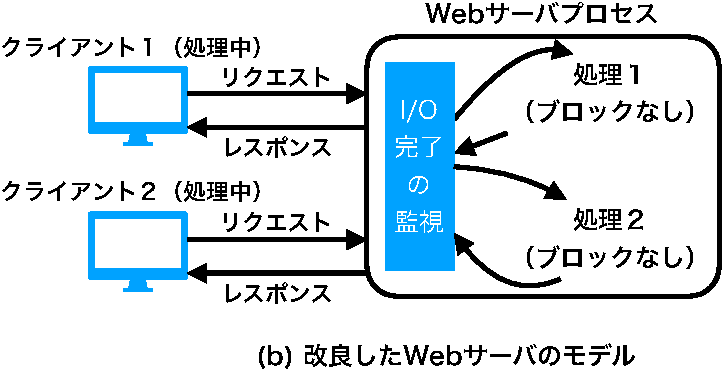
\includegraphics[scale=0.6]{Fig/singleProcMultiClient-crop.pdf}
        \subcaption{改良したWebサーバのモデル}
        \label{fig:singleProcMultiClient}
      \end{center}
    \end{minipage}
  \end{myfig}
  
\item マルチプロセス \\
  マルチプログラミングを用いることで前記の問題を解決したモデルを
  \figref{multiProc}に示す.
  Webサーバプロセスは,
  まず,接続要求を待ちクライアント1からの接続を受け入れる.
  次に,クライアント1専用のサーバプロセスを生成し処理を任せる.
  Webサーバプロセスは,
  生成したプロセスの終了を待たずに,
  次の接続要求待ちになる.
  クライアント2からの接続要求があったら
  クライアント2専用のサーバプロセスを生成し,
  接続要求待ちに戻る.

  このモデルなら,
  各クライアントの処理を別々のプロセスが行っているので,
  プロセスがブロックしても構わない.
  そのため,プログラミングは簡単になる.
  また,CPUが複数あればプロセスが真に並列に実行される.
  しかし,プロセスの生成はメモリ空間の確保や初期化を含み\emph{重い処理}である.
  また,
  プロセスはメモリを共有していないのでプロセス間の情報共有には効率が悪い.

\item マルチスレッド \\
  複数のスレッドを使用したモデルを\figref{multiThread}に示す.
  マルチプロセスの場合と良く似たプログラムであるが,
  クライアント毎に専用のプロセスを作る代わりに,
  クライアント毎に専用のスレッドを作る.
  スレッドの生成はプロセス生成より10〜100倍速いと
  言われている\cite{lightWeight}.
  また,スレッドはメモリを共有しているので情報共有には都合が良い.
  例えば,Webサーバが頻繁に参照されるページをメモリ上にキャッシュする場合,
  キャッシュをスレッドで共有できる.

  \begin{myfig}{btp}{マルチプログラミングを用いるWebサーバ}{multiPrograming}
    \begin{minipage}{0.49\columnwidth}
      \begin{center}
        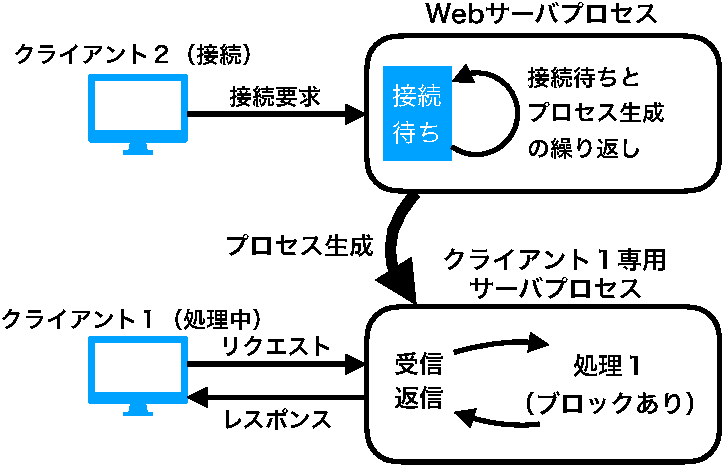
\includegraphics[scale=0.6]{Fig/multiProc-crop.pdf}
        \subcaption{マルチプロセスにしたWebサーバのモデル}
        \label{fig:multiProc}
      \end{center}
    \end{minipage}
    \begin{minipage}{0.49\columnwidth}
      \begin{center}
        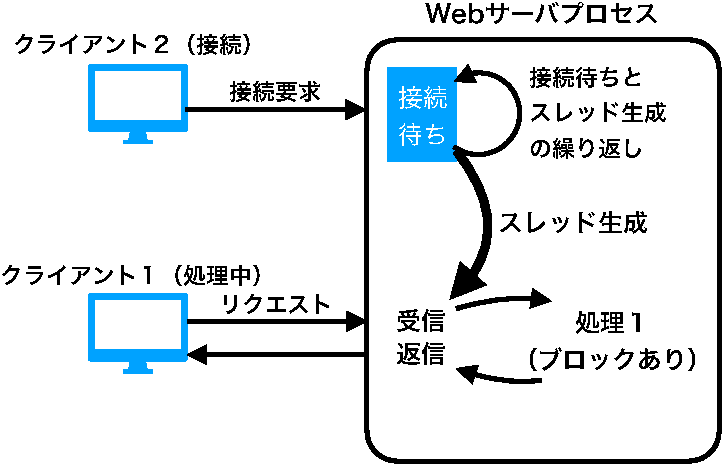
\includegraphics[scale=0.6]{Fig/multiThread-crop.pdf}
        \subcaption{改良したWebサーバのモデル}
        \label{fig:multiThread}
      \end{center}
    \end{minipage}
  \end{myfig}
\end{itemize}

\subsection{スレッドの形式}
読者は,「スレッドはカーネルが実現する」と暗黙のうちに考えていたかも知れない.
しかし,ユーザプログラム(ライブラリ)内でスレッドを実現することもある.
カーネルが実現するスレッドを\emph{カーネルスレッド},
ユーザプログラム内で実現するスレッドを\emph{ユーザスレッド}と呼ぶ.

\begin{myfig}{btp}{ユーザスレッドとカーネルスレッド}{threadOrganization}
  \begin{minipage}{0.49\columnwidth}
    \begin{center}
      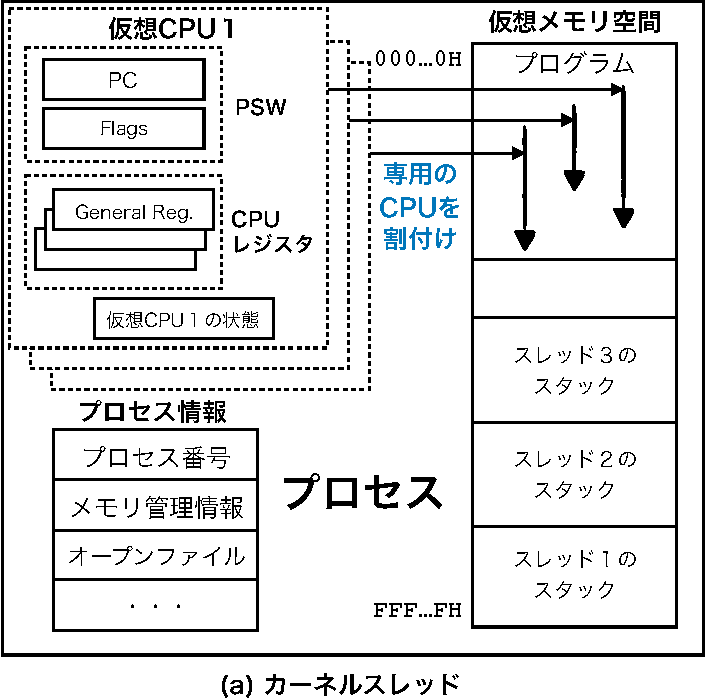
\includegraphics[scale=0.6]{Fig/kernelThread-crop.pdf}
      \subcaption{カーネルスレッド}
      \label{fig:kernelThread}
    \end{center}
  \end{minipage}
  \begin{minipage}{0.49\columnwidth}
    \begin{center}
      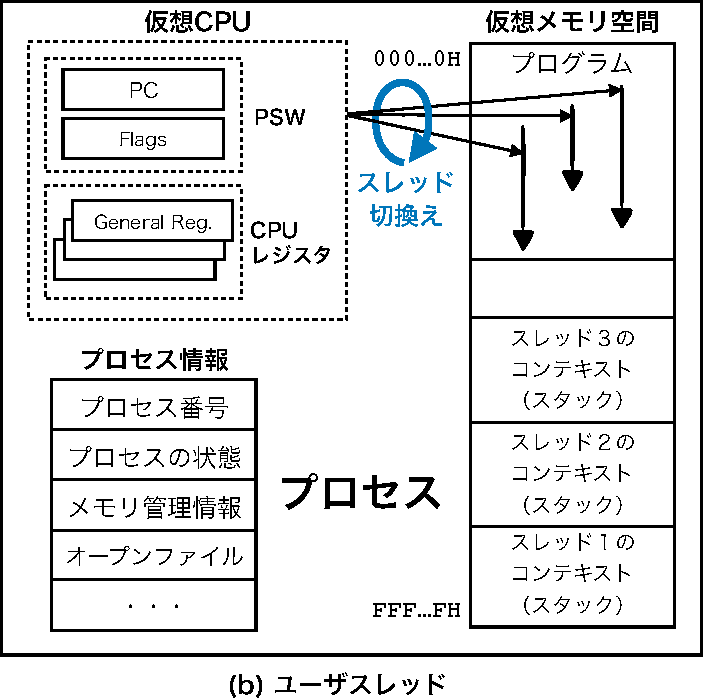
\includegraphics[scale=0.6]{Fig/userThread-crop.pdf}
      \subcaption{ユーザスレッド}
      \label{fig:userThread}
    \end{center}
  \end{minipage}
\end{myfig}

\begin{itemize}
\item \emph{カーネルスレッド} \\
  カーネルスレッドの模式図を\figref{kernelThread}に示す.
  カーネルスレッドはプロセスの仮想CPUを複数にし,
  仮想CPUがプログラムを並行して実行する.
  「プロセス情報」から「プロセスの状態」は無くなり,
  代わりに仮想CPU毎に「仮想CPUの状態」を管理するようになる.
  CPUが複数ある時,カーネルスレッドであれば,
  プロセス内を真に並列実行することが可能である.
\item \emph{ユーザスレッド} \\
  ユーザスレッドの模式図を\figref{userThread}に示す.
  プロセスには単一の仮想CPUしかない.
  ユーザスレッドは仮想CPUを時分割多重して実現される.
  カーネルを経由しないでスレッドの生成や切換えをすることができるので,
  オーバーヘッドが非常に小さい.
\end{itemize}

以下に述べるように,両者を組合せた三つのスレッドモデルが使用される.

\begin{enumerate}
\item \emph{One-to-One Model} \\
  全てのスレッドがカーネルスレッドのモデルである.
  \figref{kernelThread}に相当する.
  プロセス内にカーネルが管理する仮想CPUが複数あるので,
  複数プロセスと同等な並列実行が可能である.
  しかし,スレッドの生成や切換えにカーネルが介入するので,
  処理は重くなる.
  また,システムによっては生成できるスレッド数に制限がある.
\item \emph{Many-to-One Model} \\
  複数(Many)のユーザスレッドを
  一つ(One)のカーネルスレッドで実行するモデルである.
  \figref{userThread}に相当する.
  プロセス内にカーネルスレッドは一つしか存在しない.
  ユーザスレッドはユーザプログラム(ライブラリ)の工夫で
  単一のカーネルスレッドを複数に見せかけているだけなので,
  真の並列実行にはならない.
  また,何れかのスレッドがシステムコールでブロックすると,
  全てのスレッドが停止してしまう問題がある.
\item \emph{Many-to-Many Model} \\
  複数の(Many)のユーザスレッドを
  複数の(Many)のカーネルスレッドで実行するモデルである.
  カーネルスレッドの数をユーザスレッドの数より多くすることはない.
  前記二つのモデルの折衷案である.
\end{enumerate}

\subsection{スレッドプログラミング}
配列データの合計を求める処理をスレッドを用いて高速化する例を考えよう.
\figref{threadedSum}に原理を示す.
配列\|a|をM分割し個別スレッドで(CPUが複数あれば)同時に小計を計算する.
小計は配列\|total|に格納する.
最後に\|main|スレッドが\|total|の合計を求めると全体の合計\|sum|が計算できる.

\begin{myfig}{btp}{M個のスレッドで手分けして合計を計算する様子}{threadedSum}
  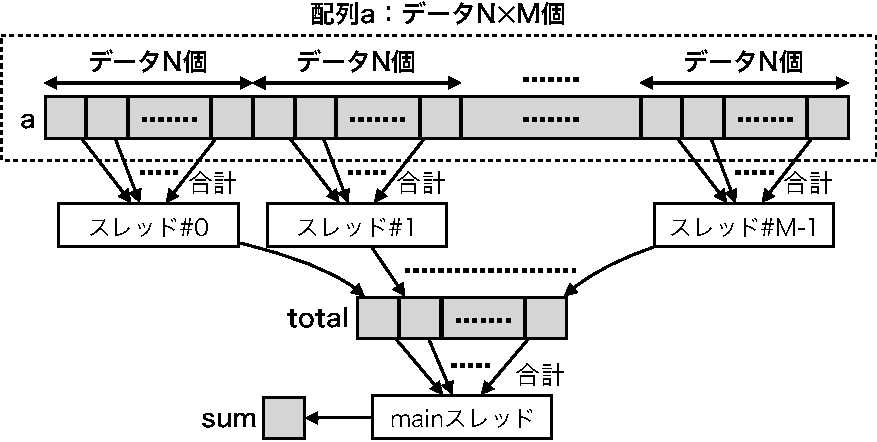
\includegraphics[scale=0.66]{Fig/threadedSum-crop.pdf}
\end{myfig}

\subsubsection{POSIXスレッドによる実装}
このアイデアをPOSIXスレッド\footnote{
  POSIXスレッドはUNIX系のオペレーティングシステムで使用できる.
}を用いたC言語プログラムにしたものをリスト\ref{threadTest}\footnote{
  このプログラムは macOS High Sierra で動作確認をした.
}に示す.

\lstinputlisting[numbers=left,float=btp,label=threadTest,
  caption=M個のスレッドで分担して配列データの合計を求めるプログラム]
  {SampleCode/pThread/threadTest.c}

12行の\|thread()|関数はM個のスレッドで同時に並列実行される.
配列\|a|の担当範囲等は引数\|arg|により指示される.
関数の引数(\|arg|)やローカル変数(\|args|,\|sum|,\|i|)は,
スレッドのスタック(\figref{threadOrganization}参照)に割付けられるので,
スレッド毎に別の実体を持つ.
グローバル変数\|a|や\|total|等は全てのスレッドで共有される.

32行の\|pthread_attr_init()|は引数の\|pthread_attr_t|型変数を
デフォルトのアトリビュート値で初期化する.
33行の\|pthread_create()|がスレッドを生成する関数である.
新しいスレッドの実行は引数で指定された\|thread()|関数から始まる.
\|pthread_create()|の引数\|p|は,
\|thread()|関数が実行を開始する時に\|arg|引数に渡される.

38行の\|pthread_join()|はスレッドの終了を待つ関数である.
スレッドの終了が確認できたら,39行で小計を\|sum|に足し込む.

\subsubsection{実行時間の計測結果}
リスト\ref{threadTest}のプログラムの実行時間を\tabref{threadTimeTbl}に,
グラフにしたものを\figref{threadTimeGrph}に示す
\footnote{
  実行時間の計測にはOS X の \texttt{time} コマンドを用いた.
}
\footnote{
  実行時間が短すぎて比較し難いので,
  プログラムの14行から17行を10万回繰り返すように改造した上で計測した.}
\footnote{
  計測に使用したコンピュータは
  OS X Yosemite をインストールした
  Mac Pro(Late 2013, 3.5GHz 6-Core Intel Xeon E5)である.
  %macOS High Sierra をインストールした
  %MacBook Pro(Retaina, 13-inch, Mid 2014, 2.8GHz Intel Core i5)である.
  C言語コンパイラは
  Apple LLVM version 7.0.0(clang-700.0.72)を使用した.
}.

\begin{mytable}{btp}{スレッド数による実行時間比較}{threadTimeTbl}
  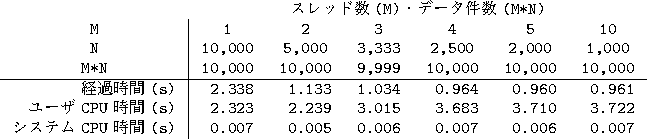
\includegraphics[scale=1.0]{Tbl/threadTimeTbl.pdf}
\end{mytable}

\begin{myfig}{btp}{スレッド数による実行時間の変化}{threadTimeGrph}
  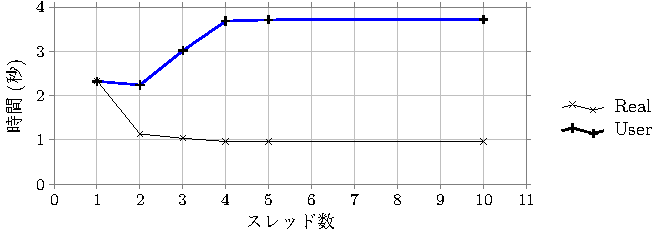
\includegraphics[scale=1.0]{Tbl/threadTimeGrph.pdf}
\end{myfig}

スレッド数が1の時は,経過時間(Real)とユーザCPU時間(User)が,
ほぼ,同じになる.
一つのコア\footnote{従来のCPUのこと.}が全力で合計を計算した結果である.

スレッド数が1〜6の間は,経過時間がスレッド数に反比例して短くなる.
合計の計算時間に対応するユーザCPU時間は,ほぼ一定である.
使用したコンピュータが持つ六つのコアが,
最大で六つのスレッドに割当てられ,
真に並列実行された結果である.

スレッドの数が6〜10に増加する間,経過時間は,ほぼ一定である.
しかしユーザCPU時間が増加している.
必要な計算量は一定なのに長いCPU時間を必要とするので,
コアの性能が悪化したように見える.

コアの性能が悪くなったように見えるのは,
ハイパースレッディング・テクノロジー\cite{hyperThreading}により,
コアの数が倍(12個)あるように見せかけているためである.
ハイパースレッディング・テクノロジーは,
単一スレッドを実行する場合は遊んでしまうコア内のユニットを,
二つのスレッドを同時に実行することで効率よく使用する技術である.
見かけ上コアの数が二倍になるが,合計の性能は二倍には達しないので,
コアあたりの性能が下がったように見える.
%\footnote{
%この計測結果からは,
%ハイパースレッディング・テクノロジーは,
%性能の改善に余り寄与していないように見える.
%}

%スレッド数を12以上にすると,
%(見かけ上の)コア全てが常時使用されるので,
%経過時間,ユーザ時間の合計のどちらも一定になる.

%==============================================================================
\section{CPU仮想化の実装例}
第\ref{tacosVirtualCPU}章にTacOSのCPU仮想化の例を示す.
この例は,{\cmml}で記述したカーネル内データ構造や,
プロセス切換えプログラム,プロセススケジューラ等の実装を含む.
また,プロセスのメモリ配置についても説明している.

%==============================================================================
\section{まとめ}
本章では,時分割多重によるCPUの仮想化について学んだ.
プロセスは幾つかの状態を持ち,
実行できない状態の場合はCPUを割当てない.
プロセスはイベントやタイムスライシングにより状態が変化する.
CPUは,実行を中断するプロセスから次に実行するプロセスに,
コンテキストスイッチを行う.

PCBはプロセスを表現するカーネル内の重要なデータ構造である.
例えばプロセスの待ち行列はPCBの待ち行列として表現されるし,
プロセスの実行が中断する時はPCBにコンテキストが保存される.

スレッドを導入することで,
SMPに対応したプロセスのモデルを表現できる.
スレッドにはカーネルスレッドとユーザスレッドがあった.
また,これらを組み合わせた三つのスレッドモデルがあった.
POSIXスレッドを用いてデータの合計を計算する処理を高速化する
プログラム例を紹介し,実行時間の計測結果を示した.
スレッド数がCPU(コア)数以内の場合は,
スレッド数に反比例して実行時間が短くなることが確認できた.

%==============================================================================
\section*{練習問題}
\begin{enumerate}
  \renewcommand{\labelenumi}{\ttfamily\arabic{chapter}.\arabic{enumi}}
  \setlength{\leftskip}{1em}
\item 次の言葉の意味を説明しなさい.
  \begin{enumerate}
    \item 時分割多重
    \item コンテキストスイッチ
    \item Dispatch(ディスパッチ)
    \item Preemption(プリエンプション)
    \item プロセスの状態
    \item プロセスの状態遷移
    \item RETI命令
    \item PCB
    \item 待ち行列
    \item 実行可能列
    \item スレッド
    \item カーネルスレッド
    \item ユーザスレッド
    \item One-to-One Model
    \item Many-to-One Model
    \item Many-to-Many Model
  \end{enumerate}
\item POSIXスレッドについて調査しなさい.
\end{enumerate}
 % CPUの仮想化
\chapter{CPUスケジューリング}
プロセス(スレッド)の実行順序を決めることをスケジューリングと呼ぶ\footnote{
プロセスとスレッドの両方にあてはまることが多いので,
この章ではプロセスのスケジューリングを前提に議論する.}.
システム内で最も貴重な資源であるCPUの割当てを決める重要な機能である.

\section{評価基準}
スケジューリングの良し悪しを判断する評価基準には次のようなものがある.

\begin{description}
\item[スループット(Throughput)]
単位時間あたりに処理できるジョブ数のことである.
大きい方が良い.

\item[ターンアラウンド時間(Turnaround time)]
プロセスが実行できるようになってから終了するまでの時間のことである.
短いほうが良い.
バッチ処理で,
ユーザがジョブを提出してから実行結果の印刷物が届くまでの時間を
イメージすると分かりやすい.

\item[レスポンス時間(Response time)]
対話的なシステム(TSSやデスクトップパソコン)において,
ユーザが操作した影響で出力が変化し始めるまでの時間である.
例えば,エンターキーを入力したあと画面が変化を始めるまでの時間である.
対話的なアプリケーションの操作性に大いに影響がある.
当然,短いほうが良い.

\item[締め切り(Deadline)]
制御用に用いられる{\bf リアルタイムシステム(Real-time system)}では,
決められた時刻(締め切り)までに結果を出すことが求められる.
必ず時間を守らなければならない場合を
{\bf ハードリアルタイム(Hard real time)},
できる限り時間を守らなければならない場合を
{\bf ソフトリアルタイム(Soft real time)}と呼ぶ.
オペレーティングシステムは,
制御用プロセスが締め切りを守ることができるスケジューリングを行う必要がある.

\item[その他]
システムの使用方法などにより様々な評価基準が考えられる.
例えば,
モバイルデバイスではバッテリーために{\bf 省エネルギー}が評価基準になり得る.
\end{description}

\section{システムごとの目標}
システムの種類によって,
スケジューリングの目標は異なる.
\tabref{schedulingObjective}に概略をまとめる.

\begin{itemize}
\item メインフレームでバッチ処理を行う場合は,
ユーザとの対話的な処理ではないので,
{\bf スループット}を優先する.
例えば,コンテキストスイッチにも処理時間が必要なので,
プリエンプションを行わないスケジューリング方式を採用し,
コンテキストスイッチの回数を少なくすること等が考えられる.
また,ユーザが結果を早く受取ることができるように,
{\bf ターンアラウンド時間}にも気を使う必要がある.

\item ネットワークサーバはネットワークに接続され,
複数のクライアントから同時に多数の要求を受付けて処理する.
この場合は,
クライアントを操作しているユーザの操作性を損なわない{\bf レスポンス時間}と,
多数の要求を処理するための{\bf スループット}が両立することが望まれる.
両者のバランスが良いスケジューリングが求められる.

\item デスクトップパソコンは一人のユーザが独占して使用するコンピュータである.
ユーザは,複数の処理を同時にすることは少ない.
ユーザの操作に素早く反応するために{\bf レスポンス時間}が重要である.
例えば,ユーザがワードプロセッサを操作している間に
バックグラウンドでメールの着信チェックを行うプロセスが動く場合,
ワードプロセッサが軽快に動くことを重視し,
メールの着信チェックプロセスの性能が落ちても構わない.
ユーザが直接操作するプロセスを優先するスケジューリングが求められる.

\item ノートパソコンやスマートフォンのようなモバイルデバイスでは,
基本的にはデスクトップパソコンと同じように{\bf レスポンス時間}が重視される.
しかし,バッテリーで駆動される場合は
消費電力が少なくなるような工夫も必要である.
例えば,プロセスの切換え頻度を少なくすることで,
エネルギーの消費を小さくするスケジューリングを採用することが考えられる.

\item 組込み制御用のコンピュータの場合,
{\bf 締め切り}までに処理を完了することが重要である.
例えば,時速50kmで走行するエレベータ\footnote{
高層ビルのエレベータの中にはもっと高速なものもある.
}の制御コンピュータが,
1秒遅刻してブレーキを掛けたらどうなるだろうか.
時速50kmは秒速13mなので,エレベータは13m行き過ぎて停まることになる.
最上階,または,最下階を目指しているとき13m行き過ぎると
エレベータは天井か床に激突してしまう.
エレベータのブレーキ制御プロセスは{\bf ハードリアルタイム}に分類できる.
同じエレベータでも,
現在階数の表示はタイミングが少し遅れても大きな影響はない.
エレベータの階数表示プロセスは{\bf ソフトリアルタイム}に分類できる.
\end{itemize}

\begin{mytable}{btp}{スケジューリングの目標}{schedulingObjective}
  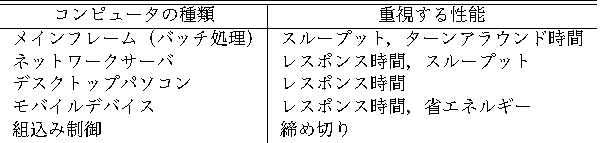
\includegraphics[scale=1.0]{Tbl/schedulingObjective.pdf}
\end{mytable}

\section{プロセスの振舞}
一般に,プロセスは計算と入出力を繰り返す.
計算と入出力にかかる時間の割合に応じて,
二種類のプロセスに分類できる.

\subsection{CPUバウンドプロセス}
例として,動画を圧縮するビデオエンコーディング・プロセスを考えてみよう.
プロセスは,\figref{cpuIoBound}(a)に示すように,次の三つの処理を繰り返す.

\begin{enumerate}
\item 未圧縮の動画ファイルを少し読む.
\item 圧縮処理を行う.
\item 結果を圧縮済み動画ファイル書込む.
\end{enumerate}

ビデオエンコーディング・プロセスはCPUが行う圧縮処理に長い時間がかかり,
入出力にかかる時間が短い.
このようにCPU処理にかかる時間が相対的に長いプロセスのことを
{\bf CPUバウンド(CPU-bound)プロセス}と呼ぶ.
また,CPUが使用される期間を{\bf CPUバースト(CPU burst)},
I/Oが使用される期間を{\bf I/Oバースト(I/O burst)}と呼ぶ.
CPUバウンドプロセスは長いCPUバーストと短いI/Oバーストを持つ.

\begin{myfig}{btp}{CPUバウンドとI/Oバウンドプロセス}{cpuIoBound}
\myincludegraphics{cpuBound-crop.pdf}{scale=0.66}
%~~~~

\vspace{0.8cm}

\myincludegraphics{ioBound-crop.pdf}{scale=0.66}
\end{myfig}

\subsection{I/Oバウンドプロセス}
二つ目の例としてスプレッドシート・プロセスを考えてみよう.
スプレッドシート・プロセスは,
まず,ユーザが何れかのセルにデータを入力するのを待つ.
次に,入力されたデータを用いてスプレッドシートの再計算を行い結果を表示する.
ユーザがセルにデータを入力するたびに同様な処理を繰り返す.
このプロセスは\figref{cpuIoBound}(b)に示すように,
ユーザ操作を待つ長い入力待ちと,
再計算と表示を行う短いCPU処理を行う.
このような,長いI/Oバーストと短いCPUバーストを持つプロセスを
{\bf I/Oバウンド(I/O-bound)プロセス}と呼ぶ.

\section{スケジューリング方式}
いくつかの代表的なスケジューリング方式を紹介する.

\subsection{First-Come, First-Served(FCFS)スケジューリング}
Ready状態になった順(到着順)に実行する方式である.
Running状態になったらブロックするまで実行を継続する.
プリエンプションはしない.
以下の例ではCPUバースト一回分の期間しか示さないが,
実際は,\figref{cpuIoBound}に示すようにCPUバースが繰り返し発生する.

FCFS方式は実行可能列をFIFOにするだけで実現できるが性能は良くない.
例えば次の三つのプロセスが時刻0で,
$P_1$,$P_2$,$P_3$の順にReady状態になったとする.

\begin{center}
\begin{tabular}{c c c}
プロセス & 到着時刻 & CPUバースト時間(ms) \\
\hline
$P_1$    & 0 & 100 \\
$P_2$    & 0 & 20 \\
$P_3$    & 0 & 10 \\
\end{tabular}
\end{center}

この時,三つのプロセスの実行開始・終了の時刻を図で表すと次のようになる.

\begin{center}
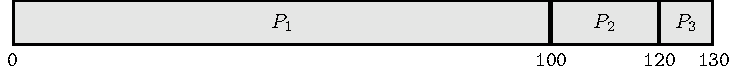
\includegraphics[scale=1.0]{GanntChart/fcfs1.pdf}
\end{center}

平均ターンアラウンド時間を計算すると,
$(100+120+130) / 3 = 117$ ms となる.
もしも,プロセスの到着順が$P_2$,$P_3$,$P_1$の順だったとすると,
三つのプロセスの実行開始・終了の時刻は図のようになる.

\begin{center}
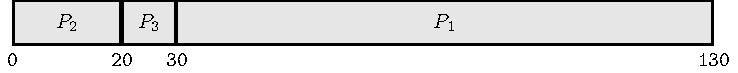
\includegraphics[scale=1.0]{GanntChart/fcfs2.pdf}
\end{center}

この場合の
平均ターンアラウンド時間を計算すると,
$(20+30+130) / 3 = 60$ ms となる.
このように,FCFSでは最悪な平均ターンアラウンド時間を選択することもある.
プリエンプションをしないので,
一旦,CPUバウンドなプロセスが実行を開始すると,
他のプロセスは長い時間待たされる.

\subsection{Shortest-Job-First(SJF)スケジューリング}
SJF方式\footnote{皆さんの教科書ではSPTのこと.}は,
平均ターンアラウンド時間を最小にするスケジューリング方式である.
SJF方式ではCPUバースト時間が短いものを先に実行するようにスケジューリングする.
実行可能列はCPUバースト時間が短い順にソートされている.

三つのプロセスがあった時,
実行順に各プロセスの実行時間が$T_1$,$T_2$,$T_3$とすると,
平均ターンアラウンド時間は,
$(T_1+(T_1+T_2)+(T_1+T_2+T_3))/3=T_1+T_2*2/3+T_1/3$となるり,
先に実行したプロセスの実行時間ほど結果に及ぼす影響が大きいことが分かる.
実行時間が短いプロセスを先に実行するスケジューリング方式は,
平均ターンアラウンド時間を最小にする.

前出の三つのプロセスをSJF方式でスケジューリングした時の,
実行開始・終了時刻は次の図のようになる.

\begin{center}
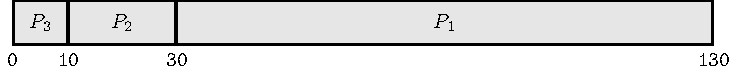
\includegraphics[scale=1.0]{GanntChart/sjf1.pdf}
\end{center}

この図より平均ターンアラウンド時間を求めると
$(10+30+130)/3 = 57$ ms となり,これまでで最短である.
しかし,次回のCPUバースト時間を知ることは一般には不可能なので,
SJF方式は現実的な方式ではない.
次回のCPUバースト時間を予測することで擬似的なSJF方式を実現する.

次回のCPUバースト時間を予測する方法として,
指数平滑平均(exponential average)を用いる例を紹介する.
次回の予測時間を$T_{n+1}$,
前回の予測時間を$T_{n}$,
前回の実際のCPUバースト時間を$t_{n}$とすると,
$0 \le \alpha \le 1$の時,
指数平滑平均は次の式で表すことができる.

\[T_{n+1} = \alpha t_n + ( 1 - \alpha ) T_n\]

この式から

\[T_{n+1} = \alpha t_n + ( 1 - \alpha ) \alpha t_{n-1} + \dots +
 ( 1 - \alpha )^j \alpha t_{n-j} + \dots + (1 - \alpha )^{n+1} T_0 \]

を得る.$\alpha = 0.5$ の場合は,

\[T_{n+1} = 0.5 t_n + 0.5^2 t_{n-1} + \dots +
0.5^{j+1} t_{n-j} + \dots + 0.5^{n+1} T_0 \]

となる.
この式は,過去のCPUバースト時間を,
最近のものほど大きな重みを付けて平均したものになっている.
つまり,次回のCPUバースト時間は,
過去のCPUバースト時間と同程度であろうとの仮定に基づいた予測値を計算している.

\subsection{Shortest-Remaining-Time-First(SRTF)スケジューリング}
SRTF方式\footnote{皆さんの教科書ではSRPTのこと.}は,
プリエンプション付きのSJF方式である.
プロセスがReady状態になるとき,
このプロセスのCPUバースト時間と
実行中のプロセスの{\bf 残りCPUバースト時間}とを比較し,
{\bf 残りCPUバースト時間}の方が長いときプリエンプションをおこす.
次の例でSJTとSRFTを比較してみよう.

\begin{center}
\begin{tabular}{c c c}
プロセス & 到着時刻 & CPUバースト時間(ms) \\
\hline
$P_1$    & 0  & 60 \\
$P_2$    & 10 & 40 \\
$P_3$    & 60 & 30 \\
\end{tabular}
\end{center}

三つのプロセスをSJFでスケジューリングした場合は次の図のようになる.

\begin{center}
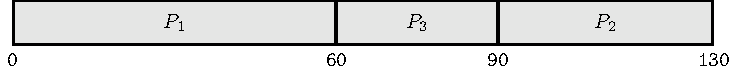
\includegraphics[scale=1.0]{GanntChart/sjf2.pdf}
\end{center}

平均ターンアラウンド時間を計算すると,
$((60-0)+(90-10)+(130-60))/3=70$ ms となる.
三つのプロセスをSRTFでスケジューリングした場合は次の図のようになる.

\begin{center}
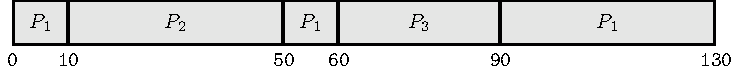
\includegraphics[scale=1.0]{GanntChart/srtf1.pdf}
\end{center}

$P_2$が到着した時,
$P_2$のCPUバースト時間($40$ ms)の方が
$P_1$の残りCPUバースト時間($60 - 10 = 50$ ms)より短いので,
$P_1$はプリエンプションし$P_2$が先に実行される.
$P_3$が到着した時も同様である.
平均ターンアラウンド時間を計算すると,
$((130-0)+(50-10)+(90-60))/3=67$ ms となり,
SJFよりも改善されている.

\subsection{Round-Robin(RR)スケジューリング}
{\bf タイムシェアリングシステム(TSS)}で使用された方式である.
{\bf クォンタム時間(time quantum)},または,
{\bf タイムスライス(time slice)}と呼ばれる10 ms 〜 100 ms 程度の
一定の時間が予め決められている.
実行可能列はFIFOになっている.
実行可能列の先頭のプロセスにCPUが割り付けられてRunning状態になる.
プロセスの実行が{\bf クォンタム時間}連続するとプリエンプションが発生し,
プロセスは実行可能列の最後尾に付け加えられる.

{\bf クォンタム時間($q$)}が短いと{\bf レスポンス時間}が短くなり,
対話的な処理が円滑に行える.
例えば,10個のプロセスがCPUを奪い合うような状況でも,
$q = 10$ ms なら$100$ ms に一度は全てのプロセスにCPUが割り付けられる.
しかし,$q$ を小さくしすぎるとコンテキストスイッチの回数が多くなり,
オーバーヘッドが大きくなる.
逆に $q$ が長いとFCFSと同じ結果になる.

前出の三つのプロセスをRR方式($q = 10$ ms)でスケジューリングした例を
次の図に示す.
なお,
新規プロセスと,
クォンタム時間を使い切りプリエンプションしたプロセスが,
同時に実行可能列に追加される場合は,
新規プロセスを優先することにする.

\begin{center}
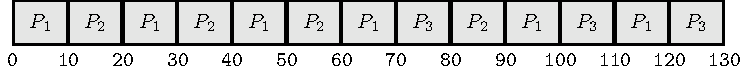
\includegraphics[scale=1.0]{GanntChart/rr1.pdf}
\end{center}

平均ターンアラウンド時間を計算すると,
$((120-0)+(90-10)+(130-60))/3=90$ ms となる.
次に $q = 50$ ms でスケジューリングした例を示す.

\begin{center}
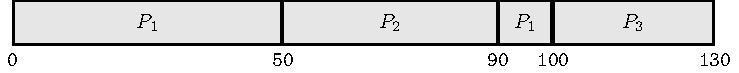
\includegraphics[scale=1.0]{GanntChart/rr2.pdf}
\end{center}

平均ターンアラウンド時間を計算すると,
$((100-0)+(90-10)+(130-60))/3=83$ ms となる.
$q = 50$ ms でスケジューリングした方が,
平均ターンアラウンド時間が短くなった上に,
コンテキストスイッチの回数が少ない.
このようなプロセスの集合に対しては,
$q = 10$ ms はクォンタム時間が短すぎると言える.

\subsection{Priority (優先度順)スケジューリング}
プロセス毎に決められた{\bf 優先度}を基に行うスケジューリング方式である.
実行中に優先度が変化する{\bf 動的優先度}を用いる方法と,
プロセス生成時に決められ変化しない{\bf 静的優先度}を用いる方法がある.
TacOSは{\bf 静的優先度}を用いる優先度順スケジューリング方式を用いる.
SRTF方式は,
次回CPUバースト時間が短い順の{\bf 動的優先度}方式と考えられる.

優先度順スケジューリング方式の問題点は,
優先度の低いプロセスが全く実行されない{\bf スタベーション(stavation)}が
発生することである.
これの対策として,
実行可能列に留まるプロセスの優先度を徐々に高くしていく
{\bf エージング(aging)}が用いられる.
実行可能列に長く留まるプロセスは優先度が高くなり,
やがて実行される.

\subsection{Multilevel Feedback Queue(FB)スケジューリング}
Windows,macOS,UNIX等で広く使用されているスケジューリング方式である.
\figref{multilevelFeedbackQueue}に示すように実行可能列を優先度別に複数設ける.
優先度が近いプロセスが同じ実行可能列に登録される.
同じ実行可能列ではRR方式でスケジューリングするので\footnote{
実行可能列ごとに,異なるスケジューリング方式を採用することも可能である.
},
列内でプロセスの順番は優先度とは関係がない.
CPUを割り付ける際は,
優先度の高い実行可能列から順に調べ,
最初に見つかった空ではない実行可能列を使用する.

\myfigure{btp}{scale=0.6}{multilevelFeedbackQueue-crop.pdf}
{Multilevel Feedback Queue}{multilevelFeedbackQueue}

プロセスの優先度は動的に変化する方式を用いる.
CPUバウンドなプロセスの優先度は急激に引き下げられ,
プロセスは下位の実行可能列に移動する.
長く実行可能列に留まっているプロセスは{\bf エージング}により
優先度が引き上げられ,上位の実行可能列に移動する.
実行中のプロセスより上位の実行可能列にプロセスが登録されると
プリエンプションが発生し,実行中のプロセスはCPUを取り上げられる.

\section{TacOSのスケジューラ}
実行可能になったプロセスをスケジューリングするプログラムを{\bf スケジューラ}と呼ぶ.
スケジューラの例として,
TacOSのスケジューラのソースプログラムを\figref{tacosSch}に示す\footnote{
\figref{tacosSch}はTacOSのソースコード
\url{https://github.com/tctsigemura/TacOS/blob/master/os/kernel/kernel.cmm}
の一部である.}.
TacOSの実行可能列は,
PCBの番兵付き重連結環状リストとして表現する
(\figref{tacosReadyQueue}参照).

\begin{figure}[btp]
\lstinputlisting{Lst/sch.cmm}
\caption{TacOSのスケジューラ・ソースプログラム}
\label{fig:tacosSch}
\end{figure}

\begin{description}
\item[1〜7行] 関数\|insProc()|は,
実行可能列にPCBを登録するために使用される.
スケジューラ以外からも呼出される汎用的なものである.

\item[9〜19行] 関数\|schProc()|がスケジューラである.
\|enice|がプロセスの優先度である.
\|enice|は値が小さい方が優先度が高い.
スケジューラは,
実行可能列(\|readyQueue|)を番兵PCBの次のPCBから開始して(14行),
挿入するプロセスの\|enice|より大きいものを探す(15,16行).
大きいものを見つけたら\|insProc()|を使用して,
見つけたPCBの直前に新しいプロセスのPCBを挿入する(17行).
実行可能列の最後には,常時IdleプロセスのPCBが置かれている
(\figref{tacosReadyQueue}参照).
Idleの\|enice|は最大値に設定されているので15行のループは必ず正常に終了する.

現在の実装では,\|enice|はプロセス生成時に\|nice|と同じ値に設定され,
その後は変化しない.
TacOSは{\bf 静的優先度}を用いる{\bf 優先度順スケジューリング方式}を用いていることになる.
将来,\|enice|の値を動的に変化させるように変更すれば,
{\bf 動的優先度}方式になる.

\|setPri()|関数はPSWの割込み許可フラグを操作するために使用している.
詳しくは「\ref{setPri} setPri()関数」で説明する.
\end{description}
 % スケジューリング
\chapter{プロセス同期}
\label{synchronaization}
これまで見てきたように,
複数のプロセス(スレッド)が並行して実行される.
複数の並行して実行されるプロセス(スレッド)が,決して競合することなく,
必要に応じて協調して動作するために,プロセス(スレッド)間で同期をとる必要がある.
この章ではプロセス(スレッド)間の同期について勉強する.

\section{競合(Race Condition, Competition)}
複数のプロセス(スレッド)が資源を共有して処理を進めることがある.
ここで言う資源とは
「スレッド間で共有する変数」,
「プロセス間で共有するメモリ」,
「カーネル内部のデータ構造」,
「ファイル」,
「入出力装置」
等が考えられる.
共有する資源をプロセス(スレッド)がアクセスする時,
きちんとした取り決めが無いと誤った結果になる場合がある.

例えば,銀行口座を管理する架空の例を考えよう.
一つのプロセス内で,
入金を処理するスレッドと,
引き落としを処理するスレッドが並行して実行されているとする.
\figref{race}にこのプロセスの処理内容の一部をTeC風のアセンブリ言語で示す.

\begin{myfig}{btp}{共有変数をアクセスする二つのスレッド}{race}
\lstinputlisting[numbers=none]{Lst/race.txt}
\end{myfig}

ほぼ同時に,プロセスが給料3万円の振込と,カード料金2万円の引き落としを受信した場合を考えてみよう.
二つのスレッドが競って\|account|変数の更新をすることになる.
処理前は\|account|変数に口座の残高10万円が記録されていたとする.

\begin{quote}
\begin{enumerate}
\item (1)→(2)→(3)→(a)→(b)→(c)の順で実行された場合 \\
\|account|変数の値は11万円になり正しい結果になる.

\item (a)→(b)→(c)→(1)→(2)→(3)の順で実行された場合 \\
\|account|変数の値は11万円になり正しい結果になる.

\item (1)→(2)→(a)→(b)→(c)→(3)の順で実行された場合 \\
入金管理スレッドが途中でpreemptionし,
引き落としスレッドが実行された後,
入金管理スレッドが再開された場合である.
\|account|変数の値は13万円になる.

\item (1)→(a)→(2)→(b)→(3)→(c)の順で実行された場合 \\
二つのCPUが並列にスレッドを実行した場合である.
\|account|変数の値は8万円になる.
\end{enumerate}
\end{quote}

以上のように,
スレッドの実行順序等により計算結果が間違ってしまうことがある.
これは資源の利用について,
{\tt 競合(Race Condition または Competition)}が発生しているからである.

\section{クリティカルセクション(Critical Section)}
\label{criticalsection}
競合が発生するのは,
一方のスレッドが自分のCPUレジスタにコピーした\|account|の値を
変更し書き戻すまでの間(変更中)に,
もう一方のスレッドが\|account|の値を
自分のCPUレジスタにコピーすることが原因である.
「変更中」の共有変数に他のスレッドがアクセスすることを禁止する必要がある.
他のスレッドが共有変数にアクセスすることが許されないプログラムの区間を
{\tt クリティカルセクション(Critical Section)},または,
{\tt クリティカルリージョン(Critical Region)}と呼ぶ.

\figref{race}の例で「(1)から(3)」と「(a)から(c)」は
\|account|変数のクリティカルセクションであり,
この区間をどれかのスレッドが実行している間は,
他のスレッドが\|account|変数にアクセスしてはならない.
クリティカルセクションの競合問題を効率よく解決するためには,
次の三つの条件を満たす必要がある.

\begin{quote}
\begin{enumerate}
\item 二つ以上のプロセス(スレッド)が同時にクリティカルセクションに入らない.
\item クリティカルセクションに入っているプロセス(スレッド)がない時は,
待たされることなくクリティカルセクションに入ることができる.
\item クリティカルセクションに入るために永遠に待たされることがない.
\end{enumerate}
\end{quote}

\section{相互排除(Mutual Exclusion)}
複数のプロセス(スレッド)が同時にクリティカルセクションに
入らないように制御することである.
{\bf 排他制御}または{\bf 相互排他}とも呼ばれる.
{\bf 相互排除}を達成するために,
プロセス(スレッド)は,
クリティカルセクションに入る際に権利を得る手続きを行う.
これを行うプログラムの部分を
{\bf エントリーセクション(Entry Section)}と呼ぶ.
クリティカルセクションを出る際に権利を返却する手続きを行う.
これを行うプログラムの部分を
{\bf エグジットセクション(Exit Section)}と呼ぶ.

\subsection{割込み禁止}
\label{disableInterrupt}
シングルプロセッサ(CPUが一つしかない)システムでは,
クリティカルセクションを実行するとき割込みを禁止することで目的を達成できる.
\figref{disableInterrupt}に\figref{race}を改良したプログラムを示す.

\begin{myfig}{btp}{割込み禁止による相互排除}{disableInterrupt}
\lstinputlisting[numbers=none]{Lst/disableInterrupt.txt}
\end{myfig}

エントリーセクションで
DI(Disable Interrrupt)命令を実行し割込みを禁止する.
エグジットセクションで
EI(Enable Interrrupt)命令を実行し割込みを許可する.
クリティカルセクションでは,
CPUが割込みを受付けない\footnote{
再度,割込みが許可されるまで保留になる.
プリエンプションはクリティカルセクションを出るまで遅延する.
}のでプリエンプションは発生しない.
クリティカルセクションの終わりまでCPUは連続して命令を実行する.
また,CPUが一つしかないので他のCPUが\|account|変数をアクセスこともない.
よって,\|account|変数の変更中に他のプロセス(スレッド)が
\|account|変数をアクセスすることはない.

この方法は簡単に相互排除を行うことができるが,
割込み禁止時間が長くならないように注意する必要がある.
割込み禁止が長くなると,
タイマーからの割込みを取りこぼし時計が正確に進まなくなったり,
入出力装置の制御が間に合わなくなるなどの弊害が生じる\footnote{
割込み禁止期間に同じ割込みが複数回発生した場合,
割込み許可になったとき割込みの種類につき一度だけ割込みが発生する.
ハードウェアに,保留になった割込みのカウンタはない.}.
また,DI命令,EI命令は特権命令なので,
カーネル内だけで使用できる手法である.

\subsection{専用命令を用いる方式}
マルチプロセッサ(CPUが複数ある)システムでは,
割込み禁止による方法では目的を達成することができない.
クリティカルセクションでプリエンプションが発生しなくても,
他のCPUによって実行されるプロセス(スレッド)がクリティカルセクションに
入る可能性があるからである.

マルチプロセッサシステムとは,
\figref{hardBlock}に示したメモリを共有するSMPシステムのことである.
複数のCPUによるメモリのアクセスはハードウェアにより順序付けされる.
同じメモリアドレスへのアクセスが競合し,
どちらのCPUが書き込んだ値とも異なる値になることはない.
順序付けの結果,後になった書き込みの結果がメモリに残る.
また機械語命令は,一部の例外を除いて,
途中で割込まれることはない.
このようなシステムでは,
以下の機械語命令を相互排除の目的に使用できる.

\begin{itemize}
\item {\bf TS(Test and Set)命令} \\
TS命令は「(1) メモリの値をCPUレジスタにロード」し,
「(2) 1を同じメモリアドレスに書き込む」命令である.
この二つを他のCPUのメモリアクセスに割込まれることなく,
{\bf アトミック(atomic)}に実行する.
TS命令(\|TS R,M|)の動作は,例えば次のようになる.

\begin{quote}
\begin{enumerate}
\item バスをロックする
\item $R \leftarrow [M]$
\item {\tt if (R==0) } $Zero \leftarrow 1;$ {\tt ~else} $Zero \leftarrow 0;$
\item $[M] \leftarrow 1$
\item バスのロックを解除する
\end{enumerate}
\end{quote}

TS命令は,他のCPUがメモリをアクセスしないように,まずバスをロックする.
次に,メモリの指定番地から値をCPUレジスタにロードする.
また,レジスタの値によってCPUの$Zero$フラグの値を決める.
更に,メモリの指定番地に「1」をストアする.
最後にバスのロックを解除する.
ロードとストアで合計二回のメモリアクセスがあるが,
バスがロックされているので,
TS命令の実行途中に他のCPUがメモリをアクセスすることはない.
\figref{testAndSet}にTS命令の使用例を示す.
JZ命令は$Zero$フラグが「1」の場合のみジャンプする.
この例のように,
クリティカルセクションに入れるようになるまでループで待つ方式を
{\bf ビジーウェイティング(Busy Waiting)}と呼ぶ.

\begin{myfig}{btp}{TS命令の使用例}{testAndSet}
\lstinputlisting[numbers=none]{Lst/testAndSet.s}
\end{myfig}

メモリのクリアは通常のST命令でできる\footnote{
通常の命令もメモリアクセスする度にバスをロックしている.}.
TS命令を用いる場合もクリティカルセクションは割込み禁止で実行する必要がある.
クリティカルセクションでのプリエンプションを避けるためである.
もしも,優先度の低いプロセス(スレッド)が
クリティカルセクション内でプリエンプションすると,
優先度の高いプロセス(スレッド)が
エントリーセクションで{\bf ビジーウェイティング}を始め
{\bf デッドロック}に陥る可能性があるからである.
%「0」をロードしたプロセス(スレッド)は,
%クリティカルセクションでプリエンプションしてはならない.
この方式も,
特権命令DI,EIを使用するのでカーネル内でしか利用できない.

\item {\bf SW(Swap)命令} \\
SW(Swap)命令もSMPシステムでの相互排除に使用できる.
「SW  R, M」は以下を{\bf アトミック(atomic)}に実行する.

\begin{quote}
\begin{enumerate}
\item バスをロックする
\item $T \leftarrow [M]$
\item $[M] \leftarrow R$
\item $R \leftarrow T$
\item バスのロックを解除する
\end{enumerate}
\end{quote}

ここで $T$ はCPU内部の一時的なレジスタ
($T$ レジスタの存在はプログラムから見えない)である.
\figref{swap}にSW命令の使用例を示す.
使用例はTS命令のものと似ているので解説は省略する.

\begin{myfig}{btp}{SW命令の使用例}{swap}
\lstinputlisting[numbers=none]{Lst/swap.s}
\end{myfig}

\item {\bf CAS(Compare And Swap)命令}\\
CAS(Compare And Swap)命令もSMPシステムでの相互排除に使用できる.
例えば「CAS  R0, R1, M」は,以下を{\bf アトミック(atomic)}に実行する.

\begin{quote}
\begin{enumerate}
\item バスをロックする
\item $T \leftarrow [M]$
\item {\tt if ($T==R0$) \{} $[M] \leftarrow R1;~ Zero \leftarrow 1;$
      {\tt \} else \{} $R0 \leftarrow T;~  Zero \leftarrow 0;$ {\tt \}}
\item バスのロックを解除する
\end{enumerate}
\end{quote}

CAS命令を用いたエントリーセクション,
エグジットセクションの作り方も,
TS命令と同様なのでここでは使用例を省略する.
CAS命令を用いると共有資源にロックを掛けない,
{\bf ロックフリー(Lock-free)}なアルゴリズムを実現できる.
前出の銀行口座を管理する架空のプロセス(\figref{race})を
CAS命令を用いて書換えた例を\figref{cas}に示す.

\begin{myfig}{btp}{CAS命令を用いた口座管理プログラムの例}{cas}
\lstinputlisting[numbers=none]{Lst/cas.txt}
\end{myfig}

処理開始時の\|account|の値をG1に保存しておく.
計算結果を格納する際に,
処理開始から\|account|の値が変化していないことを確認してから書き込む.
以前の例では,
他のプロセスが共有資源にアクセスしないように,
何らかのロックを掛けていた.
この方式はロックを掛けずに「結果を書き込む時点で判断」している.
\end{itemize}

\subsection{フラグを用いる方式}
アルゴリズムを工夫しソフトウェアだけで相互排他を実現する方式である.
中でも1981年にG. L. Peterson が発表した
{\bf Petersonのアルゴリズム(Peterson's solution)}が有名なので紹介する.
\figref{peterson}にJava風の言語で書いた例を示す.

\begin{myfig}{btp}{Petersonのアルゴリズム}{peterson}
\lstinputlisting[numbers=none]{Lst/peterson.txt}
\end{myfig}

このアルゴリズムの特徴は次の通りである.

\begin{quote}
\begin{enumerate}
\item マルチプロセッサシステムでも使用できる.
\item 2プロセス(スレッド)以上に拡張可能だが複雑になる.
\item 最近のプロセッサと相性が悪い.(out-of-order実行)
\end{enumerate}
\end{quote}

\section{セマフォ(Semaphore)}
これまでに紹介してきた相互排除は,
主に{\bf ビジーウェイティング}を用いるものであり,
待っている間もCPUを使用し続ける.
また、割込み禁止にする必要があるのでカーネル内でしか使用できない.
これらは、カーネル内で短時間で終わる相互排除のために適しているが,
長時間に渡る場合やユーザプログラムが直接使用する場合には適さない.

そこで,オペレーティングシステムが提供するより洗練された
プロセス同期機構である{\bf セマフォ}を紹介する.
なお,これまでに紹介してきた相互排除は,セマフォを実現するためにも使用される.

\subsection{概要}
{\bf セマフォ(Semaphore:腕木式信号機)}は,
1965年に E. W. Dijkstra が提案したデータ型\footnote{
C言語なら構造体を用いてセマフォ型を宣言する.
{\tt typedef struct \{ ... \} Semaphore;}
}である.
語源となった腕木式信号機は,
鉄道で使用される\figref{semaphore}のような信号機である.

\myfigure{btp}{scale=0.4}{Fig/semaphore-crop.pdf}{腕木式信号機}{semaphore}

セマフォ型の変数は内部にカウンタ\footnote{
腕木信号機の進行・停止のように二つの状態しか取らないものを
{\bf バイナリセマフォと}呼ぶ.
ここで取り上げるカウンタを持つものは{\bf カウンティングセマフォ}と呼ぶ.
カウンタの値は0以上の整数値である.
}を持ち,また,プロセスの待ち行列を作ることができる.
セマフォ型(\|Sempahore|)の変数には,
{\bf P操作({\it Proberen}:try)}と{\bf V操作({\it Verhogen}:raise)}を
行うことができる.
カーネルはP操作とV操作を,
ユーザプロセスにシステムコールとして提供したり,
カーネル内部のサービスモジュールやデバイスドライバにサブルーチンとして提供したりする.
セマフォはプロセス(スレッド)の状態を{\bf 待ち(Waiting)状態}に変える.
{\bf ビジーウェイティングでは無い}のでCPUを無駄遣いすることはない.

\begin{quote}
\begin{description}
\item[P操作(P(S))]
%クリティカルセクションのエントリーセクション等で使用できる.
セマフォ(S)の値が1以上ならセマフォの値を1減らす.
値が0ならプロセス(スレッド)を待ち(Waiting)状態にし,
セマフォの待ち行列に追加する.
アルゴリズムをC言語風に記述したものを\figref{semPV}(a)に示す.
\item[V操作(V(S))] %クリティカルセクションのエグジットセクション等で使用できる.
セマフォ(S)の待ち行列にプロセス(スレッド)がある場合は,
それらの一つを起床させる.
待っているプロセス(スレッド)が無い場合は,セマフォ(S)の値を1増やす.
アルゴリズムをC言語風に記述したものを\figref{semPV}(b)に示す.
\end{description}
\end{quote}

\begin{myfig}{btp}{セマフォのアルゴリズム}{semPV}
\small\begin{center}
\begin{minipage}{0.48\columnwidth}
\lstinputlisting[numbers=none]{Lst/semP.c}
\centerline{(a) P操作}
\end{minipage}\hspace{1em}
\begin{minipage}{0.48\columnwidth}
\lstinputlisting[numbers=none]{Lst/semV.c}
\centerline{(b) V操作}
\end{minipage}
\end{center}
\end{myfig}

\subsection{相互排除問題の解}
初期値が1のセマフォを用いて相互排除問題の解を示すことができる.
前出の架空の銀行口座管理プロセスの例を,
セマフォを用いて解決したものを\figref{semMutex}に示す.

\begin{myfig}{btp}{セマフォを用いた相互排除問題の解}{semMutex}
\lstinputlisting{Lst/semMutex.c}
\end{myfig}

1行の\|account|は相互排除が必要なスレッド間の共有変数である.
2行の\|Semaphore|型の変数\|accSem|が排他制御に使用するセマフォである.
\|accSem|は1で初期化される.
クリティカルセクションに入るスレッドは,
まず,6行か14行で\|accSem|にP操作を行う.
どちらか先にやって来たスレッドがP操作を行った時点で\|accSem|の値が0になる.

遅れてやって来たスレッドは\|accSem|の値が0の間はクリティカルセクションに
入ることができない.
先のスレッドがクリティカルセクションを出て
8行か16行で\|accSem|にV操作を行ったら,
後のスレッドがクリティカルセクションに入ることができる.

\subsection{生産者と消費者問題(Producer-Consumer Problem)の解}
生産者プログラム(スレッド)はデータを生産し有限な長さの
{\bf リングバッファ(ring buffer)}に書き込む.
消費者プログラム(スレッド)はリングバッファからデータを読み出し消費する.
この時,満杯のリングバッファに更に書き込んだり,
空のリングバッファらデータを読み出したりしないように,
プログラム(スレッド)間で歩調を合わせる(同期する)必要がある.
セマフォを用いた解を\figref{semProducerConsumer}に示す.

\begin{myfig}{btp}{セマフォを用いた生産者消費者問題の解}{semProducerConsumer}
\lstinputlisting{Lst/semProducerConsumer.c}
\end{myfig}

\begin{quote}
\begin{description}
\item [リングバッファとセマフォ]
1行の\|buffer|は大きさ\|N|のリングバッファである.
型は応用によって決まるので,リングバッファの型は仮に\|Data|型としている.
2行の\|emptySem|はリングバッファの空きスロット数を表すセマフォである.
最初は全てのスロットが空きなので初期値は\|N|である.
3行の\|fullSem|はリングバッファの使用中スロット数を表すセマフォである.
最初は全てのスロットが空きで,
使用中のスロットは無いので,初期値は\|0|にしている.

\item [生産者スレッド]
4行から始まる\|producerThread|が,
データを生産しリングバッファに書き込むスレッドである.
5行の変数\|in|はリングバッファの次回書込み位置を表すローカル変数である.
0,1,2,...,N-1,0,1,2,...の順に値が変化する.
{\bf \|in|はスレッドのローカル変数なので,相互排除をする必要がない.}

\|producerThread|は,
7行でデータを作り,
8行で空きスロット数が1以上なら\|emptySem|の値を減らして,
9行でデータをリングバッファに書き込む.
10行で\|in|の値を更新しているが,
\|in|はローカル変数なので11行より後でも良い.
11行で使用中スロット数\|fullSem|の値を増加させる.

\item [消費者スレッド]
14行から始まる\|consumerThread|は,
データをリングバッファから読み出して消費するスレッドである.
15行の変数\|out|はリングバッファの次回読出し位置を表すローカル変数である.
{\bf \|out|もスレッドのローカル変数なので,相互排除をする必要がない.}

\|consumerThread|は,
17行で空きスロット数が1以上なら\|fullSem|の値を減らして,
18行でデータをリングバッファから読み出す.
19行で\|out|の値を更新する.
20行で空きスロット数\|emptySem|の値を増加させる.
21行で読み出したデータを使用する.
\end{description}
\end{quote}

\subsection{複数生産者と複数消費者問題(Producer-Consumer Problem)の解}
前の問題で,
関数\|producerThread()|,\|consumerThread()|それぞれについて,
複数のスレッドが存在する場合を考える.
バッファに関する同期の他に,
書き込み位置(\|in|),取出し位置(\|out|)に関する排他制御が必要になる.
解を\figref{semMultiProducerConsumer}に示す.

\begin{myfig}{btp}{セマフォを用いた複数生産者・複数消費者問題の解}
{semMultiProducerConsumer}
\lstinputlisting{Lst/semMultiProducerConsumer.c}
\end{myfig}

\begin{quote}
\begin{description}
\item [リングバッファとセマフォ]
1行から3行に変更はない.

\item [生産者スレッド]
次回書き込み位置を表す\|in|変数を複数の\|procucerThread|で共有する必要がある.
\|in|変数の宣言を5行に移動し,スレッド間の共有変数に変更した.
また,\|in|変数を\|procucerThread|間で相互排除するためのセマフォ\|inSem|を
6行に追加した.

\|producerThread|では,\|in|変数の参照や書き換えを行う12行と13行が
\|in|変数に関するクリティカルセクションである.
11行と14行に\|inSem|を用いた相互排除機構を追加した.

\item [消費者スレッド]
次回読み出し位置を表す\|out|変数について,
生産者スレッドと同様な相互排除機構を追加してある.
\end{description}
\end{quote}

\subsection{リーダ・ライタ問題(Readers-Writers Problem)の解}
共有データに対して,
読み出し{\bf だけ}するリーダプロセス(スレッド)と,
読み出し書き込みの両方を行うライタプロセス(スレッド)の
二種類がある場合に,
単に資源をロックするより{\bf 並行性(concurrency)}を高くすることができる.
リーダプロセス(スレッド)は,値を読み出すだけなので,
他のリーダプロセス(スレッド)と同時に共有データをアクセしても良い.
ライタプロセス(スレッド)は,値を書換えるので,
他のライタともリーダとも同時に共有データをアクセスすることは許されない.
セマフォによる解を\figref{semReaderWriter}に示す.

\begin{myfig}{btp}{セマフォを用いたリーダ・ライタ問題の解}{semReaderWriter}
\lstinputlisting{Lst/semReaderWriter.c}
\end{myfig}

\begin{quote}
\begin{description}
\item [共有データとセマフォ]
1行の\|records|が共有データである.
2行の\|rwSem|は共有データの相互排除用のセマフォである.
これらは,全てのスレッドに関係がある.

\item [ライタスレッド]
4行の\|writerThread|は共有データを書き換えることがあるスレッドである.
書き換え途中に他のスレッドが共有データをアクセスすることを禁止するために,
\|writerThread()|は7行で\|rwSem|にロックを掛ける.
9行でロックを解除するまで,
他のライタもリーダも同時に共有データにアクセスすることはできない.
このようなロックを{\bf 排他ロック(exclusive lock)}と呼ぶ.

\item [リーダスレッド]
16行の\|readerThread|は共有資源を読むことだけする.
書き換え途中の不完全なデータを読み出さないように,
\|writerThread|と相互排除を行う必要がある.
しかし,書き換え途中以外なら,
他のリーダスレッドと同時にデータを読んでも構わない.

13行の\|cnt|変数はリーダスレッド間で共有される.
14行の\|cntSem|セマフォは\|cnt|変数の相互排除用である.
リーダスレッドはこれらを使用し,
\|records|共有データを読み出し中のリーダスレッドの数を管理する.
19行と20行,24行と25行の二箇所が,
\|cnt|変数に関するクリティカルセクションである.

19行では最初に読み出しを始めるリーダを判断し,
最初のリーダだけが代表して\|rwSem|にロックを掛ける.
二番目にやって来たリーダはロックを掛けないのでリーダ相互は排他されない.
しかし,排他ロックを用いるライタとは相互排除される.
このようなロックを{\bf 共有ロック(shred lock)}と呼ぶ.
25行で最後に読み出しを終えるリーダを判断し,
最後のリーダだけが代表して\|rwSem|のロックを解除する.
\end{description}
\end{quote}

リーダ・ライタ問題は,
共有ロックと排他ロックを使用する問題の例になっている.
共有ロックと排他ロックの考え方は,
ここに示したスレッド間の共有変数の管理だけでなく様々な場面で使用される.
例えばUNIXのシステムコールflockは,
引数に定数\|LOCK_SH|を渡すと共有ロックを,
定数\|LOCK_EX|を渡すと排他ロックをファイルに掛ける.

また,UNIXのopenシステムコールは,
引数に\|O_SHLOCK|フラグを指定すると共有ロックを,
引数に\|O_EXLOCK|フラグを指定すると排他ロックを,
ファイルのオープン時に自動的に掛ける.

\section{TacOSのセマフォ}
TacOSではプロセス同期の基本機構としてセマフォを用いる.
セマフォ機構はTacOSのマイクロカーネルが提供する.

\subsection{データ構造}
TacOSのセマフォは\figref{sem}に示す構造体である\footnote{
\url{https://github.com/tctsigemura/TacOS/blob/master/os/kernel/process.hmm}
の一部である.}.

\begin{myfig}{btp}{TacOSのセマフォ構造体}{sem}
\lstinputlisting[numbers=none]{Lst/sem.hmm}
\end{myfig}

\figref{tacosSemaphore}に
TacOSのセマフォ関連データの構造を示す.
\|semTbl|はセマフォの一覧である.
システム起動時に\|SEM_MAX|個(30個)のセマフォを準備し\|semTbl|に登録する.
\|semInUse|はセマフォが使用中かどうかを記録する論理型の配列である.
セマフォが必要になった時に,一覧の中から空きセマフォを選んで使用する.
セマフォは一覧のインデクス(セマフォ番号)で識別するので,
P操作やV操作を行う関数の引数がセマフォ番号になる.

\myfigure{btp}{scale=0.6}{Fig/tacosSemaphore-crop.pdf}
{TacOSのセマフォ関連データ構造}{tacosSemaphore}

セマフォ構造体(\|Sem|構造体型)は,
セマフォの値(\|cnt|)とプロセスの待ち行列(\|queue|)を持っている.
システム起動時に番兵PCBを使用した空の重連結環状リストが登録される.
プロセスの待ち行列の作り方は,
\figref{tacosReadyQueue}に示した実行可能列と同様である.
次に,\figref{tacosSemaphore}で表している三つのセマフォについて説明する.

\begin{quote}
\begin{description}
\item [Sem構造体(\#0)]
セマフォ一覧(\|semTbl|)の第0行に登録されている.
Sem構造体(\#0)は使用されていないSem構造体を表している.
\|semInUse|の対応する要素はFalseになっている.

\item [Sem構造体(\#1)]
値が0の時に複数のプロセスがP操作を行った状態である.
使用中なので\|semInUse|の対応する要素はTrueになっている.
P操作を行いブロックしたプロセスがセマフォの待ち行列に入っている.
プロセスは待ち行列の最後(図では右)に追加され,
待ち行列の先頭(図では左)から取り出される.
同じセマフォについて,プロセスはFCFSのスケジューリングが適用される.

\item [Sem構造体(\#29)]
V操作の結果,値が2になっている状態を表している.
使用中なので\|semInUse|の対応する要素はTrueになっている.
値が1以上の時は,待ち行列が必ず空になる.
\end{description}
\end{quote}

\subsection{使用例}
\figref{tacosSemUse}にTacOSでのセマフォの架空の使用例を示す.
これは,\figref{semMutex}の例をTacOS用に書き換えたものである.

\begin{myfig}{btp}{TacOSでのセマフォの架空の使用例}{tacosSemUse}
\lstinputlisting{Lst/tacosSemUse.cmm}
\end{myfig}

\begin{quote}
\begin{description}
\item [共有変数と相互排除用のセマフォ]
以前の例ではセマフォを\|Semaphore|型の変数として扱っていた.
今回の例では,セマフォはカーネル内部に存在し,
使用者はセマフォを番号で指定するようになっている.
そのため3行は,セマフォ変数の宣言から,番号を記憶する整数型変数の宣言に変更された.

\item [使用するセマフォの割当て]
セマフォはカーネル内部で
\figref{tacosSemaphore}に示したように管理されている.
4行のプロセスの初期化ルーチン\|initProc()|中で,
カーネルが提供する関数\|newSem()|を用いてセマフォの割当てを受ける.
\|newSem()|関数の引数はセマフォの初期値である.

\item [P操作とV操作]
TacOSで使用できるP操作関数は\|semP()|,
V操作関数は\|semV()|である.
10行,12行,18行,20行のようにセマフォ番号を引数に使用する.
\end{description}
\end{quote}

\subsection{割当}
\figref{tacosNewSem}に
TacOSカーネル内のセマフォ割当と解放ルーチンを示す\footnote{
\url{https://github.com/tctsigemura/TacOS/blob/master/os/kernel/kernel.cmm}
の一部である.}.

\begin{myfig}{btp}{TacOSのセマフォ割当て解放ルーチン}{tacosNewSem}
\lstinputlisting{Lst/tacosNewSem.cmm}
\end{myfig}

\begin{quote}
\begin{description}
\item [データ構造]
1行の\|semTbl|,2行の\|semInUse|は,
\figref{tacosSemaphore}に描かれている「セマフォ一覧」と
「使用中のセマフォ」のことである.
\|semTbl|はTacOSの起動時に「Sem構造体」や「番兵PCB」で初期化される.

\item [割込み禁止による相互排除]
5行の\|newSem()|関数が\|semTbl|から未使用のセマフォを探す.
\|newSem()|関数や後述の\|semP()|,\|semV()|関数は,
複数のプロセスから並列に呼び出され\|semTbl|や\|semInUse|をアクセスする.
これらのデータ構造はプロセス間の共有データである.
\|newSem()|関数の内部はこれら共有データのクリティカルセクションに当たるので
相互排他が必要である.
TaCはシングルプロセッサシステムなので,
\ref{disableInterrupt}で紹介した「割込み禁止による相互排除」を行う.

6行では,
現在のフラグ\footnote{CPUのPSWのフラグのこと.}の値を\|r|に保存した後,
「割込み禁止(\|DI|)」にしている.
\|setPri()|関数はフラグの値を読み出し,
同時に引数値をフラグにセットするアセンブリ言語ルーチンである\footnote{
{\tt setPri()}関数の詳細は「\ref{setPri} {\tt setPri()}関数」を参照のこと}.
\|newSem()|関数はカーネルモードで呼出すので,
実行モードが変化しないように「カーネルモード(\|KERN|)」も指定している.

7行からのループで使用されていないセマフォを探す.
割込み禁止で実行するので探索の途中でプリエンプションは発生しない.
未使用のセマフォが見つかったら12行でそれの番号を返す.

クリティカルセクションが終わるので,通常は割込みを許可するが,
\|newSem()|関数を呼出す前から割込み禁止だった場合もある.
11行では6行で保存した\|r|を用いてフラグの状態を復旧している.
もともと\|newSem()|が割込み許可状態で呼出された場合だけ割込み許可状態に戻る.

\item [エラー処理]
未使用のセマフォが見つからなかった場合は,
15行で\|panic()|関数を呼出す.
現在のTacOSではセマフォを使用できるのはカーネルとサーバプロセスだけなので,
セマフォが不足するようならオペレーティングシステムのバグである.
\|panic()|関数はエラーメッセージを表示した後,CPUを停止する.
\|panic()|関数は戻ってこないので16行は実行されない.

\item [解放ルーチン]
20行の\|freeSem()|は割当てられていたセマフォを解放する.
共有変数\|semInUse|配列の書き換えは,
単一のストア機械語命令で終了するので割込み禁止にする必要はない\footnote{
CPUが機械語命令の途中で割込みを受け付けることはない.}.
\end{description}
\end{quote}

\subsection{P操作ルーチン}
\figref{tacosSemP}にTacOSのP操作ルーチンを示す\footnote{
\url{https://github.com/tctsigemura/TacOS/blob/master/os/kernel/kernel.cmm}
の一部である.}.
P操作ルールーチンは\|semP()|関数のことである.

\begin{myfig}{btp}{TacOSのP操作ルーチン}{tacosSemP}
\lstinputlisting{Lst/tacosSemP.cmm}
\end{myfig}

\begin{quote}
\begin{description}
\item [割込み禁止による相互排除]
\|semP()|関数も,\|semInUse|や,\|semTbl|の配下のSem構造体,
PCB構造体等の共有データをアクセスするので相互排除を必要とする.
\|semP()|関数の内部は8行と21行の\|setPri()|関数を用いて,
割り込み禁止による相互排除を行っている.

\item [セマフォ番号からセマフォ構造体への変換]
9行で引数のセマフォ番号が正当なものかチェックしている.
不正なものが渡されるようならオペレーティングシステムのバグなので
\|panic()|関数を用いてシステムを停止させる.
セマフォ番号が正しい場合は,
12行で\|semTbl|配列から目的のセマフォを見つける.

\item [セマフォ値のデクリメント]
13行でセマフォの値を調べ,1以上なら14行で値を1減らす.
この場合は21行で割り込み許可フラグを復元して\|semP()|関数を終了する.

\item [Block(事象待ち)]
13行でセマフォの値を調べ,
1未満なら16行に進み現在のプロセスをブロック\footnote{
プロセスのブロック(Block:事象待ち)については,
「\ref{procState}プロセスの状態」を参照のこと.}する.
ブロックの手順は次の通りである.

\begin{enumerate}
\item \|delProc()|関数を用いて現在のプロセスを実行可能列から外す.
\item 現在のプロセスの状態を「待ち状態(\|P_WAIT|)」に変更する.
\item 現在のプロセスをセマフォの待ち行列の最後に追加する\footnote{
{\tt insProc()}関数を用いて番兵PCBの直前に挿入する.
環状リストで番兵PCBの直前は最後尾のことになる.}.
\item \|yield()|関数を呼出しCPUを解放する.
%CPUは他の実行可能なプロセスに切り換わる.
後でセマフォがV操作されプロセスが実行可能になったら,
\|yield()|関数から実行が再開される.
\end{enumerate}

なお,ここで使用している\|delProc()|は\figref{tacosSemP}の2行目で,
\|insProc()|は\figref{tacosSch}で定義されたプロセス行列の操作関数である.
\|yield()|関数は\figref{tacosDispatcher}に示したプロセス切換えプログラムである.
\end{description}
\end{quote}

\subsection{V操作ルーチン}
\figref{tacosSemV}にTacOSのV操作ルーチンを示す\footnote{
\url{https://github.com/tctsigemura/TacOS/blob/master/os/kernel/kernel.cmm}
の一部である.}.
TacOSのV操作ルーチンは\|iSemV()|と\|semV()|の二種類がある.
\|iSemV()|関数はセマフォにV操作だけ行う.
\|semV()|関数はセマフォにV操作を行った後で,プロセス切換えを試みる.
\|semV()|関数を用いると,
V操作によって実行可能になったプロセスの優先度が
現在のプロセスの優先度より高い場合に,プロセスが切り換わる.
\|iSemV()|はカーネルや割込みハンドラ等で
プリエンプションの発生を避けたい場合に使用する.

\begin{myfig}{btp}{TacOSのV操作ルーチン}{tacosSemV}
\lstinputlisting{Lst/tacosSemV.cmm}
\end{myfig}

\begin{quote}
\begin{description}
\item [割込み禁止による相互排除]
\|iSemV()|関数や\|semV()|関数も相互排除を必要とする.
\|semV()|関数は22行と26行の\|setPri()|関数を用いて,
割り込み禁止による相互排除を行っている.
\|iSemV()|関数は,呼出し側で割り込み禁止にして使用する.

\item [セマフォ番号からセマフォ構造体への変換]
3行でセマフォ番号の妥当性をチェックしてから,
7行で\|semTbl|配列から目的のセマフォを見つける.

\item [セマフォ値のインクリメント]
10行で待ち行列の状態を調べる.
番兵PCB(\|q|)と番兵直後のPCB(\|p|)が同じなら待ち行列は空である\footnote{
\figref{tacosSemaphore}の「Sem構造体(\#29)」を参照のこと.}.
待ち行列が空の場合は11行でセマフォの値を1増やし
\|false|を返り値として\|iSemv()|関数を終了する.

\item [Complete(事象完了)]
10行で待ち行列を調べ空でないなら13行に進み,
待ち行列の先頭のプロセスを起床させる.
先頭のプロセスはComplete(事象完了)\footnote{
プロセスのComplete(事象完了)については,
「\ref{procState}プロセスの状態」を参照のこと.}の状態遷移をする.
13行でセマフォの待ち行列から先頭プロセスを外し,
14行でプロセスの状態を実行可能(\|P_RUN|)に変更し,
15行でスケジューラ(\|schProc()|関数)\footnote{
スケジューラ({\tt schProc()}関数)は\figref{tacosSch}で定義されている.}
に依頼し実行可能列の適切な位置に挿入する.
この場合は\|true|を返り値として\|iSemv()|関数を終了する.

\item [プロセスの切換え]
\|semV()|関数は,
V操作により実行可能列に新しいプロセスが追加された場合
(\|iSemv()|関数がtrueで返った場合)に\|yield()|関数を呼出す.
実行可能列に現在のプロセスより優先度の高いものがあった場合,
プロセスの切換えが起こる.
\end{description}
\end{quote}

TacOSのプロセス同期機構は全てセマフォに基づいて構成される.
例えば,メッセージ通信機構もセマフォを利用して構築されている.

\subsection{setPri()関数}
\label{setPri}
割り込み禁止による相互排除で使用した\|setPri()|関数のソースプログラムを
\figref{tacosSetPri}に示す\footnote{
\url{https://github.com/tctsigemura/TacOS/blob/master/os/util/crt0.s}
の一部である.}.
\|setPri()|関数はCPUのPSWのフラグを参照・操作し,
呼出し前の割込み許可状態を保存すると同時に,新しい値に変更する.
CPUのPSWのフラグに割込許可ビットがある.

\begin{myfig}{btp}{TacOSのフラグ操作ルーチン}{tacosSetPri}
\lstinputlisting{Lst/setPri.s}
\end{myfig}

\|setPri()|関数はTaCのアセンブリ言語で記述してある.
{\tt C--}言語から\|setPri|という名前で参照されるためには,
アセンブリ言語では\|_setPri|というラベルを宣言する必要がある.
2行は\|setPri()|関数の入口になるラベルを宣言している.

{\tt C--}言語プログラムは関数引数をスタックに積んで渡す\footnote{
C言語などの言語でも関数に引数を渡す仕組みは同様である}.
3行では{\tt C--}言語が\|setPri()|関数に渡した引数をG0に読み出している.
4行で読み出した値をスタックに積み直す.

5行では現在のフラグ値をG0にコピーする.
{\tt C--}言語では関数の返り値をG0レジスタに入れて返すので\footnote{
C言語などの言語でも関数値を返す仕組みは同様である},
この値は\|setPri()|関数の返り値になる.
6行のreti機械語命令は,
スタックからフラグとPCの値を取出し,
\|setPri()|関数を呼出した場所に制御を戻す.
この時,4行でスタックに積んだ値がフラグに読み出される.

以上の仕組みで,
\|setPri()|関数は引数の値をCPUのフラグにセットすると同時に,
以前のフラグ値を呼出し側に返している.

\section{まとめ}
この章ではプロセス間の同期に関係する話題を取り上げた.
{\bf 競合}が発生しないように,
{\bf クリティカルセクション}を実行する時は,
プロセス間の{\bf 相互排除}をする必要がある.
オペレーティングシステムのカーネル内部などで,
短時間で終わるクリティカルセクションの相互排除を行う場合は,
{\bf 割込み禁止},{\bf 専用命令}と{\bf ビジーウェイティング}を
用いる方法などが使用できる.
専用命令としてTS命令,SW命令,CAS命令を紹介した.
CAS命令は{\bf ロックフリー}なアルゴリズムを実現するために使用できる.

クリティカルセクションの実行に長い時間がかかる場合は,
セマフォなどプロセスの状態遷移を伴うオペレーティングシステムの機能を使用する.
セマフォを用いた{\bf 相互排除問題}の解,
{\bf 生産者と消費者問題}の解,
{\bf 複数生産者と複数消費者問題}の解,
{\bf リーダ・ライタ問題}の解を学んだ.

また,TacOSでセマフォがどのように実現されているかを学んだ.
セマフォ機構はマイクロカーネルによって提供される.
セマフォはカウンタとPCBの待ち行列を保持する構造体として表現される.
P操作,V操作などの内部では割込み禁止による相互排除が行われていた.

\section*{練習問題}
\begin{enumerate}
\renewcommand{\labelenumi}{\tt \arabic{chapter}.\arabic{enumi}}
 \setlength{\leftskip}{1em}

\item {\bf 競合}とは何か?

\item {\bf クリティカルセクション}とは何か?

\item {\bf 相互排除}とは何か?

\item なぜ割り込みを禁止することで相互排除ができるか?

\item 割り込み禁止による相互排除がマルチプロセッサシステムでは
不十分な理由は?

\item 割り込み禁止による相互排除はクリティカルセクションの三つの条件を
満たしているか?

\item CPUが割り込み禁止になっている間に発生した割り込みはどのように
扱われるか?

\item DI命令,EI命令が特権命令でなかったら,どのような不都合が生じるか?

\item シングルプロセッサシステムにおいて,
機械語命令は{\bf アトミック(atomic)}と言えるか?

\item マルチプロセッサシステムにおいて,
機械語命令は{\bf アトミック(atomic)}と言えるか?

\item TS命令,SW命令に共通な特長は何か?

\item \figref{testAndSet}のようなビジーウェイティングは
シングルプロセッサシステムでも使用できるか?

\item セマフォを相互排除に使用する手順を説明しなさい.

\item 生産者と消費者の問題において,
二つのセマフォはどのような値に初期化されたか?\\
二つのセマフォは何の役割を持っていたか?

\item TaCをマルチプロセッサシステムに進化させた時,
「\figref{tacosSemP} TacOSのP操作ルーチン」を
どのように改造する必要があるか?({\tt Sem}構造体を変更しない場合)

\item TaCをマルチプロセッサシステムに進化させた時,
「\figref{tacosSemP} TacOSのP操作ルーチン」を
どのように改造する必要があるか?({\tt Sem}構造体も変更して良い場合)
\end{enumerate}
 % プロセス同期
\chapter{プロセス間通信}
\label{interProcessCommunication}
この章では
プロセス間通信(IPC:Inter-Process Communication)について学ぶ.
\ref{synchronaization}章で学んだ,
「生産者と消費者の問題」や「リーダ・ライタ問題」の具体的な解を得るためには,
プロセス間で情報を共有する必要がある.
プロセス間で情報を共有する代表的な機構として,
\emph{共有メモリ}と\emph{メッセージ通信}がある.
複数のプロセスが情報を共有し協調して処理を進めることで,
次のメリットが期待できる.

\begin{itemize}
\item 複数のプロセスが共通の情報へアクセスすることができる.
\item 並列処理により,処理時間の短縮が期待できる.
\item システムを見通しの良いモジュール化された構造で構築できる.
\end{itemize}

%==============================================================================
\section{共有メモリ}
共有メモリは\figref{ipcShearedMemory}に示すように,
プロセス間で同じ物理メモリを共有する方式である.
プロセス1とプロセス2は同じ物理メモリ(共有メモリ)を,
それぞれの仮想メモリ空間に貼り付けている.

\begin{myfig}{btp}{共有メモリ}{ipcShearedMemory}
  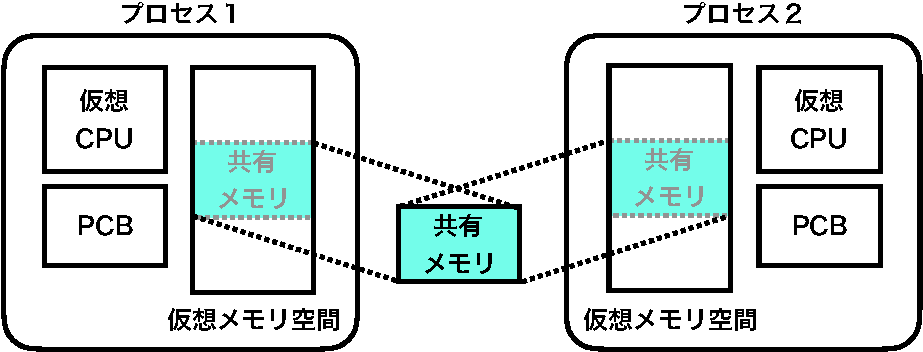
\includegraphics[scale=0.6]{Fig/ipcShearedMemory-crop.pdf}
\end{myfig}

メモリ管理のハードウェア(Memory Management Unit : MMU)\footnote{
  MMUに付いては「第\ref{memoryManagement}部 メモリ管理」で解説する.
}を適切に設定することで,
複数のプロセスの仮想メモリ空間に同じ物理メモリを貼り付ける.
メモリを貼り付ける操作はシステムコールを用いて行う.
貼り付けが完了した後は,
システムコールを用いることなく情報の共有が可能であるが,
プロセス間の同期機構は別に準備する必要がある.

\subsection{UNIXの共有メモリ関連システムコール等}
UNIXの共有メモリ関連のシステムコールとライブラリ関数を
\figref{ipcUnixSharedMemory}に紹介する.

\begin{myfig}{btp}{UNIXの共有メモリ関連システムコールとライブラリ関数}
  {ipcUnixSharedMemory}
  \lstinputlisting[numbers=none]{Lst/ipcUnixSharedMemory.txt}
\end{myfig}

\begin{quote}
  \begin{description}
  \item [\texttt{ftok()}ライブラリ関数]
    \|ftok()|は,\|path|と\|id|の組合せからから,
    システム内で一意な\|key|値を生成する.

  \item [shmgetシステムコール]
    \|key|値で識別される共有メモリセグメントのID返す.
    \|key|値で識別される共有メモリセグメントが存在しない場合は,
    \|size|バイトのものを新しく作ることも可能である.
    \|flag|の値は共有メモリのアクセス許可ビット(\|rwxrwxrwx|)と,
    \|IPC_CREAT|等のフラグである.

  \item [shmatシステムコール]
    共有メモリセグメントをID(\|shmId|)で指定し,
    プロセスの仮想アドレス空間に貼り付ける.

  \item [shmdtシステムコール]
    共有メモリセグメントをアドレス(\|addr|)で指定し,
    プロセスの仮想アドレス空間から取り除く.

  \item [shmctlシステムコール]
    共有メモリセグメントをID(\|shmId|)で指定し操作する.
    共有メモリセグメントの削除等の操作ができる.
  \end{description}
\end{quote}

\subsection{UNIXの共有メモリ使用例}
共有メモリセグメントを作成し,
そこから定期的にデータを読み出し表示するサーバプログラムの例を
リスト\ref{ipcUnixSharedMemoryServer}に示す\footnote{
  ここで示すプログラムは macOS 10.13.2 で動作確認してあるが,
  他のUNIXでも動作するはずである.}.
また,サーバプログラムが作成した共有メモリセグメントにデータを書き込む
クライアントプログラムの例を
リスト\ref{ipcUnixSharedMemoryClient}に示す.

\lstinputlisting[numbers=left,float=btp,label=ipcUnixSharedMemoryServer,
  caption=UNIXの共有メモリサーバ例]
  {SampleCode/UnixSharedMemory/ipcUnixSharedMemoryServer.c}

\lstinputlisting[numbers=left,float=btp,label=ipcUnixSharedMemoryClient,
  caption=UNIXの共有メモリクライアント例]
  {SampleCode/UnixSharedMemory/ipcUnixSharedMemoryClient.c}

サーバプログラムでは,
28行の\|printf()|が共有メモリ(\|data|)から文字列を読み出し表示する.
文字列が\|end|ならプログラムを終了する.
クライアントプログラムでは,
27行の\|fgets()|が共有メモリ(\|data|)に文字列を書き込む.
これらのプログラムでは,
共有メモリが普通の文字配列のように\|printf()|や\|fgets()|に渡されている.
共有メモリなので,
\|fgets()|が書き込んだ内容を\|printf()|が読み出すことになる.

実行例は\figref{ipcUnixSharedMemoryTest}のようになる.
図は二つのターミナルを開いて操作した状態を示している.
左半分が第一のターミナル,
右半分が第二のターミナルである.
まず,左のターミナルで
サーバプログラム(ipcUnixSharedMemoryServer)を起動する.
これで共有メモリセグメントが準備された.
次に,右のターミナルで
クライアントプログラム(ipcUnixSharedMemoryClient)を起動する.
この状態で右のターミナルに入力した文字列が,
クライアントプログラムにより共有メモリに書き込まれる.
左のターミナルで実行中のサーバプログラムは,
共有メモリの内容を定期的に表示する.

\begin{myfig}{btp}{UNIXのメモリ共有プログラム実行例}{ipcUnixSharedMemoryTest}
  \lstinputlisting[numbers=none]{Lst/ipcUnixSharedMemoryTest.txt}
\end{myfig}

ここに紹介した簡単なプログラムでは,
クライアントプロセスがデータを書き換え中に,
サーバプロセスがデータを読み出す可能性がある.
\emph{このようなプログラムを使用してはならない.}
実際に使用する場合は書き換え中のデータを読み出さないように,
セマフォ等\footnote{UNIXではセマフォも使用できる.}を
用いて相互排除を行う必要がある.
原理の確認以外の目的に,\emph{このプログラムを使用してはならない.}

%==============================================================================
\section{メッセージ通信}
メッセージ通信は\figref{ipcMessagePassing}に示すように,
システムコールを用いてプロセス間で情報をコピーする方式である.
プロセス1はsendシステムコールを用いてプロセス2へメッセージを送る.
プロセス2はreceiveシステムコールを用いてプロセス1からメッセージを受取る.
メッセージ通信は,
データを送る度にシステムコールを使用するのでオーバーヘッドが大きいが,
プロセス間の同期機構としても働く.

\begin{myfig}{btp}{メッセージ通信}{ipcMessagePassing}
  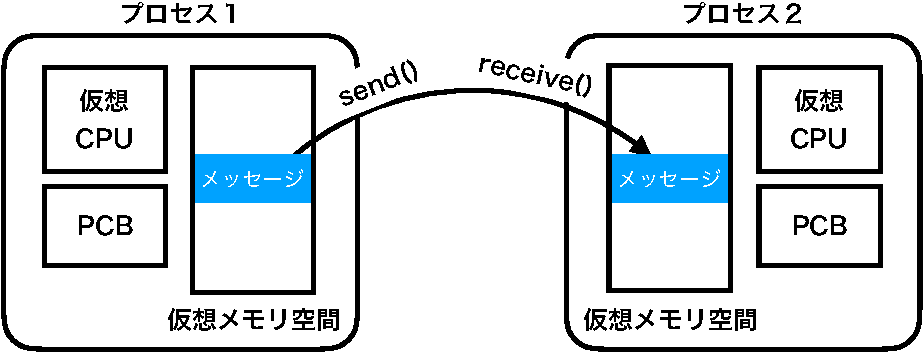
\includegraphics[scale=0.6]{Fig/ipcMessagePassing-crop.pdf}
\end{myfig}

\subsection{通信相手の指定方式(Naming)}
メッセージの通信相手を指定する方式が二つある.

\begin{quote}
  \begin{description}
  \item[直接指定方式]
    相手プロセスを直接指定する方式である.
    \figref{ipcDirect}は直接指定方式を表している.
    send,receiveシステムコールの引数は,
    \emph{相手プロセス}と\emph{メッセージ}になる.
    \emph{相手プロセス}として\|ANY|のような記述を許すことで,
    多対多の通信も可能である.
    また,受信したメッセージをいくつか貯めることが可能な,
    バッファ付きの通信方式もあり得る.
    \begin{myfig}{btp}{直接指定方式}{ipcDirect}
      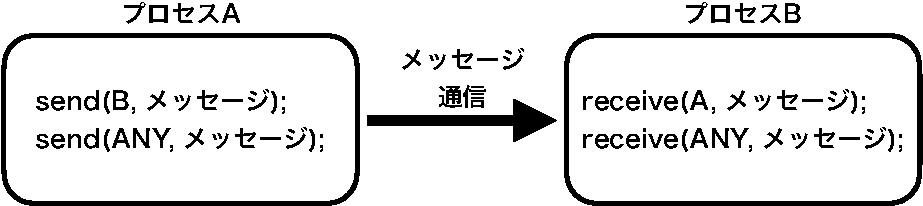
\includegraphics[scale=0.6]{Fig/ipcDirect-crop.pdf}
    \end{myfig}
  \item[間接指定方式]
    \emph{リンク(ポート,ソケット,チャネルとも呼ばれる)}を作成し,
    通信先としてリンクの名前を用いる方式である.
    \figref{ipcIndirect}は間接指定方式を表している.
    send,receiveシステムコールの引数は,
    \emph{リンク}と\emph{メッセージ}になる.
    同じリンクを共有する複数のプロセスが存在すると,
    自然に多対多の通信方式が実現できる.
    リンクにメッセージをいくつか貯めるバッファ機能を持たせる.
    %UNIXのソケットやパイプはこの方式によく似ている.
    \begin{myfig}{btp}{間接指定方式}{ipcIndirect}
      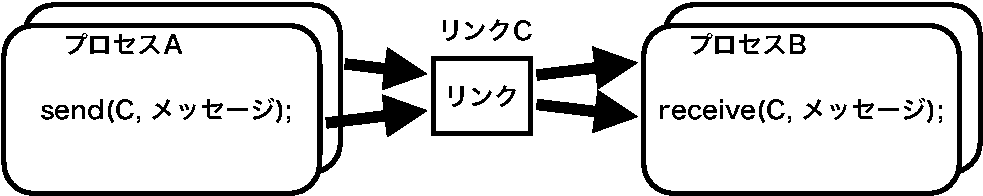
\includegraphics[scale=0.6]{Fig/ipcIndirect-crop.pdf}
    \end{myfig}
  \end{description}
\end{quote}

\subsection{バッファリング(Buffering)}
直接指定方式か間接指定方式かに関わりなく,
メッセージを格納するバッファを用意することができる.
送信プロセスはバッファに空きがあれば待ち時間なしに
sendシステムコールを完了できる.
受信プロセスはバッファにメッセージがあれば待ち時間なしに
receiveシステムコールを完了できる.

間接指定方式ではリンクがバッファを持つと考え,
リンクを作成する時点でバッファの大きさを指定する場合が多い.
\figref{ipcIndirect}で「リンク」の位置にバッファがあると考えると分かりやすい.

\subsection{メッセージの形式}
通信に用いられるメッセージの形式には次の選択肢がある.

\begin{quote}
  \begin{description}
  \item [メッセージ長] \emph{固定長方式}または\emph{可変長方式}
  \item [メッセージ形式] \emph{タグ付き}または\emph{タグなし}
  \end{description}
\end{quote}

\emph{タグ}は種類を表すためにメッセージに付加されるデータのことである.
タグ付きのメッセージ通信機構では,
送信側はメッセージにタグを付加する.
受信側はタグを指定してメッセージを選択的に受信することができる.

\subsection{同期方式(Synchronization)}
\emph{非同期方式(ノンブロッキング:Nonblocking)}と
\emph{同期方式(ブロッキング:Blocking)}の二つがある.
同期式の特別な場合としてバッファを用いない\emph{ランデブー方式}も考えられる.

\begin{quote}
  \begin{description}
  \item [非同期方式]
    \|send()|はバッファに空きがない場合エラーで終了する.
    \|receive()|はバッファにメッセージがない場合エラーで終了する.
  \item [同期方式]
    \|send()|はバッファに空きがない場合はブロックし,空きができるのを待つ.
    \|receive()|はバッファにメッセージがない場合はブロックし,
    メッセージが届くのを待つ.
  \item [ランデブー方式]
    \|send()|は受信プロセスが\|receive()|を実行するまでブロックする.
    \|receive()|は送信プロセスが\|send()|を実行するまでブロックする.
    両方のプロセスが\|send()|と\|receive()|を
    実行したらプロセス間でメッセージをコピーする.
    プロセス間で直にメッセージをコピーするので,
    バッファは不要である.
  \end{description}
\end{quote}

\subsection{UNIXのメッセージ通信システムコール}
UNIXでは複数種類のメッセージ通信機構が利用可能である.
ここでは,System V 系のUNIXを起原とする方式を紹介する.
この方式は,\emph{間接指定方式},\emph{バッファリングあり},
\emph{可変長},\emph{タグ付き}の方式である.
システムコールの引数によって,
\emph{同期方式}と\emph{非同期方式}のどちらにも対応することができる.
UNIXのメッセージ通信関連のシステムコール等を\figref{ipcUnixMessage}に示す.

\begin{myfig}{btp}{UNIXのメッセージ通信関連システムコールとデータ構造}
  {ipcUnixMessage}
  \lstinputlisting[numbers=none]{Lst/ipcUnixMessage.txt}
\end{myfig}

\begin{quote}
  \begin{description}
  \item [msgBuf構造体]
    ユーザが宣言する構造体である.
    必ず,long型の\|mtype|フィールドから始める必要がある.
    このフィールドが\emph{タグ}の役割を持つ.
    \|mtext|はメッセージの本体を格納する領域であり,
    ユーザが自由に大きさや用途を決めることができる.
  \item [msggetシステムコール]
    リンク(メッセージキューと呼ぶ)のIDを返す.
    \|key|は,共有メモリの場合と同様に\|ftok()|関数を用いて生成した値である.
    メッセージキューを識別するために用いる.
    \|msgflg|に\|IPC_CREAT|を指定すると,メッセージキューを新規に作成する.
  \item [msgsndシステムコール]
    \|msqid|で指定したメッセージキューにメッセージを送信する.
    \|msgp|に送信するメッセージを格納した\|msgBuf|構造体のポインタを渡す.
    メッセージは\emph{可変長方式}なので\|msgsz|で長さを指定する.
    \|msgsz|は構造体全体ではなく,構造体の\|mtext|部分のバイト数である.
    \|msgflg|に\|IPC_NOWAIT|フラグを指定すると\emph{非同期方式}になり,
    指定しないと\emph{同期方式}になる.
  \item [msgrcvシステムコール]
    \|msqid|で指定したメッセージキューからメッセージを受信する.
    \|msgp|に受信したメッセージを格納する\|msgBuf|構造体のポインタを渡す.
    \|msgsz|は受信可能な\|mtext|の最大バイト数である.
    \|msgtyp|に受信したいメッセージの\|mtype|を指定し,
    \emph{タグ}が合致するメッセージを選択的に受信できる.
    \|msgflg|に\|IPC_NOWAIT|フラグを指定すると\emph{非同期方式}になる.
  \item [msgctlシステムコール]
    \|msqid|で指定したメッセージキューに対して操作を行う.
    \|cmd|に操作の種類(コマンド),
    \|buf|にコマンドのパラメータを渡す.
    \|IPC_RMID|コマンドを指定するとメッセージキューの削除ができる.
  \end{description}
\end{quote}

\subsection{UNIXのメッセージ通信プログラム例}
メッセージを表現する構造体の例をリスト\ref{ipcUnixMessageH}に示す\footnote{
  ここで紹介するプログラムはmacOS 10.13.2 で動作確認した.
  macOSのオンラインマニュアルには,
  ここで紹介するメッセージ通信方式について記載がないが,
  試してみると使用できた.}.
メッセージ本体の長さは\|MAXMSG|に定義している.
以下のプログラムは,メッセージ長をこの値に固定した例になっている.

\lstinputlisting[caption=UNIXのメッセージ通信プログラム例(メッセージ構造体),
  numbers=left,float=btp,label=ipcUnixMessageH]
  {SampleCode/UnixMessage/ipcUnixMessage.h}

リスト\ref{ipcUnixMessageWriter}に
メッセージキューを作成しメッセージを書き込むプログラムの例を示す.
このプログラムは入力した文字列をメッセージ本体に格納して
メッセージキューに送信する.
タグの役割を持つ\|mtype|は常に1にしている.

\lstinputlisting[numbers=left,float=btp,label=ipcUnixMessageWriter,
  caption=UNIXのメッセージ通信プログラム例(メッセージ送信側)]
  {SampleCode/UnixMessage/ipcUnixMessageWriter.c}

リスト\ref{ipcUnixMessageReader}に,
メッセージキューからメッセージを読み込み内容を表示するプログラムの例を示す.
22行で\|msgtyp|を0にして\|msgrcv()|を実行している.
\|msgtyp|が0の場合は,
メッセージの\|mtype|(タグ)を無視して
メッセージキューの先頭から順にメッセージを受信する.
26行で\|mtype|と\|mtext|の内容を表示している.
送信側のプログラムがメッセージキューを削除すると
22行でエラーが発生し24行で終了する.

\lstinputlisting[numbers=left,float=btp,label=ipcUnixMessageReader,
  caption=UNIXのメッセージ通信プログラム例(メッセージ受信側)]
  {SampleCode/UnixMessage/ipcUnixMessageReader.c}

\subsection{UNIXのメッセージ通信プログラムの実行例}
メッセージ通信プログラムの実行例を
\figref{ipcUnixMessageTest}に示す.
図は二つのターミナルを開いて操作した状態を示している.
左半分が第一のターミナル,
右半分が第二のターミナルである.
まず,左のターミナルで送信プログラム(ipcUnixMessageWriter)を起動する.
これでメッセージキューが準備された.
次に,右のターミナルで受信プログラム(ipcUnixMessageReader)を起動する.
この状態で左のターミナルに入力した文字列が,
メッセージ通信を用いて右のターミナルで実行中のプログラムに送信される.
右のターミナルには
受信したメッセージの\|mtype|と\|mtext|の内容が表示される.

\begin{myfig}{btp}{UNIXのメッセージ通信プログラム実行例}{ipcUnixMessageTest}
  \lstinputlisting[numbers=none]{Lst/ipcUnixMessageTest.txt}
\end{myfig}

%==============================================================================
\section{メッセージ通信機構の実装例}
第\ref{tacosIPC}章に
TacOSにおけるメッセージ通信機構の実装例を紹介する.
TacOSのメッセージ通信機構はセマフォを利用して実装されている.

%==============================================================================
\section{まとめ}
この章ではプロセス間通信(IPC)について学んだ.
IPCには共有メモリとメッセージ通信の二種類があった.
UNIXの共有メモリとメッセージ通信についてプログラム例を示した.

%==============================================================================
\section*{練習問題}
\begin{enumerate}
  \renewcommand{\labelenumi}{\ttfamily\arabic{chapter}.\arabic{enumi}}
  \setlength{\leftskip}{1em}
\item 次の言葉の意味を説明しなさい.
  \begin{enumerate}
  \item 共有メモリ
  \item メッセージ通信
  \item 直接指定方式
  \item 間接指定方式
  \item バッファリング
  \item 同期方式
  \item 非同期方式
  \item ランデブー方式
  \item メッセージのタグ
  \end{enumerate}
\item プロセス間の共有メモリとスレッド間の共有変数の違いは何か?
\item UNIXの共有メモリ使用例
  (リスト\ref{ipcUnixSharedMemoryServer},
    リスト\ref{ipcUnixSharedMemoryClient})
  を実際に実行し動作確認しなさい.
  なお,ソースプログラムは以下から入手可能である. \\
  \url{\git/SampleCode/UnixSharedMemory}
\item 動作確認したプログラムでは,
  サーバプログラムは共有メモリが変更されたことを確認しないで,
  一定の時間間隔で共有メモリの内容を表示している.
  \begin{enumerate}
  \item どのような不都合が予想されるか?
  \item クライアントとサーバで同期をする方法はあるか?
  \end{enumerate}
\item メッセージ通信でバッファを大きくすることのメリットは何か?
\item UNIXのメッセージ通信プログラム例(リスト\ref{ipcUnixMessageH},
  リスト\ref{ipcUnixMessageWriter},リスト\ref{ipcUnixMessageReader})
  を実際に実行し動作確認しなさい.
  なお,ソースプログラムは以下から入手可能である. \\
  \url{\git/SampleCode/UnixMessage}
\item UNIXのメッセージ通信プログラム例は生産者と消費者の問題の解になっている.
  複数生産者と複数消費者の問題の解にもなっているか?
\item UNIXのメッセージ通信プログラム例が
  複数生産者と複数消費者の問題の解にもなっているか,
  動作確認する手順を説明しなさい.
\end{enumerate}
 % プロセス間通信
\chapter{モニタ}
\label{monitor}
複数のプロセス(スレッド)で資源を共有する際に,
プロセスの同期や相互排除にセマフォを用いることを既に学んだ.
しかし,
セマフォは基本的な機能を提供するだけで使い方はプログラマ任せなので,
間違った使用がされる可能性が高い.
その結果,
タイミングに依存した発見の難しいバグを持ったプログラムが作成される.
そこで,プログラミング言語と一体になり\footnote{
本章の話題はオペレーティングシステムではなくプログラミング言語である.},
プログラマに同期機構を強制的に利用させる仕組みが考案された.
そのような仕組みの一つとして{\bf モニタ(Monitor)}を紹介する.

\section{概要}
モニタはリソース管理用の機能と制約を持った
{\bf 抽象データ型}\cite{AbstractDataType}である.
C++やJavaなどを学んだことのある人なら,
「抽象データ型はクラスのこと」と言えば分かりやすいと思われる.

モニタは抽象データ型の一種であるが,
プロセス(スレッド)間の同期を行う機構が予め組込まれ,
その制約の下で使用するものである.
モニタの特長を以下に箇条書きにする.
% その中で,最初の二つは抽象データ型に一般的な特長である.
% 最後の一つはモニタ独特の特長である.

\begin{itemize}
\item プログラマが定義できる型である.(抽象データ型で一般的)
\item データと操作をまとめて定義する.(抽象データ型で一般的)
\item 同期のための機能が組込まれている.(モニタ独特)
\end{itemize}

なお,
Javaのクラスは同期のための機構も持っており,
一定のルールに従って使用すればモニタに近い使用もできる.
%(ただし,完全ではモニタない.)
モニタをサポートするプログラミング言語は Concurrent Pascal が有名である.

\section{構成要素}
モニタは次の要素を持つ抽象データ型である.
\figref{monitor}にモニタの模式図\footnote{
\figref{monitor}では,初期化プログラムが省略してある.}を示す.

\begin{itemize}
\item 資源(データ,変数)
\item 手続き(操作,メソッド)
\item ガード
\item 条件変数
\end{itemize}

\myfigure{btp}{scale=0.6}{Fig/monitor-crop.pdf}{モニタの模式図}{monitor}

\subsection{資源(データ,変数)}
複数のスレッドによって共有される変数のことである.
モニタの内部に必要に応じて名前付きで宣言する.
モニタの外から直接アクセスすることはできない.

\subsection{手続き(操作,メソッド)}
外部から呼び出されるプログラムである.
モニタの内部に必要に応じて名前付きで定義する.
モニタの外部から資源にアクセスできるインタフェースは手続きだけである.
手続きの実行は{\bf ガード}の働きにより排他的に行われ,
同時に実行される手続きは必ず一つ以内である.

\subsection{ガード}
モニタに一つのガードが存在し,
手続きを排他的に実行するために用いられる.
手続きを実行するときは自動的にガードにロックがかけられる.
複数のスレッドが同時にモニタに入ることはできない.
%これにより複数のスレッドが同時にモニタの手続きを実行しないようにする.

\subsection{条件変数}
モニタの内部に必要に応じて名前付きで宣言する.
条件変数にはwaitとsignalの二つの操作ができる.
wait操作を行ったスレッドは{\bf ガードを外して}条件変数の待ち行列に入る.
signal操作は条件変数の待ち行列から一つのスレッドを選んで実行可能にする.
実行可能になったスレッドは{\bf ただちに}実行を再開する.
待ち行列にスレッドが複数ある時,
どのスレッドが実行可能になるか明確な決まりはない.

\subsection{初期化プログラム}
モニタのインスタンスを作成する時に,
初期化のために実行されるプログラムである.

\section{相互排除問題の解}
前出の架空の銀行口座管理プログラムの例をモニタに置換える.
残高がスレッド間で共有される変数である.
共有変数をスレッド間で安全に共有させるためにモニタを用いる.

\subsection{共有変数の記述}
\figref{monAccount}にJava風の仮想言語による銀行口座の記述を示す.
本物の口座は他にも情報を持っているだろうが,
ここでは口座は残高だけ持っていることにする.

\begin{myfig}{btp}{モニタによる相互排除の実現(仮想言語版)}{monAccount}
\lstinputlisting[numbers=left]{Lst/MonAccount.jama}
\end{myfig}

\begin{description}
\item [2行]
この仮想言語では,Java の class 定義に似た monitor 定義ができるものとす

\item [3〜4行]
{\bf 資源}の例である.
この例では残高を表すスレッド間の共有変数({\tt money})が資源である.

\item [5〜8行]
{\bf 初期化プログラム}の例である.
モニタのインスタンス生成時に残高を引数で初期化する.

\item [9〜15行]
{\bf 手続き}の例である.
手続きは共有資源を書換えるので{\bf クリティカルセクション}であるが,
自動的に{\bf ガード}をロックし排他的に実行されるので
{\bf 明示的な相互排除を行う必要はない}.
\end{description}

\subsection{共有変数の利用}
\figref{monAccountMain}に,
\figref{monAccount}で定義した\|MonAccount|モニタを
利用した相互排除問題の解を示す.

\begin{myfig}{btp}{モニタによる相互排除の利用(仮想言語版)}{monAccountMain}
\lstinputlisting[numbers=left]{Lst/MonAccountMain.jama}
\end{myfig}

\begin{description}
\item [2行]
\figref{monAccount}に示した\|MonAccount|モニタ型のインスタンスを生成する.

\item [3〜8行]
入金管理スレッドが実行するメソッドである.
入金額を受信し口座に入金する.

\item [9〜13行]
引落し管理スレッドが実行するメソッドである.
支払い金額を受信し口座から引落す.

\item [14〜17行]
プログラムは\|main()|から実行を開始する.
\|main()|では「入金管理スレッド」と「引落し管理スレッド」を起動する.
これらのスレッドがそれぞれ,
\|receiveThread()|メソッドと\|payThread()|メソッドを実行するものとする.
\end{description}

\section{生産者と消費者問題の解}
この問題で{\bf 資源}はデータを保管するFIFO構造のバッファである.
このバッファを以下では{\bf キュー}と呼ぶことにする.
キューとキューを操作する手続きは,
全てモニタの中にまとめられる.
キューを使用するユーザプログラムには,
排他や同期に関わる難しいプログラムが含まれない.
資源の操作に関する難しいプログラムが一箇所にまとめられることも,
モニタを使用するメリットである.

以下では生産者と消費者問題の解を示すために,
まず,データのバッファになるキューをモニタを用いて記述する.
次に,キューを使用する生産者スレッドと消費者スレッド作る.

\subsection{キューの記述}
\figref{monProducerConsumer}にJava風の仮想言語によるキューの記述例を示す.
このプログラムは次のようになっている.

\begin{myfig}{btp}{モニタによるキューの実現(仮想言語版)}{monProducerConsumer}
\lstinputlisting[numbers=left]{Lst/BoundedBuffer.jama}
\end{myfig}

\begin{description}
\item [1行] この仮想言語では,
Javaの\|class|定義に似た\|monitor|定義ができるものとする.

\item [2〜5行] {\bf 資源}の例である.
キューとして使用するリングバッファのデータ構造を宣言している.
このモニタの目的は,資源であるキューを管理することである.
手続きを介すること無しに資源にアクセスすることは禁止なので,
モニタの外部からこれらのデータにアクセスできない.
\|N|がバッファの大きさ,
\|buf|がバッファ本体,
\|first|がバッファ中の次のデータ読みだし位置,
\|last|がバッファ中の次のデータ書込み位置,
\|cnt|がバッファ中のデータ件数を表す.

\item [6〜8行] {\bf 条件変数}の例である.
この仮想言語では,\|Condition|型の変数として条件変数を宣言する.
\|empty|は,
キューが空の時にデータを取り出そうとしたスレッドが,
キューにデータが書き込まれるまで待つために使用する条件変数である.
\|full|は,
キューが満杯の時にデータを書き込もうとしたスレッドが,
キューに空きができるまで待つために使用する条件変数である.

\item [9〜14行] {\bf 初期化プログラム}の例である.
モニタのインスタンスを作る際に実行されるものとする.
引数はバッファの大きさである.

\item [15〜30行] {\bf 手続き}の例である.
手続きはモニタの外部から呼び出し可能なプログラムである.
\|append()|はキューにデータを追加する.
\|remove()|はキューからデータを取り出す.
これらのプログラムが実行される時は{\bf ガード}による排他制御がされる.
次にバッファが満杯で待ちが発生する例を考えてみる.

データをキューに追加するために\|append()|を呼出したスレッドは,
コメントに\|(1)|と記された行を実行し,
キューが満杯の時17行の\|full.wait()|で待ち状態になる.
待ち状態になる時はガードを外すので,
他のスレッドがモニタに入ることができる.

他のスレッドがデータをキューから取り出すために\|remove()|を呼び出すと,
\|(2)|の行が実行され28行の\|full.signal()|まで進む.
\|full.signal()|が実行されると待ち状態のスレッドが一つ起床し,
\|(3)|の行が{\bf ただちに}実行される.
\|(3)|の実行が終了した後に(4)の行が実行される.
{\bf \|(2)|から\|(4)|の実行の間,
ガードは外さないので他のスレッドがモニタに入ることはない.}

\end{description}

\subsection{生産者と消費者スレッドの記述}
\figref{monProducerConsumerMain}に
Java風の仮想言語による生産者と消費者問題の解を示す.
このプログラムは\figref{monProducerConsumer}で定義したキューを使用する.

\begin{myfig}{btp}{モニタによる生産者と消費者問題の解(仮想言語版)}
{monProducerConsumerMain}
\lstinputlisting[numbers=left]{Lst/BoundedBufferMain.jama}
\end{myfig}

\begin{description}
\item [2行] 
\figref{monProducerConsumer}に示した
\|BoundedBuffer|モニタ型のインスタンスである.

\item [3〜8行]
生産者スレッドが実行するメソッドである.
無限にデータを生産し\|queue|に追加し続ける.

\item [9〜14行]
消費者スレッドが実行するメソッドである.
\|queue|からデータを取出し処理することを無限に繰り返す.

\item [15〜18行]
プログラムは\|main()|から実行を開始する.
\|main()|では「生産者スレッド」と「消費者スレッド」を起動する.
これらのスレッドがそれぞれ,
\|producer()|メソッドと\|consumer()|メソッドを実行する.

\end{description}

\section{セマフォによるモニタの実装}
モニタの仕組みをより正確に理解するために,
セマフォによるモニタの実装方法を考えてみる.
\figref{monProducerConsumer}の仮想言語で記述されたモニタを
Javaクラスに書換えたものを
\figref{semProducerBuffer1}と\figref{semProducerBuffer2}に示す.
モニタをサポートする言語のコンパイラは,
自動的にこのような変換を行っている.

\begin{myfig}{btp}{モニタと同等なキューをセマフォで実現(Java版,前半)}
{semProducerBuffer1}
\lstinputlisting{Lst/SemBoundedBuffer.java1}
\end{myfig}

\begin{myfig}{btp}{モニタと同等なキューをセマフォで実現(Java版,後半)}
{semProducerBuffer2}
\lstinputlisting[firstnumber=last]{Lst/SemBoundedBuffer.java2}
\end{myfig}

\subsection{モニタ機能のJavaによる実装}
\figref{semProducerBuffer1}に\|SemBoundedBuffer|クラスが
モニタと同等な動作をするために必要な機能の実装を示す.

\begin{description}
\item [1行]
\|java.util.concurrent|パッケージの\|Semaphore|クラスを使用する.
\|Semaphore|クラスはカウンティングセマフォ型である.

\item [2行]
セマフォを使用したキュークラスを\|SemBoundedBuffer|と名付ける.

\item [3行]
セマフォ(\|guard|)はモニタのガードの役割りを持っている.
スレッドは,モニタ(\|SemBoundedBuffer|クラス)内の手続き(メソッド)を実行する前に,
\|guard|をロックする.

\item [4〜5行]
モニタの条件変数に\|signal()|操作を行った時,
条件変数で待っていたスレッドがあれば{\bf ただちに}実行しなければならない.
待っていたスレッドを先に実行させるために,
\|signal()|操作を行ったスレッドを待ちにするセマフォ(\|next|)と
\|next|を待っているスレッドの数を記憶する変数(\|nextCont|)を準備する.

\item [6行]
{\bf 条件変数型}(\|Condition|)を内部クラスとして定義する.

\item [7〜8行]
条件変数にwait操作を行った時に
スレッドを待ち状態にするためのセマフォ(\|sem|)と
待っているスレッドの数をカウントする変数(\|count|)である.

\item [9行]
\|await()|は条件変数のwait操作を行うメソッドである.
Javaの\|Object|クラスに別の\|wait()|メソッドが定義さているので,
名前を\|await|にした.

\item [11〜15行]
\|release()|はセマフォにV操作を行う.
%\|Semaphore|クラスのインスタンスメソッドである.
\|nextCont|は\|signal()|中で待っているスレッドの数である.
待っているスレッドがある場合は起こす.
そうでなければモニタのガードを外す.

\item [16行]
\|acquireUninterruptibly()|はセマフォにP操作を行う.
%\|Semaphore|クラスのインスタンスメソッドである.
\|sem|は初期値0のセマフォなので,
\|await()|を呼出したスレッドがここでブロックする.

\item [19行]
条件変数にsignal操作を行うメソッドである.

\item [20〜25行]
条件変数を待っているスレッドの数(\|count|)を調べ,
1以上なら22行で起床させる.
自身は23行でブロックし,
起床したスレッドが\|exitProc()|を実行しモニタを出るのを待つ.

\item [28行]
モニタ手続きの最後の行で呼び出すメソッドである.
\|signal()|中の23行でブロックしているスレッドがあれば起床させる.
なければモニタのガードを外す.

\end{description}

\subsection{モニタ機能の使用}
\figref{semProducerBuffer2}に\|SemBoundedBuffer|クラスの後半を示す.
ここでは,\|SemBoundedBuffer|クラスの前半で定義したモニタ機能を使用している.

\begin{description}
\item [35〜38行]
{\bf 資源}(リングバッファ)を表現するための変数を宣言する.
モニタ(クラス)の外部から資源を隠蔽するために
\|private|修飾子を付けて宣言する.

\item [39〜41行]
{\bf 条件変数}は
前半で定義した\|Condition|クラスのインスタンス変数である.

\item [42〜47行]
{\bf 初期化}はクラスのコンストラクタとして実装する.

\item [48〜67行]
{\bf 手続き}は仮想言語で定義したものに,
50行と59行の「ガード取得」,
56行と65行の「手続きの出口処理」が追加されている.

\end{description}

% \section{Javaのモニタ風機構によるリーダ・ライタ問題の解}
% モニタについて理解を深めるために,
% 仮想言語によるリーダ・ライタ問題の解を示す.
% 
% \begin{myfig}{btp}{モニタによるリータ・ライタの問題(仮想言語版)}
% {monProducerConsumerMain}
% \lstinputlisting[numbers=left]{Lst/BoundedBufferMain.jama}
% \end{myfig}

\section{Javaのモニタ風機構による生産者と消費者問題の解}
Java言語はモニタに似た同期機構をサポートしている.
\figref{javaMonProducerConsumer}にJavaによる生産者と消費者問題の解を示す.
Javaには{\bf 条件変数}に相当するものが無い.

\begin{myfig}{btp}{Javaのモニタ風機構による生産者と消費者問題の解}
{javaMonProducerConsumer}
\lstinputlisting[numbers=left]{Lst/MonBoundedBuffer.java}
\end{myfig}

\begin{description}
\item [1行]
Javaのモニタ風機構を利用したキュークラスを\|MonBoundedBuffer|と名付ける.

\item [2〜5行]
{\bf 資源}(リングバッファ)を表現するための変数を宣言する.
クラスの外部から資源を隠蔽するために\|private|修飾子を付けて宣言する.

\item [6〜11行]
{\bf 初期化}をコンストラクタとして実装する.

\item [13行]
クラスの内部だけで呼び出す\|private|なメソッドである.
\|await()|メソッドは条件変数の\|wait()|に似た働きをする.

\item [14行]
\|await()|メソッドは\|Object|クラスの\|wait()|メソッドを呼び出す.
Javaオブジェクトは暗黙の条件変数が一つあるような構造になっている.
\|wait()|メソッドは暗黙の条件変数の待ち行列\footnote{
Javaでは待機セットと呼ぶ.}にスレッドを入れる.
\|wait()|メソッドは割込みなどでも終了するのでtry-catch構文で使用する.

\item [16,23行]
外部から呼び出すことができるメソッドは\|synchronized|修飾子を付けて定義する.
\|synchronized|メソッドは{\bf モニタの手続き}と同様に,
オブジェクトの{\bf ガード}をロックした\footnote{
Javaではモニタを所有すると言う.}スレッドだけが実行できる.
オブジェクトのガードをロックできない場合はガードの待ち行列に入る.

\item [17行]
バッファが満杯の場合に\|await()|を用いて暗黙の条件変数で待ち状態になる.
\|await()|は割込みなど別の理由でも終了するので,
バッファに空きができるまで繰り返し\|await()|を呼び出す.

\item [21行]
\|notify()|は暗黙の条件変数の\|signal()|に相当する.
暗黙の条件変数は一つしかないので,
スレッドが\|remove()|で待ちになっている可能性ある
(直前までバッファが空だった)場合だけ\|notify()|するようにしている.
無条件に\|notify()|を実行するようにすると,
\|append()|で複数のスレッドが待ちになっている場合に,
それらを起床させてしまう.

\item [24行]
バッファが空の場合に\|await()|を用いて暗黙の条件変数で待ち状態になる.

\item [28行]
暗黙の条件変数は一つしかないので,
スレッドが\|append()|で待ちになっている可能性ある
(直前までバッファが満杯だった)場合だけ\|notify()|するようにしている.

\item [29行]
取り出したデータを呼出し側に返す.
16行から28行の右端に書いてあるコメントは\figref{monProducerConsumer}と同様に,
生産者スレッドが17行でブロックした後,
消費者スレッドが28行で生産者スレッドを起床させるときの実行順である.
これまでの例と比較して29行が異なっている.
Javaの\|notify()|はモニタの\|signal()|と異なり,
\|synchronized|メソッドの最後まで実行した後,
スレッドの切換えが起こるからである.
\end{description}

\section{まとめ}
モニタについて学んだ.
モニタはスレッド間の同期と相互排除に使用できる
「高級言語に組込まれた仕組み」である.
モニタ内に資源と,資源を操作する手続きを記述する.
資源の相互排除と同期に関わる難しい処理が
プログラムのあちこちに分散しない.
また,モニタ内の手続き(プログラム)の実行は自動的に相互排除されるので,
クリティカルセクションを明示する必要もない.

モニタで記述した「生産者と消費者問題」の解を,
セマフォを用いて実装し直す例を示した。
この例をよく観察するとモニタの動作が細部まで理解できる.

Java言語はモニタに似た機能をサポートする言語であるが,
資源が外部からアクセスできないように\|private|修飾が必要なこと,
条件変数がないこと,
\|wait()|が\|signal()|以外でも終了すること,
\|signal()|を実行した後手続きの最後まで実行されること
等が異なる.

\section*{練習問題}
\begin{enumerate}
\renewcommand{\labelenumi}{\tt \arabic{chapter}.\arabic{enumi}}
 \setlength{\leftskip}{1em}

\item {\bf 抽象データ型}の定義を調べなさい.

\item \figref{monProducerConsumer}のプログラムにおいて,
{\tt cnt}なしにキュー(リングバッファ)を記述できるか?

\item \figref{monProducerConsumer}のプログラムにおいて,
キューが空のとき一つのスレッドが{\tt remove()}を実行した.
その後,別のスレッドが{\tt append()}を実行した.
この時の{\tt append()},{\tt remove()}内が実行される順を答えなさい.

\item \figref{monProducerConsumer}のプログラムは,
複数生産者と複数消費者問題の解に使用できるか?

\item Java風仮想言語のモニタを用いてリーダ・ライタ問題の解を示しなさい.

\item Java風仮想言語のモニタを用いてセマフォを記述しなさい.

\item {\tt semBoundedBuffer}
(\figref{semProducerBuffer1},\figref{semProducerBuffer2})に
メインルーチンを補って実際に実行しなさい.
ソースプログラムは以下から入手できる. \\
\url{https://github.com/tctsigemura/OSTextBook/blob/master/Lst/SemBoundedBuffer.java}

\item {\bf \|signal()|は手続きの最後でしか使用できないことにすると},
{\tt semBoundedBuffer}
(\figref{semProducerBuffer1},\figref{semProducerBuffer2})は
どのように簡略化できるか.

\item {\tt MonBoundedBuffer}(\figref{javaMonProducerConsumer})に
メインルーチンを補って実際に実行しなさい.
ソースプログラムは以下から入手できる.\\
\url{https://github.com/tctsigemura/OSTextBook/blob/master/Lst/MonBoundedBuffer.java}

\item \figref{monProducerConsumer}のプログラムと,
\figref{javaMonProducerConsumer}でコメントに示すように実行順序が異なる.
Javaのモニタ風機構と従来のモニタのどのような違いによるものか?

\item その他に従来のモニタとJavaのモニタ風機構の違いは何があるか?

\item モニタの signal と、セマフォのV操作の違いは何があるか?
\end{enumerate}
 % モニタ

\part{メモリ管理}
\label{memoryManagement}
\chapter{主記憶(メモリ)}
コンピュータシステムにおいて,
主記憶(メモリ)\footnote{
  本章で「主記憶」と「メモリ」は同じ意味で用いられる.
}はCPUと同様に重要な装置である.
CPUを仮想化し複数のプロセスを同時に実行可能にするには,
主記憶も管理し複数のプロセスに適切に主記憶が割り振られ,
かつ,プロセス同士が干渉しないように分離する必要がある.
この章では主記憶と主記憶管理の基本的なアイデアについて学ぶ.

%==============================================================================
\section{ハードウェア構成}
主記憶はCPUがプログラムを実行する際に,
プログラムの機械語やデータ,スタック領域等を置くメモリのことである.
TeCの主記憶は256バイトのRAM領域であったし,
4年生の実験で使用したH8/3664では32KiBのROMと2KiBのRAMであった.
現代のPCなら4GiBから16GiB程度の大きさを持つ「メモリ」のことである.

本書で前提とする
コンピュタのハードウェア構成は\figref{hardBlock}に示した.
この章ではCPUとメモリに着目するので,
図を単純化し\figref{cpuMemory}のようなモデルを用いる.
この図はCPUがアドレスを指定してメモリのデータを読み書きすることを表している.

\begin{myfig}{btp}{CPUとメモリの関係を表す単純なモデル}{cpuAndMemory}
  \begin{minipage}{0.49\columnwidth}
    \begin{center}
      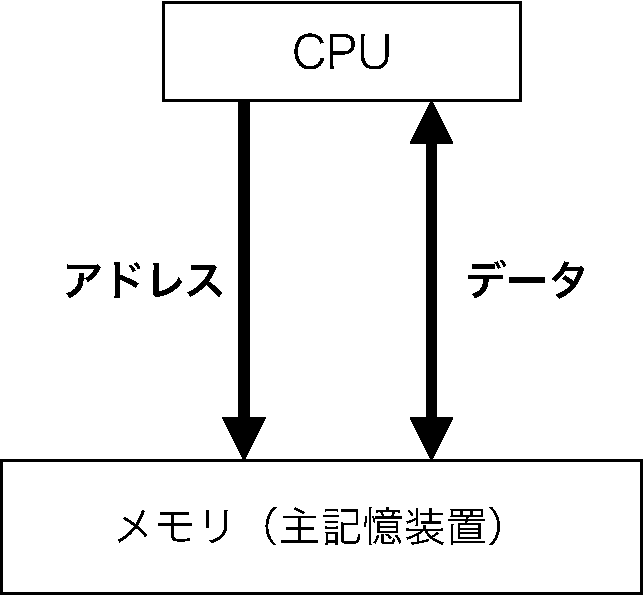
\includegraphics[scale=0.4]{Fig/cpuMemory-crop.pdf}
      \subcaption{単純なモデル}
      \label{fig:cpuMemory}
    \end{center}
  \end{minipage}
  \begin{minipage}{0.49\columnwidth}
    \begin{center}
      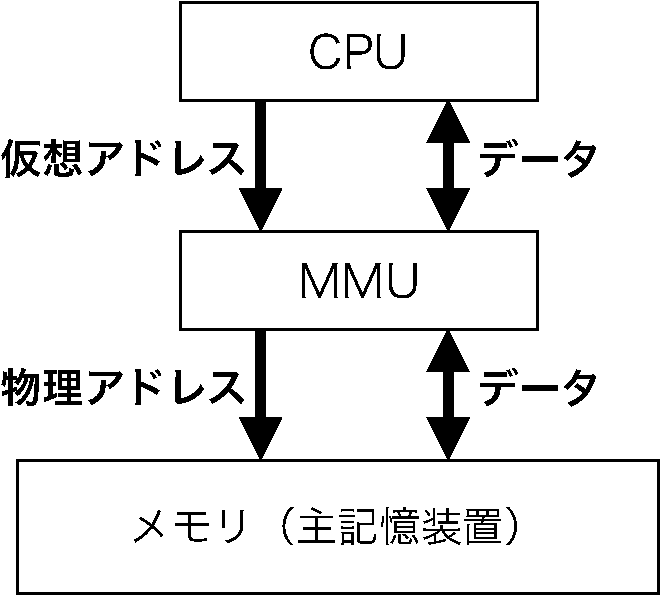
\includegraphics[scale=0.4]{Fig/cpuMmuMemory-crop.pdf}
      \subcaption{仮想化が可能なモデル}
      \label{fig:cpuMmuMemory}
    \end{center}
  \end{minipage}
\end{myfig}

プログラム実行時にCPUは以下のようにメモリをアクセスする.
\begin{enumerate}
\item 命令フェッチ(fetch)\\
  PCの値をアドレスとして出力し主記憶からデータ(命令コード)を\emph{読む}.
\item 命令デコード(decode) \\
  フェッチした命令の種類を調べる.
\item 命令実行(execution)\\
  命令を実行する際に必要に応じてデータのアドレス
  (実効アドレス:Effective Address(EA))を出力し
  主記憶のデータを\emph{読み書きする}.
\end{enumerate}

\figref{cpuMemory}のモデルは,
TeCやH8/3664のようなマイクロコンピュータの様子を表すためには十分である.
しかし,この単純なモデルでは現代の本格的なオペレーティングシステムを
作動させるには次の点で不十分である.
\begin{enumerate}
\item メモリ保護機構がない.\\
  ユーザプロセスがOSのカーネルや,
  他のプロセスを破壊することを防ぐことができない.
\item メモリの再配置機構がない.\\
  同時に複数のプロセスが主記憶にロードされる環境では,
  プロセスの起動と終了が繰り返されるうちに使用できない
  小さなメモリの断片(フラグメント)ができる.
  フラグメントを解消するために,
  実行中プロセスをメモリ内で移動する機能が必要である.
\item 仮想記憶機構が実現できない.\\
  メモリより大きなプログラムを実行するために,
  仮想記憶機構を導入したいができない.
\end{enumerate}

そこで,\figref{cpuMmuMemory}のモデルを用いる.
CPUとメモリの間に
\emph{MMU(Memory Management Unit:メモリ管理装置)}を追加する.
MMUはCPUが出力した\emph{仮想アドレス}をOSが指示したルールに則り
\emph{物理アドレス}に変換してメモリに送るハードウェアである.
\emph{OSの主記憶管理プログラムがMMUを制御することによって,
  使いやすく安全な仮想の主記憶をプロセスに提供する.}

%==============================================================================
\section{メモリ保護機構}
CPUを仮想化したことによって,
複数のユーザプロセスをメモリに同時にロードし並列実行することが可能になった.
これにより,CPUの使用効率が良くなるだけでなく,
コンピュータの使い勝手が非常に良くなった.
しかし,ユーザプログラムのバグや悪意によって,
OSカーネルや他のユーザプログラムが破壊される可能性がでてきた.
OSカーネルはそれの性質上全てのメモリ領域にアクセスする必要がある.
一方でユーザプロセスは自身に割当てられたメモリ以外に
アクセスできない仕組みが必要である.

\subsection{上限・下限レジスタ}
プロセスがアクセスしても良いメモリのアドレスの範囲をレジスタに設定し,
メモリアクセスする度にCPUが出力するアドレスとレジスタの値を比較する.
\figref{baseLimitAddrSpace}はプロセス2が実行中の
上限・下限レジスタの状態を表している.
\figref{baseLimitHardware}はアドレスを比較するハードウェアの
構成を示している.

\begin{myfig}{btp}{上限・下限レジスタの仕組み}{baseLimitRegister}
  \begin{minipage}{0.49\columnwidth}
    \begin{center}
      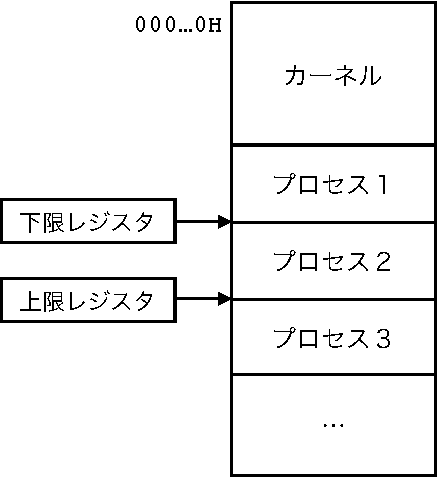
\includegraphics[scale=0.6]{Fig/baseLimitAddrSpace-crop.pdf}
      \subcaption{物理アドレス空間}
      \label{fig:baseLimitAddrSpace}
    \end{center}
  \end{minipage}
  \begin{minipage}{0.49\columnwidth}
    \begin{center}
      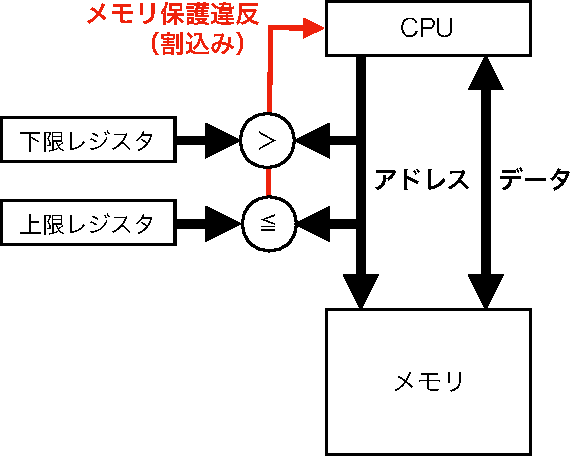
\includegraphics[scale=0.6]{Fig/baseLimitHardware-crop.pdf}
      \subcaption{ハードウェア構成}
      \label{fig:baseLimitHardware}
    \end{center}
  \end{minipage}
\end{myfig}

\begin{enumerate}
\item OSカーネルはプロセスの実行を開始する前に,
  プロセスの上限ドレスと下限ドレスを上限・下限レジスタに設定する.
  上限・下限レジスタを操作できるのはカーネルモード\footnote{
    実行モードは\ref{gen2nd}で紹介したので忘れた人は再確認すること.}で
  実行されるカーネルだけである.
  ユーザプロセスが自身のアクセスできる領域を変更することはできない.
\item カーネルはプロセスの実行を開始させる.
\item プロセスはユーザモードで実行される.
  ユーザモードで実行中は
  ハードウェアがCPUの出力するアドレスを上限・下限レジスタと比較する.
\item 上限・下限アドレスの範囲外へのアクセスの場合,
  ハードウェアがメモリアクセスを阻止しCPUに割込みをかける.
\item 割込みが発生するとユーザプロセスの実行が打ち切られ,
  制御がカーネルに移る.
\end{enumerate}

\subsection{ロック/キー機構}
主記憶をページに分割しページ毎にアクセス許可情報を持たせる.
64KiBのメモリを256ページに分割した例を\figref{lockKeyAddrSpace}に示す.
16bitのアドレスはページ番号を表す上位8bitと,
ページ内オフセットを表す下位8bitに分割される.

\figref{lockKeyHardware}に示すようにCPUは,
アドレス,アクセスキー,R/W/XをMMUに出力する.
アクセスキーはプロセス毎に決まる数字\footnote{プロセス番号でも良い.},
R/W/Xはメモリアクセスの種類を表す次のどれかである.
R(Read)は読み込みを,W(Write)書き込みを,
X(eXecute)は命令のフェッチを意味する.

MMUは許可情報表を内蔵している.
MMUはCPUが出力したアドレスからページ番号を求め表を引く.
表のプロテクションキーがアクセスキーと一致していない場合,
または,CPUのR/W/Xが表のアクセスモードに含まれていない場合は
メモリ保護違反の割込みを発生する.
MMUを操作できるのはCPUの実行モードがカーネルモードの時だけ,
MMUがメモリ保護違反の割込みを発生するのはユーザモード時だけである.

\begin{myfig}{btp}{ロック/キー機構の仕組み}{lockKey}
  \begin{minipage}{0.49\columnwidth}
    \begin{center}
      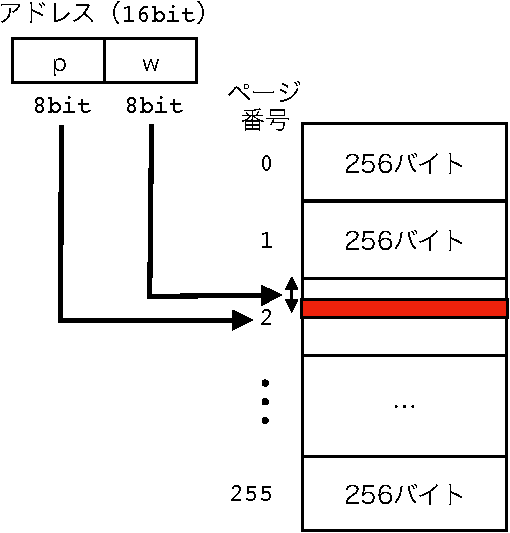
\includegraphics[scale=0.66]{Fig/lockKeyAddrSpace-crop.pdf}
      \subcaption{アドレス空間}
      \label{fig:lockKeyAddrSpace}
    \end{center}
  \end{minipage}
  \begin{minipage}{0.49\columnwidth}
    \begin{center}
      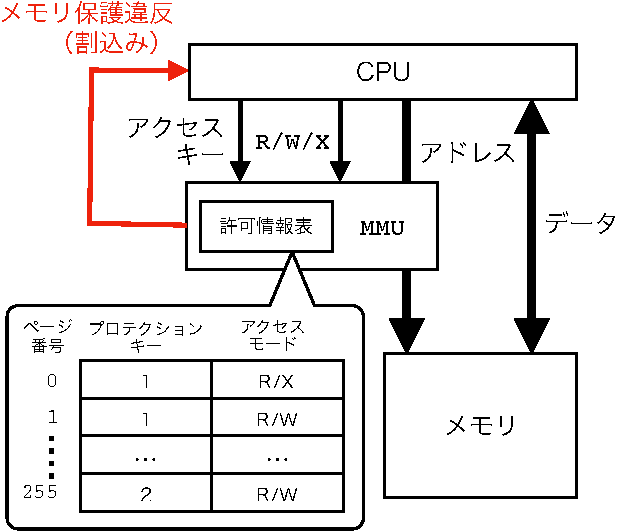
\includegraphics[scale=0.66]{Fig/lockKeyHardware-crop.pdf}
      \subcaption{ハードウェア構成}
      \label{fig:lockKeyHardware}
    \end{center}
  \end{minipage}
\end{myfig}

特別なプロテクションキー(例えば0)のページは
全てのプロセスがアクセス可能とすれば,
プロセス間の共有メモリを実現できる.

%==============================================================================
\section{プログラムの再配置}
コンパイルされたプログラムはメモリにロードされる時にアドレスが確定する.
ファイルに格納された実行可能形式プログラムは,
ロード時にアドレスを変更できる必要がある.

また,実行途中のプログラムのアドレスを変更することがある.
\figref{memoryCompaction}のようにメモリが多くの領域に分断され,
領域の間に小さなメモリの断片(\emph{メモリフラグメント})が沢山できた場合は,
プログラムの詰め合わせ(\emph{メモリコンパクション})を行う.
実行途中のプログラムを移動することを\emph{動的再配置}と呼ぶ.

\begin{myfig}{btp}{プログラムの動的再配置}{memoryCompaction}
  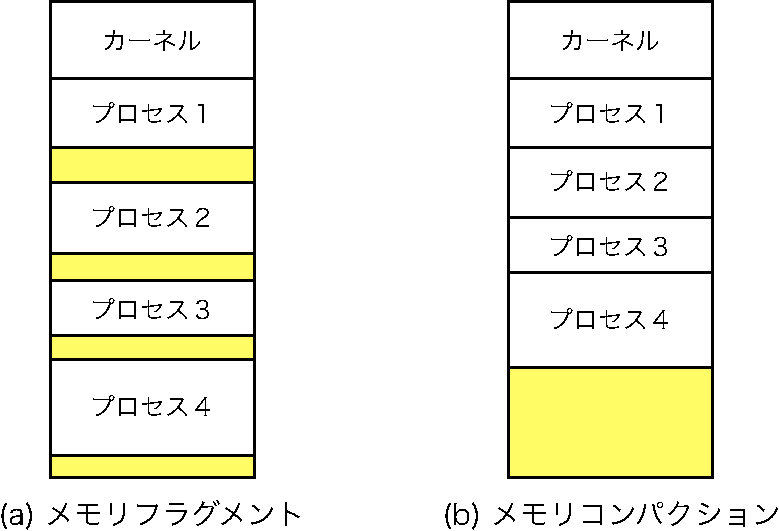
\includegraphics[scale=0.60]{Fig/memoryCompaction-crop.pdf}
\end{myfig}

\subsection{再配置可能オブジェクトファイル}
プログラミング言語で記述されたプログラムは,
コンパイルされ実行可能な機械語ファイルに変換される.
しかしコンパイル時には,
プログラムがメモリの何番地にロードされるか分からない.
そこで,
実行可能形式の機械語プログラムはジャンプ先アドレスや,
データアドレスの確定をロード時に行うことができなければならない.

ロードアドレスが確定しおらず,アドレスを変更可能な機械語プログラムは
\emph{再配置可能オブジェクト(relocatable object)}と呼ばれる.
再配置可能オブジェクトファイルは,
コンパイル済みの機械語プログラムの他に,
ファイル中のどの部分がアドレスであるかを記録した\emph{再配置表}も含む.
プログラムを主記憶にロードする際に再配置表を参照し,
プログラムやデータ中の全てのアドレス情報にロードアドレスを足し込む必要がある.
例えばプログラムを\|1234H|番地にロードすると,
\|JMP 0100H|の機械語は\|JMP 1334H|に書換える必要がある.
ロード時にアドレスを変換する方式を\emph{静的再配置}と呼ぶ.
再配置可能オブジェクトファイルの例としてTacOSが使用する
ファイルのフォーマットを付録\ref{appTacosFileFormat}に示す.

\subsection{リロケーションレジスタ}
動的再配置を行うためには,
実行中のプログラムがどこにアドレスを記憶しているか全て管理する必要がある.
しかし,CPUレジスタやスタックに書き込まれたアドレス,
リスト構造に含まれるポインタ等,
すべてのアドレスデータを追跡することは困難である.

動的再配置を可能にするための一つのアイデアは,
\emph{リロケーションレジスタ}と呼ばれる特別なハードウェアを用いることである.
\figref{relocationAddrSpace}に示すように\footnote{
  図はプロセス2を実行するための設定を表している}
リロケーションレジスタは,
プロセスのロードアドレス(B:Base)と大きさ(L:Limit)を記録するレジスタである.
ディスパッチャがプロセスを実行する時に値を設定する.

\figref{relocationHardware}に示すように
CPUが出力したアドレスはプロセスの大きさ(L)と比較される.
アドレスがL以上の場合はプロセス領域外のアドレスになるので
メモリ保護違反の割込みを発生する.
CPUのアドレスにプロセスのロードアドレス(B)を足した値がメモリアドレスになる.

\begin{myfig}{btp}{リロケーションレジスタ}{relocationRegister}
  \begin{minipage}{0.49\columnwidth}
    \begin{center}
      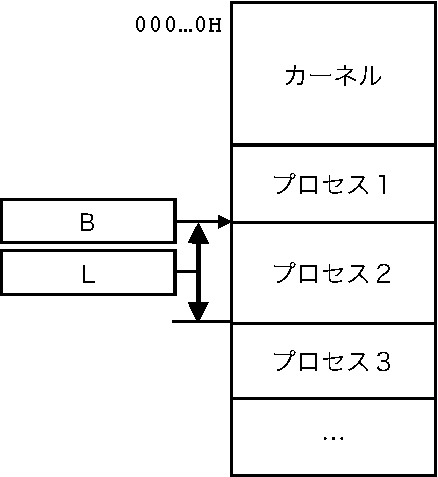
\includegraphics[scale=0.6]{Fig/relocationAddrSpace-crop.pdf}
      \subcaption{物理アドレス空間}
      \label{fig:relocationAddrSpace}
    \end{center}
  \end{minipage}
  \begin{minipage}{0.49\columnwidth}
    \begin{center}
      \includegraphics[scale=0.6]{Fig/relocationHardware-crop.pdf}
      \subcaption{ハードウェア構成}
      \label{fig:relocationHardware}
    \end{center}
  \end{minipage}
\end{myfig}

動的再配置を行うにはプロセスがRunning以外の状態の時に,
主記憶上でプロセスのメモリ領域を新しい領域にコピーする.
次回プロセスが実行される時,
ディスパッチャは新しい領域のアドレスをBにロードする.
ユーザプログラムは再配置されたことを知る必要はない.
しかし,プロセスの領域の移動は大量のメモリコピーを伴うので,
\emph{オーバーヘッドが大きい}処理である.

%==============================================================================
\section{アドレス空間の仮想化}
\figref{procOrganization}で示したように,
プロセスは各々が専用の\emph{仮想アドレス空間}(仮想メモリ空間)を持つ.
仮想アドレス空間は仮想アドレスで番地付けされている.
それに対しハードウェアとしてのメモリはシステム全体で一つしかない.
ハードウェアメモリは物理アドレスで番地付けされており,
\emph{物理アドレス空間}を形成する.
\figref{memorySpaceMapping}にプロセスの仮想アドレス空間が,
物理アドレス空間にマッピングされる様子を示す.
マッピングは,MMUよる仮想アドレスから物理アドレスへの変換によってなされる.

\begin{myfig}{btp}{仮想アドレス空間から物理アドレス空間へのマッピング}
  {memorySpaceMapping}
  \includegraphics[scale=0.60]{Fig/memorySpaceMapping-crop.pdf}
\end{myfig}

\subsection{単一仮想記憶}
多重仮想記憶に移行する中間的な形式である.
プロセスの仮想アドレスと物理アドレスが同じ方式である.
メリットが少ないので通常は次に紹介する多重仮想記憶を用いる.

\subsection{多重仮想記憶}
アドレス空間が仮想化されることにより,
全てのプロセスが0番地から始まるアドレス空間を持つことが可能になる.
プロセス毎に完全に独立したアドレス空間を持つ方式を\emph{多重仮想記憶}と呼ぶ.
実行可能形式のプログラムは,いつも0番地にロードされ実行される.
%再配置可能なオブジェクトでなくても良い.

\subsection{仮想アドレス空間の配置}
仮想アドレス空間にプログラムや変数を配置する方法は
オペレーティングシステムの種類により一定ではない.
\figref{memoryMapVsClang}とリスト\ref{cmmSample}に
UNIX上でC言語プログラムが配置される様子を示す.

\begin{myfig}{btp}{仮想アドレス空間の配置例}{memoryMapVsClang}
  \includegraphics[scale=0.6]{Fig/memoryMapVsClang-crop.pdf}
\end{myfig}

\begin{itemize}
\item 初期化済みのグローバル変数\footnote{
  正確には初期化済みの静的な変数.
  関数内で\texttt{static}修飾した変数も含まれる.}は,
  初期化データ領域(\emph{dataセグメント})に配置される.
\item 初期化されないグローバル変数\footnote{
  正確には初期化されない静的な変数.
  関数内で\texttt{static}修飾した変数も含まれる.}は,
  非初期化データ領域(\emph{bssセグメント})に配置される.
\item \texttt{main()}関数は機械語に変換され,
  プログラム領域(\emph{textセグメント})に配置される.
\item 関数のローカル変数\footnote{
  正確には自動変数.
  関数内で\texttt{static}修飾した変数は含まれない.}は,
  関数の実行開始時に\emph{スタック}または\emph{CPUレジスタ}に割り付けられ,
  関数を終了する時に破棄される.
  同じスタックを関数呼出しのために CALL 機械語命令も使用する.
  スタックは,必要に応じて仮想アドレス空間を0番地側に伸びていく.
\item \|malloc()|関数等を用いて動的に領域を割り当てると
  \emph{ヒープ}が使用される.
  ヒープは必要に応じて仮想アドレス空間を0番地とは逆の方向に伸びていく.
\end{itemize}

\lstinputlisting[caption=C言語プログラムをTaCの機械語に変換した例,
  numbers=none,float=btp,label=cmmSample]{Lst/cmmSample.s}
 % 主記憶
\chapter{メモリ割付け方式}
プロセスが実行を開始する前に,
物理メモリの一部をプロセスに割付け,
プログラムをロードする.
物理メモリを複数のプロセスで分割し利用するために,
幾つかの方式が考案されてきた.
ここでは,固定分割方式と可変分割方式について解説する.

%==============================================================================
\section{固定区画方式}
予めメモリを大小数種類の区画に分割しておく.
プロセスのサイズにより適切な区画を選択し利用する.
その様子を\figref{fixedPartition}に示す.

\begin{myfig}{btp}{固定区画方式}{fixedPartition}
  \begin{minipage}{0.49\columnwidth}
    \begin{center}
      \includegraphics[scale=0.6]{Fig/fixedPartitionLoad-crop.pdf}
      \subcaption{区画を選択しプロセスをロード}
      \label{fig:fixedParthtionA}
    \end{center}
  \end{minipage}
  \begin{minipage}{0.49\columnwidth}
    \begin{center}
      \includegraphics[scale=0.6]{Fig/fixedPartitionExec-crop.pdf}
      \subcaption{プロセスを実行}
      \label{fig:fixedParthtionB}
    \end{center}
  \end{minipage}
\end{myfig}

\figref{fixedPartition}の例では
利用可能なメモリは予め五つの区画に分割されている.
プロセス1から4を実行したい時,
ロード可能な区画を選択しロードする.
プロセス4はロード可能な区画が無いので実行できない.

区画の大きさとプロセスの大きさは一致するとは限らない.
一致しない場合は区画1から3ように,
内部に使用されない領域(\emph{内部フラグメント})が生じる.
区画4と区画5を合わせるとプロセス4をロード可能であるが,
固定区画方式では組合せて利用することはできない.
仕組みが簡単だがメモリの利用率が低い.
特徴を以下にまとめる.

\begin{enumerate}
\item 空き領域の管理が容易である.
\item 領域内部に無駄な領域(\emph{内部フラグメント})が生じる.
\item 小さな領域が複数空いていても大きなプロセスは実行できない.
\item 実行可能なプロセスのサイズに強い制約がある.\\
  (図の例では,151KiBのプロセスは実行できない.)
\item 同時に実行できるプロセスの数に制約がある.\\
  (図の例では,同時に五つ以上のプロセスは実行できない.)
\end{enumerate}

%==============================================================================
\section{可変区画方式}
メモリの空き領域から,
プロセスのサイズに合わせたメモリ区画を割付ける方式である.
\figref{variablePartition}に模式図を示す.

\begin{myfig}{btp}{可変区画方式}{variablePartition}
  \includegraphics[scale=0.6]{Fig/variablePartition-crop.pdf}
\end{myfig}

\begin{enumerate}
\item[(a)] \emph{初期状態} \\
  メモリはカーネルと,大きな単一の空き領域に分割される.
\item[(b)] \emph{実行開始} \\
  \figref{fixedPartition}と同じ四つのプロセスがロードされ実行を開始した.
  \figref{fixedPartition}の例では実行できなかった「プロセス4」も実行できる.
         (メモリの利用効率は良い.)
\item[(c)] \emph{プロセス1(P1)終了} \\
  終了したプロセスが利用していた領域は,
  再利用可能な空き領域になる.
\item[(d)] \emph{プロセス5(P5),プロセス6(P6)実行開始} \\
  120KiBの空き領域は,
  「110KiBの領域」と「10KiBの空き領域」に分割する.
  100KiBの空き領域は,
  「80KiBの領域」と「20KiBの空き領域」に分割する.
  プロセス5とプロセス6を新しい領域にロードし実行する.
\item[(e)] \emph{プロセス3(P3)終了} \\
  プロセス3が利用していた領域は,
  再利用可能な40KiB空き領域になる.
  メモリ全体では,10KiB,40KiB,20KiBの空き領域ができている.
\end{enumerate}

以上のように可変区画方式では,
プロセスの開始と終了が繰り返されるに従い小さな空き領域ができる.
このような区画の外にできる小さなメモリ領域を\emph{外部フラグメント}と呼ぶ.

%==============================================================================
\section{可変区画方式の空き領域選択方式}
以下の三つの方式が知られている.
\figref{firstBestWorstFit}に三つの方式で選択される空き領域の例を示す.

\begin{myfig}{btp}{空き領域の選択方式}{firstBestWorstFit}
  \includegraphics[scale=0.6]{Fig/firstBestWorstFit-crop.pdf}
\end{myfig}

\begin{itemize}
\item \emph{ファーストフィット(first-fit)方式}\\
  アドレス順に空き領域を探索し,
  最初に見つかった十分な大きさの領域を選択する.
\item \emph{ベストフィット(best-fit)方式}\\
  プロセスを格納可能な領域の中で最小のものを選択する.
\item \emph{ワーストフィット(worstfit)方式}\\
  最も大きな領域を選択する.
\end{itemize}

シミュレーションの結果メモリ利用率の点で,
ワーストフィット方式は最も性能が劣るが,
ファーストフィットとベストフィットの性能は互角だと言われている.
しかし実行時間の点で,
ファーストフィットがベストフィットより
優れていると言われている\cite{MemoryAllocation}.

%==============================================================================
\section{空き領域の管理方式}
プロセスによって使用中のメモリ区画は
プロセスのPCB等に記録しおけば見失う心配はない.
しかし,
どのプロセスにも属さない空き領域はメモリ管理側で記録しておく必要がある.

\begin{itemize}
\item \emph{ビットマップ(bitmap)方式}\\
  \figref{bitMap}のようにメモリを一定の大きさのブロックに分割し,
  1ブロックをビットマップの1ビットに対応させる.
  ビットが 0 ならブロックが空き状態,
  ビットが 1 なら使用中の意味になる.
  % 後で述べるページング方式において,
  % 空きページを管理するにはこの方式が適している.

  \begin{myfig}{btp}{ビットマップ方式}{bitMap}
    \includegraphics[scale=0.6]{Fig/bitMap-crop.pdf}
  \end{myfig}

  ビットマップはメモリ上に記録する.
  ビットマップの大きさは次のように計算できる.
  仮に8GiBのメモリを4KiBのブロックに分割して管理すると仮定すると,
  ブロックの総数は
  $8GiB \div 4KiB = (8\times 2^{30}) \div (4 \times 2^{10}) = 2 \times 2^{20}$
  個となる.
  ビットマップの大きさはブロック数と同じ$2 \times 2^{20}$ビットになる.
  これをバイト単位に換算すると,
  $(2 \times 2^{20}) \div 8 = 2^{18} = 256KiB$
  となる.

  ビットマップに使用するメモリは無視できるほど小さいものではない.
  ビットマップをより小さくするにはブロックサイズを大きくすれば良い.
  しかし,ブロックサイズを大きくすると内部フラグメントが大きくなる.

\item \emph{リスト(linked-list)方式}\\
  空き領域をリストにして管理する方式である.
  使用中の領域が解放されると空き領域リストに追加される.
  解放される領域が,
  別の空き領域に隣接している場合は一つの空き領域になる.
  その様子を\figref{memFree}に示す.

  \begin{myfig}{btp}{領域開放時に空き領域を連結する様子}{memFree}
    \includegraphics[scale=0.66]{Fig/memFree-crop.pdf}
  \end{myfig}

  リスト方式で用いるデータ構造の例を\figref{linkedList}に示す.
  新しい空き領域と前後の空き領域をマージする処理が簡単に行えるように,
  空き領域はアドレス順にソートしてリストに挿入される.

  \begin{myfig}{btp}{空き領域リスト}{linkedList}
    \includegraphics[scale=0.5]{Fig/linkedList-crop.pdf}
  \end{myfig}

  アドレス順に領域がソートしてあると,
  ファーストフィット方式で領域を探索するためにも適している.
  ベストフィット方式の場合は領域サイズ順にソートしてあると良いが,
  前述の空き領域のマージ処理には適さない.
\end{itemize}

%==============================================================================
\section{実装例}
第\ref{tacosMalloc}章にTacOSのメモリ割付けプログラムの例を示す.
この例は,
ファーストフィット方式,可変区画方式のメモリ管理プログラムを{\cmm}言語で
実装したものである.

%==============================================================================
\section*{練習問題}
可変区画方式で管理される100KiBの空き領域がある時,
次の順序で領域の割付け解放を行った.
ファーストフィット方式を用いた場合と
ベストフィット方式を用いた場合について,
実行後のメモリマップを図示しなさい.

\begin{enumerate}
  \renewcommand{\labelenumi}{\ttfamily\arabic{chapter}.\arabic{enumi}}
  \setlength{\leftskip}{1em}
\item 30KiBの領域を割付け
\item 40KiBの領域を割付け
\item 20KiBの領域を割付け
\item 先程割付けた40KiBの領域を解放
\item 10KiBの領域を割付け
\end{enumerate}
 % メモリ割付け
\chapter{セグメンテーション}
\label{chap:segmentation}
プロセスが使用するメモリ領域のサイズを動的に変化させたり,
領域ごとに異なる性質を持たせたりすることが可能な,
より高度なメモリ管理手法であるセグメンテーションを紹介する.

%==========================================================================
\section{リロケーションレジスタ方式の問題点}
ユーザは\figref{memoryMapVsClang}のように
仮想アドレス空間にプログラムやデータを配置する.
既に学んだリロケーションレジスタを用いた方式では,
仮想アドレス空間は\figref{memorySpaceMapping}のように
メモリの連続領域にマッピングされる.
この方式は以下の問題点を持っている.

\begin{itemize}
\item \emph{必要なメモリの見積もりが難しい.} \\
  十分な大きさの仮想アドレス空間を準備しないと,
  実行時にヒープ領域やスタック領域が不足する可能性がある.
  しかし無闇に大きくすると
  ヒープ領域とスタック領域の間が広くなりすぎメモリが無駄になる.
  実行前に必要なメモリの大きさを見積もる必要があり使い勝手が悪い.
\item \emph{領域の性質応じたメモリ保護ができない.} \\
  リロケーションレジスタを用いて他プロセスやカーネルのメモリは保護可能である.
  しかし,プロセスが自身の領域を適切に使用することを強制できない.
  例えば,次のようなメモリ保護が望まれる.
  \begin{itemize}
  \item プログラム領域は機械語プログラムと定数データだけを格納しているので,
    読み出しと実行だけ許可する.
  \item データ,ヒープ,スタック領域に機械語プログラムは置かれないので,
    データの読み出しと書き込みだけ許可する.
  \end{itemize}
\end{itemize}

%==========================================================================
\section{セグメント}
プロセスに複数のアドレス空間を持たせることで前記の問題を解決する.
複数持つことができるアドレス空間のことをセグメントと呼ぶ.
\figref{segment}に複数のセグメントが存在する仮想アドレス空間の例を示す.
プロセスの仮想アドレス空間は,
セグメント番号とセグメント内アドレスの二つでアドレス付けされる.
プロセスの仮想アドレス空間が二次元になった.

\begin{myfig}{btp}{セグメントからなる仮想アドレス空間}{segment}
  \includegraphics[scale=0.88]{Fig/segment-crop.pdf}
\end{myfig}

\figref{segment}は以下のことを表している.
プログラム,データ,ヒープ,スタックの領域を番号付けされたセグメントにした.
セグメントに付記した\texttt{rwx}はセグメントの保護モードを表している.
セグメントの大きさは内容の大きさとぴったり同じサイズにできるので,
内部フラグメントが生じない.
ヒープ領域は実行時に必要に応じて長くすることができる.
スタックが前に向かって伸びる場合は,
前向きに伸びるセグメントが使いやすい.
IA-32\footnote{
  32bitパーソナルコンピュータで広く使われてきた
  インテル社CPUのアーキテクチャのことである.}は,
前に向かって伸びるセグメントもサポートしている\cite{ia32Segmentation}.

各領域を独立したセグメントにすることで,
\emph{仮想アドレス空間内の領域配置の問題から解放された}.

%==========================================================================
\section{セグメント番号}
仮想アドレスにセグメント番号が新たに必要になった.
セグメント番号を供給するためにCPUに変更が必要になる.
以下では,セグメント番号を提供する方法を考える.

\subsection{命令コード}
機械語命令コードを変更し,
セグメント番号を含める方法が考えられる.
各命令がセグメント番号のために大きくなるので,
プログラムサイズが大きくなる.
\begin{center}
  \includegraphics[scale=0.77]{Fig/segmentationInstruction-crop.pdf}
\end{center}

\subsection{カレントセグメントレジスタ}
CPU内部に現在のセグメント番号を格納するレジスタを置く方式である.
別のセグメントへプログラムをジャンプさせる
セグメント間ジャンプ命令(JMPSと仮に命名する),
セグメント間コール命令(CALLSと仮に命名する),
セグメント間リターン命令(RETSと仮に命名する)が
カレントセグメントレジスタに新しいセグメント番号をロードする.

\figref{segmentCall}に模式図を示す.
まず,セグメント1のプログラムが実行される.
この時点ではカレントセグメントはセグメント1なので,
\texttt{LD G0,A}はセグメント1内のデータ\texttt{A}を参照する.

\texttt{CALLS 3:0}はセグメント3の0番地に配置されたサブルーチンを呼び出す.
その際,カレントセグメントレジスタの値と
プログラムカウンタの値がスタックに保存される.
その後,カレントセグメントはセグメント3に,
プログラムカウンタは0に変更される.
サブルーチン実行中のカレントセグメントはセグメント3なので,
サブルーチン中の\texttt{ADD G0,A}はセグメント3のデータ\texttt{A}を参照する.

\texttt{RETS}が実行されるとカレントセグメントレジスタと
プログラムカウンタの値がスタックから復元され,
セグメント1のプログラムの実行が再開される.

\begin{myfig}{btp}{セグメント間のサブルーチンコール}{segmentCall}
  \includegraphics[scale=0.66]{Fig/segmentCall-crop.pdf}
\end{myfig}

IA-32は,プログラム用(CS),データ用(DS),スタック用(SS)等,
数個のカレントセグメントレジスタを持つ.
機械語命令のフェッチにはCS,
データのアクセスにはDS,
スタックの操作にはSSが暗黙の内に使用される\cite{ia32SegmentReg}.

%==========================================================================
\section{セグメンテーション機構}
セグメンテーション機構の模式図を\figref{segmentation}に示す.
CPUが出力したセグメント番号(S)とセグメント内アドレス(A)の組を,
セグメントテーブルを使用して物理アドレスに変換する.

\begin{myfig}{btp}{セグメンテーション機構}{segmentation}
  \includegraphics[scale=0.66]{Fig/segmentation-crop.pdf}
\end{myfig}

\subsection{セグメントテーブル}
現在のプロセスが使用できるセグメントの一覧表である.
表の一行(エントリ)が一つのセグメントを表現する.
B(Base)フィールドはセグメントの物理アドレス,
L(Limit)フィールドはセグメントサイズであり,
セグメントテーブルのエントリはリロケーションレジスタと同様な内容を含んでいる.

C(制御)フィールドは,
\tabref{segmentTableAttr}のビットを含んでいる.
V(Valid)ビットが0の場合,そのセグメントはメモリ上に存在しない.
存在しないセグメントをアクセスしようとすると
\emph{セグメント不在割込み}が発生する.
D(Dirty)ビットはセグメントの内容がメモリにロードされた後に
変更されたことを記録する.
メモリが不足してセグメントをスワップアウトする際,
Dビットが0ならセグメントを二次記憶装置へ書き戻す必要がない.
RWX(Read/Write/eXecute)の三ビットはセグメントに対して行って良い操作を表す.
CPUが許可されていない操作を行うとメモリ保護違反割込みが発生する.

\begin{mytable}{btp}{セグメントテーブルCフィールドの例}{segmentTableAttr}
  \includegraphics[scale=1.0]{Tbl/segmentTableAttr.pdf}
\end{mytable}

\figref{segmentation}では,
セグメントテーブルが専用のハードウェアとして描かれているが,
セグメントテーブルはメモリ上に置かれる.
セグメントテーブルのアドレスは\emph{セグメントテーブルレジスタ}が
記憶している.
プロセスを切り換える際は,
そのプロセスのセグメントテーブルを指すように
セグメントテーブルレジスタを書き換える.

\subsection{物理アドレスへの変換}
CPUが出力したセグメント番号(S)とセグメント内アドレス(A)の組は,
以下の手順で物理アドレスに変換される.

\begin{enumerate}
\item \emph{セグメントテーブルのエントリ読み出し}\\
  セグメントテーブルは,
  セグメントテーブルレジスタによって示されるメモリ上のアドレスに配置されている.
  セグメント番号をセグメントテーブルのインデクスとして使用し,
  セグメントテーブルの一つのエントリをメモリから読み出す.

\item \emph{Cフィールドのチェック}\\
  読み出したエントリのCフィールドを調べ,
  セグメントがメモリにロードされていない場合や,
  許可されていない種類(RWX)のアクセスをCPUが行おうとしている場合は,
  割込みを発生する.

\item \emph{セグメント内アドレスのチェック}\\
  読み出したエントリのLフィールド(L[S])と
  CPUが出力したセグメント内アドレス(A)を比較する.
  L[S]はセグメントのサイズを表すので,
  AがL[S]以上の場合はセグメント内アドレスがセグメントの後端を越えている.
  メモリアクセスを阻止した上で割込みを発生する.

\item \emph{物理アドレスの計算}\\
  読み出したエントリのBフィールド(B[S])と
  CPUが出力したセグメント内アドレス(A)の和を求める.
  和が物理アドレスである.
\end{enumerate}

\subsection{セグメントテーブルエントリのキャッシング}
前記の物理アドレスへの変換手順では,
メモリアクセスの度にセグメントテーブルを参照していた.
セグメントテーブルの参照はメモリアクセスなので,
メモリアクセス回数が二倍になる.
他のCPUやI/O装置もメモリを使用するので,
メモリへのアクセスは混み合っている.
メモリアクセス回数は少なくすべきである.

一方で,同時に使用されるセグメントの数は多くないので,
必要なテーブルエントリをCPUやMMUにキャッシュすることは容易である.
例えばIA-32では,
カレントセグメントレジスタ(CS,DS,SS等)毎に,
セグメントテーブルエントリのコピーを
裏レジスタ\cite{ia32SegmentHiddenReg}に持つ.
カレントセグメントレジスタの値が変更された時,
自動的に裏レジスタにエントリがコピーされる.
\figref{segmentIa32}にセグメントレジスタと裏レジスタの関係を示す.
セグメントレジスタに格納されるセレクタはセグメント番号に相当する.
裏レジスタはハードウェアが自動的に使用しプログラムからは見えない.

\begin{myfig}{btp}{IA-32のセグメントレジスタと裏レジスタ}{segmentIa32}
  \includegraphics[scale=0.8]{Fig/segmentIa32-crop.pdf}
\end{myfig}

%==========================================================================
\section{セグメンテーション機構による仮想記憶}
プログラム実行中に必要なセグメントだけをメモリにロードするようにする.
これにより,全体がメモリに収まらない大きなプログラムも実行できる.
メモリより大きなプログラムが実行できる点で,
メモリが仮想化されたと言うことができる.
仮想化されたメモリのことを\emph{仮想記憶}と呼ぶ.

\subsection{スワップイン}
セグメントテーブルのVビットが0のセグメントを参照すると,
\emph{セグメント不在割込み}が発生する.
プロセスがセグメント不在割込みを発生すると
オペレーティングシステムに制御が移る.

オペレーティングシステムは,
まず,割込みの原因になったセグメントを
二次記憶装置から読み込む(\emph{スワップイン}する).
次に,セグメントテーブルを書き換える.
最後に割込みを発生した命令の再実行から再開するように
プロセスをディスパッチする.

\subsection{スワップアウト}
オペレーティングシステムがセグメントをスワップインする際に
メモリが不足するかも知れない.
その場合,オペレーティングシステムは適切なセグメントを選択し
二次記憶に追い出し(\emph{スワップアウト}し),
メモリに空きを作らなければならない.
今後,使用されそうに無いセグメントを選択すると良いが,
どのセグメントが該当するか判断することは難しい問題である.

\figref{segmentSwapping}にセグメントが
スワップアウト/スワップインされる様子を示す.
図は新しくセグメント3が必要になりスワップインする様子を表している.
セグメント3をロードするためにはメモリが不足するので,
まず,使用頻度が低いセグメント1をスワップアウトし,
次に,セグメント3をスワップインする.

\begin{myfig}{btp}{セグメントのスワッピング}{segmentSwapping}
  \includegraphics[scale=0.66]{Fig/segmentSwapping-crop.pdf}
\end{myfig}

%==========================================================================
\section{セグメントの共用}
プロセス間でセグメントを共用することでメモリの節約ができる.
プログラムや定数等を格納し,
書き込み禁止のセグメントは複数のプロセスで共用できる.
逆に,書き込みが許可されている
データ,ヒープ,スタックセグメント等は共用できない.
また,セグメントの共用を積極的に利用しプロセス間の共有メモリも実現できる.
\figref{segmentSharing}に三つのプロセスがセグメントを共用している様子を示す.

\begin{myfig}{btp}{セグメントの共用}{segmentSharing}
  \includegraphics[scale=0.66]{Fig/segmentSharing-crop.pdf}
\end{myfig}

\begin{itemize}
\item C言語ライブラリは,
  C言語で使用する関数(\texttt{printf()}等)を提供する.
  ライブラリはプログラムだけを格納し変更されないので,
  全てのプロセスで共用することができる\footnote{
    本当は,ライブラリが使用するグローバル変数(例えば\texttt{errno})を
    どうするか問題である.
  }.

\item プロセス1とプロセス2はどちらも emacs を実行している.
  プログラムは変更されないので,
  プロセス1とプロセス2で「emacsプログラムセグメント」を共用できる.

\item プロセス3は a.out を実行している.
  プログラムは変更されないが,
  同じプログラムを実行中のプロセスが存在しないので
  「a.out プログラムセグメント」は共用できない.

\item プロセスが書き換えるデータセグメントやスタックセグメントは,
  プロセス毎に内容が異なるので共用できない.
  別々のデータセグメントやスタックセグメントが必要になる.
  プロセス1とプロセス2はどちらも emacs を実行しているが,
  編集している文書が異なるのでデータセグメントの内容も異なるハズである.
\end{itemize}

%==========================================================================
\section{セグメンテーションの利点・欠点}
セグメンテーションの利点と欠点を以下にまとめる.

\subsection*{利点}
\begin{itemize}
\item セグメントには,例えば「C言語ライブラリセグメント」のような,
  論理的な意味を持たせることができる.
\item セグメントの論理的な意味を反映したメモリ保護が可能である.
\item プログラムやデータの共用が容易である.
\item セグメントの長さは自由に決められるので内部フラグメントが発生しない.
\item セグメントの長さは動的に変化させることも可能である.
\item セグメント単位のスワッピングを用いて仮想記憶を実現できる.
\end{itemize}

\subsection*{欠点}
\begin{itemize}
\item 物理アドレス空間に外部フラグメントが生じる.
\item 外部フラグメントの解消にはメモリコンパクションが必要である.
\item 物理メモリ上に連続した領域が必要である.
\item 物理メモリより大きいセグメントを作ることができない.
\end{itemize}

外部フラグメント問題と,
物理メモリサイズによるセグメントサイズの制約を解決するために,
次の章で紹介するページングと組合せてセグメンテーションを利用する
システムもある.
例えば,IA-32はそうである.
IA-32ではセグメンテーション機構が出力する一次元のアドレスを
ページング機構が物理アドレスに変換する.

%==========================================================================
\section{まとめ}
本章では,領域の性格に合わせたメモリ保護ができる
高度な管理機構であるセグメンテーションを紹介した.
セグメントには論理的な意味付けをすることができる.
論理的な意味付けに合わせてメモリ保護モードを設定したり,
プログラム間で共有したりする.
また,セグメントは可変長なので内部フラグメントを生じない.
しかし,外部フラグメントを生じるのでメモリコンパクションを必要とする.

セグメントのスワッピングによる仮想記憶を実現できるが,
物理メモリより大きなセグメントを作ることはできない.
そこで,ページングとセグメンテーションを組み合わせて利用するシステムがある.

%==========================================================================
\section*{練習問題}
\begin{enumerate}
  \renewcommand{\labelenumi}{\ttfamily\arabic{chapter}.\arabic{enumi}}
  \setlength{\leftskip}{1em}
\item セグメントテーブルが次のような状態の時,以下の問に答えなさい.
  なお,仮想アドレスは「セグメント番号:物理アドレス」と表記する.
  また,物理アドレスは8ビットとする.
  \begin{center}
    \begin{tabular}{r |r|r|r|}
      \multicolumn{1}{c}{} &
      \multicolumn{1}{c}{C} &
      \multicolumn{1}{c}{B} &
      \multicolumn{1}{c}{L} \\
      \cline{2-4}
      0   & V=1 & 0x30 & 0x20 \\
      1   & V=1 & 0x80 & 0x30 \\
      2   & V=1 & 0x00 & 0x20 \\
      3   & V=0 & 0x50 & 0x20 \\
      ... & ... & ... & ... \\
      \cline{2-4}
    \end{tabular}
  \end{center}
  \begin{enumerate}
  \item 次の仮想アドレスに対応する物理アドレスを答えなさい.
    但し,物理アドレスに変換できない場合はエラーと答えなさい.
    \begin{enumerate}
    \item \texttt{0x0:0x10}
    \item \texttt{0x1:0x10}
    \item \texttt{0x1:0x40}
    \item \texttt{0x2:0x10}
    \item \texttt{0x2:0x20}
    \item \texttt{0x3:0x10}
    \end{enumerate}
  \item セグメントの配置を記入した
    物理アドレス空間のメモリマップを作成しなさい.
  \end{enumerate}
  \item スタックセグメントを意識した
    \emph{前向きに伸びるセグメント}も利用可能な
    セグメンテーション機構を設計しなさい.
    \begin{enumerate}
    \item セグメントテーブルに必要な変更は?
    \item \figref{segmentation}に必要な変更は?
    \item 他に必要な変更は?
    \end{enumerate}
\end{enumerate}
 % セグメンテーション
\chapter{ページング}
\label{chap:paging}
% セグメンテーションはプロセスに複数のアドレス空間を持たせ,
% それぞれに役割りに応じた性質を持たせたり,
% 独立して大きさを変化させることで,
% 使いやすいメモリを提供した.
% しかし,物理メモリより大きなセグメントを作ることができない,
% 外部フラグメンテーションが発生する等の問題もあった.
% 
メモリを一様なページに分割し,
ページ単位で管理することで使いやすい仮想メモリを提供する.
メモリより大きな仮想アドレス空間を使用でき,
%外部フラグメンテーションを生じない,
メモリコンパクションが不要なメモリ管理方式である.
Windows,macOS,Linux等の多くのオペレーティングシステムが
ページングを採用している.

%==============================================================================
\section{基本概念}
\figref{pageToFrame}に示すように,
プロセスの仮想アドレス空間は固定サイズの\emph{ページ}に分割される.
物理アドレス空間もページと同じサイズの\emph{フレーム}\footnote{
  「フレーム」は,「物理ページ」,「ページフレーム」と呼ばれることもある.
}に分割される.
ページはフレームにマッピングされる.

\begin{myfig}{btp}{ページからフレームへのマッピング}{pageToFrame}
  \includegraphics[scale=0.66]{Fig/pageToFrame-crop.pdf}
\end{myfig}

\subsection{ページとフレーム}
ページのサイズは2の累乗にする.
これにより,仮想アドレスの上位ビットをページ番号,
下位ビットをページ内アドレスに分割して扱うことができる.
物理アドレスでは上位ビットをフレーム番号,
下位ビットをフレーム内アドレスに分割して扱う.
\figref{pagingAddress}に,
32ビットの仮想アドレスを4KiB\footnote{
  IA-32のページサイズは基本的に4KiBである.
  x86-64でも基本は4KiBである.}のページに分割した例と,
32ビットの物理アドレス空間を4KiBのフレームに分割した例を示す.
4KiBのページ(フレーム)をバイト毎にアドレス付けするためには,
次の計算から分かるように12ビットのページ内(フレーム内)アドレスが必要である.
\centerline{$4KiB = 4 \times 1KiB = 2^2 \times 2^{10}B = 2^{12}B$}
上位20ビットがページ(フレーム)番号を
下位12ビットがページ内(フレーム内)アドレスを表現する.

仮想アドレスのページ番号(p)を
物理アドレスのフレーム番号(f)に変換することで,
ページがフレームにマッピングされる.
\figref{pagingAddress}の例では
仮想アドレスも物理アドレスも同じ32ビットであるが,
異なるサイズでも構わない\footnote{
  同じアーキテクチャですら,時期によって関係が変化することがある.
  IA-32の物理アドレスは,当初は32ビットであったが途中から36ビットに変更された.
  この間,論理アドレスは32ビットのまま変更されていない.}.
\figref{pageToFrame}は物理アドレス空間の方が広い例になっていた.

\begin{myfig}{btp}{ページング使用時のアドレス例}{pagingAddress}
  \includegraphics[scale=0.66]{Fig/pagingAddress-crop.pdf}
\end{myfig}

\subsection{マッピング関数}
仮想アドレス由来のページ番号(p)を,
物理アドレスの一部であるフレーム番号(f)にマッピングする.
マッピング関数はページテーブルと呼ばれる表として実装する.
メモリ管理ハードウェア(MMU:Memory Management Unit)が
実行時にページテーブルを参照し動的にマッピングを行う.

プロセス毎に異なる仮想アドレス空間をマッピングするので,
プロセス毎に異なるマッピング関数(ページテーブル)が必要である.
ディスパッチャはプロセスの実行を開始する前にMMUを操作し,
新しいプロセスのマッピング関数を有効にする必要がある.
\figref{pageToFrame}の例では,
プロセスA実行時にはページ0がフレーム1へマッピングされる関数を使用するが,
プロセスB実行時にはページ0がフレーム4へマッピングされる関数に切り換える
必要がある.

\subsection{外部フラグメンテーション}
全てのフレームは,
任意のプロセスの任意のページにマッピング可能である.
連続したフレームが存在しないと使用できない等の制約は無いので
フレームが無駄になることはない.
ページングを用いることで
割り付け単位(フレーム)の外にフラグメントが発生しなくなる.
\emph{外部フラグメンテーション問題は解決し
  メモリコンパクションも不要になった}.

\subsection{内部フラグメンテーション}
例えばUNIXプロセスの仮想アドレス空間は,
\figref{pagingInnerFragment}のように配置される.
プログラム領域はページ0からページ1の途中までを使用する.
これらのページは読み出しと実行だけ(r-x)ができるようにメモリ保護を行う.
データとヒープは読み出しと書き込みだけ(rw-)ができるようにするので,
プログラムとは異なるページに配置する必要がある.
そこで,ページ1の後半は使用しないで,
ページ2からページ4にデータとヒープを配置する.
ページ5からページn-1までは使用しないのでフレームを割り付けない.
仮想アドレス空間に穴が空いた状態にする\footnote{
  \emph{sparse address spaces}と呼ばれる.}.
スタックはページnに割り付ける.

以上のように配置すると,
ページ1の後半,ページ4の後半,ページnの前半に,
フレームが割り付けられているにも係わらず使用されない領域ができる.
このようにページ内部(フレーム内部)に無駄な領域が発生することを
\emph{内部フラグメンテーション}と呼ぶ.
フラグメント領域は使用されないはずだが,
ユーザプログラムが誤ってアクセスするかもしれない.
ページングではメモリ保護をページ単位で行うので,
このような不正なアクセスを検知できない問題もある.

\begin{myfig}{btp}{ページング使用時の仮想アドレス空間の例}{pagingInnerFragment}
  \includegraphics[scale=0.66]{Fig/pagingInnerFragment-crop.pdf}
\end{myfig}

%==============================================================================
\section{ページング機構}
以上で説明したページングを実現するためのハードウェア機構について考える.

\subsection{ページング機構の概要}
\figref{paging}にページング機構の模式図を示す.
CPUが出力した仮想アドレスは,
パージ番号(p)とページ内アドレス(w)に分けられる.
ページ番号は,
ページテーブルから一つのエントリを選択するためのインデクスとして使用される.
選択されたエントリのフレーム番号(f)フィールドと
ページ内アドレス(w)を結合して物理アドレスを得る.

\begin{myfig}{btp}{ページング機構の概要}{paging}
  \includegraphics[scale=0.66]{Fig/paging-crop.pdf}
\end{myfig}

\subsection{ページテーブルエントリ}
ページテーブルのエントリはページ番号で選択する.
エントリの内容はc(制御)とf(フレーム番号)フィールドである.
fフィールドの内容がページテーブルの出力になる.

cフィールドの内容は,例えば\tabref{pageTableAttr}のようなものである.
ページにフレームが割り付けられていない場合はVビットが0になっている.
Vビットが0のページにアクセスした場合は,
CPUに\emph{ページ不在割込み(page fault)}を発生する.
page fault が発生した時点でフレームを割り当て,
ページの内容をスワップインすることで仮想記憶が実現できる.
Rビットはページが参照された時に1に変化する.
Rビットはページの使用頻度を調べるために使用される\footnote{
  詳しくは第\ref{virtualMemory}章で説明する.}.
Dビットはページが書き換えられた時に1に変化する.
Dビットはページをスワップアウトする際に使用される.

\begin{mytable}{btp}{ページテーブルのCフィールドの例}{pageTableAttr}
  \includegraphics[scale=1.0]{Tbl/pageTableAttr.pdf}
\end{mytable}

\subsection{ページテーブル}
ページテーブルは,かなり大きな表である.
例えば\figref{pagingAddress}のようにページ番号が20ビットで表現されるなら,
ページテーブルは$2^{20}=2Mi$エントリの大きさを持つことになる.
また,メモリアクセスの度に参照されるので,
通常のメモリと比較して桁違いに高速でなければならない.

\figref{paging}ではページテーブルが専用のハードウァのように描かれているが,
このような大きくて高速な表をMMUの内部に持つことは困難である.
また,プロセス毎にページテーブルが必要なので,
プロセススイッチの度にページテーブル全体をMMUにロードし直すのも効率が悪い.
そこで,ページテーブルはメモリ上に置くことになる.
ページテーブルのメモリ上のアドレスは
\emph{ページテーブルレジスタ}が記憶している.

\subsection{TLB(Translation Look-aside Buffer)}
CPUがメモリをアクセスする度にメモリ上のページテーブルをアクセスすると,
メモリのアクセス回数が二倍になる.
そこで,変換結果をMMU内の\emph{TLB}と呼ばれる高速なメモリにキャッシュする.
\figref{pagingWithTlb}にTLBを使用したページング機構の模式図を示す.
TLBはページ番号とフレーム番号の対応を記憶し,
ページ番号をキーにして非常に高速に検索できる特殊なメモリである.
このような記憶したキーで高速に検索できるメモリを\emph{連想メモリ}と呼ぶ.
TLBのサイズは機種により異なり,
数十エントリから数千エントリ程度である.

\begin{myfig}{btp}{TLBを使用するページング機構}{pagingWithTlb}
  \includegraphics[scale=0.66]{Fig/pagingWithTlb-crop.pdf}
\end{myfig}

CPUが出力したページ番号を用いてTLBを検索し,
見つかればTLBからフレーム番号が出力される.
その際,TLB上にコピーされたR(Reference)ビットや
D(Dirty)ビットが操作されたり,
RWXフィールドがチェックされる.
チェックの結果,違反が見つかればCPUに割込みを発生する.

\subsection{Page Table Walk}
ページ番号がTLBに見つからない場合は,
\emph{TLB miss}になりメモリ上のページテーブルを検索する必要がある.
ページテーブルを検索することを\emph{page table walk}と呼ぶ.
page table walk を行いTLBを更新する作業を
MMUのハードウェアが自動的に行う機種と,
CPUに割込みを発生しソフトウェアで行う機種がある.
前者は page table walk の高速化を狙う.
後者はMMUを単純にしたことで余ったチップ面積を
TLBのエントリ数を増やすために使用し
TLB miss の頻度を低くすることを狙う.

TLBに空きエントリが無い場合,
新しいページテーブルエントリをロードする前に,
どれかのエントリをTLBから捨てる必要がある.
TLB上のページテーブルエントリのコピーは,
ロードされた後にR(Reference)ビットや
D(Dirty)ビットが変更されている可能性がある.
TLBのエントリを捨てる前にメモリ上のページテーブルに書き戻すことがある.

\subsection{TLBエントリのクリア}
プロセスは専用の仮想アドレス空間を持つので,
プロセス毎に専用のページテーブルを持つことになる.
プロセススイッチ時に,
ディスパッチャが新しいプロセスのページテーブルのアドレスを
ページテーブルレジスタにロードする.

TLBは古いページテーブルの内容を反映しているので,
ページテーブルを交換する際にクリアする.
TLBの全てのエントリがクリアされると,
直後に同じプロセスに戻ってきた場合や,
カーネル領域などがプロセス間で共有される場合に効率が悪いので
様々な工夫\footnote{
  TLBのエントリにプロセス番号も記録しクリア不要にする方式や,
  仮想アドレスを指定して特定のエントリだけクリアする方式が知られている.
}が凝らされている場合もあるが,
基本的にはプロセススイッチを行う際はTLBをクリアする.
また,ページテーブルが変更された場合は,
プロセススイッチが発生しなくてもTLBをクリアする必要がある.

\section{ページの共用}
セグメンテーションではプロセスがセグメントを共用することができた.
ページングではプロセス間でページを共用することができる.
\figref{pageSharing}は,
プロセスAとプロセスBが同じプログラムXを,
プロセスCがプログラムC実行している例である.
各プロセスのページテーブルを適切に設定することで,
図のようなマッピングをすることができる.

\begin{myfig}{btp}{プロセス間でのページ共用}{pageSharing}
  \includegraphics[scale=0.66]{Fig/pageSharing-crop.pdf}
\end{myfig}

プログラム本体やライブラリの機械語は読み出しと実行専用(R-X)になっており,
プロセスが変更することは無いので共用することができる.
プログラムXの機械語は第1フレームに格納されプロセスAとプロセスBで共用する.
プログラムCの機械語は第4フレームと第7フレームを合わせた領域に格納される.
プログラムCを実行しているのはプロセスCだけなので共用する必要がない.

ライブラリの機械語は第3フレームに格納されプロセスA,プロセスB,
プロセスCが共用して利用する.
ライブラリはプロセスA,Bと,
プロセスCで異なる仮想アドレスにマッピングされている.
ライブラリ内の機械語プログラムは何番地にロードされても実行できる
\emph{位置独立コード}\footnote{
  JMPやCALL命令のアドレッシングは全てプログラムカウンタ相対で行う.
  データのアドレッシングはCPUレジスタに格納したアドレスを基準にした相対で行う.
}でなければならない.
セグメンテーションには,このような制約は無かった.

プロセス毎に内容が異なるデータやスタックは共用できない.
プロセス毎に専用の領域を割当てる.

%==============================================================================
\section{ページテーブルの編成方法}
\figref{pagingWithTlb}に示したようにページテーブルはメモリに置かれる.
しかし,ページテーブルのサイズは無視できるほど小さなものではない.
例えば,32ビットマイクロプロセッサがPCに普及してきた1990年代の前半には,
PCが備えるメモリは4MiBから16MiB程度であった.
IA-32を用いる場合,ページテーブルの一つのエントリは4バイトなので,
32ビットの仮想アドレス空間を4KiBのページで分割すると,
次の計算のようにページテーブル全体では4MiBになる.
更に,ページテーブルはプロセス毎に必要である.
メモリのほとんどをページテーブルに使用しても足らない.
このままではページングは実用にならない.

\centerline{$2^{32}B \div 2^{12}B = 2^{20} = 1Miエントリ$}
\centerline{$1Miエントリ \times 4B = 4MiB$}

近年の64ビットマイクロプロセッサの場合も同様である.
x86-64では48ビットの仮想アドレス空間を4KiBのページで分割する.
ページテーブルの一つのエントリが8バイトなので,
下の計算のようにページテーブルのサイズが512GiBになる.
これでは現代のPCにもページテーブルが大きすぎる.
ページテーブルを小さくする必要がある.

\centerline{$2^{48}B \div 2^{12}B = 2^{36} = 64Giエントリ$}
\centerline{$64Giエントリ \times 8B = 512GiB$}

\subsection{二段のページテーブル}
ページテーブルを二段にすることで,
二段目に使用するメモリを節約することができる.
\figref{pagingMultiLevel}にIA-32で使用される二段のページテーブルの例を示す
\footnote{\figref{pagingMultiLevel}ではIA-32の用語ではなく,
  より一般的な用語を使用している.}.
図の左上に示すように,
32ビットの仮想アドレスは10ビットのページ番号フィールド二つ(p,q)と,
12ビットのページ内アドレス(w)に分けられる.
ページサイズはwが12ビットなので$2^{12}=4KiB$である.
物理アドレスも32ビット\footnote{
  初期のIA-32の場合である.途中から36ビットに拡張された.
}なので,フレーム番号は20ビットで表現する.

\begin{myfig}{btp}{二段ページテーブルの構造}{pagingMultiLevel}
  \includegraphics[scale=0.5]{Fig/pagingMultiLevel-crop.pdf}
\end{myfig}

\begin{itemize}
\item \emph{Page Table Walk} \\
  まず,ページテーブルレジスタから一段目のページテーブルの位置を知る.
  次に,一段目のページテーブルのp番目のエントリを参照することで
  二段目のページテーブルの位置を知る.
  最後に,二段目のページテーブルのq番目のエントリを参照することで
  フレームの位置を知る.
  フレームのwバイト目が目的のアドレスである.
  このように二段のページテーブルを用いた page table walk を行うことで
  目的の物理アドレスに辿り着く.
\item \emph{一段目のページテーブル} \\
  一段目のページテーブルの大きさは,pが10ビット,
  エントリサイズが4バイトより$2^{10} \times 4B =4KiB$となり
  フレームと同じである.
  そこで,どれか一つのフレームに一段目のページテーブルを格納することにする.
  ページテーブルレジスタは
  %一段目ページテーブルが格納された
  フレームの番号(20ビット)を記録すれば良い.
\item \emph{二段目のページテーブル} \\
  一段目のページテーブルの一つのエントリが,
  二段目のページテーブルの一つの区画を選択する.
  区画は10ビットのqを用いて参照されるので,
  大きさは一段目のページテーブルと同じ$4KiB$になる.
  区画も一つのフレームに格納される.
  一段目のページテーブルのfフィールドには,
  二段目ページテーブルの一つの区画のフレーム番号(20ビット)を格納する.
\item \emph{メモリの節約}\\
  \figref{pagingInnerFragment}や\figref{pageSharing}で示したように,
  プロセスの仮想アドレス空間には,
  フレームが割り付けられていない大きな穴が空いている.
  \figref{pagingSparseSpace}のように,
  穴の部分に二段目のページテーブルを割当てないことでメモリを節約できる.
  図の例では一段目と二段目合わせて3フレームしか
  ページテーブルのために使用していない.
  もしも,二段目のページを全て割り付けたなら
  $2^{10}+1=1,025$フレームを使用するので効果は大きい.
  %また,二段目のページテーブルとフレームで使用頻度の低いものを
  %二次記憶装置にスワップアウトすることも可能である\footnote{
  %詳しくは仮想記憶の章で述べる.}.
  \begin{myfig}{btp}{穴空き仮想アドレス空間のページテーブル}{pagingSparseSpace}
    \includegraphics[scale=0.66]{Fig/pagingSparseSpace-crop.pdf}
  \end{myfig}
\end{itemize}

\subsection{多段ページテーブル}
前の節では二段のページテーブルを紹介した.
仮想アドレス空間が更に広い場合は,
より段数の多いページテーブルが使用されることがある.
例えば,
x86-64では64ビット(実質的には48ビット)\footnote{
  \figref{paging4Level}に示すように
  64ビットの上位16ビットは未使用なので,
  実質的な仮想アドレスは48ビットになる.
  $2^{48}B = 2^8 \times 2^{40}B = 256TiB$なので,
  48ビットでも十分に広いアドレス空間である.
}の広い仮想アドレス空間が使用できる.
IA-32では仮想アドレス空間が32ビットだったので
4GiBより大きなプロセス(セグメント)を作ることはできなかった.
x86-64ではより大きなプロセスを作ることができるので,
4GiBの上限を気にしないでプログラミングできる.

しかし,二段のページテーブルを使用し続けると,
ページテーブルの区画が大きくなりメモリの無駄が多くなる.
例えば,仮想アドレスが48ビット,二段のページテーブルを用い,
エントリのサイズが8バイトと仮定する.
48ビットの仮想アドレスを,
18ビット(p),18ビット(q),12ビット(w)に分割して扱う場合,
ページテーブル一区画のサイズは$2^{18} \times 8B = 2MiB$となる.
\figref{pagingSparseSpace}と同様な考えで,
最低限である3区画がページテーブルに割当てられたとすると
プロセス当たり6MiBになる.
システム内にプロセスが400個\footnote{
  この原稿を書いているMacBookでは,
  8GiBの物理メモリを搭載し,現在354個のプロセスが走っている.
}あったとすると,
最低でも2.4GiBのメモリがページテーブルのために消費されることになる.
ページテーブルに使用されるメモリが多すぎる\footnote{
  メモリが8GiBと仮定すると,約30\%がページテーブルに消費されることになる.
}.

ページテーブルの区画を小さくするために仮想アドレスをより小さく区切る.
例えば,x86-64では\figref{paging4Level}のように
仮想アドレスのページ番号部分を四つに区切っている.
ページ内アドレスが12ビットなので,
ここでもページ(フレーム)サイズは4KiBである.
ページテーブルは9ビットの
p1,p2,p3,p4でインデクスされるので512エントリである.
エントリサイズはx86-64の場合8バイトなので,
ページテーブルは4KiBになりフレームサイズと同じになる.
\figref{pagingSparseSpace}のように,
最初と最後の数ページだけ使用している仮想アドレス空間をマッピングする場合,
ページテーブルに使用するメモリは,
1段目に1フレーム,
2段目に2フレーム,
3段目に2フレーム,
4段目に2フレームの合計7フレーム(28KiB)で済む.
プロセスが400個あったとしても,
ページテーブルに使用するメモリの合計は約11MiBにしかならない\footnote{
  8GiBの約0.13\%しか使用しない.}.

\begin{myfig}{btp}{四段のページテーブルの例}{paging4Level}
  \includegraphics[scale=0.5]{Fig/paging4Level-crop.pdf}
\end{myfig}

\subsection{逆引きページテーブル}
従来のページテーブルは,仮想アドレス空間の大きさにより大きくなるし,
仮想アドレス空間の数だけ必要である.
これは,仮想アドレスから物理アドレスに変換するために,
仮想アドレス(ページ番号)をインデクスとし
物理アドレス(フレーム番号)を内容とする表を,
仮想アドレス空間毎に用いる自然な発想から生まれた.
逆引きページテーブルは,従来のページテーブルとは逆に,
物理アドレス(フレーム番号)をインデクスとし,
仮想アドレス(ページ番号)を内容とする表を
システム全体で一つだけ用いる方式である.

\begin{itemize}
\item \emph{ページテーブルのサイズ} \\
  ページテーブルのエントリ数はフレーム数と等しくなるので,
  ページテーブルが使用する領域の大きさは,
  メモリ全体と比較して小さく,かつ,一定である.
  例えば8GiBのメモリを管理するために,
  ページサイズが4KiBなら次の計算のように2Miエントリである.
  エントリサイズが8バイトと仮定するとページテーブル全体で16MiBとなる\footnote{
    システム全体で8GiBの0.2\%しか使用しない.}.

  \centerline{$8GiB \div 4KiB = 2^{33} \div 2^{12} = 2^{21} = 2Mi$エントリ}

\item \emph{Page Table Walk} \\
  \figref{pagingInvertedTable}に逆引きページテーブルの模式図を示す.
  システムに一つだけの表なので,
  どのプロセスの仮想アドレス空間にフレームが
  割り付けられているか識別するために,
  プロセス番号(pid)がページテーブルに格納されている.
  ページテーブルをプロセス番号(pid)とページ番号(p)で検索し,
  見つかったエントリのインデクス(f)をフレーム番号として出力する.

  \begin{myfig}{btp}{逆引きページテーブルの概要}{pagingInvertedTable}
    \includegraphics[scale=0.66]{Fig/pagingInvertedTable-crop.pdf}
  \end{myfig}

\item \emph{ハッシュ表を用いた page table walk} \\
  ページテーブルを先頭から順に探索していては遅くて実用にならない.
  ハッシュ表を用いた検索を行う.
  \figref{paging801}にIBM 801 ミニコンピュータで用いられた
  メモリ管理方式\cite{invertedPageTable}を参考にした機構の模式図を示す.

  チェインのためのフィールド(next)を設け,
  ページテーブルをチェインハッシュ表として扱う.
  ハッシュ表の大きさはハッシュ関数の作りやすさからニの累乗とする\footnote{
    ハッシュ表のサイズがニの累乗なら,
    ハッシュ値は計算結果の一部のビットを使用すれば良い.}.
  ハッシュ値はプロセス番号\footnote{IBM 801 ではセグメントIDであった.}
  とページ番号のXORで計算する.
  ハッシュ表はページテーブルの一つのエントリのインデクスを格納する.
  エントリのプロセス番号(pid)とページ番号(p)が目的のものであれば,
    エントリの番号(f)がフレーム番号として使用される.
    目的のものでない場合はチェイン(next)を使用して次のエントリに進む.
    チェーンの最後まで調べて見つからなければページ不在である.

    \begin{myfig}{btp}{ハッシュを用いた逆引きページテーブルの構造}{paging801}
      \includegraphics[scale=0.66]{Fig/paging801-crop.pdf}
    \end{myfig}

  \item \emph{TLB} \\
    ハッシュ表やページテーブルはメモリに配置する.
    メモリアクセスの度に page table walk を行っていては,
    メモリアクセスに時間がかかりすぎる.
    普段はTLBを用いる.
    %TLB miss の場合だけ page table walk を行うようにする.
\end{itemize}

%==============================================================================
\section{まとめ}
この章ではページングについて学んだ.
仮想アドレス空間の\emph{ページ}を
物理アドレス空間の\emph{フレーム}にマッピングする.
\emph{マッピング関数}は\emph{ページテーブル}によって実装される.
プロセス毎にマッピング関数を準備することで,
プロセス毎に独立した仮想アドレス空間を持つことができる(多重仮想記憶).

全てのフレームは等価なので,
メモリの割り当て状態によって使用できないフレームが発生することはなく,
\emph{外部フラグメンテーション}問題は解決された.
しかし,フレーム内に使用できない領域が発生する.
\emph{内部フラグメンテーション}問題は解決されない.

ページングのハードウェアはMMUに内蔵される.
ページテーブルはメモリ上に配置し,
それのアドレスを\emph{ページテーブルレジスタ}が記憶する.
ページテーブルエントリには,
フレームが割当てられていることを表すビットやフレーム番号が格納される.
フレームが割り当てられいないページを参照すると
ページ不在割込み(page fault)が発生する.
これを積極的に使用することで仮想記憶が実現できる.

ページ番号をフレーム番号に変換するために,
ページテーブルを調べることを page table walk と言う.
page table walk には手間がかかるので,
変換結果はMMU内のTLBと呼ばれる\emph{連想メモリ}にキャッシュする.
TLBに変換結果が見つからない場合をTLB missと呼び,
page table walk は TLB miss のときだけ行う.
なお,page table walk はMMUのハードウェアが自動的に行う場合と,
ソフトウェアにより行う場合がある.

ページテーブルのサイズは,かなり大きくなる.
そこで,ページテーブルを小さくする工夫がされる.
多段のページテーブルを用いる方法と,
逆引きページテーブルを用いる方法を紹介した.

%==============================================================================
\section*{練習問題}
\begin{enumerate}
  \renewcommand{\labelenumi}{\ttfamily\arabic{chapter}.\arabic{enumi}}
  \setlength{\leftskip}{1em}
\item 次の言葉の意味を説明しなさい.
  \begin{enumerate}
  \item ページ
  \item フレーム
  \item 外部フラグメンテーション
  \item 内部フラグメンテーション
  \item ページテーブル
  \item ページテーブルレジスタ
  \item TLB
  \item page table walk
  \item TLB miss
  \item ページ不在割込み(page fault)
  \item 位置独立コード
  \item 多段ページテーブル
  \item 逆引きページテーブル
  \end{enumerate}
\item 一回のメモリアクセス時間に5ns,page table walk に20nsかかるとする,
  TLBのヒット率が50\%,90\%,95\%の時の平均メモリアクセス時間を計算しなさい.
\item \figref{pagingMultiLevel}において,
  $p=1$の仮想アドレスの範囲を8桁の16進数で答えなさい.
\item \figref{pagingMultiLevel}において,
  $p=1$,$q=1$の仮想アドレスの範囲を8桁の16進数で答えなさい.
\item 逆引きページテーブルを用いる場合,
  TLBに格納すべき最低限の情報の範囲を考察しなさい.
\item \figref{paging801}に,
  $pid=3$,$p=2$のページがフレーム1にマッピングされる
  ページテーブルの状態を書き込みなさい.
\item 逆引きページテーブルを用いるシステムで,
  プロセス間でページの共有が可能か考察しなさい.
\end{enumerate}
 % ページング
\chapter{仮想記憶}
仮想記憶は,
システムに実装されたよりも多くのメモリをプロセスが使用できるようにする.
仮想記憶を実現するために使用できるメモリ管理機構として,
\ref{chap:segmentation}章で学んだセグメンテーションと,
\ref{chap:paging}章で学んだページングがある.
既に\ref{chap:segmentation}章で,
セグメンテーション機構による仮想記憶は簡単に説明した.
しかし,セグメンテーションでは
物理メモリより大きなセグメントを使用することができない問題があった.

ページングを用いる方がメリットが多いので,
現代のオペレーティングシステムはページングによる仮想記憶を使用している.
この章ではページングに基づく仮想記憶方式について勉強する.

%==========================================================================
\section{基本概念}
ページングでは,
ページテーブルのVビットを使用して仮想アドレス空間にフレームが
割付けられていない状態を表現していた.
Vビットが0のページにアクセスするとページ不在割込みが発生し,
制御がオペレーティングシステムに移る.
Vビットが0の状態を上手く使うことで,
メモリより大きなプログラムでも実行できる仕組みを作る.

\figref{virtualMemoryBasic}に示すように,
ページの内容はフレームかディスク(\emph{バッキングストア})に格納する.
ページの内容がフレームに置かれている時は
ページテーブルの対応するエントリのビットを1(V=1)にする.
フレームに置かれていない時はV=0とする.
V=0のページにアクセスするとページ不在割込みが発生する.
ページ不在の理由と対処方法は,
例えば以下のようにまとめられる.

\begin{enumerate}
\item 仮想アドレス空間の無効領域をアクセスし本当にエラーを起こした.\\
  → プロセスを終了する.
% \item スタックが隣のページ伸までびたが,
%   まだ,フレームが割り付けられていなかった.\\
%   → フレームを割当て,プロセスを再開する.
\item バッキングストアに内容が退避されているページにアクセスした.\\
  → フレームを割当て内容をディスクから復旧した後,プロセスを再開する.
\end{enumerate}

\myfigure{btp}{scale=0.66}{Fig/virtualMemoryBasic-crop.pdf}
         {仮想記憶の基本}{virtualMemoryBasic}

プロセス生成時にバッキングストアに仮想アドレス空間のイメージを作成する.
フレームはまだ割当てない.
プログラムが動作を開始するとページ不在割込みが発生し,
その都度,必要なページをバッキングストアから読み込む.

\section{デマンドページング}\label{demandPaging}
ページングよる仮想記憶を用いると,
プロセス実行開始時にプログラム全体をメモリに読み込まなくても良い.
原理上は,一ページも読み込まなくても実行を開始することができる.
プログラムの最初の命令をフェッチする時点でページ不在割込みが発生し,
オペレーティングシステムによりページが読み込まれる.
このような,プログラムがアクセスした時点で
ページを読み込む方式を\emph{デマンドページング(Demand Paging)}と呼ぶ.
使用しないページをメモリに読み込むことがない点で無駄がない.
現代の多くのオペレーティングシステムで,
デマンドページング\footnote{デマンドページングの改良版も含む.}が
ページ読み込みの方式として採用されている.

\subsection{デマンドページングの手順}
デマンドページングの手順を以下にまとめる.

\begin{enumerate}
\item プロセスがV=0のページをアクセスする.
\item ページ不在割込みが発生しオペレーティングシステムに制御が移る.
\item オペレーティングシステムはプロセスがアクセスしたアドレスが
  正当なアドレスか調べる.\\
  不正なアドレスならプロセスを終了させる.(処理終わり)
\item 空きフレームを捜す.\\
  空きフレームが無い場合は何れかのフレームを選択し
  バッキングストアに書き出し(swap-out)空きフレームを作る.
\item 空きフレームをプロセスに割当て
  バッキングストアからページの内容を読み込む(swap-in).
\item ページテーブ等を新しい状態に更新する.
\item ページ不在割込みを発生した命令の再実行からプロセスを再開する.
\end{enumerate}

\subsection{プログラムファイルの直接swap-inによる実行}
プログラムの機械語部分は変更されないので,
swap-out用のバッキングストアを準備する必要はない.
プログラムはデマンドページング方式で実行形式ファイルから直接swap-inする.
バッキングストアに予めプログラムをコピーしたり,
プログラムを予めフレームに読み込んだりしないので,
プログラムの起動を素早く行うことができる.
このアイデアを\figref{virtualMemoryWithZMagic}を用いて説明する.

\myfigure{btp}{scale=0.66}{Fig/virtualMemoryWithZMagic-crop.pdf}
         {デマンドページング}{virtualMemoryWithZMagic}

\begin{enumerate}
\item \emph{実行可能形式ファイルの構造} \\
  プログラムはデマンドページング用の実行可能形式ファイルに格納される.
  このファイルではデマンドページングで使用しやすいように,
  ページサイズの整数倍の境界からセグメントが配置されている.
  \begin{itemize}
  \item ヘッダはファイルがデマンドページング用の実行形式ファイルで
    あることを示すマジックナンバーで始まり,
    ファイル内のセグメントの大きさなどを記述している.
    ヘッダのサイズはページサイズと同じである.
  \item ヘッダの次に機械語プログラムを格納したセグメントが配置される.
    セグメントの大きさはページサイズの整数倍である.
    \figref{virtualMemoryWithZMagic}は
    プログラムのサイズが二ページの場合である.
  \item プログラムの次に初期化データが配置される.
    初期化データは初期値を明示したグローバル変数を集めた領域である.
  \end{itemize}
\item \emph{プログラムの読み込み} \\
  仮想アドレス空間の\emph{「プログラム1」}ページがアクセスされ
  ページ不在割込みが発生する.
  オペレーティングシステムがフレームを割り付け,
  実行可能形式ファイルから\emph{「プログラム1」}領域をswap-inする.
  プログラム領域は読み出し実行(R-X)だけが許可され,
  値が書き換えられることはない.
\item \emph{初期化データの読み込み} \\
  仮想アドレス空間の\emph{「データ」}ページがアクセスされ
  ページ不在割込みが発生する.
  オペレーティングシステムがフレームを割り付け,
  実行可能形式ファイルから\emph{「データ」}領域をswap-inする.
  データ領域は読み書き(RW-)が許可されるので値が変化する.
\item \emph{非初期化データとヒープ領域の割り付け} \\
  非初期化データ領域とヒープ領域は連続しているので,
  ここではヒープ領域としてまとめて説明する.
  仮想アドレス空間の\emph{「ヒープ」}ページがアクセスされ
  ページ不在割込みが発生する.
  オペレーティングシステムがフレームを割り付け内容をゼロでクリアする\footnote{
  C言語等の非期化グローバル変数の初期値がゼロだと保証される.}.
  ヒープ領域は読み書き(RW-)が許可されるので値が変化する.
\item \emph{スタック領域の割り付け} \\
  仮想アドレス空間の\emph{「スタック」}ページがアクセスされ
  ページ不在割込みが発生する.
  オペレーティングシステムがフレームを割り付け内容をゼロでクリアする\footnote{
  以前フレームを使用したプロセスの機密情報が漏洩しないようにクリアする.}.
  スタック領域は読み書き(RW-)が許可されるので値が変化する.
\end{enumerate}

\subsection{プログラムのswap-out}
プログラムを実行するに従い,
デマンドページングにより,
新しいページが次々とフレームに読み込まれる.
他のプロセスも同じように振る舞うので,やがてフレームが枯渇する.
使用頻度の低いフレームを解放し再利用できるようにする必要がある.
フレームを解放する際に内容をswap-outする場合がある.
以下では実行中のプロセスの,
各領域のフレームを解放する手順を簡単に述べる.

\begin{enumerate}
\item \emph{プログラム領域} \\
機械語プログラムは読み出し実行(R-X)だけ許可されたページに格納されるので,
swap-inされてから書き換わることはない.
再度,ページが必要になった時は,
実行可能形式ファイルから読み込めば良いので,
解放するフレームの内容をswap-outする必要はない.
二次記憶装置の使用領域とI/Oトラフィックを小さくすることができる.

\item \emph{初期化データ領域} \\
初期化データ領域は,初期値が格納された状態でswap-inされる.
読み書き可能(RW-)なのでプログラム実行中に書き換わる可能性がある.
ページテーブルのD(Dirty)ビットが0の場合は
読み込み時点から変更されていないのでswap-outする必要はない.
必要になったとき実行可能形式ファイルから読み出し直せば良い.
ページテーブルのD(Dirty)ビットが1の場合は,
フレームを再利用する前にバッキングストアにswap-outし,
次回必要になった時に復元できるようにする.

\item \emph{非初期化データ・ヒープ・スタック} \\
これらの領域は,ゼロで初期化されてから使用が開始される.
読み書き可能(RW-)なのでプログラム実行中に書き換わる可能性がある.
ページテーブルのD(Dirty)ビットが0の場合は
初期化時点から変更されていないので,
何もしないでフレームを解放しても良い.
ページテーブルのD(Dirty)ビットが1の場合は,
フレームを再利用する前にバッキングストアにswap-outし,
次回必要になった時に復元できるようにする.
\end{enumerate}

\section{Copy on Write}
UNIXのforkシステムコールはプロセスのコピー(子プロセス)を作る.
多くの場合,
子プロセスはすぐにexecveシステムコールを発行し新しい
プログラムの実行を開始するので,
せっかくコピーした仮想アドレス空間は余り活用されないまま廃棄される.
これでは効率が悪いのでアドレス空間を親子で共有するvforkシステムコールが
提供されるようになった.
vforkシステコールを用いる場合,
子プロセスがexecveするまで親プロセスは待ち状態になり,
共有のアドレス空間を破壊し合わないような工夫がされた.
その後,\emph{Copy on Write}と呼ばれるアドレス空間のコピーを遅らせる
技術が用いられるようになり,
forkシステムコールを用いても無駄なメモリコピーが起こらなくなった.

\begin{description}
\item[fork直後の様子]
  \figref{virtualMemoryFork}に示すように,
  Copy on Write を用いる場合,
  fork直後は親子プロセスでアドレス空間を共有する.
  この時点ではメモリのコピーはしない.
  その代わり,
  書き込み可能であるはずのデータ,ヒープ,スタック領域の
  メモリ保護を読み出し専用に設定する.

  \myfigure{btp}{scale=0.66}{Fig/virtualMemoryFork-crop.pdf}
           {fork直後の親子プロセス}{virtualMemoryFork}

\item[Copy on Writeの手順]
  どちらかのプロセスがスタックを書き換えようとした場合を例に,
  Copy on Write が働く手順を説明する.
  プロセスがスタック領域を書き換えようとすると
  メモリ保護割込みが発生しオペレーティングシステムに切り換わる.
  その後,オペレーティングシステムが次に述べる操作を行い,
  \figref{virtualMemoryCOW}に示す状態になる.

  \begin{enumerate}
  \item 新しいフレームを割当て,スタック領域フレームの内容をコピーする.
  \item 片方のプロセスのスタック領域に新しいフレームをマッピングする.
    もう一方のプロセスのスタック領域は古いフレームをマッピングしたままにする.
  \item 両プロセスのスタック領域の保護情報を読み書き(RW-)に変更する.
  \item 割込みを発生した命令の再実行からプロセスを再開する.
  \end{enumerate}

  \myfigure{btp}{scale=0.66}{Fig/virtualMemoryCOW-crop.pdf}
      {スタックでCopy on Writeが発生した時の親子プロセス}{virtualMemoryCOW}
\end{description}

以上のように書き込みが起こった時点でメモリがコピーされるので
Copy on Write と呼ばれる.

\section{メモリマップドファイル}
仮想記憶機構を用いてファイルを読み書きする手段を提供する.
仮想アドレス空間をファイルにマッピングすることで,
ユーザプログラムはメモリ(配列)を操作する手順でファイルを読み書きできる.
ファイル操作の度にシステムコールを発行しない軽いファイル操作手段である.
また,複数のプロセスが同じファイルをマッピングすることで,
プロセス間の広帯域のデータ共有手段にもなる.

\subsection{UNIXのメモリマップドファイル}
まず,実際にメモリマップドファイルを使用する例を示す.
UNIXではmmapシステムコール\footnote{
Windowsでは\texttt{CreateFileMapping()}関数をが使用できる.} を用いて
仮想アドレス空間とファイルを関連付ける.
ファイルを仮想アドレス空間上の配列としてアクセスすることができる.
以下に,mmapシステムコールのプロトタイプ宣言と簡単な解説を掲載する.

\begin{lstlisting}[numbers=none]
void * mmap(void *addr, size_t len, int prot, int flags, int fd, off_t offset);
\end{lstlisting}

\begin{description}
\item[\emph{戻り値}:]
  マップされた領域の先頭アドレスが返される.
  アドレスはページサイズの倍数になる.
\item[\texttt{addr}:]
  マップしたい仮想アドレス空間の先頭アドレスを渡す.
\item[\texttt{len}:]
  マップする領域の大きさを渡す.
  大きさはページサイズの倍数にする.
\item[\texttt{prot}:]
  保護モード(protection)を表す値を渡す.
  ページの保護モード(RWX)が決まる.
\item[\texttt{flags}:]
  ファイルをマップする(\|MAP_FILE|)か
  ファイルに関係づけない名無しメモリをマップする(\|MAP_ANON|)か,
  変更をプロセス間で共用する(\|MAP_SHARED|)か
  プロセスにプライベートにする(\|MAP_PRIVATE|)か等を表すフラグを渡す.
\item[\texttt{fd}:]
  オープン済みファイルのファイルディスクリプタを渡す.
\item[\texttt{offset}:]
  ファイルの\texttt{offset}バイトから始まる
  \texttt{len}バイトをマッピングする.
  \texttt{offset}はページサイズの倍数にする.
\end{description}

リスト\ref{mmapTest}に
ファイルの内容を配列のように書き換えるプログラムの例を掲載する.
このプログラムを実行すると予め作成しておいた\texttt{a.txt}ファイルの
最初の4KiBが英大文字で上書きされる.

\lstinputlisting[numbers=left,float=btp,
  caption=メモリマップドファイルの使用例,label=mmapTest]{Lst/mmapTest.c}

\begin{description}
\item[8行] 予め作成しておいた4KiBのファイルを開く.
  プロセスがメモリマップを通してファイルに読み書き両方ができるためには,
  openシステムコールのフラグに\|O_RDWR|を渡す必要がる.
\item[13行] 仮想アドレス空間に8行でオープンしたファイルをマッピングする.
  マッピングするアドレスの決定をカーネルに任せるので第1引数は\|NULL|にする.
  ファイルをマッピングし書き込んだ内容を反映するために,
  \|MAP_FILE|フラグと\|MAP_SHARED|フラグを指定する.
\item[18行] mmapシステムコールが完了したらファイルはクローズして構わない.
\item[19〜21行] mmapが返した領域を文字型の配列と見做して文字を書き込む. 
  値をファイルに反映するために特別な操作をする必要はない.
\end{description}

\subsection{メモリマップドファイルの仕組み}
\figref{virtualMemoryWithMmap}に,
二つのプロセスの仮想アドレス空間に
同じファイルの同じ部分をマップした例を示す.
UNIXのmmapシステムコールで\|MAP_FILE|フラグと
\|MAP_SHARED|フラグを使用した場合に相当する.
この例では,
ファイルは読み書きの両方ができるようにマップされている.
二つのプロセスは同じフレームを共用し,
共有メモリを持った状態でもある.

\myfigure{btp}{scale=0.66}{Fig/virtualMemoryWithMmap-crop.pdf}
         {プロセス間で共有したメモリマップドファイル}{virtualMemoryWithMmap}

\figref{virtualMemoryWithMmap}は,
ファイルの内容がフレームに読み込まれた状態を表している.
しかし,mmapシステムコール実行直後は,図とは異なり,
フレームが割当てられていない.
mmapはページとファイルを関連付けるが,
実際にファイルを読み書きするのは仮想記憶の仕組みによる.
以下に,メモリマップドファイルが読み書きされる仕組みを説明する.

\begin{enumerate}
\item \emph{ファイルの読み込み} \\
  マップされたアドレスをプロセスがアクセスした時点で,
  ファイルの該当箇所がデマンドページングの要領でフレームに読み込まれる.
\item \emph{ファイルの書き込み} \\
  定期的に変更のあった(Dirty)ページをファイルに書き戻す.
  また,プロセスが終了したりマッピングが解除された時も
  Dirty なページをファイルに書き戻す.
\end{enumerate}

\subsection{read/writeシステムコールとの比較}
メモリマップドファイルの場合,
フレーム上のデータが参照されたり変更される度に,
ファイルの書き換えが起こるわけではなく,
効率の良いファイルの参照が可能である.

一方でread/writeシステムコールの場合は,
ディスクキャッシュを用いて二次記憶装置のアクセス回数を
少なくする工夫がされる.
しかし,read/writeシステムコールの引数として渡されたバッファと
ディスクキャッシュの間でメモリコピーをする必要がある.
\figref{mmapVsReadWrite}に,
read/writeシステムコールを使用する場合のデータの流れを模式的に示す.
メモリコピーは一般に重い処理である.

\myfigure{btp}{scale=0.66}{Fig/mmapVsReadWrite-crop.pdf}
         {read/writeシステムコールのデータコピー}{mmapVsReadWrite}

また,read/writeの場合はデータの読み書きの度にシステムコールを発行する.
一方でメモリマップドファイルの場合,
mmapシステムコールを用いてマッピングを完了してしまえば
システムコールを発行する必要がない.
システムコールも一般に重い処理である.

\subsection{プロセスにローカルなマッピング}
\figref{virtualMemoryWithPrivateMap}に,
二つのプロセスの仮想アドレス空間に
同じファイルの同じ部分を\emph{ローカルに}マップした例を示す.
UNIXのmmapシステムコールで\|MAP_PRIVATE|フラグを使用した場合に相当する.

\begin{itemize}
\item \emph{「ファイルデータ1」}領域 \\
プロセスの仮想アドレス空間にマップされ,かつ,プロセスに参照された.
参照された時点でフレームに読み込まれプロセスから見える状態になっている.
\item \emph{「ファイルデータ2」}領域 \\
一旦,「ファイルデータ1」のように参照されフレームに読み込まれた.
その後,プロセスが値を書き換えた.
\|MAP_PRIVATE|の場合は他のプロセスやファイルに変更が反映されない.
\emph{Copy on Write}方式でコピーが作られ,
プロセス毎に別のコピーが参照されるようにマッピングする.
\end{itemize}

\myfigure{btp}{scale=0.66}{Fig/virtualMemoryWithPrivateMap-crop.pdf}
         {プロセスにローカルなメモリマップドファイル}
         {virtualMemoryWithPrivateMap}

\subsection{無名メモリのマッピング}
\figref{virtualMemoryWithAnonymousMap}に,
\emph{無名メモリ}のマッピング例を示す.
無名メモリはファイルと関連付けられないが,
最初に内容がファイルからロードされるのではなく
\emph{ゼロでクリアされる}ことを除いて・
メモリマップドファイルのプロセスにローカルなマッピングと同様な管理を受ける.
UNIXのmmapシステムコールでは\|MAP_ANON|フラグを使用して無名メモリを割り付ける.

\myfigure{btp}{scale=0.66}{Fig/virtualMemoryWithAnonymousMap-crop.pdf}
         {無名メモリのマッピング例}{virtualMemoryWithAnonymousMap}

\subsection{プログラムの実行とメモリマップドファイル}
メモリマップドファイルの仕組みと,
\figref{virtualMemoryWithZMagic}で見た
デマンドページングによるプログラムの実行は,
以下のようにメモリマップドファイルを用いると実現できる.
BSD UNIX では実際にメモリマップドファイルと同じ
仕組みを利用している\cite{execOfFreeBSD}.

\begin{itemize}
\item 実行形式ファイルをメモリにマッピングする.
  \begin{itemize}
  \item プログラムは,\|R-X|でマッピングする\footnote{
    \texttt{R-X}なら\texttt{MAP\_SHARED}でも\texttt{MAP\_PRIVATE}でも同じ.}
    \footnote{
      BSD UNIX では,デバッガがブレークポイントを設定できるように,
      \texttt{RWX},\texttt{MAP\_PRIVATE}でマッピングしている
      \cite{execOfFreeBSD}.}.
         (プログラムはプロセス間で共用される)
  \item 初期化データは,\|RW-|,\|MAP_PRIVATE|でマッピングする.
    書き込みが起きた時点でバッキングストアと結びつける.
  \end{itemize}
\item 非初期化データ,ヒープ,スタックは,
  無名メモリ(\|RW-|,\|MAP_ANNON|)割り当てる.
\end{itemize}

\section{ページ置換えアルゴリズム}
ページングによる仮想記憶では,
以下の三つの重要なアルゴリズムを定める必要がある.

\begin{enumerate}
\item \emph{ページ読み込みアルゴリズム} : いつページをswap-inするか決める.
  \ref{demandPaging}で既に学んだデマンドページングを用いる.
\item \emph{ページ置き換えアルゴリズム} : フレーム不足時に,
  どのページを再利用するか決める.
  本節で学ぶ.
\item \emph{フレーム割付けアルゴリズム} : どのフレームを使用するか決める.
  \ref{frameAllocation}で学ぶ.
\end{enumerate}

デマンドページングによりがページを読み込まれるにつれ,
システムの空きフレームが少なくなっていく.
大量のメモリを使用するプロセスや,
同時に多数のプロセスが実行される状況では,
やがて空きフレームが枯渇してしまう.

更にページを読み込む必要が生じた時,
\emph{どれかのプロセス}の\emph{どれかのページ}を再利用する.
再利用することに決めたページは,
ロードされた後で内容が変更されていればバッキングストアに書き出(swap-out)し,
フレームをプロセスから取り上げる.
このフレームを再利用することで実行を継続する.
\emph{ページ置換えアルゴリズム}は,どのプロセスの,
どのページを解放するか決めるアルゴリズムである.
将来,使用されないフレームをうまく選択しないと,
swap-outしたページが直後にswap-inされることになり,
システムの性能が著しく低下する.

\subsection{局所性・ワーキングセット・フェーズ化}
プログラムの実行中,
全てのページが均等にアクセスされ続けることは稀である.
普通は一部のページにアクセスが集中し,
また,アクセスが集中するページは時刻によって変化していく.
その様子を\figref{locality}に示す.

\myfigure{btp}{scale=0.60}{Fig/locality-crop.pdf}
         {局所性・ワーキングセット・フェーズ化}{locality}

\begin{description}
\item[局所性]
  短い時間に着目すると,
  一部の連続したページが集中的にアクセスされる.
  これを\emph{空間的局所性}と呼ぶ.
  また,あるページに着目すると一部の連続した時刻にアクセスが集中している.
  これを\emph{時間的局所性}と呼ぶ.
\item[ワーキングセット]
  プログラム実行中のある時間にアクセスされるページの集合を,
  その時間の\emph{ワーキングセット}と呼ぶ.
  同時に実行するプロセスを増やすとワーキングセットが大きくなる.
  ワーキングセットが利用可能なフレームの集合より大きくなる
  (ワーキングセットがメモリに入り切らなくなる)とページ不在が多発する.
  %新しいページを読み込むための
  swap-in/outが繰り返され多くのプロセスがディスクI/O待ちになり,
  システムの性能が急激に低下する.
  このような状態を\emph{スラッシング}と呼ぶ.
\item[フェーズ化現象]
  プログラム実行中,
  時期によりワーキングセットが急激に変化する現象を\emph{フェーズ化現象}と呼ぶ.
  例えば,
  まず,プログラムはデータを入力する.
  この時点では入力処理を含むページがワーキングセットになる.
  次に,プログラムは入力したデータを使用して計算を行う.
  この時点では計算処理を含むページがワーキングセットになる.
  最後に,プログラムは計算結果を出力する.
  この時点では出力処理を含むページがワーキングセットになる.
  フェーズが遷移する時は局所性が失われ,
  ページ不在が集中的に発生する.
\end{description}

ページ置換えアルゴリズムは,
プログラムのこれら性質に着目した様々な方式が提案されている.

\subsection{LRU(Least Recentry Used)アルゴリズム}
「最近アクセスされていないページは,この先もアクセスされる可能性が低い」との
仮定に基づく方式である.
時間的局所性をプログラムが持っているなら最良の方式である.
しかし,現実的な実装が困難とされている.
もしも実装するとすると\figref{pagingLRU}のようなハードウェアが必要になる.
CPUはメモリアクセス毎に値がインクリメントされる十分に長いカウンタ\footnote{
64bitのカウンタなら毎秒1Gi回のメモリアクセスがあったとしたとしても,
500年以上オーバーフローしない.
}を備える.
ページテーブルにはカウンタの値を保存できる「最終アクセス時刻」フィールドが
追加されている.

\myfigure{btp}{scale=0.66}{Fig/pagingLRU-crop.pdf}
         {LRU方式のためのハードウェア}{pagingLRU}

\begin{enumerate}
\item メモリアクセス毎に,
  アクセスしたページのページテーブルエントリにカウンタの値を書き込む.
\item ページ不在が発生し空きフレームが無いなら,
  ページテーブルをスキャンし最も古いページを見つける.
\item 見つけたページをswap-outし,代わりに目的のページをswap-inする.
\end{enumerate}

この方式の問題は,
ハードウェアのコストと,
ページ不在時の処理の重さである.
ページ不在は頻繁に発生する\footnote{
macOSの vm\_stat コマンドを用いると,
毎秒数千回のページ不在が発生する様子を見ることができる.}ので,
その度にページテーブル全体をスキャンすることは現実的ではない.

\subsection{LFU(Least Frequently Used)アルゴリズム}
LRUの近似方式の一種であり,
ページテーブルのRビット(\tabref{pageTableAttr}参照)と,
フレーム毎のカウンタだけを用いてソフトウェアで実現できる.
NFU(Not Frequently Used)とも呼ばれる.
次のようなアルゴリズムである.

\begin{enumerate}
\item ページテーブルのRビットとフレームのカウンタをゼロにクリアする.
\item 定期的(例えばTICK=20ms毎)にページテーブルをスキャンする.
  R=1のエントリを見つけたら対応するフレームのカウンタをインクリメントし,
  Rをゼロにクリアする.
\item ページ不在時にフレームが不足したなら,
  カウンタの値が最小のフレームを置き換える.
\end{enumerate}

この方式の問題点は,
ページ不在時にページテーブルのスキャンが必要なことと,
一度カウンタの値が大きくなったフレームは
使用されなくなっても値が大きいままなので,
置き換えられ難いことである.

この問題を解決するために,
定期的にページテーブルをスキャンする際の
カウンタの更新方法を次のように改良した
\emph{エージングアルゴリズム}が提案された.
この改良により,過去のRビットの影響が徐々に小さくなる.

\begin{description}
\item[R=1のフレーム]
  $cnt \leftarrow cnt \div 2 + 0x8000$(カウンタは16bitと仮定)
\item[R=0のフレーム]
$cnt \leftarrow cnt \div 2$
\end{description}

\subsection{FIFO(First-In First-Out)アルゴリズム}
「長くメモリに滞在しているページは役割を終えている」との仮定に基づく.
特別なハードウェアを用いることなく,ソフトウェアだけで実現できる.
\figref{pagingFIFO}のようなリストを用いるアルゴリズムである.

\myfigure{btp}{scale=0.66}{Fig/pagingFIFO-crop.pdf}
         {FIFOアルゴリズムが用いるリスト}{pagingFIFO}

\begin{enumerate}
\item swap-in する度にフレームをリストの最後(図の右側)に追加していく.
\item ページ不在時にフレームが不足したなら,
  リストの先頭のフレームを置き換える.
\end{enumerate}

このアルゴリズムはページテーブルのスキャンが不要なので非常に軽い.
しかし,常時使用される重要なページも時間が経過するとswap-outされる問題がある.
また,\emph{Beladyの異常な振る舞い}をすることがある.
Beladyの異常な振る舞いとは,
メモリが多い場合の方がページ不在の回数が増える現象である.

\begin{figure}[btp]
  \begin{itembox}[l]{Beladyの異常な振る舞いの例}
    FIFOアルゴリズムを用い,
    ページ参照ストリング(W : 1 2 3 4 1 2 5 1 2 3 4 5)の場合
    \begin{itemize}
    \item フレーム数(m=3)の場合(ページ不在9回)\\
      \includegraphics[scale=1.0]{Tbl/beladyAnomalyM3.pdf}
    \item フレーム数(m=4)の場合(ページ不在10回)\\
      \includegraphics[scale=1.0]{Tbl/beladyAnomalyM4.pdf}
    \end{itemize}
    メモリが多い方(m=4)のページ不在回数が多い.
  \end{itembox}
\end{figure}

\subsection{Clock アルゴリズム}
\figref{pagingClock}に示すようなFIFOのリストを環状にしたデータ構造を用いる.
データ構造に加えてページテーブルのRビットも使用する.
次のようなアルゴリズムである.

\myfigure{btp}{scale=0.66}{Fig/pagingClock-crop.pdf}
         {Clockアルゴリズムが用いる環状リスト}{pagingClock}

\begin{enumerate}
\item swap-inする度にフレームを環状リストに挿入していく.
  挿入位置は最も古いフレームの一つ手前である.
  最も古いフレームは時計の針に当たるポインタが指している.
\item 定期的(例えばTICK=20ms毎)に全ページテーブルエントリのRビットを
  ゼロにクリアする.
\item ページ不在時にフレームが不足したなら,
  時計の針が指しているフレームのページテーブルエントリのRビットを調べる.
  \begin{description}
  \item[R=0の場合]
    ページは古く,かつ,最近アクセスされていないので置き換える.
  \item[R=1の場合]
    ページは古いが最近アクセスされている.
    Rビットをクリアして時計の針を一つ進め,
    次のフレームについて同じ処理を行う.
  \end{description}
  最悪でも時計の針が一周回るとR=0のページが見つかる.
\end{enumerate}

\subsection{WSClock アルゴリズム}
ワーキングセットを考慮したClockアルゴリズムである.
単純でパフォーマンスが良いので,
広く使用されている\cite{wsClock}.
\figref{pagingWSClock}に示すような環状リストを用いる.
リストのノードにはフレームが最近アクセスされた時刻が記録してある.
現在時刻と比較して時刻が古くなっているフレームは,
ワーキングセットから外れたと判断する.
また,ページテーブルのRビットとDビットも使用する.
次のようなアルゴリズムである.

\myfigure{btp}{scale=0.66}{Fig/pagingWSClock-crop.pdf}
         {WSClockアルゴリズムが用いる環状リスト}{pagingWSClock}

\begin{enumerate}
\item swap-inする度にフレームを環状リストに挿入していく.
  挿入位置は最も古いフレームの一つ手前である.
  最も古いフレームは時計の針に当たるポインタが指している.
\item 定期的(例えばTICK=20ms毎)に全ページテーブルエントリのRビットを
  ゼロにクリアする.
  その際,R=1だったフレームだけに現在時刻を記録する.
\item ページ不在時にフレームが不足したなら,
  時計の針が指しているフレームを調べる.
  \begin{description}
  \item[R=1の場合]
    Rビットをクリアして次のフレームに進む.
  \item[時刻が新しい場合]
    ページはワーキングセットに含まれている.
    次のフレームに進む.
  \item[時刻が古い場合]
    ページはワーキングセットに含まれていない.
    \begin{description}
      \item[D=1の場合]
        内容が変更されているのでswap-outを予約し,次のフレームに進む.
      \item[D=0の場合]
        このフレームを置き換える.
    \end{description}
  \end{description}
\end{enumerate}

\section{フレーム割付け方式}\label{frameAllocation}
ページングシステムでは全てのフレームが同等なので,
どのフレームを,どのプロセスの,どのページに使用しても良い.
任意の空きフレームを使用すれば良いのでフレーム割付けは問題にならない.
CPUが複数ある場合でも,
\figref{hardBlock}のようなSMPシステムであれば全てのフレームが均質である.

しかし,\figref{intelServer}に示したサーバ用のSMPシステムでは
事情が少し異なっている.
このようなシステムは,
CPUとメモリからなる\emph{ノード}が相互接続された構造になっている.
CPUと異なるノードのメモリは,
CPUと同じノードのメモリより低速なアクセスしかできない.
そこで可能な限り,
同じプロセスのフレームは同じノードのメモリを使用し,
かつ,
同じプロセスのスレッドは同じノードのCPUが実行するようにする.

\section*{練習問題}
\begin{enumerate}
\item 次の言葉の意味を説明しなさい.
  \begin{itemize}
  \item 仮想記憶
  \item デマンドページング
  \item swap-in,swap-out
  \item Copy on Write
  \item メモリマップドファイル
  \item 局所性
  \item ワーキングセット
  \item フェーズ化
  \item スラッシング
  \item ページ読み込みアルゴリズム
  \item ページ置き換えアルゴリズム
  \item ページ割付けアルゴリズム
  \item Beladyの異常な振る舞い
  \end{itemize}
\item 「Beladyの異常な振る舞いの例」で示した
  ページ参照ストリングとフレーム数を用い,
  他のページ置き換えアルゴリズムを適用した場合をトレースしなさい.
\end{enumerate}
 % 仮想記憶

\part{ファイル管理}
\chapter{二次記憶装置(ストレージ)}
容量が小さく揮発性の主記憶だけでは
コンピュータを実用的に使用することができない.
二次記憶装置をプログラムやデータを格納したファイルの
永続的な置き場として使用する.
ファイルを永続的に記憶するためには,
大容量で不揮発性の二次記憶装置が適している.

%==============================================================================
\section{記憶装置の階層}
現代のコンピュータは,様々な種類の記憶装置を使用している.
\figref{memoryHierachy}にコンピュータの記憶装置の関係を簡単に示す.
図では,上の層にあるものほど高価で高速なメモリである.

\begin{enumerate}
\item \emph{レジスタ}はCPUレジスタのことを表す.
  CPUレジスタは容量が小さい\footnote{多くのCPUでは数十バイト程度である.}が
  高速にアクセスすることが可能な記憶装置である.
\item \emph{主記憶(メモリ)}は数ナノ秒〜十数ナノ秒程度の
  時間でアクセスできる高速な記憶装置である.
  コンピュータはプログラムやデータを主記憶にロードして実行する.
  主記憶の容量は数Giバイト〜数十Giバイト程度であり,
  オペレーティングシステムと全てアプリケーションを格納すには小さすぎる.
\item \emph{二次記憶装置}は,
  近年では,ハードディスクやSSD(Solid State Drive)のことである.
  容量は大きいが,主記憶と比べるとアクセス時間がとても遅い\footnote{
    ハードディスクの場合だと数ミリ秒〜数十ミリ秒もかかる.}.
  しかし,2次記憶装置には電源を切ってもデータが消えない特性がある\footnote{
    ハードディスクなら磁気的に記録しているので消えない.
    SSDならフラッシュメモリに記録しているので消えない.}.
  この特性は\emph{不揮発性}と呼ばれる.
\end{enumerate}

\begin{myfig}{btp}{記憶の階層}{memoryHierachy}
  \includegraphics[scale=1.6]{Fig/memoryHierarchy.pdf}
\end{myfig}

各記憶装置には以上のような特性があるので,
夫々の特性に合った使い方をする必要がある.
オペレーティングシステム,アプリケーションプログラム,
データの全てを永続的に格納するには,
\emph{大容量で不揮発性の二次記憶装置}が適している.

%==============================================================================
\section{接続方式}
\figref{hardBlockAgain}に示すように,
CPUと主記憶やホストコントローラは,バスによって直接に接続される.
これらは,CPUが直接にアクセスすることができる.
一方で二次記憶装置は,ホストコントローラ配下のバス等に接続される.
CPUはホストコントローラにコマンドを送り,
ホストコントローラが二次記憶装置と通信する.
CPUは,二次記憶装置を直接にアクセスすることができない.

\begin{myfig}{btp}{ハードウエア構成(再掲)}{hardBlockAgain}
  \includegraphics[scale=0.55]{Fig/hardBlock-crop.pdf}
\end{myfig}

USBバスに接続されたメモリスティックやハードディスクは,
PC稼働中に接続・取り外しが可能である.
また,CD-ROMなどの光ディスクも取り外し可能である.
これらは,データ交換用やバックアップ用に都合が良い.

%==============================================================================
\section{記憶媒体}
二次記憶装置は大きくテープ型の装置とディスク型の装置に分類できる.
テープ型装置はデータのバックアップやデータの輸送用に用いられてきたが,
最近では使用されることが少なくなっている.
ハードディスクに代表されるディスク型装置は
最もよく使用される二次記憶装置である.
%オペレーティングシステムはハードディスクにインストールされ,
%コンピュータはハードディスクからオペレーティングシステムを読出して起動する.

\begin{enumerate}
\item \emph{テープ型装置}\\
  \figref{magneticTape}に磁気テープの写真を示す\footnote{
    様々な磁気テープが用いられてきたが最近見かけることが少なくなっている.
    写真は,デジタルデータ記録用の8mm磁気テープである.
    \figref{hardBlockAgain}に磁気テープを示してないのは
    最近見かけなくなったためである.
  }.
  カセットの中に1本の長いテープが巻き取られた状態で入っている.
  データは磁気的にテープに記録される.
  データは先頭から順に(シーケンシャルに)書込むことしかできない.
  読出す場合も先頭から順に読出すことしかできない.

  \emph{シーケンシャルアクセス}しかできないため
  読出すデータの位置まで進むために数分かかることもある.
  しかし,一度,データの転送が始まるとハードディスク並のデータ転送速度になる.
  一般に記録できるデータあたりのメディア(磁気テープ)の値段が安いので,
  滅多に使用することが無いバックアップデータを保存するために用いられてきた.

  \begin{myfig}{btp}{磁気テープ}{magneticTape}
    \includegraphics[scale=0.3]{Fig/magneticTape.jpg}
  \end{myfig}

\item \emph{ディスク型装置} \\
  ディスク型装置の代表はハードディスクである.
  \figref{hardDisk}に蓋を開けた状態のハードディスクの写真を示す\footnote{
    3.5インチのハードディスクの蓋を開けた状態である.
    普通,蓋を開けるとハードディスクは壊れるので,
    写真のハードディスクはこわれている.}.
  写真のハードディスクは4枚の円盤が重ねてあり,
  各円盤の表裏(合計8面)にデータが記録できる.
  データは回転する円盤上に磁気的に記録される.

  ディスク型装置の最大の特長は,
  データブロックのアドレスを指定して途中からでも自由に読み書きできることである.
  このようなアクセスの仕方は\emph{ランダムアクセス}と呼ばれる.
  フロッピーディスク,
  CD-ROM,
  DVD-ROM,
  Blu-Ray Disk 等も円盤にデータを記録する方式なのでディスク型装置である.
  一方で,SSDや,USBメモリ,メモリカードは円盤にデータを記録する方式では無いが,
  ランダムアクセスが可能でハードディスクと同様に扱うことができる.
  そのため,これらもディスク型装置として扱う.

  \begin{myfig}{btp}{ハードディスク}{hardDisk}
    \includegraphics[scale=0.3]{Fig/hardDisk.jpg}
  \end{myfig}

\end{enumerate}

%==============================================================================
\section{ハードディスク}
ハードディスクは,
システムの起動ドライブとして使用される.
システム起動後も,
オペレーティングシステムの追加モジュールや
アプリケーションはハードディスクから読み込まれるし,
仮想記憶システムがバッキングストアとしても使用する.
また,アプリケーションがデータを格納する場合も,
第一にハードディスクが選択される.

このようにハードディスクが最も頻繁に使用されるので,
ハードディスクを上手く管理できるかどうかにより,
オペレーティングシステムの性能や使い勝手は大きく左右される.
そのためファイル管理機構は
ハードディスクを管理することを前提にしている\footnote{
最近は apple の APFS \cite{appleFileSystem}のように,
SSDを重視している場合もある.}.
また,ハードディスク以外のディスク型装置は
ハードディスクと同様に扱えるように作ってある.
そこで,ハードディスクについて少しだけ詳しく解説する.

\subsection{セクタ・トラック・シリンダ}
回転する円盤に同心円の\emph{トラック}を作り磁気的にデータを記録する.
一周のトラックに記録できるデータは大きすぎるので,
トラックを幾つかのブロックに分割する.
このブロック(サイズは512Bか4KiB)のことを\emph{セクタ}と呼ぶ.
データの読み書きはセクタ単位で行われる.
同じ半径のトラックは円盤の面の数だけ存在することになる.
各円盤面に散らばった同じ半径のトラックを集めたものを\emph{シリンダ}と呼ぶ.

PC用のハードディスクが世の中に出てきた最初から
セクタのサイズは512バイトであった.
しかし,ハードディスクの大容量化に伴い2009年頃からセクタサイズを4Kiバイトに
した製品が出回るようになってきた.
最近のオペレーティングシステムは
セクタサイズが512バイト以外でも効率よく働くように改良されている.

\subsection{セクタのアドレッシング}
ハードディスク上の特定のセクタを指定するために,
以下の二つの方式のどちらかが使用される.

\begin{description}
\item[CHS(Cylinder Head Sector)]
  シリンダ番号,トラック番号,セクタ番号の組で1つのセクタを特定できる.
  長い間,ハードディスクの読み書きは,
  これら3つの番号を使用したセクタアドレスを用いて行われてきた.
  PCではトラックをトラックに対応する読み書き\emph{ヘッド}で置換え
  シリンダ(Cylinder),ヘッド(Head),セクタ(Sector)の組で
  セクタアドレスを表現してきた.
  このセクタアドレスの表現方式をC\emph{HS方式}と呼ぶ.
\item[LBA(Logical Block Addressing)]
  本来ハードディスクのセクタアドレスは,
  ハードディスクの物理構造を反映した
  シリンダ番号,トラック番号,セクタ番号の組で表すものである.
  オペレーティングシステムは,
  同一ファイルのデータをなるべく同じシリンダに置くなどして,
  ファイルアクセスの効率化を行っていた.
  しかし,現代のハードディスクはブラックボックスになってしまった.
  ディスクコントローラにハードディスクの構造を問い合わせても嘘の情報が
  返されるようになったのである\footnote{
    ディスクの容量を大きすくるために
    外側トラックのセクタ数を内側トラックより多くするなど,
    従来の考え方では表現できない物理構造になってしまった等の事情がある.}.
  そのため,従来の3次元のアドレッシングは煩雑なだけになってしまった.
  現在では全てのセクタに通し番号(1次元のセクタアドレス)をふり,
  この番号でセクタを指定するアドレッシングが一般的である.
  このアドレッシングを\emph{LBA方式}と呼ぶ.
\end{description}

%==============================================================================
\section{フォーマッティング}
二次記憶装置の使用を開始する前に,
記憶媒体を初期化する必要がある\footnote{
  USBメモリやポータブルハードディスクは
  初期化済みの状態で販売されている場合が多い.
  ほとんどの場合,PCは内蔵ハードディスクを初期化した上で
  オペレーティングシステムをインストールした状態で販売されている.
}.
ハードディスクを例に初期化の手順を以下に示す.

\begin{enumerate}
\item \emph{低レベルのフォーマッティング(物理フォーマッティング)を行う.}\\
  低レベルのフォーマッティングは
  ディスクの表面にトラックを磁気的に描いていく作業である.
  20年以上前の製品ではユーザが行うことが可能であったが,
  最近は製造時に工場で物理フォーマッティングを行いユーザにさせない.
  %  ディスクコントローラに低レベルフォーマッティングのコマンドを送っても
  %  何もしない製品が多い.
\item \emph{必要に応じてディスクをパーティション(区画)に分割する.}\\
  ディスク全体を一つのボリューム\footnote{
    Windowsの用語ではドライブと呼ぶ.
    一つのボリュームが一つのファイルシステムを格納する.
  }として使用しても良いが,
  システム領域とユーザ領域のように分けて使用したい場合や,
  一台のディスクに複数のオペレーティングシステムを
  インストールする場合は分割する必要がある.
  % 分割すると「ユーザデータのみバックアップを取る」等の作業がやりやすくなる.

  \begin{figure}[btp]
    \begin{center}
      \begin{minipage}{0.49\columnwidth}
        \centerline{\includegraphics[scale=1.0]{Fig/hddPartition.pdf}}
        \caption{ハードディスクのパーティション}\label{fig:hddPartition}
      \end{minipage}
      \begin{minipage}{0.49\columnwidth}
        \centerline{\includegraphics[scale=1.0]{Fig/masterBootRecord.pdf}}
        \caption{PCのMBR(合計512バイト)}\label{fig:masterBootRecord}
      \end{minipage}
    \end{center}
  \end{figure}

  \figref{hddPartition}に4つのパーティションに分割したハードディスクの
  内部を示す\footnote{この例はPCでMBR方式を使用した場合のものである.}.
  \emph{MBR(Master Boot Record)}は,
  ハードディスクの最初のセクタ(LBA0)に格納され,
  ブートプログラムとパーティションテーブルを記録する.
  \figref{masterBootRecord}にMBRの内容を簡単に示す.
  パーティションテーブルに各パーティションの位置と大きさ等が記録される.
  シグネチャはハードディスクが初期化済みかどうかを表すデータである.
  この2バイトに\texttt{55H} \texttt{AAH}が書き込まれていれば,
  初期化済みである.
  
  \begin{myfig}{btp}{パーティションテーブルの例}{partitionTable}
    \includegraphics[scale=1.0]{Fig/partitionTable.pdf}
  \end{myfig}

  パーティションテーブルの例を\figref{partitionTable}に示す.
  この例は,最初に2つパーティションが存在し(\texttt{Flag=80H}),
  残りのエントリは使用されていない(\texttt{Flag=00H})場合を示している.
  図中の\texttt{???}等はフラグによって無効にされたエントリの内容か,
  CHSで表現した値が格納される部分である.
  CHS表現は煩雑になるので省略した.

  パティションテーブルエントリの内容は
  \tabref{partitionTableEntry}の通りである.
  一つのエントリは16バイトの大きさになる.
  \|Type|フィールドの意味は\tabref{partitionTableType}の通りである.
  ここに示したものは一部である\footnote{
    詳しくは''Partition type'',
    \url{https://en.wikipedia.org/wiki/Partition_type}等を参照のこと.}.

  \begin{table}[btp]
    \begin{center}
      \begin{minipage}{0.64\columnwidth}
        \caption{パーティションテーブルのエントリ}
        \label{tab:partitionTableEntry}
        \centerline{\includegraphics[scale=1.0]{Tbl/partitionTableEntry.pdf}}
      \end{minipage}
      \begin{minipage}{0.34\columnwidth}
        \caption{Typeフィールドの意味}
        \label{tab:partitionTableType}
        \centerline{\includegraphics[scale=1.0]{Tbl/partitionTableType.pdf}}
      \end{minipage}
    \end{center}
  \end{table}

\item \emph{論理フォーマッティングを行う.}\\
  論理フォーマッティングは,
  ボリューム(パーティション)に空の状態のファイルシステムを作る作業である.
  空のファイルシステムを表現する管理データをディスクに書込む.
\end{enumerate}

\section{ブートストラップ}
オペレーティングシステムは,
コンピュータに内蔵されたハードディスクにインストールされる.
オペレーティングシステムを起動するためには,
ハードディスクからオペレーティングシステムを主記憶にロードし,
実行を開始する必要がある.
この作業をブートストラップ(略してブート)と呼ぶ.

多くの場合オペレーティングシステム本体(カーネル)は,
ファイルシステム上にファイルとして格納されている.
つまり,これから起動するオペレーティングシステムの
ファイルシステムの構造を解釈し,
カーネルファイルを見つけ出す必要がある.
しかし,どのオペレーティングシステムが
インストールされるかはPC製造時には分からない.
そのため,予めPCにオペレーティングシステムのファイルシステムを
解釈する機能を組込むことはできない.
そこで次のように,
いくつかの段階を経てオペレーティングシステムを起動する方式を用いる.
\figref{bootstrapSequence}にブート手順を模式的に表す.

\begin{myfig}{btp}{ハードディスクからのOSのブート手順}{bootstrapSequence}
  \includegraphics[scale=0.66]{Fig/bootstrapSequence-crop.pdf}
\end{myfig}

\begin{enumerate}
\item \emph{IPL(Initial Program Loader)} \\
  PC本体のROMにIPL呼ばれるプログラムが格納されている.
  PCの電源が投入されるとIPLが自動的に実行を開始する.
  IPLはシステム用ハードディスクの最初のセクタ(LBA0)を
  主記憶にロードしそれをプログラムと見做し実行する.
\item \emph{ブートローダ(第1段階)} \\
  LBA0に次段階のブートプログラムが書き込んである.
  これをブートローダ(Loader1)と呼ぶ.
  従来1セクタのサイズは512バイトであったので,
  小さなLoader1でファイルシステムを解釈し
  カーネルをロードすることはできない.
  そこでLoader1は,ハードディスクの\emph{どこか}連続セクタに格納された,
  第2段階の高機能なブートローダ(Loader2)をロードし制御を移す.
\item \emph{ブートローダ(第2段階)} \\
  第2段階のブートローダ(Loader2)が
  ファイルシステムを解釈しカーネルファイルを探し出し,
  カーネルをロード・実行する.
  Loader1,Loader2はオペレーティングシステム毎に異なるので,
  オペレーティングシステムと同時にインストールされる.
\item  \emph{ブートセレクタ(ブートマネージャ)} \\
  ハードディスクがパーティションに分割されている場合は,
  \figref{bootstrapSequenceMulti}に示すように
  LBA0(MBR)に\emph{ブートセレクタ}(ここではBootと呼ぶ)が格納される.
  BootはMBRにパーティションテーブル等と同時に
  格納されるので446バイト以内でなければならない.
  Bootはパーティションの一つを選択し\footnote{
    メニューを表示し,ユーザにキーボードから選択させるなどの方法を使う.}
  パーティションの先頭にインストールされているLoader1相当の
  プログラムをロードし制御を移す.
  \begin{myfig}{btp}
    {複数パーティションを格納するハードディスクからのOSブート手順}
    {bootstrapSequenceMulti}
    \includegraphics[scale=0.66]{Fig/bootstrapSequenceMulti-crop.pdf}
  \end{myfig}
\end{enumerate}

以上がブートストラップの原理である.
ブートローダもハードディスクにインストールされるので,
同じPCで様々なオペレーティングシステムをブートすることができる.
実際は,Loader2が更に高機能なローダを読込む場合もあり,
色々なアレンジメントがあり得る\footnote{
  高機能なローダはファイルシステムに格納され,
  自身の設定ファイルをファイルシステム内に持つような場合もある.}.
しかし,原理的には上の方式でオペレーティングシステムのブートが可能である.

%==============================================================================
\section{実装例}
TacOSに,ディスク型装置をアクセスするデバイスドライバと,
パーティションテーブルを解析するプログラムが含まれる.
TacOSはLBA方式でハードディスク代替のマイクロSDカードをアクセスする.
\ref{tacosLbaDriver}では,
TacOSのマイクロSDカードのデバイスドライバを紹介している.
リスト\ref{tacosMmcspi}がデバイスドライバのソースプログラムである.
パーティションテーブルを解析して
目的のパーティションの位置を調べるプログラムの例は,
\ref{readBlkFile}のリスト\ref{tacosReadMBR}に掲載している.

%==============================================================================
\section{まとめ}
この章では,二次記憶装置について学んだ.
二次記憶装置の特徴は,\emph{大容量},
\emph{不揮発性},\emph{低速}なことである.
二次記憶装置は,大きく\emph{テープ型装置}と\emph{ディスク型装置}に分類される.
テープ型装置は\emph{シーケンシャルアクセス}しかできないが,
ディスク型装置は\emph{ランダムアクセス}が可能である.
本書では,メモリカード等の本来はディスク型ではない装置も,
ランダムアクセス可能なものはディスク型装置と呼ぶことにした.

\emph{ハードディスク}は,
ディスク型装置の代表的なものである.
ファイルシステムの多くは,
ハードディスクを上手く管理することを目的としている.
そこで,ハードディスクの構造について少しだけ詳しく学んだ.
セクタのアドレッシングには,
ハードディスクの物理構造と関係の無い\emph{LBA方式}と,
物理構造を意識した\emph{CHS方式}があった.

ハードディスク全体を一つの\emph{ボリューム}としてしてもよいが,
\emph{パーティション(区画)}に分割し夫々をボリュームとして扱うこともできる.
ディスクの先頭セクタ\emph{MBR}に格納されたパーティションテーブルから,
パーティションの位置,大きさ,タイプを知ることができる.

PCの製造時には,どのオペレーティングシステムがインストールされるか分からない.
オペレーティングシステムのブート手順は,
オペレーティングシステムがインストールされるまで分からない.
そこで,PCのROMに格納される\emph{IPL}は,
ハードディスクの先頭セクタを読み出し,
そこに含まれるプログラム(ブートローダ)に
制御を移す機能しか持たないものとする.
ブートローダはオペレーティングシステムのインストール時に書き込まれ,
オペレーティングシステム固有のブート手順を知っている.

%==============================================================================
\section*{練習問題}
\begin{enumerate}
  \renewcommand{\labelenumi}{\ttfamily\arabic{chapter}.\arabic{enumi}}
  \setlength{\leftskip}{1em}
\item 次の言葉の意味を説明しなさい.
  \begin{enumerate}
  \item 二次記憶装置
  \item 揮発性・不揮発性
  \item 記憶の階層
  \item テープ型装置・ディスク型装置
  \item シーケンシャルアクセス・ランダムアクセス
  \item セクタ・トラック・シリンダ
  \item CHS・LBA
  \item ボリューム
  \item パーティション
  \item MBR
  \item IPL
  \item ブートストラップ
  \end{enumerate}
\item 次のディスクに付いて答えなさい.
  \begin{quote}
    \begin{tabular}{l l}
      1台全体   & 1,024シリンダ  \\
      1シリンダ & 8トラック      \\
      1トラック & 128セクタ      \\
      1セクタ   & 512バイト
    \end{tabular}
  \end{quote}
  \begin{enumerate}
  \item ディスクの容量をセクタ単位で答えなさい.
  \item ディスクの容量をバイト単位で答えなさい.
  \item 最後のセクタのアドレスをLBAで答えなさい.
  \item 最後のセクタのアドレスをCHSで答えなさい.\\
    (但し,C:0以上,H:0以上,S:1以上である.)
  \end{enumerate}
\item \figref{partitionTable}に付いて答えなさい.
  \begin{enumerate}
  \item 第1パーティションの位置をLBAで答えなさい.
  \item 第1パーティションのサイズをセクタ数で答えなさい.
  \item 第1パーティションの種類を
    \tabref{partitionTableType}を参照して答えなさい.
  \item 第2パーティションの位置をLBAで答えなさい.
  \item 第2パーティションのサイズをセクタ数で答えなさい.
  \item 第2パーティションの種類を
    \tabref{partitionTableType}を参照して答えなさい.
  \end{enumerate}
\item PC用の高機能なブートローダGRUBについて調査しなさい.
\end{enumerate}
 % 二次記憶装置
\chapter{ファイルシステムの概念}
\label{fileSystemConcepts}
ファイルシステムは二次記憶装置(ストレージ)を管理・抽象化・仮想化し,
使いやすいファイルをユーザに提供する.
ファイルは,名前が付けられた一次元のバイト列(\emph{バイトストリーム})である.
オペレーティングシステムはバイト列の使い方を規定しない.
名前で一つのファイルを指定し,
その中のバイト位置でデータを指定することができる.

%現代のOSではファイルは単なるバイト列であるが,
%過去のOSにはファイルが構造を持つものもあった.
%これらのファイルシステムでは現代のデータベースのように
%キーでファイル内を検索したり,
%キーの順になるようにデータをファイルの途中に挿入したりすることができた.
%(ISAMの話を入れると良さそうだが自信なし)

%============================================================================
\section{ファイルの名前付け}
ファイルは木構造の\emph{ディレクトリシステム}に格納される\footnote{
  現代のオペレーティングシステムでは,ほとんどの場合,そうである.}.
\figref{dirTree}に木構造の例を示す.
ディレクトリ\footnote{WindowsやmacOSではフォルダとも呼ぶ.}は,
他のディレクトリやファイルの名前とファイル本体へのポインタ\footnote{
  多くの場合はファイル本体に付けられたユニークな番号である.
}の組を記録する特殊なファイルである.
木構造の中から一つのファイルを特定するために,
階層構造を持った名前(\emph{パス})を用いる.
パスには絶対パスと相対パスの二種類がある.

\begin{myfig}{btp}{木構造のディレクトリシステム}{dirTree}
  \includegraphics[scale=.8]{Fig/dirTree-crop.pdf}
\end{myfig}

\begin{itemize}
\item \emph{絶対パス} \\
  木構造の根にあたる\emph{ルートディレクトリ}を起点に
  目的のファイルへ辿り着く道順を書き表したものを絶対パスと呼ぶ.
  例えば,\figref{dirTree}の「helloプログラムのC言語ソース」
  ファイルの絶対パスは,\|/Users/usr1/hello.c|である.
  絶対パスは「\|/|」から書き始める.

\item \emph{相対パス} \\
  プロセスは,現在の操作対象になる一つの
  \emph{ワーキングディレクトリ(カレントディレクトリ)}を持つ.
  相対パスは,ワーキングディレクトリを起点に
  目的のファイルへ辿り着く道順を書き表したもである.
  例えば,\figref{dirTree}の\|/Users|ディレクトリが
  ワーキングディレクトリの場合,
  「helloプログラムのC言語ソース」ファイルは相対パスは\|usr1/hello.c|になる.
  相対パスは「\|/|」\emph{以外}から書き始める.
\end{itemize}

%============================================================================
\section{ファイルの別名}
ファイルを別名で参照できると便利なことがある.
例えば,その日の作業記録ファイルを,毎日,作成するシステムがあるとする.
このシステムではファイル名の一部に年月日を埋込むことで区別し,
過去3日分を消さずに残すものとする.
しかし,最新のファイルはいつも同じ名前でアクセスできると便利だ.
そこで、最新のファイルに綴りが変化しない別名を付ける.
次のような状態である.

\begin{center}
  \begin{tabular}{l l}
    %\multicolumn{1ファイル名
    \texttt{2017\_06\_30.log}   & 2017年6月30日のファイル \\
    \texttt{2017\_07\_01.log}   & 2017年7月1日のファイル  \\
    \texttt{2017\_07\_02.log}   & 2017年7月2日のファイル  \\
    \texttt{today.log}          & 現時点では2017年7月2日のファイルの別名
  \end{tabular}
\end{center}

このような別名の仕組みとして大きく3つの方式が考えられる.

\begin{itemize}
\item \emph{ハードリンク} \\
  主にUNIXで使用される方式である\footnote{macOSやWindowsでも使用できる.}.
  ファイルシステムの仕組みとしてOSカーネルに組込む.
  \figref{dirTree}で,同一のファイル本体を指すポインタが
  複数のディレクトリ・エントリに存在する状態である\footnote{
    ファイル本体が複数の箇所から指されるので,
    ディレクトリシステムが木構造ではなく非循環グラフになってしまう.}.
  ファイル本体には何ヶ所から指されているか管理するリンクカウントを設置し,
  リンクが削除されカウントがゼロになった時点でファイル本体を削除する.

  原理的にはディレクトリファイルをリンクすることも可能であるが,
  リンクのループを作ることが可能になってしまう\footnote{
    ディレクトリシステムが一般グラフになる.}のでUNIXでは許されていない.
  ループを許可すると,
  ルートディレクトリから分離した離れ小島状態の部分木が出来た時,
  リンクカウントが永遠にゼロにならない問題が生じる.
  ループの検出はコストが高い処理なので最初からディレクトリのリンクを禁止する.

\item \emph{シンボリックリンク} \\
  主にUNIXで使用される方式である\footnote{macOSやWindowsでも使用できる.}.
  ファイルシステムの仕組みとしてOSカーネルに組込む.
  シンボリックリンクは他のファイルのパスをデータとして
  格納した特別なファイルだと考えられる.
  シンボリックリンクファイルはOSカーネルが特別な扱いをする.

  シンボリックリンクは,使用時に格納されたパスを評価し直すので,
  オリジナルファイルの名前を変更するとリンク切れ状態になる.
  同じ名前で新たに別のファイルが作られると,それへのリンクに変わる.
  リンク先が存在しないシンボリックリンクを作ることもできる.
  シンボリックリンクの特徴は,
  リンクが切れて新しいファイルに勝手に接続されることである.

\item \emph{ファイルシステムの外で実装されるリンク} \\
  WindowsのショートカットやmacOSのエイリアスがこれにあたる.
  ハードリンクやシンボリックリンクはOSカーネル内で処理され,
  リンクの存在がアプリケーションからは透過(透明)なので,
  とてもスマートな仕組みに見える.
  しかし,現代のオペレーティングシステム(例えばmacOS)では,
  オペレーティングシステムはローカルハードディスクの
  HFS+ファイルシステムにインストールし,
  ユーザのホームディレクトリはネットワークドライブに格納され
  SMBプロトコルでアクセスし,
  デジカメのデータをマイクロSDから読込む時はFATファイルシステムを使用する.
  使用するファイルシステムが何種類もあるので,
  統一的に使用できるリンクの仕組みが保証されない\footnote{
    例えばFATファイルシステムにはハードリンクや
    シンボリックリンクの仕組みはない.}.
  そこで,アプリケーションやライブラリ(もしかしたらOSカーネル内)等,
  ファイルシステムの外にリンクの代替となる仕組みを準備していることがある.

  \begin{itemize}
  \item \emph{HFS+上のmacOSのエイリアスの例} \\
    HFS+ファイルシステム上でエイリアスは拡張属性(\ref{fileAttribute}参照)を
    持った普通のファイルとして格納される.
    ファイルシステムが提供する汎用的な機構である
    拡張属性をエイリアスの実現に利用しているだけで,
    エイリアス専用の機能をファイルシステムが持つ訳ではない.
    リスト\ref{aliasOnHFS}にHFS+ファイルシステム上のエイリアスの例を示す.
    3,4行からファイル「\|a.txtのエイリアス|」が
    32バイトの拡張属性\|com.apple.FinderInfo|を持つことが分かる.

    \lstinputlisting[caption=HFP+ファイルシステム上のmacOSのエイリアス,
      numbers=left,label=aliasOnHFS,float=btp]{Lst/aliasOnHFS.txt}

  \item \emph{FAT上のmacOSのエイリアスの例} \\
    FATファイルシステム上ではエイリアス本体と
    拡張属性を格納する二つの通常ファイルとして作成される.
    ファイルの内容を解釈する時点で拡張属性を実現している.
    リスト\ref{aliasOnFAT}にFATファイルシステム上のエイリアスの例を示す.
    4,5行からファイル「\|a.txtのエイリアス|」が
    32バイトの拡張属性\|com.apple.FinderInfo|を持つことが分かる.
    リスト\ref{aliasOnFAT}の2行のようにFATファイルシステムには,
    「\|._a.txtのエイリアス|」という名前の隠しファイル\footnote{
      名前が「\texttt{.}」で始まるファイルは,普通は表示されない.
    }ができている.
    リスト\ref{aliasOnFAT}の6行で隠しファイルを消すと,
    9行のように拡張属性が消えた.
    FATファイルシステム上では隠しファイルを使用して拡張属性を真似し,
    更に,拡張属性を使用してエイリアスを表現している.

    \lstinputlisting[caption=FATファイルシステム上のmacOSのエイリアス,
      numbers=left,label=aliasOnFAT,float=btp]{Lst/aliasOnFAT.txt}

  \end{itemize}
\end{itemize}

%============================================================================
\section{ボリュームのマウント}
ハードディスクが複数台ある場合,
ハードディスクが複数のパーティションに分割されている場合,
ネットワークドライブを使用する場合,
一時的にメモリカード等を使用する場合などに,
ルートディレクトリがあるのとは別の\emph{ボリューム}にアクセスする必要がある.
別のボリュームのファイルもパスで指定できる必要がある.
\figref{mount}に以下で説明する二種類の方式を模式的に示す.

\begin{myfig}{btp}{マウント方式とドライブレター方式}{mount}
    \begin{minipage}{0.49\columnwidth}
      \begin{center}
        \includegraphics[scale=0.6]{Fig/mountTree-crop.pdf}
        \subcaption{マウント方式}
        \label{fig:mountTree}
      \end{center}
    \end{minipage}
    \begin{minipage}{0.49\columnwidth}
      \begin{center}
        \includegraphics[scale=0.6]{Fig/mountDrive-crop.pdf}
        \subcaption{ドライブレター方式}
        \label{fig:mountDrive}
      \end{center}
    \end{minipage}
\end{myfig}

\begin{itemize}
\item[(a)] \emph{マウント方式} \\
  UNIXやmacOSでは新しいボリュームに格納されたファイルシステムを,
  既存のディレクトリに接続する(マウントする)方式が使用される.
  例えばmacOSにUSBメモリを接続した場合,
  自動的に\|/Volumes/VolName|\footnote{
    \texttt{VolName}はUSBメモリを初期化した時に決めたボリューム名である.
    購入時点で既に\texttt{NO NAME}や
    \texttt{UNTITLED}の名前を付けて初期化されていることが多い.
  }の位置にUSBメモリの内容が見えるようにマウントされる.
  新しいボリュームが追加されても,単一の木に全てが格納される.
  \figref{mountTree}の例では「C言語のソース」ファイルは,
  \|/Volumes/NO NAME/hello.c|のパスで参照できる.
\item[(b)] \emph{ドライブレター方式} \\
  Windowsではボリューム毎に新しい木を作りドライブレターで木を区別する.
  \figref{mountDrive}の例では,
  オペレーティングシステムがインストールされたドライブをCドライブ,
  USBメモリをDドライブのように決め,
  Cドライブのファイルは\|C:\Home\hello.c|のようなパス\footnote{
    Windowsではパスの区切りに使用する記号が
    「\texttt{/}」ではなく「\texttt{\bs}」になる.\\
    (日本語版のWindowsでは「\texttt{\bs}」が「\texttt{¥}」になる.)
  }で,Dドライブのファイルは\|D:\hello.c|のようなパスで表現する.
\end{itemize}

%============================================================================
\section{ファイルの属性}
\label{fileAttribute}
ファイルが持つ属性の例を以下に示す.
どのファイルシステムでも同じ属性を持っているとは限らない.
ここで示すのは一般的な例である.

\begin{itemize}
\item \emph{名前}:
  \figref{dirTree}ではファイルを格納するディレクトリが
  ファイル名を記録していたが,
  ファイル名もファイル属性の一つと考え,ファイル本体に記録する場合もある.
  また,FATファイルシステム(第\ref{fatFs}章参照)のように,
  全ての属性(ファイル名も含む)をディレクトリに記録する場合もある.
\item \emph{識別子}:
  ファイルシステム中でファイルを一意に識別できる番号などのこと.
\item \emph{型(タイプ)}:
  OSのカーネルがサポートしているファイルの種類のこと.
  UNIXでは,通常ファイル,ディレクトリファイル,シンボリックリンク,
  文字デバイス,ブロックデバイス等のファイル型が定義されている.
\item \emph{保護}:
  \|rwxrwxrwx|等のアクセス制御情報のことである.(次の節で詳しく説明する.)
\item \emph{日時}:
  作成日時,最終変更日時などのこと.
\item \emph{所有者}:
  所有者やグループ等を識別する情報のこと.
\item \emph{位置}:
  ディスク上でデータが記録されている場所を表す情報のこと.
\item \emph{サイズ}:
  ファイルが格納するデータの大きさをバイト単位で表す.
\item \emph{拡張}:
  そのファイルを開く時に使用するアプリケーションの名前や,
  セキュリティに関する追加属性のような情報のこと.
  OSカーネルが使い方を定めておらず,
  アプリケーション等が名前を付けて書き込める小さめのデータである.
  リスト\ref{extendedAttr}にmacOSの例を示す.

  \lstinputlisting[numbers=left,float=btp,
    caption=拡張属性の例,label=extendedAttr]{Lst/extendedAttr.txt}

  1行の\|ls -l@|コマンドは拡張属性の一覧も表示する.
  4行から「\|b.txtのエイリアス|」ファイルに\|com.apple.FinderInfo|という
  名前の32バイトの拡張属性ががあることが分かる.
  5行の\|xattr|コマンドで拡張属性の内容を表示してみた.
\end{itemize}

%============================================================================
\section{アクセス制御}
ファイルの保護属性に基づいたアクセス制御ができる.
UNIXでは\|rwxrwxrwx|の9ビットでファイルの「所有者」,「グループ」,
「その他のユーザ」の三者がRead/Write/eXecuteのどれをして良いか表現する.

より一般的な方式として\emph{ACL(Access Control List)}がある.
ファイル毎にどのユーザ(またはグループ)が何(\|rwx|より詳細)を
できるか(できないか)記録した順番付けされたリストをACLと呼ぶ.
リスト\ref{acl}にmacOSの例を示す.

\lstinputlisting[numbers=left,caption=macOSでACLを操作した例,
  float=btp,label=acl]{Lst/acl.txt}

3,4行の\|chmod|コマンドでファイル\|a.txt|にACLを追加している.
ACLの設定状況は\|ls -le|コマンドで確認できる.
ACLを持つファイルでは\|rwx|の右に\|+|が表示され,
次の行からACLの内容がリストされる.
ACLはリストの最初から順に,
許可・不許可が決まるまで評価される.

%ACLは詳細な制御を可能にするが可変長リストなので扱い難い.
最近のUNIX系オペレーティングシステム(macOS含む)では
ACLと\|rwx|方式を組合せて使用することができる.
その場合は,まず細かな制御が可能なACLを用いてチェックを行う.
ACLでアクセスを許可するかどうか決まらない場合に\|rwx|を用いる.

%============================================================================
\section{ファイルの種類}
ファイルの\emph{型属性}(\ref{fileAttribute}参照)は,
ファイルシステム(OSカーネル)が定めるファイルの種類を表現する.
「通常ファイル」,「ディレクトリ」,「シンボリックリンク」等の種類がある.
型が「通常ファイル」のファイルにはデータを格納することができる.
OSカーネルは通常ファイルのデータがバイトストリームであることは定めているが,
バイトストリームの中身には関与しない\footnote{実行形式プログラムは例外である}.

ファイル名の一部でファイルの種類を表現することが,
多くのオペレーティングシステムで慣例になっている.
ファイル名の最後が\|.xxx|のような文字列で終わっているのを
誰でも見たことがあると思う.
これを\emph{拡張子}と呼び,
ファイルに格納されたデータの種類を表現するために使用する.
多くのOSで拡張子は単にファイル名の一部である
\footnote{FATファイルシステムでは拡張子が特別扱いされている.}.
\tabref{filenameExtensions}によく使う拡張子と意味をまとめる
\footnote{表中\texttt{.app}拡張子だけはmacOSでディレクトリ名に付加される.}
\footnote{表の最初の3行(\texttt{.c}から\texttt{.xml})と
  \texttt{.ps},\texttt{.eps}はテキストファイルの一種である.}.

\begin{mytable}{btp}{よく見かけるファイルの拡張子}{filenameExtensions}
  \includegraphics[scale=1.0]{Tbl/filenameExtensions.pdf}
\end{mytable}

%============================================================================
\section{ファイルシステムの操作}
ユーザがファイルを作ったり,
ファイルのデータを読み書きするために必要な操作を紹介する.

\subsection{ディレクトリ操作}
ユーザがファイルやディレクトリを自由に作ったり削除したりするために,
\tabref{dirOperations}に示すディレクトリ操作ができることが求められる.
表の右半分はUNIXで使用可能なAPIの例を示している.

\begin{mytable}{btp}{求められるディレクトリ操作}{dirOperations}
  \includegraphics[scale=1.0]{Tbl/dirOperations.pdf}
\end{mytable}

\subsection{ファイルアクセス}
ユーザがファイルの内容や属性を読み書きするために
\tabref{fileOperations}の操作ができることが望ましい.

%\begin{enumerate}
\begin{description}
  %\item \emph{オープン}\\
\item[オープン]
  openシステムコールは,
  ファイルのパスとファイルに行う操作(読む・書く)等を引数に発行される.
  ファイルの保護属性と照らし合わせ,
  要求された操作が可能な場合のみファイルをオープンする.
  %\item \emph{読み書き}\\
\item[読み書き]
  ファイルをオープンした後,
  read/writeシステムコールを使用してファイルを先頭から
  最後に向けて\emph{シーケンシャルアクセス}することができる.
  読み書き位置を自由に変更できるlseekシステムコールを組合せることで,
  read/writeシステムコールは\emph{ランダムアクセス}にも使用できる.
  %\item \emph{クローズ}\\
\item[クローズ]
  closeシステムコールを用いてファイルをクローズする.
  ファイルがオープンされている間は,
  ファイル本体のリンクカウントが1増加したのと同じ状態になる.
  ファイルを削除しディレクトリからファイルが見えなくなっても
  ファイルの本体は削除されない.
  ファイルを消してもディスクの空き領域が増えない場合は,
  どれかプロセスがファイルをオープンしている可能性がある.
  %\item \emph{切り詰め}\\
\item[切り詰め]
  truncateシステムコールや\|O_TRUNC|フラグ付きで実行したopenシステムコールは,
  ファイルの長さを短く切り詰める.
  %\item \emph{プログラムの実行}\\
\item[プログラムの実行]
  execveシステムコールはファイルに格納されているプログラムを実行する.
  ファイルのフォーマットはexecveシステムコールが
  理解できるものである必要がある\footnote{
    ファイルはUNIXの実行可能な機械語形式かインタープリタに渡すデータである.
    ファイルの先頭が\texttt{\#!path}で始まる場合は
    \texttt{path}で指定されたインタープリタを起動し,
    ファイルの内容を解釈・実行させる.
  }.
  %\item \emph{属性の読み書き}\\
\item[属性の読み書き]
  chmodシステムコール等でファイルの属性を書き換えることができる.
  また,statシステムコールはファイル属性の読み出しに使用できる.
  %\end{enumerate}
\end{description}

\begin{mytable}{btp}{求められるファイル操作}{fileOperations}
  \includegraphics[scale=1.0]{Tbl/fileOperations.pdf}
\end{mytable}

\subsection{ファイルの共有とロック}
ファイルを複数のプロセスで安全に共有するためにロックのメカニズムが求められる.
「\ref{readersWritersProglem}リーダ・ライタ問題」でも紹介した
\emph{共有ロック(shred lock)}と
\emph{排他ロック(exclusive lock)}を
ファイルに掛けるUNIXの仕組みを紹介する.

UNIXではファイルをロックするためにflockシステムコールが準備されている.
flockは,引数に定数\|LOCK_SH|を渡すと共有ロックを,
定数\|LOCK_EX|を渡すと排他ロックをファイルに掛ける.
共有ロックは複数のプロセスが同時に掛けることができる.
排他ロックはファイルが全くロックされていない場合のみ掛けることができる.
排他ロックされている間は,
他のプロセスはどちらのロックも掛けることができなくなる.
ロックが掛けられない時,
flockシステムコールがブロックしないようにするには,
上記の定数に\|LOCK_NB|フラグを(ビット毎の論理和で)合わせてflockに渡す.
以下にmacOSのflockの書式を示す.

\newpage
\begin{lstlisting}[numbers=none]
  #include <sys/file.h>
  #define   LOCK_SH   1    // 共有ロック
  #define   LOCK_EX   2    // 排他ロック
  #define   LOCK_NB   4    // ブロックしない
  #define   LOCK_UN   8    // ロック解除
  int flock(int fd, int operation);
\end{lstlisting}

また,openシステムコールを使用してファイルにロックを掛けることもできる.
openシステムコールは,
引数に\|O_SHLOCK|フラグを指定すると共有ロックを,
引数に\|O_EXLOCK|フラグを指定すると排他ロックを,
ファイルのオープン時に自動的に掛ける.

\subsection{ワーキングディレクトリの変更}
ワーキングディレクトリ(カレントディレクトリ)はプロセス毎に決められるので,
プロセスの操作に分類するほうが正しいかもしれないがここで紹介しておく.
UNIXではchdirシステムコールを用いて
プロセスが自身をワーキングディレクトリを変更する.
初期のワーキングディレクトリは親プロセスから引き継がれる.
以下にchdirの書式を示す.

\begin{lstlisting}[numbers=none]
  #include <unistd.h>
  int chdir(const char *path);
\end{lstlisting}

%============================================================================
\section{ファイルシステムの健全性}
停電,OSのクラッシュ,ハードウェアの故障等により,
ファイルシステムが壊れてしまうことがある.
ファイルシステムの一貫性をチェックし必要に応じて修復する方法と,
壊れ難いファイルシステムについて紹介する.

\subsection{一貫性チェック}
\label{unmountFlag}
コンピュータが異常停止をしてしまった場合,
次回の起動時にファイルシステムの一貫性をチェックする.
例えばUNIXでは,正常なシステム終了時にはファイルシステムに
「正常にファイルシステムがアンマウントされた」印が残る.
次回のシステム起動時に,印が付いていないファイルシステムについて
fsck\footnote{
  UNIXのfsckにあたるコマンドは,
  Windows では chkdsk や scandisk,macOS では Disk First Aid 等である.
}コマンドが自動的に実行される.

fsckコマンドは,使用中の\inode やディレクトリの内容等を突き合わせ
矛盾がないか確認する.
例えば,使用中の\inode がどのディレクトリからも参照されていない
(リンクカウントが間違っている),
同じデータブロックが複数の\inode から参照されている等の矛盾が予想される.
fsckコマンドは,チェック結果からファイルシステムの修復を行う.

この方式は\emph{メタデータ}\footnote{
  ファイルシステムの構造を管理するデータのこと.
  FATファイルシステムのディレクトリやFAT,
  UNIXの\inode やディレクトリエントリ等が該当する.}
の矛盾を解消するが元通りにする分けではない.
メタデータに矛盾があったファイルやディレクトリが失われたり,
更新したはずのファイルが更新途中の状態になったりする可能性がある.
また,fsckが終了するまで\footnote{
  一貫性のチェックには数分かかる場合も多い.その間,システムが使用できない.}
システムが起動しない.

\subsection{ジャーナリング・ファイルシステム}
データベースで使用されたWAL(Write Ahead Logging)を
ファイルシステムに応用したものである.
NTFS\footnote{Windows のファイルシステムである.},
ext3,ext4\footnote{Linux のファイルシステムである.},
HFS+\footnote{macOS のファイルシステムである.}等は
ジャーナリングファイルシステムである.

システムがクラッシュした後でも,
ジャーナリングファイルシステムの状態は,
システムコールが完了した後かシステムコールを実行し始める前か,
どちらかに落ち着く.
システムコールを実行する途中の中途半端な状態になりファルシステムが
壊れることはない.
\figref{journaling}にジャーナリングファイルシステムの仕組みを,
以下におおよその動作原理を示す.

\begin{myfig}{btp}{ジャーナリングファイルシステムの仕組み}{journaling}
  \includegraphics[scale=.75]{Fig/journaling-crop.pdf}
\end{myfig}

\begin{enumerate}
\item システムコールによる一連の操作はトランザクションとして
  ログ領域\footnote{同一ディスクの別領域の場合と別ディスクの場合がある.
  }に記録する.
\item トランザクションの書込み完了でシステムコールは完了し,
  ユーザプロセスは次の処理を開始できる.
\item OSはバックグラウンド処理でログ領域からトランザクションを順に取り出し,
  ファイルシステム本体に適用する.
\item システムがクラッシュした場合,
  ログ領域への書込みが完了していたトランザクションは
  再実行しファイルシステム本体に完全に反映する.
  書込み途中だったトランザクションは無視する.
\end{enumerate}

トランザクションはログ領域にシーケンシャルに書き込まれる.
ファイルシステム本体の操作はランダムアクセスが必要なので時間がかかるが,
シーケンシャルアクセスだけで完了するトランザクション書込みは短時間に終わる.
システムコールを短時間に終わらせることができる.

なお,ログ領域を通して操作するのはメタデータだけのシステムが多い.
ファイルシステムの構造が不整合を起こすことは予防できるが,
ファイル内のデータを守ることはできない.

%============================================================================
\section{まとめ}
この章ではファイルシステムが備えるべき機能や概念に付いて学んだ.
ファイルシステムは,二次記憶装置を抽象化・仮想化したファイルを
ユーザに提供するオペレーティングシステムの仕組みである.
本章の多くの部分でUNIX(またはmacOS)を例にしたが,
基本はWindows等でも共通である.

現代のオペレーティングシステムは,
ファイルを木構造のディレクトリシステムに格納する方式を採用している.
ディレクトリシステムから一つのファイルを選択するために\emph{パス}を用いる.
パスには\emph{ルートディレクトリ}を起点とする\emph{絶対パス}と,
\emph{ワーキングディレクトリ}を起点とする\emph{相対パス}がある.

ファイルに別名を付ける方法として,
\emph{ハードリンク},\emph{シンボリック}が知られている.
これらはファイルシステムの仕組みとして実装され,
オペレーティングシステムのカーネル内で処理される.
これらの他に,ファイルシステムの外で実装される別名の仕組みもある.
WindowsのショートカットやmacOSのエイリアスがそれに該当する.

複数のボリュームがある時,
二つ目以降のボリュームを既存のディレクトリに
接続(マウント)する方式を\emph{マウント方式}と呼ぶ.
一方で,ボリューム毎にボリュームを表す文字を決めて区別する方式を
\emph{ドライブレター方式}と呼ぶ.

ファイルは,保護,最終変更時刻,所有者等の属性を持つ.
本章では代表的な属性を紹介した.
また,ファイルは保護属性に基づいたアクセス制御ができることが望ましい.
ファイルはファイルシステムが定めた型(タイプ)を表す属性を持っている.
この属性により,通常ファイル,ディレクトリ,シンボリックリンク等を区別する.
ファイルが,どのアプリケーションのデータを格納しているかは,
ファイル名の一部(拡張子)で区別する.

ファイルシステムは,ファイルの読み・書き,ファイルの作成・削除などの
いくつかの基本的な機能を備える必要がある.
また,これらの機能をユーザプログラムが呼び出して使用できるように
システムコールを提供する必要がある.
本章では代表的な操作(システムコール)を紹介した.

%============================================================================
\section*{練習問題}
\begin{enumerate}
  \renewcommand{\labelenumi}{\ttfamily\arabic{chapter}.\arabic{enumi}}
  \setlength{\leftskip}{1em}
\item 次の言葉の意味を説明しなさい.
  \begin{enumerate}
  \item ディレクトリシステム
  \item パス,絶対パス,相対パス
  \item ディレクトリ,ファイル
  \item ハードリンク,シンボリックリンク
  \item ショートカット,エイリアス
  \item マウント,ドライブレター
  \item 拡張属性,ACL
  \item 拡張子
  \item 共有ロック・排他ロック
  \item 一貫性チェック
  \item ジャーナリング・ファイルシステム
  \end{enumerate}
\item 自分が使用しているオペレーティングシステムについて調査しなさい.\\
  (GUIではなく,CLIのコマンドを用いるとより詳しい観察ができる場合がある.)
  \begin{enumerate}
  \item ショートカット(Windows),エイリアス(macOS)
  \item ファイルの属性(保護,日時,所有者,サイズ等)
  \item 拡張属性が使用できるオペレーティングシステムか?
  \item ACLが使用できるオペレーティングシステムか?
  \item USBメモリにはどのようなパスで到達できるか?
  \item ファイルシステムの一貫性をチェックするコマンドは何か?
  \end{enumerate}
\item 自分が使用しているオペレーティングシステムで試してみなさい.
  \begin{enumerate}
  \item ショートカット(Windows)やエイリアス(macOS)を作成し,
    予定通りに働くかGUIとCLIの両方で試してみなさい.
\begin{lstlisting}
  # macOSの場合の実行例
  $ echo aaa > a.txt
  $ open a.txt
  $ open a.txtのエイリアス      <--- エイリアスはGUIで作る
  $ cat a.txt
  $ cat a.txtのエイリアス
\end{lstlisting} %$
  \item UNIXやmacOSで実行して結果が異なる理由を考察しなさい.
\begin{lstlisting}
  # ハードリンクの場合          # シンボリックリンクの場合
  $ echo aaa > a.txt          $ echo aaa > a.txt
  $ echo bbb > b.txt          $ echo bbb > b.txt
  $ ln a.txt c.txt            $ ln -s a.txt c.txt
  $ mv a.txt d.txt            $ mv a.txt d.txt
  $ mv b.txt a.txt            $ mv b.txt a.txt
  $ cat c.txt                 $ cat c.txt
\end{lstlisting} %$
  \item ショートカットやエイリアスの振る舞いを調べる.\\
    (リンク先ファイルを削除・移動・別ファイルに置換えた場合など)
  \item ACLの追加・削除とその効果を確認する.
  \end{enumerate}
\end{enumerate}
 % ファイルシステムの概念
\chapter{FATファイルシステム}
ファイルシステムの事例としてFATファイルシステムを紹介する.
FATファイルシステムは,
MS-DOS(1981年)からWindowsME(2000年)までで,
OSのシステムディスクに使用された.
それ以降のWindowsではシステムディスク用には使用されていないが,
仕様が公開\footnote{
  \url{http://www.microsoft.com/whdc/system/platform/firmware/fatgen.mspx
  }等から入手できる.}されているので,
USBメモリやメモリカードのファイルシステムとして広く使用されている.

%============================================================================
\section{特徴}
PCだけでなく,様々な電子機器で用いられ広く普及しているファイルシステムである.
Windows,Linux,macOS等もFATファイルシステムをサポートしている.
USBメモリなどでファイルをやり取りできるはそのおかげである.
PC以外でも音楽プレーヤ,デジカメ,デジタルテレビ,
カーナビ,電子楽器,計測機器等が,
データの記録やファームウェアのバージョンアップ用にサポートしている.

ファイル名は,半角8文字に加え3文字の拡張子を合わせた最大11文字で表現する.
英字のアルファベットは大文字のみ使用できる.
デジカメの写真データが\|IMG_1234.JPG|\footnote{
  キャノンのデジカメはこのような名前を使用する.}
のようなファイル名になっているのは,
FATファイルシステムの仕様に合わせたためと考えられる.

四種類のFATファイルシステムがある.
それぞれの特徴を\tabref{fatVariety}にまとめる.
その中で,FAT12,FAT16,FAT32の3つは仕様が無料で入手できるが
exFATはそうではない.
また,VFATと呼ばれる規格と合わせて使用すると長いファイル名が使用できる.
以下ではVFATを含まないFAT16の場合を中心に述べる.

\begin{mytable}{btp}{FATファイルシステムの種類}{fatVariety}
  \includegraphics[scale=1.0]{Tbl/fatVariety.pdf}
\end{mytable}

%============================================================================
\section{ボリューム内部の配置}
FATファイルシステムは,
ボリューム(パーティション)内部に\figref{fatVolume}のように配置される.
ここで各領域の意味は次の通りである.

\begin{figure}[btp]
  \centering
  \begin{minipage}{0.4\columnwidth}
    \centering{\includegraphics[scale=1.0]{Fig/fatVolume.pdf}}
    \caption{FATボリュームの構造}
    \label{fig:fatVolume}
  \end{minipage}
  \begin{minipage}{0.4\columnwidth}
    \centering{\includegraphics[scale=1.0]{Fig/fatBPB.pdf}}
    \caption{BPB(合計512バイト)}
    \label{fig:bpb}
  \end{minipage}
\end{figure}

\begin{itemize}
\item \emph{BPB(BIOS Parameter Block)}\\
  ボリュームの先頭セクタに配置される.
  内容は\figref{bpb}に示すように,
  ブートプログラムとFATファイルシステムを初期化した時に決めたパラメータである.
  \tabref{fatBpbParam}にBPBに格納される主要な情報を示す.
  この表に掲載した値の例は,
  約2GiBのボリュームをクラスタサイズ32KiBのFAT16フォーマットに
  初期化した例である.
  MBRのブートプログラムはBPBをロードし実行する.
  BPBの先頭には初代PCのCPUである Intel 8086 のJMP機械語命令が置いてあり,
  BPBの後半に格納されたブートプログラムへジャンプする.

\item \emph{FAT(File Allocation Table)}\\
  FATファイルシステムにとって大変重要なデータなので多重化してある.
  FATの数(2重化なら2),FATあたりのセクタ数はBPBから知ることができる.

\item \emph{ルートディレクトリ}\\
  FAT領域の直後に固定領域が確保される.
  ルートディレクトリ以外のディレクトリはデータ領域にファイルとして記録される.
  ルートディレクトリサイズはBPBのrootDirサイズに
  エントリ数として記録されている.
  1エントリは32バイトなので,
  \tabref{fatBpbParam}の例では
  ルートディレクトリサイズは$32B \times 512 = 16KiB$になる.
  これをセクタ数に換算すると$16KiB \div 512B = 32セクタ$ になる.

\item \emph{データ領域}\\
  ボリュームの残り領域はファイルの内容データを記録するために使用される.
  データ領域のセクタは\emph{クラスタ}と呼ばれるブロックで扱われる\footnote{
    \tabref{fatBpbParam}の例では1クラスタを64セクタ(32KiB)で構成している.
    この例では1バイトのファイルでも32KiBのデータ領域を
    使用することになりセクタを無駄遣いするが,
    扱えるボリュームサイズを大きくするためにこのようになっている.}.
  なお,データ領域に配置されるクラスタの番号は2から始まる.
\end{itemize}

\begin{mytable}{btp}{BPBに格納される主要な情報}{fatBpbParam}
  \centering{\includegraphics[scale=1.0]{Tbl/fatBpbParameter.pdf}}
\end{mytable}

%============================================================================
\section{ディレクトリエントリ}
ルートディレクトリとディレクトリファイルで共通な
32バイトのデータ構造が使用される.
\figref{fatDirEntry}にディレクトリエントリの構造を図示する.
各部の意味は次の通りである.

\begin{myfig}{btp}{ディレクトリエントリ}{fatDirEntry}
  \centering{\includegraphics[scale=1.0]{Fig/fatDirEntry.pdf}}
\end{myfig}

\begin{itemize}
\item \|FileName|は8文字以内のファイル名である.\\
  左づめで格納し余ったバイトはスペース(\|0x20|)で埋める.
  \|FileName|の第一バイトが
  \|0x00|の場合は,
  そのエントリーと以降のエントリーが使用されていないことを表す\footnote{
    ディレクトリファイルのEOFを表現している.}.
  \|0xe5|の場合は,エントリーが削除されていることを表す.
  \|0x05|の場合は,本来の第一バイトが文字コード\|0xe5|であることを表す.
  リスト\ref{tacosReadFname}にTacOSのソースプログラム\footnote{
    \url{https://github.com/tctsigemura/TacOS/blob/master/os/fs/dirAccess.cmm}
  }中で,エントリからファイル名を読む部分を示す.
  文字コード\|0x05|の扱いを確認してほしい.

\item \|Ext|は3文字以内のファイル名の拡張子である.

\item \|Atr|にはファイルの属性を格納する.\\
  read-only(\|0x01|),hidden(\|0x02|),
  system-file(\|0x04|),archive(\|0x20|),
  directory(\|0x10|)等の属性がある.
  directoryはそのファイルがディレクトリファイルであることを,
  archiveは前回のバックアップ後にファイルが変更されたことを表す.
  ビットを組合せて属性を表現する.
  例えば\|0x03|は,読み出し専用の隠しファイルの意味になる.

\item \|Reserved|は未使用の領域である.

\item \|Time|はファイルの最終変更時刻を2秒の精度で表現する\footnote{
  下位ビットから順に,$秒 \div 2$(5ビットなので2秒単位),
  分(6ビット),
  時(5ビット)で表現する.}.

\item \|Date|はファイルの最終変更日を表現する\footnote{下位ビットから順に,
  日(5ビット),月(4ビット),$年-1980$(7ビット)で表現する.
  2108年問題を含んでいる.}.

\item \|Cls|はファイルのデータが格納されている\emph{先頭クラスタの番号}である.
  
\item \|Size|はバイト単位で表したファイルのサイズである.
  ディレクトリファイルの場合は 0 にする.
\end{itemize}

\lstinputlisting[float=btp,caption=ファイル名を読み出すプログラム,
  firstline=86,lastline=94,
  numbers=none,label=tacosReadFname]{TacOS/fs/dirAccess.cmm}

%============================================================================
\section{FAT(File Allocation Table)}
FATは\figref{fatConcept}のような表である.
\figref{fatFileSystem}のように,
FATのエントリがデータ領域のクラスタと一対一に対応する
エントリには,ファイル中で次のクラスタの番号を格納する.
同一ファイルのデータ領域は,
FAT中に表現されたクラスタのチェインにより辿ることができる.
エントリが12ビットの場合をFAT12,
16ビットの場合をFAT16,28ビットの場合をFAT32と呼ぶ.
以下では\emph{FAT16の場合}を例に説明する.

\begin{itemize}
\item \emph{エントリ値の意味} \\
  FATエントリに書き込まれる値の意味を\tabref{fatClsNum}にまとめる.
  \|0x0000|は,そのエントリが使用されていないことを表す.
  \|0x0001|は,何かの意味を割当てるために予約されている\footnote{
    TacOSの内部処理では,ルートディレクトリのクラスタ番号として利用している.
  }.\|0x0002|〜\|0xfff6|が普通のクラスタ番号である.
  よって,最大65,525個\footnote{
    $0xFFF6 - 1 = 0xFFF5 = 65,525$
  }のクラスタに番号を付けることができる.
  \|0xfff7|は不良クラスタ\footnote{
    何かの理由で正しく読み書きできないセクタが含まれるクラスタのこと.
  }を表す.
  \|0xfff8|〜\|0xffff|は,
  クラスタチェインの終わり(ファイルの終わり)を表している.
  FATエントリの\|0x0000|が未使用クラスタ(空きクラスタ)を表すので,
  FATは空き領域管理の役割も担っている.

\item \emph{クラスタチェイン} \\
  FATエントリに\emph{次クラスタの番号}を書き込むことにより,
  \emph{クラスタチェイン}を作る.
  例えば\figref{fatConcept}は,
  第2,第4,第5クラスタからなるチェインを含んでいる.
  第5クラスタの\|0xffff|はチェインの終わりを表している.
  一つのチェインがファイルに属するクラスタのリストを表現している.
  チェインの先頭(ファイルの先頭)はディレクトリエントリの\|Cls|から分かる.

  FATファイルシステムはクラスタチェインを作るので,
  データブロックを\emph{リンク方式}で管理していると言える.
  FATを順に調べることでランダムアクセスができるが,
  \emph{順に}調べる必要がある.

\end{itemize}

\begin{table}[btp]
  \centering
  \begin{minipage}[c]{0.4\textwidth}
    \makeatletter
    \def\@captype{figure}
    \makeatother
    \centerline{\includegraphics[scale=1.0]{Fig/fatConcept.pdf}}
    \caption{FATの仕組み}
    \label{fig:fatConcept}
  \end{minipage}
  \begin{minipage}{0.5\textwidth}
    \caption{FATエントリ値の意味}
    \label{tab:fatClsNum}
    \centerline{\includegraphics[scale=1.0]{Tbl/fatClsNum.pdf}}
  \end{minipage}
\end{table}

%============================================================================
\section{ディレクトリファイル}
ルートディレクトリ以外の(サブ)ディレクトリは,
\|Atr|のdirectory(0x80)属性がONになったファイルである.
これを\emph{ディレクトリファイル}と呼ぶ.
ディレクトリファイルにはルートディレクトリと
同じ形式のディレクトリエントリを記録する.
ディレクトリファイルもクラスタチェインでデータ領域を割り付けられるので,
\tabref{fatBpbParam}の構成なら最低でも32KiBの大きさになる.

リスト\ref{fatDirDump}に,
macOSでFAT16ファイルシステム上にディレクトリ\|A|を作成し,
ディレクトリファイル\|A|を16進ダンプした例を示す.
\|00000080|以降は全てのデータが\|00|なので\|*|が表示され省略されているが,
最後の行の\|00008000|からファイルサイズが32KiBであることが分かる.
また,\|00000000|からカレントディレクトリ「\|.|」を表すエントリ,
\|00000020|から親ディレクトリ「\|..|」を表すエントリが格納されている.
\|00000040|からディレクトリ\|DIR|を表すエントリ,
\|00000060|からファイル\|A.TXT|を表すエントリが格納されている.
\figref{fatDirEntry}と比較しながら解析して欲しい.

\lstinputlisting[float=btp,
  caption=FATファイルシステムのディレクトリの16進ダンプ結果,
  numbers=none,label=fatDirDump]{Lst/fatDirDump.txt}

%============================================================================
\section{FATファイルシステムの全体像を示す例}
\tabref{fatBpbParam}に例示したパラメータで初期化されたFATファイルシステムに
65KiBの\|\ABCDEFGH.TXT|と,
1KiBの\|\SAMPLE.DAT|の二つのファイルが書き込まれた状態を
\figref{fatFileSystem}に示す.

\begin{myfig}{bp}{FATファイルシステムにファイルを格納した例}{fatFileSystem}
  \includegraphics[scale=1.0]{Fig/fatFileSystem-crop.pdf}
\end{myfig}

\begin{itemize}
\item \emph{ルートディレクトリ}\\
  \tabref{fatBpbParam}の例ではルートディレクトリは512エントリからなり,
  32セクタ使用することになっている.
  リスト\ref{fatDirDump}ではカレントディレクトリ「\|.|」と
  親ディレクトリ「\|..|」が格納されていたが,
  ルートディレクトリには存在しない.
  \figref{fatFileSystem}では,
  先頭の2エントリを用い2つのファイルが登録されている.
  通常ファイルなので\|Atr|は\|0x00|である.
  最終変更日時は1980年1月1日0時を表す値になっている.
  \|Cls|に格納された値がFAT上のクラスタチェイン開始エントリを指している.
  \|Size|は65KiBを表す\|0x00010400|と1KiBを表す\|0x00000400|になっている.
  3つ目のエントリ以降は使用されていないので\|FileName|の第1バイトが
  空きを意味する\|0x00|になっている.

\item \emph{FAT}\\
  \tabref{fatBpbParam}の例では,FATは245セクタ使用することになっている.
  セクタサイズが512バイト,FATエントリは16ビット(2バイト)なので
  1セクタに256エントリ格納できる.
  FAT全体のエントリ数は
  $245 \times 256 = 62,720$になり,
  FATのエントリ番号は0から62,719の範囲である.

  ルートディレクトリの\|ABCDEFGH.TXT|エントリから,
  このファイルは第2クラスタから始まるクラスタチェインに格納されることが分かる.
  FATの内容を確認すると
  第2,第4,第5クラスタからなる長さ3のチェインになっているので,
  \|ABCDEFGH.TXT|ファイルのデータは,これら3クラスタを使用して格納される.
  3クラスタの合計容量は96KiBなので65KiBのファイルを
  格納するには十分である\footnote{2クラスタでは64KiBまでしか格納できない.}.

  ルートディレクトリの\|SAMPLE.DAT|エントリから,
  このファイルは第6クラスタから始まるクラスタチェインに格納されることが分かる.
  FATの内容を確認すると
  第6クラスタがチェインの最終クラスタなのでチェインの長さは1である.
  \|SAMPLE.DAT|ファイルのデータは第6クラスタに格納される.

\item \emph{データ領域}\\
  \tabref{fatBpbParam}の例では,ボリューム全体で3,999,681セクタである.
  BPB(1セクタ),FAT1(245セクタ),FAT2(245セクタ),
  ルートディレクトリ(32セクタ)であるので,
  残り$3,999,681 - 1 - 245 \times 2 - 32 = 3,999,158$セクタが
  データ領域として使用できる.

  クラスタサイズは64セクタなので,データ領域は
  $3,999,158 \div 64 = 62,486$クラスタ(余り54セクタ\footnote{
      余り54セクタは使用できない.
  })になる.
  データ用クラスタの番号は2番から始めることになっている
  (\tabref{fatClsNum}参照)ので,
  2番から62,487番までがデータ領域のクラスタ番号になる.
  FATエントリは62,719番まで用意されているが,
  62,488番から62,719番は使用されない.

  \|ABCDEFGH.TXT|ファイルのクラスタチェインは,
  第2,第4,第5クラスタなので,
  ファイルデータが先頭から32KiBずつ第2,第4クラスタに置かれる.
  第5クラスタの先頭にファイル末尾の1KiBが置かれ残り31KiBは使用されない.

\end{itemize}

%============================================================================
\section{実装例}
第\ref{tacosFAT}章にTacOSのファイルシステムサーバ(fs)の実装例を示す.
この例は,FAT16専用のファイルシステム管理プログラムを
{\cmml}で実装したものである.

%============================================================================
\section{まとめ}
FATファイルシステムは,
USBメモリやメモリカードで使用されている.
多くのオペレーティングシステムや電子機器が
FATファイルシステムをサポートしているので,
オペレーティングシステムや機器の種類を越えて
データを交換するために盛んに使用されている.

この章では特にFAT16ファイルシステムについてかなり踏み込んだ解説を行った.
ボーリューム内部の配置,ディレクトリエントリ,FAT,
ディレクトリファイルを具体的な値を示しながら説明した.
また,付録\ref{tacosFAT}にはTacOSのFAT16ファイルシステムサーバの
実装例を掲載している.

%==============================================================================
\section*{練習問題}
\begin{enumerate}
  \renewcommand{\labelenumi}{\ttfamily\arabic{chapter}.\arabic{enumi}}
  \setlength{\leftskip}{1em}
\item 次の言葉の意味を説明しなさい.
  \begin{enumerate}
  \item BPB
  \item ルートディレクトリ
  \item クラスタ
  \item ディレクトリエントリ
  \item FAT
  \item クラスタチェイン
  \item ディレクトリファイル
  \end{enumerate}
\item リスト\ref{fatDirDump}を
  \figref{fatDirEntry}と比較しながら解析しなさい.
\item \figref{fatFileSystem}の\|ABCDEFGH.TXT|ファイルの
  第\|0x00002000|バイトが格納されるクラスタの番号を答えなさい.
\item 前問と同様に,
  第\|0x00004000|,\|0x00008000|,\|0x00010000|
  バイトに付いて答えなさい.
\end{enumerate}
 % FATファイルシステム
\chapter{UNIXフィルシステム}
ファイルシステムの事例として\emph{UFS(UNIX File System)}を紹介する.
UFSはUNIXで使われてきたファイルシステムを指し様々なバージョンがある.
階層構造のディレクトリシステムを持ち,
マルチユーザで使用できるファイルシステムである.
ここでは,UFSの概念が分かりやすいように,
UFSの特徴を表す仕組みを特定のバージョンに拘らずに紹介する\footnote{
ここで説明していることの多くは概念である.
実際の構造はバージョンによっては全く異なる場合もある.}.

%============================================================================
\section{概要}
UFSは,
1979年にリリースされた Version 7 Unix のファイルシステムと,
それを改良した多くのファイルシステムのことである.
第\ref{fileSystemConcepts}章では,
木構造のディレクトリシステム,
ハードリンク,
シンボリックリンク,
ボリュームをマウントする方式,
ファイルの属性,
ファイルシステムの操作等で「UNIXの場合」を基本に解説を行ったが,
「UNIXの場合」とは「UFSの場合」であった.

また,WindowsのNTFS,macOSのHFS+やAPFS,
Linuxのext3やext4等のファイルシステムは,
ハードリンクや,ファイル名の大小文字の区別,
アクセス権限等で,
UFSと同じ構造を持っているようにユーザに見せることができる.

%============================================================================
\section{ボリューム内部の配置}
\label{ufsVolumeLayout}
UFSボリューム(パーティション)の内部は,
例えば\figref{ufsVolume}のような配置になっている.
この例は,1セクタ512バイト,1ブロック16セクタ(8KiB),
\inode サイズ128バイトのものである.

\begin{myfig}{btp}{UFSボリュームの構造}{ufsVolume}
  \centering{\includegraphics[scale=1.0]{Fig/ufsVolume.pdf}}
\end{myfig}

\begin{itemize}
\item \emph{ブートブロック}\\
  ブートプログラムが格納される.
  PCの場合,ブートブロックのブートプログラムは,
  MBRのブートプログラムによってロード実行される.
\item \emph{スーパーブロック}\\
  ボリュームのサイズ,ブロックのサイズ,\inode リストのサイズ等,
  ファイルシステムを初期化した時に決めたパラメータや,
  最終変更日時,最終マウントポイント,空きブロック数
  等の運用中に変更される値が格納される.
  「ファイルシステムが正常にアンマウントされた」印\footnote{
    「\ref{unmountFlag}一貫性チェック」で紹介した.
  }もスーパーブロックに含まれる.
\item \emph{\inode リスト}\\
  \figref{ufsVolume}の例では,
  128バイトの\inode を512バイトのセクタに4個格納している.
  16セクタのブロックには$4 \times 16 = 64$個の \inode が格納できる.
  Nブロックの \inode リスト領域全体で$N \times 64$個の\inode が格納される.
  1つの\inode が1つのファイルを管理するので,
  初期化時に決定した\inode リストの大きさによって,
  このファイルシステムに作成できるファイルの最大数が決まる.
\item \emph{データブロック}\\
  ファイルのデータ本体を格納する領域である.
  データブロック領域全体では$M \times 16$セクタを使用している.
\end{itemize}

%============================================================================
\section{\inode (index node)}
1つの \inode が1つのファイルを管理する.
\figref{ufsInodeAndDataBlock}に\inode の構造を簡単に表したものを示す\footnote{
  \figref{ufsInodeAndDataBlock}は,FreeBSD4のソースコード
  \url{https://github.com/freebsd/freebsd/blob/stable/4/sys/ufs/ufs/dinode.h}
  を参考に,一部を簡単化して描いた.
}.

\begin{myfig}{btp}{\inode の構造}{ufsInodeAndDataBlock}
  \centering{\includegraphics[scale=1.1]{Fig/ufsInodeAndDataBlock-crop.pdf}}
\end{myfig}

\begin{itemize}
\item \emph{タイプ・モード}\\
  タイプ・モードは\|type/sst/rwxrwxrwx|の16ビットから構成される.
  \|type| 4ビットでファイルの型を表現する.
  ファイルの型には,通常ファイル,ディレクトリ,シンボリックリンク,
  キャラクタ型デバイス,ブロック型デバイス,パイプ,ソケット等がある.

  \|ss|の2ビット(Set-uid,Set-gid)は,
  ファイルにプログラムが格納されている場合,
  プログラムがファイル所有者やグループの権限で実行されることを表す.
  例えばmacOSの\|/bin/ps|プログラムは,
  プロセス情報を収集するためにシステム管理者の権限で実行される必要があるので,
  これら2ビットが$10_2$に設定されている\footnote{
    macOSで\texttt{ls -l /bin/ps}を実行すると
    ファイルのモードが\texttt{-rwsr-xr-x}のように表示される.
    これは,psプログラムが
    ファイルの所有者の権限で実行されることを表している.}.
  \|t|ビットはUNIXのバージョンによって解釈が異なるので,ここでは解説しない.
  \|rwxrwxrwx|の9ビットは,おなじみのファイルの保護モードである.

\item \emph{リンク数}\\
  リンク数はファイルが幾つ名前を持つか(ハードリンクされているか)
  管理するカウンタである.
  リンクを削除しリンク数が 0 になった時にファイルが削除される
  (\inode が解放される).

\item \emph{ファイルサイズ}\\
  ファイルのサイズをバイト単位で表現する.
  \figref{ufsInodeAndDataBlock}の例ではファイルサイズは64ビットである.

\item \emph{3つの時刻}\\
  ファイルの最終アクセス時刻,変更時刻,\inode 変更時刻が記録される.
  各時刻は,次の2つの32ビット整数で表現する.
  1つ目の32ビット整数は,1970年1月1日午前0時(UTC)からの経過秒数を表現する
  \footnote{32ビットの経過秒数は2038年にオーバーフローする(負の数になる).
    UNIX時間の2038年問題と言われる.}.
  2つ目の32ビット整数は,秒の小数点以下をナノ秒単位で表現する.

\item \emph{直接ブロック}\\
  ファイル本体のデータを格納した12個のデータブロックの番号である.
  \figref{ufsInodeAndDataBlock}はブロック番号が32ビットの例である.
  データブロックサイズが\figref{ufsVolume}のように8KiBとすると,
  最大で$8KiB \times 12 = 96KiB$のファイルまでを表現できる.
  ファイルの第$0$バイトから第$96Ki - 1$バイトまでは,
  いつも直接ブロックで管理される.

\item \emph{1重間接ブロック}\\
  直接ブロックだけでは表現できない大きなファイルに用いる.
  ここに番号を格納したデータブロックを間接ブロックと呼び,
  他のデータブロックの番号を格納するために使用する.

  1ブロックが$8KiB$,ブロック番号が32ビット(4バイト)と仮定すると,
  1つの1重間接ブロックに$8KiB \div 4B = 2Ki$個のブロック番号が格納できる.
  2Ki個のデータブロックでは$8KiB \times 2Ki = 16MiB$のデータを記録できる.
  ファイルの第$96Ki$バイトから第$96KiB + 16MiB - 1$バイトの範囲が,
  1重間接ブロックで管理される.

\item \emph{2重間接ブロック}\\
  1重間接ブロックでも表現できない大きなファイルに用いる.
  ここに番号を格納したデータブロックを2重間接ブロックと呼び,
  1重間接ブロックのブロック番号を格納する.

  1ブロックが$8KiB$,ブロック番号が32ビットと仮定すると,
  1重間接ブロックを用いて$16MiB$のデータを記録できた.
  2重間接ブロックを用いると1重間接ブロックを2Ki個格納できるので,
  $16MiB \times 2Ki = 32GiB$のファイルデータを管理できる.

\item \emph{3重間接ブロック}\\
  2重間接ブロックを2Ki個管理できるので,
  $32GiB \times 2Ki = 64TiB$のデータを管理できる.

\item \emph{所有者ID}\\
  ファイル所有者のユーザ番号を格納する.(マルチユーザに対応)

\item \emph{グループID}\\
  ファイルのグループ番号を格納する.
\end{itemize}

\inode がデータブロックを管理する方式を\emph{インデクス方式}と呼ぶ.
ランダムアクセスをする場合,
インデクス(直接ブロック,間接ブロック等)から素早く目的の
データブロックを見つけることができる.
(リスト方式ではブロックを順に調べる必要があった.)

「システム内には小さなファイルが多く大きなファイルは少ない」
との仮定が成立てば,小さなファイルを効率よく扱えるこの方式は合理的である.
間接ブロックを用いる大きなファイルの場合は少し効率が悪くなるが,
使用頻度が低いので我慢できる.
平均的なファイルサイズは時代によりシステムにより大きく変化するので,
ファイルシステム初期化時にデータブロックサイズを適切に決める必要がある.

内容が全て\|0x00|のデータブロックは割り付けを省略しても良い.
また,ランダムアクセスで途中を飛ばしてデータを書き込んだ場合,
途中のデータが書き込まれたことがないデータブロックも省略できる.
このような途中に穴が空いたファイルのことを
\emph{スパースファイル(sparse file)}と呼ぶ.
スパースファイルはデータブロックを消費することなく
広いアドレス空間を提供できる.

%============================================================================
\section{ディレクトリファイル}
ディレクトリファイルは
\inode の\|type|が\emph{ディレクトリ}になっているファイルである.
ディレクトリファイルのデータブロックには,
ファイル名と\inode の対応表が記録される.
対応表の1行をディレクトリエントリと呼ぶ.
ディレクトリエントリは,
\figref{ufsDirEntry}に示す可変長のものである\footnote{
\figref{ufsDirEntry}は,FreeBSD4のソースコード
\url{https://github.com/freebsd/freebsd/blob/stable/4/sys/ufs/ufs/dir.h}
を参考に描いた.
}.
エントリの各フィールドの意味は次の通りである.

\begin{myfig}{btp}{ディレクトリエントリの構造}{ufsDirEntry}
  \centering{\includegraphics[scale=1.0]{Fig/ufsDirEntry.pdf}}
\end{myfig}

\begin{itemize}
\item  \emph{\inode 番号}は,
  ファイル名とリンクされるファイル本体の\inode 番号である.
\item \emph{$l_1$}は,
  ディレクトリエントリの長さをバイト単位で表す.
  $l_1$は4の倍数でなければならない.
\item \emph{型}はファイル本体の型を格納する.
  また,エントリが削除された時,空エントリを表現する値%(\|DT_WHT|)
  を格納する.
\item \emph{$l_2$}は,
  ファイル名の長さをバイト単位で表す.
  $l_2$が8ビットなので,ファイル名は255バイト以内に制限される.
\item \emph{ファイル名}は,
  $l_2$バイトのファイル名を格納する領域である.
\item \emph{詰め物}には,
  ディレクトリエントリの長さが4の倍数になるように\|0x00|のバイトを書き込む.
\end{itemize}

%============================================================================
\section{パス名と\inode の対応付け}

以下ではOSが\|/etc/passwd|ファイルを探索する手順\footnote{
  例えばopenシステムコールが,
  渡されたパス名をもとに目的ファイルを探索する手順のこと.
}を\figref{ufsSample}を用いて説明する.

\begin{myfig}{btp}{UFSで\texttt{/etc/passwd}ファイルを探索する手順}{ufsSample}
  \centering{\includegraphics[scale=1.1]{Fig/ufsSample-crop.pdf}}
\end{myfig}

\begin{enumerate}
\item[(1)] 与えられたパスが絶対パスなので,
  ルートディレクトリから探索を開始する.
  この例では,
  ルートディレクトリの\inode 番号は必ず2と決められているものとしている.
\item[(2)] ルートディレクトリの\inode から,
  データブロック3にルートディレクトリの内容が格納されていることが分かる.
  データブロック3を見に行く.
\item[(3)] データブロック3に格納されているディレクトリエントリを
  解析する\footnote{
    ディレクトリファイルに「\texttt{.}」や「\texttt{..}」も
    格納されていることも確認して欲しい.
  }.
  ファイル名\|etc|は3番のエントリに見つかる.
  このエントリから12番の\inode が\|etc|に対応することが分かるので,
  \inode リストの12番のエントリを見に行く.
\item[(4)] 12番の\inode から\|etc|はディレクトリファイルであること,
ディレクトリファイルの内容がデータブロック123に格納されていることが分かる.
データブロック123を見に行く.
\item[(5)] データブロック123に格納されているディレクトリエントリを解析する.
  ファイル名\|passwd|は3番のエントリに見つかる.
  このエントリから45番の\inode が\|passwd|に対応することが分かるので,
  \inode リストの45番のエントリを見に行く.
\item[(6)] 45番の\inode から\|passwd|は普通のファイルであること,
  ファイルの内容がデータブロック456に格納されていることが分かる.
  データブロック456を読みに行く.
\end{enumerate}

%============================================================================
\section{まとめ}
UFSは,Version 7 Unix のファイルシステムと,
それを改良した多くのファイルシステムのことを指す.
様々な改良がされた多数のバージョンが存在する.
また,WindowsのNTFS,macOSのHFS+やAPFS,
Linuxのext3やext4等のファイルシステムはUFSではないが,
ハードリンクを始め,
本章で説明したUFSと同じ構造であるような振る舞いをすることができる.

この章では,
UFSボリュームの構造は概念のみを示し,
\inode とディレクトリエントリはFreeBSD4を
参考にフォーマットを示し内容を解説した.
最後に,UFS上でパスを解析し特定のファイルを見つける手順を,
例を用いて説明した.

%==============================================================================
\newpage
\section*{練習問題}
\begin{enumerate}
  \renewcommand{\labelenumi}{\ttfamily\arabic{chapter}.\arabic{enumi}}
  \setlength{\leftskip}{1em}
\item 次の言葉の意味を説明しなさい.
  \begin{enumerate}
  \item UFS(UNIX File System)
  \item ブートブロック
  \item スーパーブロック
  \item \inode
  \item \inode リスト
  \item インデクス方式
  \item スパースファイル
  \item ディレクトリファイル
  \item ディレクトリエントリ
  \item 直接ブロック
  \item 間接ブロック
  \end{enumerate}
\item ブロックサイズが8セクタ(4KiB)の場合,
  直接ブロックだけ用いて表現できるファイルの最大サイズを答えなさい.
\item ブロックサイズが8セクタ(4KiB)の場合,
  1重間接ブロックを用いることによって,
  直接ブロックだけの場合と比較して,
  ファイルサイズを最大でどれだけ大きくできるか答えなさい.
\item ブロックサイズが8セクタ(4KiB)の場合,
  2重間接ブロックを用いることによって,
  直接ブロックと1重間接ブロックだけ使用する場合と比較して,
  ファイルサイズを最大でどれだけ大きくできるか答えなさい.
\item \figref{ufsInodeAndDataBlock}の例がスパースファイルを表現しているとする.
  また,ブロックサイズ等は「\ref{ufsVolumeLayout}ボリューム内部の配置」で
  示したものと同じとする.
  次のアドレスはデータブロックが割り当てられいるか答えなさい.
  \begin{enumerate}
    \item 第\|0x00000000|バイト
    \item 第\|0x00001000|バイト
    \item 第\|0x00010000|バイト
    \item 第\|0x00100000|バイト
    \item 第\|0x01000000|バイト
    \item 第\|0x10000000|バイト
  \end{enumerate}
\end{enumerate}
 % UFS
\chapter{ZFS}
ファイルシステムの事例として,
従来のファイルシステムとは異なる新しいアイデアを取り入れたZFSを紹介する.
ZFSは,
2005年にサン・マイクロシステムズ(Sun Microsystems,現在はOracleの一部)が
OpenSolarisに実装して公開し,
オープンソースで開発されているファイルシステムである.
その後,FreeBSD,Linux等に移植されSolaris以外の
OSでも使用できるようになっている.

%============================================================================
\section{特徴}
ZFSは,
大きな主記憶と,高速なマルチプロセッサシステムを前提に設計され,
以下のような特徴を持っている.

\begin{itemize}
\item \emph{COW(Copy On Write)}でデータやメタデータを
  ハードディスク(以下ではデバイス)に書き込む.
  デバイスのブロックを上書きすることが無いので,
  書換え途中でシステムがクラッシュしてもファイルシステムが壊れない.
\item 一連の書き込みが終了した時点で,
  変更を反映するための最後の書き込み(Uberblockの更新)がされる.
  Uberblockの書き込み前なら変更前の完全な状態,
  Uberblockの書き込み後なら変更後の完全な状態になり,
  変更途中の不完全な状態になることはない.
\item チェックサムにより高い信頼性が確保されている.
  ファイルシステムのメタデータだけでなく,
  全てのブロックのチェックサムが,
  そのブロックを管理する1階層上のデータ構造に記録されている.
  その様子を\figref{zfsCheckSum}に示す.
  チェックサムの不整合が見つかった場合,
  データの2重化(ミラー)がされていれば,
  自動的にミラーからデータを修復する.

  \begin{myfig}{btp}{全ブロックにわたるチェックサムのイメージ図}{zfsCheckSum}
    \centering{\includegraphics[scale=0.6]{Fig/zfsCheckSum-crop.pdf}}
  \end{myfig}

\item \emph{スナップショット}\footnote{
    ある時点のファイルシステムをコピーして凍結したもの.
    変更ができない.
  }や\emph{クローン}\footnote{
    ある時点のファイルシステムをコピーしたもの.
    変更ができる.
  }の作成は,
  \figref{zfsCheckSum}において最上位のブロックのコピーを作るような作業である.
  一瞬で作成が完了する.
  その後は COW の手法を使用し,
  コピーとオリジナルに違いが出た時点で,
  違いが出たブロックとそれの親だけのコピーが作られる.
  デバイスの容量も無駄にならない.

\item ボリュームの代わりにストレージプールと呼ばれる
  ソフトウェアの層をデバイスとファイルシステムの間にはさんでいる.
  従来のボリュームを模式的に表したものを\figref{zfsVolume}に,
  ZFSのストレージプールを模式的に表したものを\figref{zfsPool}に示す.

  \begin{myfig}{btp}{従来のボリューム}{zfsVolume}
    \centering\includegraphics[scale=0.65]{Fig/zfsVolume-crop.pdf}
  \end{myfig}

  \begin{myfig}{btp}{ストレージプール}{zfsPool}
    \centering\includegraphics[scale=0.65]{Fig/zfsPool-crop.pdf}
  \end{myfig}
  
  従来は,ファイルシステムの初期化以前にボリュームを決定し,
  後で変更することはできなかった.
  ZFSのストレージプールは沢山のデバイスを収容し,
  ZFSからの要求に応じてデータブロックを割り付ける.
  C言語プログラムが\|malloc()|や\|free()|を使用して
  必要な時にメモリを割当てる方式に似ている.
  また,ストレージプールには後でデバイスを
  追加することも可能である.

\item ファイルサイズ等の制約が事実上無くなった.
  ファイルサイズは最大$2^{64}$バイト,
  ストレージプールサイズは最大$2^{70}$バイト\footnote{
    $Zetta = 2^{70}$ がZFSの名前に関係しているらしい.
  }である.

\item ストレージプールは,
  ミラーやRAID-Z\footnote{
    RAID-5の変形版のことである.
  }\cite{RaidzOfFreeBSD}等によりデバイスの故障に対する信頼性・可用性を向上する
  仕組みを持っている.

\item ストレージプールは,
  データ圧縮や重複除去の機能を持っている.
  データを圧縮することで読み書きするデータの量が減少するので,
  ファイルの読み書き性能が高くなることもある\footnote{
    ディスクに比較するとCPUはとても速い.}.
\end{itemize}

逆に,弱点としては次が挙げられる.
\begin{itemize}
\item 仮想記憶のページキャッシュと統合されていない.
\item CPUやメモリの利用率が高い.
  64ビットCPUでないとZFSに十分なメモリを提供できない.
\end{itemize}

%============================================================================
\section{ZFSのソフトウエア構成}
\figref{zfsSoftModule}にZFSを構成する主要なソフトウェアモジュールの関係を,
\figref{zfsTranscation}に
ソフトウェアモジュール間をデータが受け渡される様子を示す.
次にシステムコールが処理される手順を説明する.

\begin{myfig}{btp}{ZFSのソフトウェアモジュール}{zfsSoftModule}
  \centering\includegraphics[scale=0.65]{Fig/zfsSoftModule-crop.pdf}
\end{myfig}
  
\begin{myfig}{btp}{トランザクションが書き込まれるまで}{zfsTranscation}
  \centering\includegraphics[scale=0.65]{Fig/zfsTranscation-crop.pdf}
\end{myfig}
  
\begin{enumerate}
\item アプリケーションが発行したシステムコールは,
  OSカーネル本体に含まれる上位ファイルシステムによりVNODE操作に変換される.
  VNODE操作は UNIX ファイルシステムの\inode の操作を仮想化したものである.
  VNODEインタフェースはZFS以前から用いられてきたものである.
  このインタフェースを用いてZFSのソフトウェアモジュールがOSに接続される.
  %VNODE操作を,
  %UNIXファイルシステムの操作に変換するソフトウェアモジュールを組合せたり,
  %FATファイルシステムに反映させるソフトウェアモジュールを組合せたりして
  %使用する.

\item ZPL(ZFS POSIX Layer)は VNODE 操作をZFSのトランザクションに変換する.
  1つのシステムコールが1つのトランザクションに変換される.

\item DMU(Data Management Unit)は複数のトランザクションをひとまとめにした
  \emph{トランザショングループ}を作る.
  DMUは,トランザクショングループ毎に,
  SPAが提供するストレージプールのキャッシュに書込みを行う.

\item SPA(Storage Pool Allocator)は,
  DMUがトランザクショングループをキャッシュに書込み終わると,
  キャッシュの内容をデバイスに反映させる.
  その際,なるべくデバイス上の連続セクタを使用するようにし,
  一度の書き込みで反映が終わるようにする\footnote{
    一度の書き込みで終わるほうが複数回の書き込みに分けるより速い.
    ホストコントローラがスキャッタギャザー(scatter gather)機能を
    持っていれば,
    メモリ上でバラバラに配置されたデータでも
    一度のコマンドで連続セクタにバースト書き込みすることができる.
  }.
\end{enumerate}

%============================================================================
\section{ストレージプールの構造(概要)}
ストレージプールは一般に複数のデバイスから構成されるが,
ここでは話を簡単にするために
一台のデバイスだけでストレージプールが構成される場合を考える.
\figref{zfsDevice}は,
ストレージプールを構成するデバイスの内部を示している.
256KiBのボリュームラベル(VL)が,
安全のためデバイス先頭に2箇所,末尾に2箇所,合計4箇所に記録されている.

ボリュームラベルの内部の構造は\figref{zfsVolumeLabel}のようになっている.
前半にはデバイスに関する情報(デバイスの名前など)が格納される.
後半は128個のUberblockを格納する配列である.
トランザクショングループがプールに書き込まれると,
最後にUberblockがトランザクショングループ番号とともに書き込まれる.
書き込まれる位置はトランザクショングループ番号を128で割った余りで計算できる.

\begin{figure}[btp]
  \centering
  \begin{minipage}{0.4\columnwidth}
    \centering\includegraphics[scale=1.0]{Fig/zfsDevice.pdf}
    \caption{デバイス内部の配置}
    \label{fig:zfsDevice}
  \end{minipage}
  \begin{minipage}{0.4\columnwidth}
    \centering\includegraphics[scale=1.0]{Fig/zfsVolumeLabel.pdf}
    \caption{ボリュームラベルの内容}
    \label{fig:zfsVolumeLabel}
  \end{minipage}
\end{figure}

クラッシュや突然の停電により
システムが正常にシャットダウンされなかった場合でも,
全てのボリュームラベルのUberblock配列から,
トランザクショングループ番号を手がかりに最も新しいUberblockを見つけ出せば,
最後に書き込みが完了した時点のストレージプールの状態を再現できる.


%============================================================================
\section{ストレージプールの更新}
既に\figref{zfsCheckSum}に示したような\footnote{
  \figref{zfsCheckSum}はファイルのデータブロックを管理している
  様子である.ストレージプール全体ではもっと複雑になる.
}木構造を用いてメタデータブロックやデータブロックが記録される.
この木構造はストレージプールに記録される.
木構造のルートの位置はUberblockに記録される.
トランザクショングループの操作がストレージプールに反映される
様子を\figref{zfsCommit}に模式的に示す.

\begin{myfig}{btp}{ストレージプールのCOWによる更新のイメージ図}{zfsCommit}
  \centering\includegraphics[scale=0.6]{Fig/zfsCommit-crop.pdf}
\end{myfig}

\begin{enumerate}
\item \emph{初期状態} \\
  デバイス上のストレージプールには,
  Uberblockを起点にする木構造でストレージプールのメタデータブロックや
  データブロックが記録されている.
\item \emph{データブロック更新} \\
  ストレージプールのデータブロックに変更あった場合,
  そのブロックを上書きするのでは無く,
  別のブロックを確保し新しい内容をそこに書き込む(COW).
\item \emph{メタデータブロック更新} \\
  変更のあったブロックを指すメタデータブロック中のポインタは,
  新しいブロックを指すように変更されなけばならない.
  別に新しいブロックを確保し,
  ポインタを更新した新しい内容をそこに書き込む(COW).
  この作業を木構造のルートまで繰り返す.
\item \emph{Uberblock更新} \\
  木構造の新しいルートを指すようにUberblockを変更する.
  この際も,既存のUberblockを上書きするのではなく,
  新しいUberblockを使用する.
  Uberblockにトランザクショングループ番号を書き込むことで,
  どのUberblockが最新のものか区別できるようになっている.
  トランザクショングループ番号は64ビットなので,
  システムが廃棄されるまでオーバーフローする心配はない.
\end{enumerate}

以上の手順では,
Uberblockが正常に更新されるまで新しいデータは全く反映されない.
どの段階でシステムがクラッシュしても,
ストレージプールの状態はトランザクションが適用される前か,
トランザクションが完了した後のどちらかになる.

Uberblockが正常に更新されどこからも指されなくなったブロックは再利用される.

%============================================================================
\section{ストレージプールの構造}

\subsection{ブロックポインタ}
\figref{zfsCheckSum}で,「チェックサム」,「アドレス」と表現した部分は
\emph{ブロックポインタ}と呼ばれる128バイトのデータである.
ブロックポインタはデータ多重化のために最大3組のアドレスを記録できる.
%以下では1組だけ使用する場合を説明する.
ブロックポインタには以下の情報が含まれる.
\begin{itemize}
\item \emph{サイズ}:ブロックの大きさに関する情報である.
\item \emph{チェックサム}(256ビット):ブロックのチェックサムである.
\item \emph{ブロックのアドレス}:
  ブロックのストレージプール内での格納位置に関する情報である.(最大3個)
\item \emph{タイムスタンプ}:
  ブロックを作成したトランザクショングループの番号である.
  ファイルシステムからブロックが削除される時,
  ファイルシステムのスナップショットのタイムスタンプと比較する.
  スナップショットより古いブロックはスナップショットで使用されているので,
  削除できない.
\item \emph{その他}:チェックサム計算に使用するアルゴリズムの種類,
  データ圧縮に使用するアルゴリズムの種類,圧縮後のサイズなど,
  ここでは紹介しない情報が含まれる.
\end{itemize}

\subsection{Dnode}
\emph{dnode}はストレージプール内の
あらゆるオブジェクトを表現する512バイトのデータ構造である.
UFSの{\inode}に似ているがdnodeはファイルやディレクトリだけでなく,
ファイルシステムや,スナップショット,クローンなどの表現にも用いられる.
dnodeは表現するオブジェクトや,
付属するデータの大きさによって幾つかの形式を取るが,
ファイルを表現する場合の例を\figref{zfsDnode}に示す.

\begin{myfig}{btp}{ファイルを表現するdnodeの例}{zfsDnode}
  \centering\includegraphics[scale=0.75]{Fig/zfsDnode-crop.pdf}
\end{myfig}

以下では,\figref{zfsDnode}について説明する.
\figref{zfsDnode}はファイルを表現するdnodeの例であるが,
ファイル以外のオブジェクトも同様な方法でデータを格納する.

\begin{itemize}
\item dnodeは三つ以内のブロックポインタを格納することができる.
  図は一つのブロックポインタを格納した例である.
\item dnodeは表現するオブジェクトに応じたデータを格納する領域を持っている.
  この領域はブロックポインタと共用になっているので,
  ブロックポインタの数が多い場合は小さくなる.
  図の例はdnodeがファイルを表現する場合なので,
  ファイルの属性情報(時刻や保護属性など)を格納している.
\item データの大きさが128KiB以内の場合は,図の(a)に示すように
  dnodeのブロックポインタがデータブロックを直接参照する.
\item 大きさが128KiBを超える場合は,
  図の(b)に示すようにdnodeのブロックポインタが間接ブロックを指すようになる.
  最大128KiBの間接ブロックは128Bのブロックポインタを最大1Ki個格納できる.
\item $128KiB \times 1Ki = 128MiB$より大きなデーを表現する時は,
  UFSのように多重の間接ブロックを用いる.
  間接レベルは6までサポートされており,
  $2^{64}$バイト以上のファイルが表現できる.
  UFSではファイルの後方のデータブロックだけが間接ブロックになったが,
  すべてのブロックが同じ間接レベルで扱われる.
\end{itemize}

\subsection{全体像}
\figref{zfsStructure}にストレージプールの構造を
模式的に描いたものを示す.
Objsetはdnodeの配列を管理する2KiB\footnote{
\url{https://people.freebsd.org/~gibbs/zfs_doxygenation/html/annotated.html}
に公開されているFreeBSD ZFSの実装を前提にしている.
}のデータ構造である.
Objsetに埋め込まれたdnodeが,dnode配列を格納するブロックを管理する.
Objsetには最大三つのdnodeを埋め込むことができる.

\begin{myfig}{btp}{ストレージプールの構造}{zfsStructure}
  \centering\includegraphics[scale=0.7]{Fig/zfsStructure-crop.pdf}
\end{myfig}

\subsubsection{MOS(Meta Object Set) layer}
\emph{MOS layer}はストレージプール全体に関わるオブジェクトや,
ファイルシステムやスナップショット,クローンなどの根になるdnodeを格納する.
オブジェクトの種類はdnodeの型から分かる.
\begin{itemize}
\item dnode配列の先頭は\emph{master node}である.
  master node はストレージプールのコンフィグ,プロパティ,
  エラーログ,統計情報などを記録する.
\item dnode配列の最後には\emph{space map}が格納される.
  space map はストレージプール内のブロックの割付を管理する.
\item dnode配列の他の要素は,
  Object-set layerのファイルシステムやスナップショット,
  クローンなどの根になるdnodeを格納する.
\end{itemize}

\subsubsection{Object-set layer}
\emph{Object-set layer}はファイルシステムやスナップショット,
クローンなどの実体を格納する.
\figref{zfsStructure}では二つのファイルシステムがObject-set layerに
格納されている様子を表している.

\begin{itemize}
\item ファイルシステムはObjsetが管理するdnodeリストにより表現される.
\item このdnodeリストがUFSの{\inode}リストに相当する.
\item dnodeリスト先頭の master node は root ディレクトリの dnode 番号や
  ファイルシステムのバージョン番号などを格納している.
\item dnodeリストの二番目の dnode は通常ファイルを表現している.
\item dnodeリストの三番目の dnode はディレクトリファイルを表現している.
  ディレクトリファイルは\emph{ファイル名とdnode番号の対応表}である.
\item 図ではObjsetはファイルシステム本体だけ管理しているが,
  実際はユーザやグループ毎の記憶領域の使用量を管理するオブジェクトや,
  ファイルシステムでは使用されなくなったが
  スナップショットが使用しているために解放できないブロックの
  リスト(deadlist)なども管理している.
\end{itemize}

%============================================================================
\section{スナップショットとクローン}
ある時点のファイルシステムの状態をコピーして凍結したものを
\emph{スナップショット}と呼ぶ.
スナップショットをもとに変更可能にしたものを\emph{クローン}と呼ぶ.

\subsection{スナップショットの作成}
\figref{zfsSnapshot}は
ZFSがスナップショットやクローンを作る原理を説明している.
スナップショットの作成は次の二つのステップでできる.

\begin{myfig}{btp}{スナップショットの作成}{zfsSnapshot}
  \centering\includegraphics[scale=0.7]{Fig/zfsSnapshot-crop.pdf}
\end{myfig}

\begin{enumerate}
\item Object-set layerに格納されているファイルシステムのObjsetのコピーを作る.
\item MOS layer の dnode 配列に新しい dnode を追加し,
  Objsetのコピーを参照するようにする.
\end{enumerate}

スナップショットの作成は一瞬で完了する.
スナップショットは読み出し専用なのでObjset以下は変化しない.
しかし,ファイルシステムは変化する.
ファイルシステムが変化した時はCOWを用いて必要最小限の範囲の
ブロックだけ書き換える.

\subsection{ブロックの解放}
通常,
COWにより新しいコピーに役割を譲ったストレージプールのブロックは解放される.
しかし,スナップショットがある場合,
ブロックがスナップショットからも参照されている可能性があるので
解放しても良いか判断が難しくなる.
そこで,ブロックポインタにリンクカウントを設ける方法が考えられる.
しかし,この方法ではスナップショットを作るたびに
ファイルシステムの全てのブロックポインタを書き換える必要が生じる.

\subsubsection{スナップショットとdeadlistの構造}
ZFSではブロックポインタのタイムスタンプとスナップショットのタイムスタンプを
比較することで,解放しても良いブロックかどうか判断している.
そのために MOS layerで,同じファイルシステムから過去に作成した
スナップショットがどれか分かるように管理している.
タイムスタンプには,現実の時刻ではなく,
トランザクショングループ番号が用いられる.
また,ファイルシステムのObjsetは,
現在は使用していないがスナップショットで使用されていないため解放できない
ブロックのリスト(deadlist)も管理している.
その様子を\figref{zfsDeadlist1}に示す.

\begin{myfig}{btp}{スナップショットとdeadlist}{zfsDeadlist1}
  \centering\includegraphics[scale=0.7]{Fig/zfsDeadlist1-crop.pdf}
\end{myfig}

\begin{itemize}
\item \|B#N|はブロックを表している.
  ブロックを指すブロックポインタが,タイムスタンプを格納する.
  ブロックから右に伸びる直線は,
  ブロックが割り当てられてから
  ファイルシステムで使用されなくなるまでの時間を表している.
\item \|Snapshot#N|はスナップショットを表している.
  図では,「過去1」,「過去2」の二回スナップショットが作成されている.
  スナップショット作成時点では使用されていなかったが,
  過去のスナップショットから参照されているため解放できないブロックのリスト
  である\|deadlist|を持っている.
\item \|FileSystem|は現在アクティブなファイルシステムを表している.
  現在は使用されていないがスナップショットから参照されている
  ブロックのリストである\|deadlist|を持っている.
\end{itemize}

\subsubsection{使用されなくなったブロック}
\figref{zfsDeadlist1}は,
「過去1」から「現在」までの間に\|B#1|,\|B#2|,\|B#3|,\|B#4|の
四つのブロックが使用されなくなった場合を説明してる.

\begin{itemize}
\item \|B#1|は\|Snapshot#1|と\|Snapshot#2|の間で使用されなくなったが,
  \|Snapshot#1|よりも前から使用されていた.
  \|Snapshot#1|で使用されているので解放できない.
  その時点でアクティブな\|FileSystem|の\|deadlist|に入れる.
  \|Snapshot#2|作成時に\|deadlist|はスナップショット側に残される.
  \|FileSystem|の\|deadlist|は空になる.
\item \|B#2|と\|B#3|は\|Snapshot#2|より前に割り当てられていた.
  これらのブロックは過去のスナップショットで使用されているので,
  現在のファイルシステムで使用されなくなっても解放できない.
  \|FileSystem|の\|deadlist|に入れる.
\item \|B#4|は\|Snapshot#2|(最新のスナップショット)より後に割り当てられ,
  短時間の内に使用されなくなったブロックである.
  このブロックは,どのスナップショットでも使用されていないので解放できる.
\end{itemize}

\subsubsection{スナップショットの削除}
\figref{zfsDeadlist1}から\|Snapshot#2|を削除したものを
\figref{zfsDeadlist2}に示す.
以下では\|Snapshot#2|を削除する手順を説明する.
\|Snapshot#2|が削除されると最新のスナップショットが\|Snapshot#1|になるので,
それに応じた処理が必要になる.

\begin{myfig}{btp}{スナップショットの削除}{zfsDeadlist2}
  \centering\includegraphics[scale=0.7]{Fig/zfsDeadlist2-crop.pdf}
\end{myfig}

\begin{itemize}
\item \|FileSystem|の\|deadlist|にあった\|B#3|は,
  最新のスナップショットが\|Snapshot#1|になったので,
  開放することができる.
\item \|Snapshot#2|の\|deadlist|にあった\|B#1|は,
  \|Snapshot#1|より前に割り当てられたものなので解放できない.
  \|FileSystem|の\|deadlist|に移動する.
\end{itemize}

%============================================================================
\section{まとめ}
ZFSは大きな主記憶と高速なCPUを前提に設計された新しいファイルシステムである.
以下のような多くの特徴を持っている.
\begin{itemize}
\item COW(Copy On Write)を用い既存のブロックを上書きすることがない.
\item COWを活用し,システムが突然に停止するような事態があっても,
  ファイルシステムが壊れない構造を実現している.
\item デバイス上の全てのデータについてチェックサムを持ち,
  高い信頼性を確保している.
\item ファイルシステム全体のコピーであるスナップショットやクローンを
  一瞬で作ることができる.
\item ボリュームの代わりにストレージプールを使用する.
  ストレージプールには後で新しいデバイスを追加することもできる.
\end{itemize}

本章では,ZFSを管理する主要なソフトウェアモジュール,
ストレージプールの構造や更新手順,
ファイルシステムを格納したストレージプール全体像,
スナップショットやクローンの仕組みについて紹介した.

%==============================================================================
\newpage
\section*{練習問題}
\begin{enumerate}
  \renewcommand{\labelenumi}{\ttfamily\arabic{chapter}.\arabic{enumi}}
  \setlength{\leftskip}{1em}
\item 次の言葉の意味を説明しなさい.
  また,分からない言葉について調べなさい.
  \begin{itemize}
  \item COW(Copy On Write)
  \item メタデータ
  \item チェックサム
  \item スナップショット
  \item クローン
  \item ボリューム
  \item ストレージプール
  \item ZPL(ZFS POSIX Layer)
  \item DMU(Data Management Unit)
  \item SPA(Storage Pool Allocator)
  \item VNODE
  \item Uberblock
  \item ブロックポインタ
  \item Dnode
  \item MOS(Meta Object Set) layer
  \item Object-set layer
  \item space map
  \item master node
  \end{itemize}
  \item トランザクショングループ番号は64ビットです.
    毎秒100トランザクショングループを処理したとして,
    トランザクショングループ番号がオーバーフローするまでに約何年かかるか
    計算しなさい.
  \item ZFSで使用できるチェックサム計算アルゴリズムについて調べなさい.
  \item ファイルを表現するdnodeが間接レベル2の時,
    最大のファイルサイズは何バイトになるか計算しなさい.
  \item ブロックにリンクカウントを設け,
    スナップショットからの参照数を管理することで,
    ブロックの解放を判断するアイデアの利点と問題点を挙げなさい.
\end{enumerate}
 % ZFS

\part{TacOSの実装例}
\chapter{TaCとTacOS}
\label{TacAndTacOS}
TaC(Tokuyama Advaced educational Computer)は,
TeC7(Tokuyama Educational Computer Ver.7)\footnote{
  詳細は\url{https://github.com/tctsigemura/TeC7}を参照のこと.}に内蔵された
16bitのコンピュータである.
TeC7基板上のジャンパ設定によりTaCモードに切り換える.
\figref{tacPhoto}に写真を示す.
TaCは,ディスプレイ,キーボード,マイクロSDカードを接続することで,
1980年代前半の8bitパソコン程度の能力を発揮する.
コンピュータサイエンスを学ぶ大学や高専の学生が,
実際に動作するPCの例として使用したり,
設計を解析する目的で設計してある.

\begin{myfig}{btp}{TeC7とTaC}{tacPhoto}
  \begin{minipage}{0.58\columnwidth}
    \begin{center}
      \includegraphics[scale=0.35]{Photo/TeC7.jpg}\\
      \subcaption{TeC7の写真}
      \label{fig:tec7Photo}
    \end{center}
  \end{minipage}
  \begin{minipage}{0.38\columnwidth}
    \begin{center}
      \includegraphics[scale=0.29]{Photo/TaC.jpg}\\
      \subcaption{TaCとしての使用例}
    \end{center}
  \end{minipage}
\end{myfig}

TaC上では{\cmml}\footnote{
  C言語に似た言語,
  詳細は\url{https://github.com/tctsigemura/C--/blob/master/doc/cmm.pdf}を
  参照のこと.}で記述されたTacOS\footnote{
  詳細は\url{https://github.com/tctsigemura/TacOS}を参照のこと.} が動作する.
本書ではTacOSをオペレーティングシステムの実装例として参照する.

%==============================================================================
\section{ハードウェア構成}
\figref{tacBlock}にTaCのハードウェア構成を示す.
16ビットのシングルプロセッサ(CPUが一つ),
主記憶64KiBの非常に単純なシステムである.
単純なのでオペレーティングシステムの構築も容易である.
TaCに関する資料を付録\ref{appTac}にまとめる.

\begin{myfig}{btp}{TaCのハードウェア構成}{tacBlock}
  \includegraphics[scale=0.55]{Fig/tacBlock-crop.pdf}
\end{myfig}

\begin{itemize}
\item \emph{コンソールパネル} \\
  \figref{tec7Photo}で,
  TeC7本体右半分のランプやスイッチで構成される部分をコンソールパネルと呼ぶ.
  コンソールパネルはCPUや主記憶と直接接続されており,
  CPUを停止した状態で,
  CPUや主記憶の内容を操作したり観察したりすることができる.
  また,機械語命令を一命令毎に実行するステップ実行機能や,
  ある番地の命令を実行した時点でプログラムを停止する
  ブレークポイント機能が利用できる.
  コンソールパネルの機能はハードウェアで実現されているので,
  オペレーティングシステムの内部をステップ実行することも可能である.
  TacOSの開発では,コンソールパネルがデバッグに活用された.
\item \emph{CPU} \\
  \figref{tacRegPsw}に示すようなCPUレジスタとPSWを持つ16ビットCPUである.
  PSWのフラグに実行モードを表すPビットを持ち,
  カーネルモードとユーザモードを切り換えることができる.
  機械語命令は,\figref{tacInsTbl}に示す46種類が準備されている.
  機械語命令のアドレッシングモードは8種類ある.
\item \emph{メモリ} \\
  メモリは\figref{tacMap}に示す構成である.
  メモリ空間全体で64KiB,
  自由に使用できるメモリが56KiB,
  2KiBのVRAMと4KiBのIPL,32Bの割込みベクタからなる.
  メモリは8ビット単位,または,16ビット単位で読み書きできる.
  16ビット単位の場合は偶数アドレスを用いる.
\item \emph{タイマー} \\
  $1$ミリ秒から$2^{16}-1$ミリ秒までの間隔で割込みを発生する
  二つのインターバルタイマーが利用できる.
\item \emph{ディスプレイアダプタ} \\
  80文字×24行の文字をVGAディスプレイに表示する.
  メモリ空間の\|E000h|から配置されるVRAMに書き込んだ
  ASCIIコードと対応する文字をディスプレイに表示する.
  \|E000h|番地がディスプレイの左上隅に対応する,
  \|E001h|番地が一行目の2文字の位置,
  \|E04Fh|番地が一行目の80文字の位置,
  \|E050h|番地が二行目の1文字の位置に対応する.
\item \emph{SPIホストコントローラ} \\
  スロットに挿入されたマイクロSDカードをSPIモードに切換え読み書きを行う.
  SPIホストコントローラに初期化コマンドを発行すると,
  マイクロSDカードをSPIモードに切換える.
  ブロックアドレスとメモリアドレスを設定して読み出しコマンドを発行すると,
  マイクロSDカードの指定したブロックから512バイトのデータを
  CPUを介さずに(DMA:Direct Memory Accessを用いて)メモリに読み出す.
  書込みコマンドを発行すると,
  メモリから指定ブロックにデータを書き込む.
\item \emph{シリアル通信インタフェース} \\
  調歩同期方式,9,600Baudの通信インタフェースである.
  USBシリアル変換ICを通してPC等のシリアルターミナルと通信できる.
  1バイト転送する毎に割込みを発生する.
\end{itemize}

%==============================================================================
\section{TacOS}
\begin{myfig}{btp}{TacOSの構成}{tacosOrganization}
  \includegraphics[scale=0.66]{Fig/tacosOrganization-crop.pdf}
\end{myfig}

\figref{tacosOrganization}にTaC用のOSであるTacOSの構造を示す.
マイクロカーネルがプロセス間通信(IPC)機能を提供し,
サーバプロセスがメモリ管理やファイルシステム機能を提供する.
\figref{microkernel}の一般的なマイクロカーネル方式と異なり,
サーバプロセスがカーネルモードで動作しハードウェアに直接アクセスする.
また,サーバプロセスはマイクロカーネルとリンクされ一つの
プログラムモジュールになる.
このプログラムモジュールを\emph{カーネル}と呼ぶことにする.
同じプログラムモジュール内なので,サーバプロセスは
マイクロカーネル内ルーチンをCALL機械語命令で直接に呼び出すことができる.

割込みやSVC命令の実行が原因で,
ユーザプロセスはカーネルモードに切り換わり
マイクロカーネル内の割込みハンドラが呼び出される.
割り込みハンドラで割込み原因を判断し,
マイクロカーネル内のルーチンを呼び出したり,
サーバプロセスの機能をIPCを用いて呼び出したりする.

%==============================================================================
\section{まとめ}
\emph{TaC}は,本書でオペレーティングシステムの実装例として使用する
TacOSを稼働させるコンピュータである.
コンソールパネルを持ち,
TacOSのカーネル内までステップ実行によるトレースが可能である.
\emph{TacOS}はマイクロカーネル方式の簡単なオペレーティングシステムである.
本書では,しばしばTacOSのソースコードを実装例として参照する.
 % TaCとTacOS
\chapter{TacOSのCPU仮想化}
\label{tacosVirtualCPU}
CPU仮想化の実例としてTacOS\footnote{TacOSの詳細は
  \url{https://github.com/tctsigemura/TacOS}
  を参照のこと.}の例を紹介する.
TacOSはマルチプロセスのオペレーティングシステムである.
以下ではCPUの時分割多重に必要なプロセス切換え機構を紹介する.

%==============================================================================
\section{PCB}
PCBはプロセス切換え機構にとっても最も重要なデータ構造である.
PCBは,リスト\ref{tacosPCB}に示す\|PCB|構造体として定義されている\footnote{
  \url{https://github.com/tctsigemura/TacOS/blob/master/os/kernel/process.hmm}
  の一部である.}.
\|PCB|構造体の内容を順に説明する.

\lstinputlisting[firstline=68,lastline=96,numbers=left,label=tacosPCB,
  float=btp,caption=TacOSのPCB宣言ソースプログラム]{TacOS/kernel/process.hmm}

\begin{itemize}
\item 仮想CPU(\|sp|) \\
  プロセスのコンテキストのほとんどをカーネルスタック上に保存する.
  そして,保存位置を表すスタックポインタ(SP)だけをPCBに保存する.
  カーネルスタックはプロセス毎に準備されている.
  PCBに保存されるのは仮想CPUの一部(SP)だけである.
\item プロセス番号(\|pid|)
\item 状態(\|stat|) \\
  プロセスの状態は以下の三つである.
  \begin{enumerate}
  \item \|P_RUN| \\
    RunningとReadyの二つを兼用している.
    プロセスは実行可能プロセスの待ち行列(実行可能列)に挿入される際に
    \|P_RUN|状態になる.
    実行中も\|P_RUN|状態のまま変更しない.
  \item \|P_WAIT| \\
    Waiting状態のことである.
  \item \|P_ZOMBIE| \\
    プロセスが終了したが,終了ステータスを親プロセスに渡していない状態である.
    終了処理の途中状態と考えるとよい.
  \end{enumerate}
\item 優先度(\|nice|,\|enice|) \\
  ゼロが最も高い優先度を表す.
  優先度には,
  本来の優先度(\|nice|)と,
  実質の優先度(\|enice|)の二つがある.
  現在の実装では,この二つは同じ値を持つ.
  将来,動的に変化する優先度を採用する場合に,
  \|enice|の値が変化するようにする.
\item プロセステーブルのインデクス(\|idx|) \\
  このPCBが登録されているプロセステーブル内の位置である.
  プロセスが消滅する際にプロセステーブルからPCBを削除するために使用する.
\item イベント用カウンタとセマフォ(\|evtCnt|,\|evtSem|) \\
  セマフォはプロセス間の同期に使用する基本的な機構である\footnote{
    詳しくは第\ref{tacosImpSemaphore}章で解説する.}.
  タイマー待ち,子プロセスの終了待ち等で,
  このセマフォを使用してプロセスを待ち状態にする.
  カウンタはタイマーの待ち時間を計るため等に使用される.
\item プロセスのアドレス空間(\|memBase|,\|memLen|) \\
  仮想記憶のような高度な機構は無い.
  各プロセスは,
  物理メモリの領域をオペレーティングシステムによって割付けられる.
  \|memBase|は
  オペレーティングシステムがプロセスに割当てたメモリ領域の開始アドレス,
  \|memLen|はメモリ領域のバイト数である.
\item プロセスの親子関係の情報(\|parent|,\|exitStat|) \\
  プロセスは親プロセスを記憶している.
  \|parent|は親プロセスのPCBを指すポインタである.
  \|exitStat|は\|P_ZOMBIE|状態になった時,
  親に渡すべき終了ステータスを保存する領域である.
\item オープン中のファイル一覧(\|fds|) \\
  プロセスがオープンしたファイルのファイルディスクリプタ(番号)の
  一覧を記憶する配列である.
  システム全体で一意なファイルディスクリプタ(番号)が用いられる\footnote{
    UNIXのファイルディスクリプタ(番号)はプロセス毎に0番から割振られる.}.
  \|close()|システムコールは,
  クローズするファイルディスクリプタが正当なものか調べるために,
  この配列を使用する.
  \|exit()|システムコールは,
  プロセスを終了する前にプロセスの全オープンファイルをクローズするために,
  この配列を使用する.
\item PCBリストの管理(\|prev|,\|next|) \\
  プロセスのリストをPCBのリストとして表現する.
  PCBリストは番兵付きの双方向循環リストである(\figref{tacosReadyQueue}参照).
  \|prev|,\|next|はリスト上で前後のプロセスのPCBを指すポインタである.
\item スタックオーバーフローの検知(\|magic|) \\
  PCBの直後にプロセスのカーネルスタックを配置する.
  万一,カーネルスタックがオーバーフローするとPCBが後ろから破壊される.
  \|magic|はそれを検知するために使用される.
  PCBを初期化する際に\|magic|に\|0xabcd|を格納する.
  カーネルスタックがオーバーフローすると,まず,\|magic|領域が破壊される.
  \|magic|の値が変化していないかチェックすることで,
  カーネルスタックのオーバーフローを検知することができる.
\end{itemize}

%==============================================================================
\section{実行可能列}

\begin{myfig}{btp}{TacOSの実行可能列}{tacosReadyQueue}
  \includegraphics[scale=0.6]{Fig/tacosReadyQueue-crop.pdf}
\end{myfig}

実行可能列は,
\figref{tacosReadyQueue}に示すようなPCBの番兵付き双方向循環リストある.
番兵の次のプロセスが,最も優先度が高い実行可能なプロセスである.
プロセスをディスパッチする際は,番兵の次のプロセスを選択する.
選択されたプロセスを\|curProc|が指すように変更してからディスパッチする.
プロセス実行時も,PCBは実行可能列に置いたままにする.
プロセスがブロックする際は,
\|curProc|を実行可能列からイベントの待ち行列に移動する.
実行可能列の末尾には,常にidleプロセスが置かれている.
実行可能列が空になることは無い.

%==============================================================================
\section{メモリ配置}
\figref{tacosMemMap}にTacOS実行時のメモリマップを示す.
図は二つのプロセスが実行中の例である.
まず「物理メモリ空間」の配置について,
次に「PCBとカーネルスタック」について説明する.

\begin{myfig}{btp}{TacOSのメモリ配置}{tacosMemMap}
  \includegraphics[scale=0.6]{Fig/tacosMemMap-crop.pdf}
\end{myfig}

\begin{enumerate}
\item[(a)] 物理メモリ空間
  \begin{itemize}
  \item カーネル \\
    マイクロカーネルとサーバプロセスを一つのプログラムにリンクしたものを
    \emph{カーネル}と呼ぶことにする.
    カーネルのプログラムとデータ(変数)がこの領域に配置される.
  \item プロセス#1のPCBとカーネルスタック \\
    プロセス1のPCBとカーネルスタックが隣接して配置される.
  \item プロセス#2のPCBとカーネルスタック \\
    プロセス毎にPCBとカーネルスタックが準備される.
  \item プロセス#1のメモリ空間 \\
    プロセス1のプログラム,データ,ヒープ,スタック領域が配置される.
    ユーザモードのプロセスは,
    この範囲以外のメモリをアクセスできないように保護すべきである.
    しかし,TaCはメモリ保護機構を持っていない.
  \item プロセス#2のメモリ空間 \\
    プロセス毎にメモリ空間が準備される.
  \end{itemize}
\item[(b)] PCBとカーネルスタック \\
  \figref{tacosMemMap}に示すように,
  PCBとカーネルスタックは隣接して配置される.
  ユーザプロセス実行中はカーネルスタックの内容は空になる.
  %(スタックポインタがスタック領域の最大アドレスを指す.).
  カーネルモードで動作するサーバプロセスはカーネルスタックを使用する.
  割込みが発生するとPSWとCPUレジスタをカーネルスタックに保存した後,
  マイクロカーネル内ルーチンの実行が始まる.
  マイクロカーネル内ルーチンはカーネルスタックを使用する.
  万一,カーネルスタックが伸びすぎてPCBを破壊した場合は,
  PCBのスタック寄りに置いたマジックナンバー(\|0xabcd|)が書き換わる.
  プロセススイッチの際にマジックナンバーを調べ,
  PCBが破壊されていないことを確認する.
\end{enumerate}

%==============================================================================
\section{割込み処理}
\label{tacosInterrupt}
TaCはベクタ方式の割込み機構を持っており,
割込み原因毎に割込みハンドラを登録することが可能である.
割込みが発生するとTaCのCPUは次の処理を自動的に行う.

\begin{enumerate}
\item カーネルスタックにPSWを保存する.
\item CPUをカーネルモードかつ割込み禁止に設定する.
\item 対応する割込みベクタに登録されているハンドラにジャンプする.
\end{enumerate}

以下では,タイマー割込みを例に割込みハンドラの振舞いと,
割込み発生時のカーネルスタックの状態を説明する.
リスト\ref{tacosTmr}\footnote{
  \url{https://github.com/tctsigemura/TacOS/blob/master/os/kernel/kernel.cmm}
  の一部である.
}にTacOSのタイマー管理プログラム部分を示す.

\lstinputlisting[firstline=463,lastline=491,numbers=left,label=tacosTmr,
  float=btp,caption=TacOSのタイマー管理プログラム]{TacOS/kernel/kernel.cmm}

\begin{itemize}
\item \emph{割込みハンドラの初期化} \\
  \|tmrInit()|関数はOS起動時に実行され,
  割込みハンドラ(\|tmrIntr()|)関数を
  \|0xffe0|番地から始まる割込みベクタに登録し,
  タイマーのハードウェアを起動する.
\item \emph{割込みハンドラ} \\
  \|interrupt|型の\|tmrIntr()|関数が割込みハンドラである.
  \figref{tacosMemMap}の右半分に示すように,
  \cmml の\|interrupt|型関数は,自動的にコンテキストをスタックに保存する.
  \figref{tacosMemMap}では分かりやすさのために
  「ユーザモードのコンテキスト」としている.

  \|tmrIntr()|関数はプロセステーブルの全てのプロセスについて(8行),
  タイマーの残り時間が0以下になるものを起こす(14行).
  タイマー待ちのプロセスはPCBの\|evtSem|セマフォを用いてブロックしているので,
  \|iSemV()|関数\footnote{
    「\ref{tacosVOP} V操作ルーチン」を参照すること.
  }を用いてプロセスを起こす.

  最後に,プロセス切換えの可能性があるなら\|yield()|関数\footnote{
    \ref{tacosProcSwitch}で詳しく説明する.
  }を呼び出し,
  プロセスを切り換えるチャンスを作る.
  プロセスが切り換わった場合は,20行を実行中の状態でプロセスがブロックする.
  21行で\|interrupt|関数が終了し,コンテキストが復元され,
  割込まれたプログラムが再開する.
\end{itemize}

%==============================================================================
\section{プロセス切換えプログラム}
\label{tacosProcSwitch}
プロセス切換えプログラムは,
コンテキストを保存する\|yield()|関数\footnote{
  高級言語から\texttt{yield()}関数を呼び出すと,
  アセンブリ言語の\texttt{\_yield}ルーチンが実行される.
}と復旧する\|dispatch()|関数\footnote{
  高級言語から\texttt{dispatch()}関数を呼び出すと,
  アセンブリ言語の\texttt{\_dispatch}ルーチンが実行される.
}からなる.
\|dispatch()|関数は実行可能列の先頭にあるプロセスを選択し
コンテキストを復旧する.

\subsection{\texttt{yield()}関数}
リスト\ref{tacosYield}\footnote{
  \url{https://github.com/tctsigemura/TacOS/blob/master/os/kernel/dispatcher.s}
  の一部である.
}にTaCのアセンブリ言語で記述した\|yield()|関数を示す.
\|yield()|関数がカーネルモードのコンテキストをカーネルスタックに保存する.
保存位置は\figref{tacosMemMap}に示した通りである.

\ref{tacosInterrupt}で述べたように割込が発生すると,
まず,割込みハンドラがユーザモードのコンテキストをカーネルスタックに保存する.
次に,カーネルモードでマイクロカーネル内のプログラムが実行される.
この時点では,割込み前のプロセスの一部として実行されている.
最後に,
マイクロカーネル内のプログラムがプロセスを切換えるために\|yield()|を呼び出す.
\|yield()|はカーネルモードのコンテキストをカーネルスタックに追加保存し,
新しいプロセスの実行に切換える.
%次回,プロセスの実行が再開されるのは,
%マイクロカーネル内の\|yield()|を呼び出した位置になる.
次に,リスト\ref{tacosYield}の内容を解説する.

\lstinputlisting[firstline=49,lastline=77,numbers=left,label=tacosYield,
  float=btp,caption=TacOSコンテキスト保存プログラム]{TacOS/kernel/dispatcher.s}

\begin{description}
\item[1行] プロセスを切換える時にマイクロカーネル内で呼び出される
  \|yield()|関数の入口である.
  \|yield()|関数は,
  現在プロセスのカーネルモードのコンテキストを保存しCPUを解放する.
\item[2〜19行] プロセスのカーネルモードのコンテキストを
  スタックに保存する処理である.
  \|yield()|が(CALL命令で)呼び出された時点でPCはスタックに格納されている.
  後でRETI命令でPCとFLAGを同時に復旧するのでPCの次にFLAGを格納している
  (6行).
\item[21〜23行] プロセスのカーネルモードのコンテキストを
  保存したスタックの位置をPCBに保存する.
  \|_curProc|変数には現在のプロセスのPCBを指すポインタが保存されている
  (\figref{tacosReadyQueue}参照).
  PCB先頭の\|sp|領域(リスト\ref{tacosPCB}参照)に
  スタックポインタを保存する.
  ここまでの処理でコンテキストの保存が完了した.
\item[25〜28行] カーネルスタックがオーバーフローしていないか調べる.
  PCBの\|magic|フィールドの値をチェックし
  \|0xabcd|以外の値になっていたら,
  カーネルスタックが隣接するPCBまで伸びた(オーバーフローした)と判断する.
  この場合,\|.stkOverFlow|ルーチンにジャンプしシステムを停止する.
  カーネルのエラーなので復旧は諦める.
  オーバーフローが検知されない場合は次の行に進む.
  次の行はリスト\ref{tacosDispatch}の1行に示す\|_dispatch|である.
  \|jnz|でジャンプしなかった場合はディスパッチャに進み次のプロセスを再開する.
\end{description}

\subsection{\texttt{dispatch()}関数}
リスト\ref{tacosDispatch}\footnote{
  \url{https://github.com/tctsigemura/TacOS/blob/master/os/kernel/dispatcher.s}
  の一部である.
}にTaCのアセンブリ言語で記述した\|dispatch()|関数のソースプログラムを示す.
\|dispatch()|関数がカーネルモードのコンテキストをカーネルスタックから復旧する.
復旧するコンテキストは\figref{tacosMemMap}に示したように保存されている.
次にリスト\ref{tacosDispatch}の内容を解説する.

\lstinputlisting[firstline=78,lastline=102,numbers=left,label=tacosDispatch,
  float=btp,caption=TacOSコンテキスト復旧プログラム]{TacOS/kernel/dispatcher.s}

\begin{description}
    \item[1行] プロセスにCPUを割付ける
      ディスパッチャ(\|dispatch()|関数)の入口である.
    \item[2〜6行] まず,実行可能列(\|_readyQueue|)の
      先頭PCBのアドレスを\|_curProc|変数にセットする.
      実行可能列は番兵付きの双方向循環リストなので,
      番兵の次が先頭のPCBである(\figref{tacosReadyQueue}参照).
      実行可能なプロセスが無い場合はidleプロセスが選択される.
      \|_curProc|が更新されたので,新しいプロセスが現在のプロセスになった.
      次に,現在のプロセスのスタックポインタ(\|sp|)をPCBから復旧する.
    \item[8〜22行] スタックポインタが復旧されたので,
      スタックからCPUレジスタを復旧する.
    \item[24〜25行] RETI命令を用いてPSW(FLAGとPC)を復旧し,
      前回プロセスが\|yield()|を呼び出した位置に戻る.
      \|yield()|を呼び出した位置に戻るためにRET命令ではなく
      RETI命令を使用するのは,
      プロセス生成時は例外的に,
      このRETIで実行モードを切換えてユーザプログラムの実行を
      開始するからである.
\end{description}

%==============================================================================
\section{スケジューラ}
\label{tacosScheduler}
実行可能になったプロセスをスケジューリングするプログラムを
\emph{スケジューラ}と呼ぶ.
スケジューラの例をリスト\ref{tacosSch}に示す\footnote{
  \url{https://github.com/tctsigemura/TacOS/blob/master/os/kernel/kernel.cmm}
  の一部である.}.
このプログラムは,
新しく実行可能になったプロセスを実行可能列に挿入する.
その際,実行可能列がプロセスの優先度順にソートされるようにする.
\|dispatch()|関数は実行可能列の先頭のプロセスを実行するので,
プロセスは優先度が高い順に実行される.
実行可能列はPCBの番兵付き双方向循環リストとして表現する
(\figref{tacosReadyQueue}参照).
次にリスト\ref{tacosSch}の内容を解説する.

\lstinputlisting[numbers=left,firstline=129,lastline=137,
  float=btp,label=tacosSch,
  caption=TacOSのスケジューラ・ソースプログラム]{TacOS/kernel/kernel.cmm}

\begin{description}
\item[1行] \|schProc()|関数がスケジューラである.
\item[2行] \|setPri()|関数はPSWの割込み許可フラグを操作する\footnote{
  詳しくは「\ref{setPri} setPri()関数」で説明する.}.
  \|schProc()|関数はプロセス間の共有資源である実行可能列を操作するので,
  クリティカルセクションである.
  \|schProc()|関数は,サーバプロセスから直接に呼ばれることがある.
  プロセスがプリエンプションしないように,ここで割込み禁止にしている.
\item[3行] \|enice|がプロセスの優先度である.
  \|enice|は値が小さい方が優先度が高い.
\item[4行] スケジューラは,
  実行可能列(\|readyQueue|)を番兵PCBの次のPCBから探索する.
\item[5〜6行] 挿入するプロセスの\|enice|より大きいものを探す.
  実行可能列の最後には,常時idleプロセスのPCBが置かれている
  (\figref{tacosReadyQueue}参照).
  idleの\|enice|は最大値に設定されているのでループは必ず正常に終了する.
\item[7行] 大きいものを見つけたら\|insProc()|を使用して,
  見つけたPCBの直前に新しいプロセスのPCBを挿入する.
\end{description}

現在の実装では,\|enice|はプロセス生成時に\|nice|と同じ値に設定され,
その後は変化しない.
TacOSは\emph{静的優先度}を用いる
\emph{優先度順スケジューリング方式}を用いる.
将来,\|enice|の値を動的に変化させるように変更すれば,
\emph{動的優先度}方式になる.

%==============================================================================
\section{まとめ}
TacOSが時分割多重方式でCPUを仮想化する方法について解説した.
PCBとカーネルスタックを合わせてコンテキストの保存が行われる.
カーネルスタックはプロセス毎に割当てられコンテキストの大半が保存される.
PCBにはプロセスのSPだけを保存する.

また,タイマー処理を例に,
割込みが発生してプロセスが切換わるまでの処理概要を説明した.
ユーザプログラム実行中に割込みが発生するとカーネルモードに
切換わり割込みハンドラに制御が移る.
%{\cmml}の\|interrupt|型関数として実装された
ハンドラはユーザモードのコンテキストをプロセスのカーネルスタックに保存し,
その後マイクロカーネル内で必要な処理を行う.
処理の結果によりプロセスを切換える場合は\|yield()|関数を呼ぶ.

更に,プロセス切替えプログラムについて仕組みを解説した.
\|yield()|関数はアセンブリ言語で記述されており,
プロセスのカーネルモードのコンテキストを保存する.
\|dispatch()|関数もアセンブリ言語で記述されており,
プロセスのカーネルモードのコンテキストを復旧する.
コンテキストを復旧すると,
以前に\|yield()|関数を呼び出した次の行からプロセスの実行が再開される.

最後に,スケジューラの例を紹介した.
\|schProc()|関数は実行可能列のプロセスが
優先度\|enice|の線形リストになるように新しいプロセスをリストに追加する.
 % CPUの仮想化
\chapter{TacOSのセマフォ}
\label{tacosImpSemaphore}
TacOSではプロセス同期の基本機構としてセマフォを用いる.
セマフォ機構はマイクロカーネルが提供する.
今のところTacOSでセマフォを利用できるのは,
カーネルモードで実行されるサーバプロセスとマイクロカーネルだけである.

%==============================================================================
\section{データ構造}
セマフォはリスト\ref{tacosStructSem}に示す構造体である\footnote{
  \url{https://github.com/tctsigemura/TacOS/blob/master/os/kernel/process.hmm}
  の一部である.}.
また,\figref{tacosSemaphore}にセマフォ関連データの構造を示す.
\|semTbl|はセマフォの一覧である.
システム起動時に\|SEM_MAX|個(30個)のセマフォを準備し\|semTbl|に登録する.
\|semInUse|はセマフォが使用中かどうかを記録する論理型の配列である.
セマフォが必要になった時に,一覧の中から空きセマフォを選んで使用する.
セマフォは一覧のインデクス(\emph{セマフォ番号})で識別するので,
P操作やV操作を行う関数の引数がセマフォ番号になる.

\lstinputlisting[numbers=none,float=btp,label=tacosStructSem,
  firstline=99,lastline=104,
  caption=TacOSのセマフォ構造体]{TacOS/kernel/process.hmm}

\begin{myfig}{btp}{TacOSのセマフォ関連データ構造}{tacosSemaphore}
  \includegraphics[scale=0.66]{Fig/tacosSemaphore-crop.pdf}
\end{myfig}

セマフォ構造体(\|Sem|構造体型)は,
セマフォの値(\|cnt|)とプロセスの待ち行列(\|queue|)を持っている.
\|cnt|はカウンタなので,TacOSのセマフォはカウンティングセマフォである.
セマフォの数は30個に固定されており,
システム起動時に\|Sem|構造体と番兵PCBで初期化される.
プロセスの待ち行列はPCBの双方向循環リストとして表現される.
待ち行列は到着順にソートされるので,
セマフォ待ちプロセスは\emph{FIFO方式のスケジューリング}を受ける.
次に,\figref{tacosSemaphore}で表している三つのセマフォについて説明する.

\begin{description}
\item [Sem構造体(\#0)]
  セマフォ一覧(\|semTbl|)の第0行に登録されている.
  Sem構造体(\#0)は使用されていないSem構造体を表している.
  \|semInUse|の対応する要素はFalseになっている.

\item [Sem構造体(\#1)]
  値が0の時に複数のプロセスがP操作を行った状態である.
  使用中なので\|semInUse|の対応する要素はTrueになっている.
  P操作を行いブロックしたプロセスがセマフォの待ち行列に入っている.
  プロセスは待ち行列の最後(図では右)に追加され,
  待ち行列の先頭(図では左)から取り出される.
  同じセマフォについて,プロセスはFCFSのスケジューリングが適用される.

\item [Sem構造体(\#29)]
  V操作の結果,値が2になっている状態を表している.
  使用中なので\|semInUse|の対応する要素はTrueになっている.
  値が1以上の時は,待ち行列が必ず空になる.
\end{description}

%==============================================================================
\section{使用例}
リスト\ref{tacosSemUse}にセマフォの使用例を示す.
これは,リスト\ref{semMutex}をTacOS用に書き換えたものである.

\lstinputlisting[numbers=left,float=btp,label=tacosSemUse,
  caption=TacOSでのセマフォの架空の使用例]{TacOS/samples/tacosSemUse.cmm}

\begin{description}
\item [共有変数と相互排除用のセマフォ]
  以前の例ではセマフォを\|Semaphore|型の変数として扱っていた.
  今回の例ではセマフォを番号で指定するようになっている.
  そのため3行は,
  セマフォ型変数の宣言から番号を記憶する整数型変数の宣言に変更された.
\item [使用するセマフォの割当て]
  セマフォはマイクロカーネル内部で
  \figref{tacosSemaphore}に示したように管理されている.
  4行のプロセスの初期化ルーチン\|initProc()|中で,
  マイクロカーネルが提供する\|newSem()|関数を用いてセマフォの割当てを受ける.
  \|newSem()|関数の引数はセマフォの初期値である.
\item [P操作とV操作]
  P操作関数は\|semP()|,V操作関数は\|semV()|である.
  10行,12行,18行,20行のようにセマフォ番号を引数に使用する.
\end{description}

%==============================================================================
\section{割当て}
リスト\ref{tacosNewSem}にセマフォ割当てと解放ルーチンを示す\footnote{
  \url{https://github.com/tctsigemura/TacOS/blob/master/os/kernel/kernel.cmm}
  の一部である.}.

\lstinputlisting[numbers=left,float=btp,label=tacosNewSem,
  firstline=142,lastline=164,
  caption=TacOSのセマフォ割当て解放ルーチン]{TacOS/kernel/kernel.cmm}

\begin{description}
\item [データ構造]
  1行の\|semTbl|,2行の\|semInUse|は,
  \figref{tacosSemaphore} に描かれている「セマフォ一覧」と
 「使用中のセマフォ」のことである.
 \|semTbl|はTacOSの起動時に「Sem構造体」や「番兵PCB」で初期化される.

\item [割込み禁止による相互排除]
  5行の\|newSem()|関数が\|semTbl|から未使用のセマフォを探す.
  \|newSem()|関数や後述の\|semP()|,\|semV()|関数は,
  複数のプロセスから並列に呼び出され\|semTbl|や\|semInUse|をアクセスする.
  これらのデータ構造はプロセス間の共有データである.
  \|newSem()|関数の内部はこれら共有データのクリティカルセクションに当たるので
  相互排他が必要である.
  TaCはシングルプロセッサシステムなので,
  \ref{disableInterrupt}で紹介した「割込み禁止による相互排除」を行う.

  6行では,
  現在のフラグ\footnote{CPUのPSWのフラグのこと.}の値を\|r|に保存した後,
  「割込み禁止(\|DI|)」にしている.
  \|setPri()|関数はフラグの値を読み出し,
  同時に引数値をフラグにセットするアセンブリ言語ルーチンである\footnote{
    \texttt{setPri()}関数の詳細は「\ref{setPri} \texttt{setPri()}関数」を
    参照のこと}.
  \|newSem()|関数はカーネルモードで呼び出すので,
  実行モードが変化しないように「カーネルモード(\|KERN|)」も指定している.

  7行からのループで使用されていないセマフォを探す.
  割込み禁止で実行するので探索の途中でプリエンプションは発生しない.
  未使用のセマフォが見つかったら12行でそれの番号を返す.

  クリティカルセクションが終わるので,通常は割込みを許可するが,
  \|newSem()|関数を呼び出す前から割込み禁止だった場合もある.
  11行では6行で保存した\|r|を用いてフラグの状態を復旧している.
  もともと\|newSem()|関数が割込み許可状態で呼び出された場合だけ
  割込み許可状態に戻る.

\item [エラー処理]
  未使用のセマフォが見つからなかった場合は,15行で\|panic()|関数を呼び出す.
  現在のTacOSでは,
  セマフォを使用できるのはマイクロカーネルとサーバプロセスだけである.
  セマフォが不足するようならオペレーティングシステムのバグである.
  \|panic()|関数はエラーメッセージを表示した後,CPUを停止する.
  \|panic()|関数は戻ってこないので16行は実行されない.

\item [解放ルーチン]
  21行の\|freeSem()|は割当てられていたセマフォを解放する.
  共有変数\|semInUse|配列の書き換えは,
  単一のストア機械語命令で終了するので割込み禁止にする必要はない.
\end{description}

%==============================================================================
\section{P操作ルーチン}
リスト\ref{tacosSemP}にP操作ルーチンを示す\footnote{
  \url{https://github.com/tctsigemura/TacOS/blob/master/os/kernel/kernel.cmm}
  の一部である.}.
P操作ルールーチンは\|semP()|関数のことである.

\lstinputlisting[numbers=left,float=btp,label=tacosSemP,
  firstline=171,lastline=186,
    caption=TacOSのP操作ルーチン]{TacOS/kernel/kernel.cmm}

\begin{description}
\item [割込み禁止による相互排除]
  \|semP()|関数も,\|semInUse|や,\|semTbl|の配下のSem構造体,
  PCB構造体等の共有データをアクセスするので相互排除を必要とする.
  \|semP()|関数の内部は2行と15行の\|setPri()|関数を用いて,
  割込み禁止による相互排除を行っている.

\item [セマフォ番号からセマフォ構造体への変換]
  3行で引数のセマフォ番号が正当なものかチェックしている.
  不正なものが渡されるようならオペレーティングシステムのバグなので
  \|panic()|関数を用いてシステムを停止させる.
  セマフォ番号が正しい場合は,
  6行で\|semTbl|配列から目的のセマフォを見つける.

\item [セマフォ値のデクリメント]
  7行でセマフォの値を調べ,1以上なら8行で値を1減らす.
  この場合は15行で割込み許可フラグを復元して\|semP()|関数を終了する.

\item [Block(事象待ち)]
  7行でセマフォの値を調べ,
  1未満なら10行に進み現在のプロセスをブロック\footnote{
    プロセスのブロック(Block:事象待ち)については,
    「\ref{procState}プロセスの状態」を参照のこと.}する.
  ブロックの手順は次の通りである.

  \begin{enumerate}
  \item \|delProc()|関数を用いて現在のプロセスを実行可能列から外す.
  \item 現在のプロセスの状態を「待ち状態(\|P_WAIT|)」に変更する.
  \item 現在のプロセスをセマフォの待ち行列の最後に追加する\footnote{
    \texttt{insProc()}関数を用いて番兵PCBの直前に挿入する.
    循環リストで番兵PCBの直前は最後尾のことになる.}.
  \item \|yield()|関数を呼び出しCPUを解放する.
    %CPUは他の実行可能なプロセスに切り換わる.
    後でセマフォがV操作されプロセスが実行可能になったら,
    \|yield()|関数から実行が再開される.
  \end{enumerate}

  なお,ここで使用している\|delProc()|と\|insProc()|\footnote{
  \url{https://github.com/tctsigemura/TacOS/blob/master/os/kernel/kernel.cmm}
  の一部である.}は,
  リスト\ref{tacosDelInsProc}のようなPCBリスト操作関数である.
  \|yield()|関数はリスト\ref{tacosYield}に
  示したプロセス切換えプログラムである.

  \lstinputlisting[numbers=left,float=btp,label=tacosDelInsProc,
    firstline=113,lastline=125,
    caption=TacOSのPCBリスト操作関数]{TacOS/kernel/kernel.cmm}
\end{description}

%==============================================================================
\section{V操作ルーチン}
\label{tacosVOP}
リスト\ref{tacosSemV}にV操作ルーチンを示す\footnote{
  \url{https://github.com/tctsigemura/TacOS/blob/master/os/kernel/kernel.cmm}
  の一部である.}.
V操作ルーチンは\|iSemV()|と\|semV()|の二種類がある.
\|iSemV()|関数はセマフォにV操作だけ行う.
\|semV()|関数はセマフォにV操作を行った後で,プロセス切換えを試みる.
\|semV()|関数を用いると,
V操作によって実行可能になったプロセスの優先度が
現在のプロセスの優先度より高い場合に,プロセスが切り換わる.
\|iSemV()|はマイクロカーネル内部でプリエンプションを避けたい場合に使用する.

\lstinputlisting[numbers=left,float=btp,label=tacosSemV,
  firstline=188,lastline=220,
  caption=TacOSのV操作ルーチン]{TacOS/kernel/kernel.cmm}

\begin{description}
\item [割込み禁止による相互排除]
  \|iSemV()|関数や\|semV()|関数も相互排除を必要とする.
  \|semV()|関数は28行と32行の\|setPri()|関数を用いて,
  割込み禁止による相互排除を行っている.
  \|iSemV()|関数は,呼び出し側で割込み禁止にして使用する.
\item [セマフォ番号からセマフォ構造体への変換]
  5行でセマフォ番号の妥当性をチェックしてから,
  9行で\|semTbl|配列から目的のセマフォを見つける.
\item [セマフォ値のインクリメント]
  12行で待ち行列の状態を調べる.
  番兵PCB(\|q|)と番兵直後のPCB(\|p|)が同じなら
  待ち行列は空である\footnote{
    \figref{tacosSemaphore}の「Sem構造体(\#29)」を参照のこと.}.
  待ち行列が空の場合は13行でセマフォの値を1増やし
  \|false|を返り値として\|iSemv()|関数を終了する.
\item [Complete(事象完了)]
  12行で待ち行列を調べ空でないなら15行に進み,
  待ち行列の先頭のプロセスを起床させる.
  先頭のプロセスはComplete(事象完了)\footnote{
    プロセスのComplete(事象完了)については,
    「\ref{procState}プロセスの状態」を参照のこと.}の状態遷移をする.
  15行でセマフォの待ち行列から先頭プロセスを外し,
  16行でプロセスの状態を実行可能(\|P_RUN|)に変更し,
  17行でスケジューラ(\|schProc()|関数)
  \footnote{
    スケジューラ(\texttt{schProc()}関数)は
    リスト\ref{tacosSch}で定義されている.}
  に依頼し実行可能列の適切な位置に挿入する.
  この場合は\|true|を返り値として\|iSemv()|関数を終了する.
\item [プロセスの切換え]
  \|semV()|関数は,
  V操作により実行可能列に新しいプロセスが追加された場合
  (\|iSemv()|関数がtrueで返った場合)に\|yield()|関数を呼び出す.
  実行可能列に現在のプロセスより優先度の高いものがあった場合,
  プロセスの切換えが起こる.
\end{description}

TacOSのプロセス同期機構は全てセマフォに基づいて構成される.
例えば,メッセージ通信機構もセマフォを利用して構築されている.

%==============================================================================
\section{setPri()関数}
\label{setPri}
割込み禁止による相互排除で使用した\|setPri()|関数のソースプログラムを
リスト\ref{tacosSetPri}に示す\footnote{
  \url{https://github.com/tctsigemura/TacOS/blob/master/os/util/crt0.s}
  の一部である.}.
\|setPri()|関数はCPUのPSWのフラグを参照・操作し,
呼び出し前のフラグ状態を呼び出し側に返すと同時に,
フラグを新しい値に変更する.
フラグにCPUの割込許可ビットがあるので,
\|setPri()|関数は,
CPUの割込みの許可・不許可状態を変更するために使用できる.

\lstinputlisting[numbers=left,float=btp,label=tacosSetPri,
  firstline=47,lastline=52,
  caption=TacOSのフラグ操作ルーチン]{TacOS/util/crt0.s}

\|setPri()|関数はTaCのアセンブリ言語で記述してある.
{\cmml}から\|setPri|という名前で参照されるためには,
アセンブリ言語では\|_setPri|というラベルを宣言する必要がある.
2行は\|setPri()|関数の入口になるラベルを宣言している.

{\cmml}プログラムは関数引数をスタックに積んで渡す\footnote{
  C言語などで関数に引数を渡す仕組みは同様である}.
3行では{\cmml}が\|setPri()|関数に渡した引数をG0に読み出している.
4行で読み出した値をスタックに積み直す.

5行では現在のフラグ値をG0にコピーする.
\|flag|はPSWのフラグを意味している.
{\cmml}では関数の返り値をG0レジスタに入れて返すので\footnote{
  C言語などで関数値を返す仕組みは同様である},
この値は\|setPri()|関数の返り値になる.
6行の\|reti|機械語命令は,
スタックからフラグとPCの値を取り出し,
\|setPri()|関数を呼び出した場所に制御を戻す.
この時,4行でスタックに積んだ値がPSWのフラグに読み出される.

以上の仕組みで,
\|setPri()|関数は引数の値をフラグにセットすると同時に,
以前のフラグ値を呼び出し側に返している.

%==============================================================================
\section{まとめ}
本章では,TacOSのセマフォが,どのように実装されているかを学んだ.
セマフォ機構はマイクロカーネルによって提供され,
サーバプロセスとマイクロカーネルが使用できる.
セマフォのユーザは,\emph{セマフォ番号}を用いてセマフォを指定する.
マイクロカーネル内部でセマフォは\|Sem|構造体で表現される.
\|Sem|構造体は,カウンタと,PCBの待ち行列を保持する.
TacOSのセマフォはカウンティングセマフォである.
プロセスの待ち行列はPCBの双方向循環リストでありFIFOを構成する.

セマフォを用いて相互排除を行う例を示した.
\|newSem()|関数は確保したセマフォの番号を返す.
\|semP()|関数と\|semV()|(\|iSemV()|)関数はセマフォ番号を引数にし,
セマフォを操作する.

\|newSem()|関数,\|semP()|関数,\|semV()|(\|iSemV()|)関数の
ソースコードを示し内容を解説した.
これらの関数の内部では割込み禁止による相互排除が行われていた.
P操作を行う\|semP()|関数は,
ブロックするプロセスのPCBをセマフォの待ち行列の最後に追加する.
V操作を行う\|semV()|(\|iSemV()|)関数は待ち行列の先頭のプロセスを
実行可能列に移動する.
セマフォの待ち行列はFIFO方式になっている.

%==============================================================================
\section*{練習問題}
\begin{enumerate}
  \renewcommand{\labelenumi}{\ttfamily\arabic{chapter}.\arabic{enumi}}
  \setlength{\leftskip}{1em}
\item TaCをマルチプロセッサシステムに進化させた時,
  「リスト\ref{tacosSemP} TacOSのP操作ルーチン」を
  どのように改造する必要があるか?(\texttt{Sem}構造体を変更しない場合)
\item TaCをマルチプロセッサシステムに進化させた時,
  「リスト\ref{tacosSemP} TacOSのP操作ルーチン」を
  どのように改造する必要があるか?(\texttt{Sem}構造体も変更して良い場合)
\end{enumerate}
 % セマフォ
\chapter{メッセージ通信}
\label{tacosIPC}
TacOSではマイクロカーネルがメッセージ通信機構を提供し,
ユーザ・プロセスとサーバプロセス,
サーバプロセスとサーバプロセスの通信にメッセージを用いる.

%==============================================================================
\section{メッセージ通信機構}
TacOSのメッセージ通信機構は,
クライアントプロセスがサーバプロセスの機能を利用する,
クライアント・サーバの通信に特化したものである.
\figref{tacosMessage}にTacOSのメッセージ通信の様子を示す.
メッセージ通信の手順は次のようになる.

\begin{myfig}{btp}{TacOSのメッセージ通信}{tacosMessage}
  \includegraphics[scale=0.66]{Fig/tacosMessage-crop.pdf}
\end{myfig}

\begin{enumerate}
\item サーバプロセスが\emph{リンク}を所有し他プロセスからの通信を待ち受ける.
\item クライアントプロセスは
  \|sndrec()|関数を用いてリンクに処理内容をメッセージとして送信する.
  \item サーバプロセスは\|receive()|関数を用いてメッセージを受信する.
  \item サーバプロセスはメッセージの内容に合った処理を行う.
  \item サーバプロセスは処理結果を\|send()|関数を用いて返信する.
  \item \|sndrec()|関数が完了し,クライアントプロセスは処理結果を受取る.
\end{enumerate}

TacOSのメッセージ通信機構は,
\emph{間接指定方式},\emph{固定長},\emph{ランデブー方式}と言える.
クライアントプロセスとサーバプロセスが並列に処理することができないが,
%マイクロカーネル方式であるので
サービスモジュールをサーバプロセスにすることができ,
オペレーティングシステムを構築するためのプログラミングを容易にしている.

%==============================================================================
\section{リンク構造体}
リスト\ref{tacosLink}にTacOSのリンク構造体の宣言を示す\footnote{
  \url{https://github.com/tctsigemura/TacOS/blob/master/os/kernel/process.hmm}
  の一部である.}.
\|Link|構造体はランデブー用のリンクを定義している.
\|server|はリンクを所有するサーバプロセスのPCB,
\|client|はリンクを使用中のクライアントプロセスのPCBである.
\|s1|,\|s2|,\|s3|は
相互排除と同期のために使用されるセマフォである.
TacOSのリンクはセマフォを基盤にしている.
\|op|,\|prm1|,\|prm2|,\|prm3|が固定長のメッセージ本体になる.

\lstinputlisting[numbers=left,float=btp,label=tacosLink,
  firstline=107,lastline=119,
  caption=TacOSのリンク構造体]{TacOS/kernel/process.hmm}

%==============================================================================
\section{リンクの作成}
リスト\ref{tacosNewLink}に,
TacOSのカーネル内のリンク作成ルーチンを示す\footnote{
  \url{https://github.com/tctsigemura/TacOS/blob/master/os/kernel/kernel.cmm}の
  一部である.}.
\|newLink()|関数はサーバプロセスがリンクを作り所有するために呼出す.
TacOSのサーバプロセスはカーネルモードで実行され,
カーネル内ルーチンを呼出すことができる.
複数のプロセスが\|newLink()|関数を呼出す可能性があるので,
6行から19行の範囲は割込み禁止による相互排除を行っている.

\lstinputlisting[numbers=left,float=btp,label=tacosNewLink,
  firstline=496,lastline=516,
  caption=TacOSのリンク作成ルーチン]{TacOS/kernel/kernel.cmm}

空きリンクは7行で管理している.
リンクの廃棄手段は準備されていないので,
空きリンクの管理は単純である.
15行でリンクを所有するサーバプロセスを記録する.
16,17,18行で,三つのセマフォをリンクに割当てている.
20行では作成したリンクの番号を返している.

%==============================================================================
\section{サーバ用のメッセージ通信ルーチン}
リスト\ref{tacosSendReceive}に,
TacOSのカーネル内にある,
サーバプロセス用のメッセージ通信プログラムを示す\footnote{
  \url{https://github.com/tctsigemura/TacOS/blob/master/os/kernel/kernel.cmm}
  の一部である.}.
2行の\|receive()|関数はメッセージの受信に使用する.
引数\|num|は\|newLink()|が返したリンク番号である.
4行でリンクの所有者を調べている.
所有者が自身ではないならオペレーティングシステムのバグなので
\|panic()|関数を用いてシステムを停止する.
5行で初期値0のセマフォ(\|s1|)にP操作を行い,
クライアントがリンクにデータを書き込むのを待つ.
6行でデータが書き込まれたリンクを返す.

\lstinputlisting[numbers=left,float=btp,label=tacosSendReceive,
  caption=TacOSのメッセージ通信ルーチン(サーバ用),
  firstline=518,lastline=532]{TacOS/kernel/kernel.cmm}

10行の\|send()|関数は,
クライアントプロセスにメッセージを返信するために使用する.
引数\|num|はリンク番号,\|res|は返信するデータである.
サーバが行った処理の結果を16ビット(2バイト)で表現する.
12行では\|receive()|関数と同様にリンクの所有者を調べている.
13行で処理結果をリンクに書込み,
14行でクライアントが待ち合わせているセマフォ(\|s3|)にV操作を行う.
これでクライアントが処理結果を受取り処理を再開する.

%==============================================================================
\section{サーバプロセスの例}
リスト\ref{tacosPmMain}にサーバプロセスの例として,
プロセスマネージャのメインルーチンを示す\footnote{
  \url{https://github.com/tctsigemura/TacOS/blob/master/os/pm/pm.cmm}の
  一部である.}.
プロセスマネージャはexecシステムコール等を処理するサーバプロセスである.
3行でリンクを作成し\|pmLink|グローバル変数\footnote{
  \url{https://github.com/tctsigemura/TacOS/blob/master/os/pm/pm.hmm}
  で宣言されている.}に記録する.
5行でクライアントプロセスからのメッセージを待ち受ける.
メッセージを受信したら6行に進み,
リンクに書き込まれていた内容とクライアントプロセスのPCBを引数に,
プロセスマネージャのシステムコール処理ルーチンを実行する.
処理結果は7行の\|send()|関数を用いてクライアントプロセスに返信する.

\lstinputlisting[numbers=left,float=btp,label=tacosPmMain,
  caption=TacOSのメッセージ通信使用例(サーバ側),
  firstline=286,lastline=294]{TacOS/pm/pm.cmm}

%==============================================================================
\section{クライアント用のメッセージ通信ルーチン}
リスト\ref{tacosSndRec}にTacOSのクライアントプロセス用の
メッセージ通信プログラム(\|sndrec()|)を示す\footnote{
  \url{https://github.com/tctsigemura/TacOS/blob/master/os/kernel/kernel.cmm}の
  一部である.}.
\|sndrec()|関数はサーバプロセスのリンクにメッセージを書込み,
サーバプロセスに処理を依頼する.
サーバプロセスが処理を完了したら,
\|sendrec()|関数は処理結果を返り値として終了する.

\lstinputlisting[numbers=left,float=btp,label=tacosSndRec,
  caption=TacOSのメッセージ通信ルーチン(クライアント用),
  firstline=534,lastline=550]{TacOS/kernel/kernel.cmm}

4行では初期値1のセマフォ(\|s2|)を用いてリンクをロックし,
他のクライアントプロセスとの相互排除を行っている.
6行から9行でリンクにメッセージを書き込む.
\|iSemV()|関数を使用するために,
10行から13行まで割込み禁止による相互排除を行っている.
11行でメッセージを書き込んだことをサーバに知らせ,
12行で初期値0のセマフォ(\|s3|)にP操作を行いサーバが処理を終了するのを待つ.
サーバの処理が終了したら14行に進み
サーバがリンクに書き込んだ処理結果を取り出す.
15行でリンクのロックを解除し16行で処理結果を持って関数を終了する.

%==============================================================================
\section{クライアントプロセスの例}
リスト\ref{tacosPmExec}にメッセージ通信機構のクライアント側の例として,
プロセスマネージャ(サーバプロセス)に
execシステムコールの処理を依頼するプログラムを示す\footnote{
  \url{https://github.com/tctsigemura/TacOS/blob/master/os/pm/pm.cmm}の
  一部である.}.
TacOSのexecシステムコールは,
新しいプロセスを作ってプログラムを実行させる.
引数はプログラムファイルのパス名(\|path|)と,
新しいプログラムの\|main()|関数に渡すコマンド行引数(\|argv|)である.

\lstinputlisting[numbers=left,float=btp,label=tacosPmExec,
  caption=TacOSのメッセージ通信使用例(クライアント側),
  firstline=302,lastline=305]{TacOS/pm/pm.cmm}

1行はクライアントプロセスのexecシステコールの入口になる.
カーネルモードで動作する他のサーバプロセスは\|exec()|関数を直に呼出す.
ユーザモードで動作するユーザプロセスはSVC機械語命令で割込みを発生し,
SVC割込みハンドラから\|exec()|関数を呼出す.
割込みハンドラは現在のプロセスのコンテキストで実行されるので,
\|exec()|関数はカーネルモードに切り換わった状態の
ユーザプロセスによって実行されることになる.

2行でプロセスマネージャ(サーバプロセス)とランデブーを行う.
\|pmLink|はリスト\ref{tacosPmMain}で
プロセスマネージャが生成したリンクである.
\|EXEC|がシステムコールの種類を表している.
システムコールの二つの引数は\|_AtoI()|関数を用いてint型に変換して渡している.
処理結果は子プロセスのプロセス番号(PID)である.
3行でPIDを呼出し側に返す.

%==============================================================================
\section{まとめ}
TacOSのメッセージ通信について,
それを実現するカーネル内プログラムと利用例を示した.

%==============================================================================
\section*{練習問題}
\begin{enumerate}
  \renewcommand{\labelenumi}{\ttfamily\arabic{chapter}.\arabic{enumi}}
  \setlength{\leftskip}{1em}
\item TacOSのメッセージ通信機構について正しいか正しくないか答えなさい.
  \begin{enumerate}
  \item メッセージの形式に柔軟性がある.
  \item リンクに三つのセマフォが含まれる.
  \item TacOSのメッセージ通信機構は相互排除と同期にセマフォだけを用いている.
  \item 複数生産者と複数消費者の問題の解に使用できる.
  \end{enumerate}
\end{enumerate}
 % メッセージ通信機構
\chapter{TacOSのメモリ管理}
\label{tacosMalloc}
TacOSはファーストフィットの可変区画方式メモリ管理を行う.
メモリ管理はメモリマネージャプロセスが担当する.
メモリマネージャプロセスは,
OSがプロセス領域等を割り付けるために使用する.
サーバのソースコードは,
\url{https://github.com/tctsigemura/TacOS/blob/master/os/mm/mm.cmm}
から入手可能である.
プロセス内部でヒープ領域を管理するプログラム
(\|malloc()|、\|free()|)のアルゴリズムも基本は同じである.

TacOSのサーバプロセスはマイクロカーネルにリンクされ
一つのプログラムモジュールになる(\figref{tacosOrganization}参照).
このプログラムモジュールをカーネルと呼ぶ.
メモリマネージャサーバもカーネルの一部である.

%==============================================================================
\section{データ構造の初期化}
メモリ管理用構造体(\|MemBlk|)の宣言と,
初期化プログラムをリスト\ref{tacosMemBlk}に示す.
変数\|memPool|と番兵(\|MemBlk|構造体)は,
カーネルがメモリにロードされた時点で,
カーネルのデータ領域に初期化された状態で置かれる.
\|_end|はカーネルが使用している領域の最後の
アドレス(空き領域の先頭のアドレス)を知るために用いる特殊な名前である.
\|mmInit()|関数はカーネルが起動する際に一度だけ実行され
データ構造の初期化を行う.
\|mmInit()|関数は,まず,空き領域の先頭部分を \|MemBlk| 構造体と見做し
番兵の\|next|がこの構造体を指すようにする(18行).
次に空き領域サイズを計算し,この構造体の\|size|に代入する(19行).
更に,この構造体がリストの最後になるように
\|next|に\|null|を代入する(20行).

\lstinputlisting[numbers=left,label=tacosMemBlk,float=btp,
  firstline=52,lastline=72,
  caption=データ構造と初期化]{TacOS/mm/mm.cmm}

以上の初期化処理が完了した時点のデータ構造を\figref{mmInit}に示す.
\|memPool|変数を起点に番兵付きで長さが1の空き領域リストが完成している.
カーネルはメモリの\|0000H|番地から配置される.
この領域にカーネルのプログラムとデータがロードされる.
図では分かりにくいが,\|memPool|変数と番兵はこの領域に配置される.
最初は,カーネルの直後からメモリ最後の使用不可領域の直前までが
一つの空き領域になっている.
空き領域の先頭に\|MemBlk|構造体を置いたと見做し,
番兵がそこを指すように初期化する.
空き領域先頭の\|MemBlk|構造体が空き領域サイズを記憶し,
\|E000H|番地まで空き領域が続いていることを表現している.

\begin{myfig}{btp}{初期化直後のデータ構造}{mmInit}
  \includegraphics[scale=0.66]{Fig/mmInit-crop.pdf}
\end{myfig}

%==============================================================================
\section{メモリの割り付け}
メモリ領域の割り付けは\|mmAlloc()|関数が行う.
\|mmAlloc()|関数は引数に与えられたバイト数の領域を割り付け,
領域の先頭アドレスを返す.
リスト\ref{alloc}の手順で1KiBの領域を三つ割り付けた状態を
\figref{mmAlloc}に示す.
\|mmAlloc()|は,空き領域の前の方に要求された大きさの領域を割り付ける.
リスト\ref{alloc}では\|mmAlloc()|が3回実行され,
メモリの先頭に1KiBの使用中領域を三つ割り付けている.
その結果,空き領域が小さくなっている.

\begin{lstlisting}[float=btp,label=alloc, caption=1KiBの領域を三つ割り付ける]
  a = mmAlloc( 1024 );      // 1KiB の領域を割り付ける
  b = mmAlloc( 1024 );      // 1KiB の領域を割り付ける
  c = mmAlloc( 1024 );      // 1KiB の領域を割り付ける
\end{lstlisting}

\begin{myfig}{btp}{三つの領域を割り付けた状態}{mmAlloc}
  \includegraphics[scale=0.66]{Fig/mmAlloc-crop.pdf}
\end{myfig}

リスト\ref{mmAlloc}に\|mmAlloc()|関数の本体を示す.
\|mmAlloc()|関数は領域の要求サイズ(2行目の\|siz|)を引数に呼び出され,
割り付けた領域のアドレスを整数(\|int|型)で返す.
実際に割り付ける領域は,
要求されたサイズに\|MemBlk|構造体のサイズを加えた後に
偶数に切上げた大きさである(3行目).
TaCでは16bitデータ(2バイトデータ)をメモリに格納する時,
連続した$2i$番地と$2i+1$番地($i$は適当な整数)を使う決まりになっているので,
領域は常に偶数番地から始まるようにする必要がある\footnote{
  割り当てた領域に2バイトデータの配列として使用される場合を想像して欲しい.}.

\lstinputlisting[numbers=left,float=btp,label=mmAlloc, 
  firstline=77,lastline=102,
  caption=メモリ割り付けプログラム]{TacOS/mm/mm.cmm}

\|mmAlloc()|関数は,
空き領域リストを探索し割り付けるサイズ以上の領域を見つける(7行〜).
サイズ比較に使用される\|_uCmp()|関数は符号なし整数用の大小比較関数である.
領域を探す間はポインタ\|m|が目的の領域を,
ポインタ\|p|が一つ前の領域を指している.
リストの最後に達した場合は,適切な領域が見つからなかったことになる.
\|mmAlloc()|関数は\|0|を返して終了する.

適切な領域(\|m|)が見つかったら,
それを使用領域と空き領域に分割するべきか判断する(13行).
ちょうどピッタリか少しだけ大きい領域なら分割しない.
分割しない場合は領域をリストから外す(16行).

分割する場合は領域の前半(\|m|)を使用領域,残りを空き領域とする.
空き領域のアドレスは,
アドレス用の足算関数\|_addrAdd()|で\|n|に求める(18行).
領域\|m|をリストから外し
代わりに領域\|n|をリストに挿入する(19行〜21行).
領域\|n|の大きさを設定する(22行).

最後に,
領域\|n|が正当に割当てられたことを表すマジックナンバー(\|MAGIC|)を
\|next|に書込む(24行).
\|mmAlloc()|関数が返すアドレスは\|MemBlk|構造体直後である(25行).
\|MAGIC|は\|mmFree()|関数が領域を解放する時に,
正当に割当てられた領域かどうかチェックするために使用される.

%==============================================================================
\section{メモリの解放}
\|mmFree(b);|を実行し領域\|b|を開放した状態を\figref{mmFree1}に示す.
続けて\|mmFree(c);|実行し領域\|c|も開放した状態を\figref{mmFree2}に示す.
\figref{mmFree1}では,領域\|b|が開放され空き領域が二つになり,
空き領域リストの長さが2になっている.
\figref{mmFree2}では,
領域\|c|が開放され空き領域を一つに合体することができたので,
空き領域リストの長さが1になっている.

\begin{figure}[btp]
  \begin{center}
    \begin{minipage}{0.49\columnwidth}
      \includegraphics[scale=0.66]{Fig/mmFree1-crop.pdf}
      \caption{領域bを開放した状態}\label{fig:mmFree1}
    \end{minipage}
    \begin{minipage}{0.49\columnwidth}
      \includegraphics[scale=0.66]{Fig/mmFree2-crop.pdf}
      \caption{領域cも開放した状態}\label{fig:mmFree2}
    \end{minipage}
  \end{center}
\end{figure}

メモリの解放を行う\|mmFree()|関数の本体をリスト\ref{mmFree}に示す.
\|mmFree()|関数は解放する領域\|mem|を引数に実行される(2行).
領域の\|MemBlk|構造体に\|MAGIC|が格納されていない場合は
\|mmAlloc()|関数で割り付けられた正当な領域では無いので
エラーを表示してシステムを停止する(8行)\footnote{
  このプログラムはOS内部で動くものである.
  このような事象が発生するのはOSのバグが原因と考えられるので
  システムを停止する.}.

\lstinputlisting[numbers=left,float=btp,label=mmFree,
  firstline=108,lastline=144,
  caption=メモリ解放プログラム]{TacOS/mm/mm.cmm}

解放された領域は新しい空き領域になる.
空き領域リストがアドレス順になるように,
新しい空き領域を挿入すべき位置を探す処理を行う(10行〜).

解放する領域が直前の空き領域に重なっていたり,
直後の空き領域に重なっていたりしていないかチェックしている(19行)\footnote{
  これもOSのバグ以外では発生しない.
  OS自身がバグを含んでいないかチェックする機会として利用している.}.

解放する領域が直前の空き領域に隣接している場合は,
直前の空き領域サイズを大きくすることで一つの空き領域にしてしまう(23行).
直後の空き領域とも隣接している場合は,
直前の空き領域サイズを更に大きくし直後の空き領域も一つの領域にする(25行).
この時は,空き領域が一つにまとめられたので,
空き領域リストから直後の空き領域を削除する(26行).

更に,直後の空き領域だけと隣接している場合(28行),
どの空き領域とも隣接していない場合(32行)の処理が続いている.

%==============================================================================
\section{まとめ}
本章では,TacOSのメモリ管理プログラムを例に,
ファーストフィット方式を用いる可変区画方式の
メモリ割り付けプログラムを紹介した.
 % メモリ割付け
\chapter{TacOSのファイルシステム}
\label{tacosFAT}

TacOSのファイルシステムサーバ(fs)\footnote{
  \url{https://github.com/tctsigemura/TacOS/tree/master/os/fs}
}のプログラムを用いて,
FATファイルシステムの実装例を示す.
ファイルシステムサーバのクラス図を\figref{fsUML}に示す.
ファイルシステムサーバは,
サーバプロセスのメインルーチン(fsクラス\footnote{
  \url{https://github.com/tctsigemura/TacOS/blob/master/os/fs/fs.cmm}
  (\texttt{fs.hmm})}),
システムコールの処理プログラム(fatSysクラス\footnote{
  \url{https://github.com/tctsigemura/TacOS/blob/master/os/fs/fatSys.cmm}
  (\texttt{fatSys.hmm})}),
オープン済みファイル毎にバッファを割付け
バイト単位の操作を提供する上位のファイルシステム(fileクラス\footnote{
  \url{https://github.com/tctsigemura/TacOS/blob/master/os/fs/file.cmm}
  (\texttt{file.hmm})}),
ディレクトリの管理を行う(dirAccessクラス\footnote{
  \url{https://github.com/tctsigemura/TacOS/blob/master/os/fs/dirAccess.cmm}
  (\texttt{dirAccess.hmm})}),
FATを管理し
セクタ単位の操作を提供する下位のファイルシステム(blkFileクラス\footnote{
  \url{https://github.com/tctsigemura/TacOS/blob/master/os/fs/blkFile.cmm}
  (\texttt{blkFile.hmm})}),
デバイスドライバ(mmcspiクラス\footnote{
  \url{https://github.com/tctsigemura/TacOS/blob/master/os/fs/mmcspi.cmm}
  (\texttt{mmcspi.hmm})})
からなる.

\begin{myfig}{btp}{TacOSのファイルシステムサーバの構造}{fsUML}
  \centering{\includegraphics[scale=0.84,angle=90]{TacOS/uml/fs-crop.pdf}}
\end{myfig}

%============================================================================
\section{fsクラス}
fsクラスはファイルシステムサーバのメインループと,
他のプロセスが呼び出すシステムコールのスタブルーチンを持っている.
ファイルシステムサーバは,カーネルモードで実行されるプロセスである.

\begin{itemize}
\item \emph{サーバプロセス}\\
  リスト\ref{tacosFsMain}に示す\|fsMain()|が
  サーバプロセスのメインルーチンである.
  リンクを作成した後,無限ループでメッセージの受信と返信を繰り返す.
  \|receive()|,\|send()|は第\ref{tacosIPC}章で紹介した
  TacOSのメッセージ通信機構である.
  \|fatFsSysCall()|は,
  システムコールの種類に応じてfatSysクラス内の
  システムコール処理関数を呼び出す.
  \|fatFsSysCall()|の一部をリスト\ref{tacosFatFsSysCall}に示す.
  \lstinputlisting[caption=ファイルシステムサーバのメインループ(fsMain()),
    firstline=87,lastline=97,numbers=none,
    label=tacosFsMain,float=btp]{TacOS/fs/fs.cmm}
  \lstinputlisting[caption=システムコールによって分岐する(fatFsSysCall()),
    firstline=63,lastline=68,numbers=none,
    label=tacosFatFsSysCall,float=btp]{TacOS/fs/fs.cmm}
\item \emph{スタブルーチン}\\
  \|open()|〜\|rmDir()|は,
  システムコールを発行するクライアントプロセスが呼び出す.
  これらの関数はシステムコールを実際に処理をするのではなく,
  ファイルシステムサーバにメッセージを送信するだけのスタブである.
  スタブの例として\|open()|関数をリスト\ref{tacosOpen}に示す.
  \|sendrec()|はサーバプロセスの\|receive()|,\|send()|と通信する
  TacOSのメッセージ通信機構の関数である.
  \lstinputlisting[
    caption=クライアントプロセスが呼び出すスタブルーチンの例(open()),
    firstline=128,lastline=132,numbers=none,
    label=tacosOpen,float=btp]{TacOS/fs/fs.cmm}
\end{itemize}

%============================================================================
\section{fatSysクラス}
ファイルシステムのシステムコールを処理するクラスである.
fileクラス,dirAccessクラス,blkFileクラスの機能と,
fatSysクラス自身が持つパスの解析機能とオープン中ファイルの管理機能を使用して,
システムコールを実行する(\figref{fsUML}参照).

\begin{itemize}
\item \emph{ディレクトリファイル内の探索} \\
  ディレクトリファイルを指定し,ファイル名でエントリを探索する関数は,
  リスト\ref{tacosSrchDir}の\|srchDir()|関数である.
  \|srchDir()|関数は,
  現在の着目位置から始めて指定された名前のエントリを探索する.
  着目位置は,\|DirEnt|型(リスト\ref{tacosDirEnt}参照)
  のオブジェクト\|curEnt|に,
  ディレクトリファイルのクラスタ番号とディレクトリエントリの番号として
  記録している.

  \lstinputlisting[caption=ディレクトリファイル内を探索する(srchDir()),
    label=tacosSrchDir,firstline=158,lastline=171,
    float=btp]{TacOS/fs/fatSys.cmm}

  dirAccessクラスの\|readDirEnt()|関数は,
  着目位置のディレクトリエントリを\|curEnt|に読み込む.
  \|nextDir()|関数は\|curEnt|の着目位置を一つ進める.

\item \emph{パスの解析} \\
  TacOSにはカレントディレクトリの概念が無いので,
  パスの探索はいつもルートディレクトリから開始する.
  パスの探索はリスト\ref{tacosSrchPath}の\|srchPath()|関数が行う.
  引数は解析するパス(\|path|)と解析する文字数(\|n|)である.
  ファイルが登録されているディレクトリを操作する場合などは,
  パスの途中までを解析することがあるので文字数が必要である.
  
  \lstinputlisting[caption=パスを解析する(srchPath()),
    label=tacosSrchPath,
    float=btp,numbers=left,xleftmargin=5mm, 
    firstline=176,lastline=201]{TacOS/fs/fatSys.cmm}

  ルートディレクトリはクラスタ番号が\|ROOTDIR|(実際の値は\|1|)の
  ファイルとしてblkFileクラスが扱うので,
  \|curEnt|は3行から9行のように初期化する.
  13行でパスの先頭にある余分な「\|/|」を取り除き,
  解析位置がパスの最後まで来ていたら終了である(14行).
  着目しているディレクトリファイルのクラスタ番号を,
  新しく見つけたファイル(次の階層のディレクトリファイル)の
  開始クラスタ番号で置換える(18行).
  これにより,着目しているディレクトリが次の階層のものになる.
  探索中のパス名から次の階層のファイル名を取出し(22行),
  着目しているディレクトリファイルの中を,
  前出の\|srchDir()|関数を用いて探索する(23行).
  もしも,名前が見つからなければ終了するし,
  そうでなければ13行に戻る.

\item \emph{オープン中ファイルの管理} \\
  オープンファイル毎にFileクラス(\figref{fsUML}ではfileクラス)の
  オブジェクトを割付けfile配列に登録する.
  ファイルがクロースされるまで,
  ファイル操作はFileオブジェクトを用いて行われる.
  openシステムコールがFileオブジェクトの登録を行うので,
  openシステムコールの処理プログラム\|sysOpen()|を
  リスト\ref{tacosSysOpen}に示す.
  この関数は,
  リスト\ref{tacosFatFsSysCall}の\|fatFsSysCall()|関数から呼び出される.

  2行はクライアントプロセスのPCB中に,
  ファイルディスクリプタを記録する場所を確保している\footnote{
    プロセス終了時にファイルを自動的にクローズるために,
    プロセス(PCB)に記録を残す必要がある.}.
  4行はfatSysクラスの\|files|配列に場所を確保している.
  7行で前出の\|srchPath()|関数を用いて\|path|を最後まで解析し,
  目的ファイルのディレクトリエントリを探す.
  見つからない場合はエラーになる\footnote{
    TacOSのopenシステムコールにはファイルの作成機能は無い.
    ファイルの作成はcreatシステムコールで行う.}.
  12行でディレクトリファイルの「読み出しオープン」を可能にしている.
  
  14〜18行ではFileオブジェクトとセクタを格納するバッファを生成している.
  \|malloc()|,\|free()|関数は,
  メモリマネージャサーバのシステムコールを呼び出すスタブルーチンである.

  \lstinputlisting[caption=openシステムコールの本体(sysOpen()),
    label=tacosSysOpen,float=btp,numbers=left,xleftmargin=5mm,
    firstline=234,lastline=273]{TacOS/fs/fatSys.cmm}

  20〜29行ではFileオブジェクトを初期化している.
  21行ではオープンファイルが
  ディレクトリファイルであることを表すブラグをセットしている.
  26〜27行ではオープンファイルが格納されている
  ディレクトリエントリを記録している\footnote{
    FATファイルシステムでは
    ファイルサイズなどをディレクトリエントリに記録しているので,
    ファイルをオープン後もディレクトリエントリにアクセスする必要がある.}.
  
  33行,35行ではFileオブジェクトを引数に,
  fileクラスの\|seekFile()|関数を使用してる.
  {\cmml}で,fileクラスのような複数のインスタンスを持つクラスを操作する場合,
  インスタンスを引数にクラスの関数を呼び出す.

\item \emph{オープン中ファイルの操作} \\
  オープン中のファイルはFileオブジェクトを用いて操作する.
  例としてreadシステムコールの処理プログラム\|sysRead()|を
  リスト\ref{tacosSysRead}に示す.
  この関数は,
  リスト\ref{tacosFatFsSysCall}の\|fatFsSysCall()|関数から呼び出される.

  \lstinputlisting[caption=readシステムコールの本体(sysRead()),
    label=tacosSysRead,
    float=btp,numbers=left,xleftmargin=5mm,
    firstline=302,lastline=318]{TacOS/fs/fatSys.cmm}

  2行の\|chkIdx()|はプロセスのファイルディスクリプタ番号から,
  Fileクラスのオブジェクトを求める.
  6行は作成後まだクラスタが割当てられていないファイルの場合の処理である.
  11〜15行ではFileクラスの\|getByteFile()|を用いて,
  ファイルオブジェクトを通してファイルのデータを\|buf[]|に読み出している.

\item \emph{ディレクトリの書き換え} \\
  ディレクトリ書き換え操作の例として,
  ファイルを削除するremoveシステムコールの処理プログラムを
  リスト\ref{tacosSysRemove}に示す.
  この関数は,
  リスト\ref{tacosFatFsSysCall}の\|fatFsSysCall()|関数から呼び出される.

  12行で\|srchPath()|を用いて削除するファイルのディレクトリエントリを探索する.
  14行の\|isOpened()|は,システム中の全オープンファイルについて調べ,
  削除するファイルがオープン中かどうか調べる.
  オープン中のファイルは削除できない.
  削除しても構わないなら,16行で\|delFile()|を用いてファイルを消す.
  \|delFile()|はディレクトリの削除(rmdirシステムコール)からも使用される.
  3,7行で使用される\|delClstChain()|,\|flushFat()|はblkFileクラスの関数,
  5,6行の\|writeDirEnt()|,\|flushDirEnt()|はdirAccessクラスの関数である.

  \lstinputlisting[caption=removeシステムコールの本体(sysRemove()),
    label=tacosSysRemove,
    float=btp,numbers=left,xleftmargin=5mm,
    firstline=430,lastline=447]{TacOS/fs/fatSys.cmm}

\end{itemize}

%============================================================================
\section{Fileクラス(fileクラス)}
オープン中のファイルを管理・操作するためのクラスである.
Fileクラスはセクタの内容を保持するバッファを持ち,
バイト単位のファイル操作機能を提供する.
\|file.hmm|にインタフェース,\|file.cmm|に実装が書いてある.

このクラスはオープンファイルの数だけインスタンスが生成される.
オブジェクト指向言語ではない{\cmm}では,
\|file.hmm|中に宣言されている\|File|構造体でインスタンスの属性を表現し,
\|file.cmm|中の関数に引数として属性を渡して処理させることで,
インスタンスの操作を実現している.
インスタンスが複数ある場合は,複数の\|File|構造体インスタンスが生成される.
なお,インスタンスを一つしか持たないクラスの場合は,
属性をスタティク変数として表現すれば十分である.

\begin{itemize}
\item \emph{Fileクラスの仕様}\\
  リスト\ref{tacosFile}にFileクラスの仕様にあたる\|file.hmm|を示す.
  1〜19行の構造体が属性を,21〜24行のプロトタイプ宣言が操作を表現する.
  3〜9行はファイルシステムに書き込まれるファイルの静的な属性である.
  12〜18行はファイルがクローズされると必要なくなる一時的な属性である.
  21〜24行の関数はファイルオブジェクトを引数に実行される.

  \lstinputlisting[caption=Fileクラスの外部インタフェース(file.hmm),
    label=tacosFile,
    float=btp,numbers=left,xleftmargin=5mm,
    firstline=34,lastline=57]{TacOS/fs/file.hmm}

\item \emph{ファイルの読み書き}\\
  例として,ファイルからデータを読み出す\|getByteFile()|を
  リスト\ref{tacosGetByteFile}に示す.
  6行の\|fillBuf()|は,
  ファイルオブジェクトのバッファに,
  次のバイトを含むセクタが格納済みか調べ,
  格納されていなかったらblkFileクラスの機能を利用して読み込む.
  
  \lstinputlisting[
    caption=ファイルからバイト単位でデータを読む(getByteFile()),
    label=tacosGetByteFile,float=btp,numbers=left,xleftmargin=5mm,
    firstline=105,lastline=115]{TacOS/fs/file.cmm}

\end{itemize}

%============================================================================
\section{dirAccessクラス}
dirAccessクラスはblkFileクラスの機能を利用して,
ディレクトリエントリを読み書きする機能を提供する.
fatSysクラスはパスの解析や,
ファイルの作成・削除,ファイルサイズの変更等でディレクトリの操作で,
dirAccessクラスの機能を利用する(\figref{fsUML}参照).

\begin{itemize}
\item \emph{ディレクトリエントリのキャッシュ} \\
  dirAccessクラスはディレクトリエントリを含むセクタを\|dirCache|に
  キャッシュし,メディアに対するアクセス回数を減らす工夫をしている.
  \|dirCurBlk|,\|dirIsDirty|(\figref{fsUML}参照)は,
  キャッシュを管理するためのデータである.

\item \emph{ディレクトリエントリ構造体} \\
  リスト\ref{tacosDirEnt}に示す
  \|DirEnt|構造体はディレクトリエントリの読み書きに使用される.
  \|dirClst|,\|dirEnt|がディレクトリファイルとファイル内の位置であり,
  ディレクトリエントリのアドレスを表現している.
  4行以下はディレクトリエントリの内容である.

  \lstinputlisting[caption=ディレクトリエントリ構造体(DirEnt),
    label=tacosDirEnt,float=btp,numbers=left,xleftmargin=5mm,
    firstline=34,lastline=42]{TacOS/fs/dirAccess.hmm}

\item \emph{ディレクトリエントリの読み書き} \\
  例として,ディレクトリファイル(またはルートディレクトリ)から
  エントリを読み出す\|readDirEnt()|をリスト\ref{tacosReadDirEnt}に示す.

  \lstinputlisting[
    caption=ディレクトリファイルからエントリを読む(readDirEnt()),
    label=tacosReadDirEnt,float=btp,numbers=left,xleftmargin=5mm,
    firstline=96,lastline=111]{TacOS/fs/dirAccess.cmm}

  \|readDirEnt()|関数は,
  \|DirEnt|型の引数\|dirEnt|にディレクトリファイルの位置と
  ディレクトリファイル内のエントリ番号を格納して呼び出される.
  5行で,目的のディレクトリエントリがキャッシュに存在しない時,
  ディレクトリエントリを含むセクタを
  \|dirCache|配列(\figref{fsUML}参照)に読込む.
  6行は,目的のエントリの\|dirCache|配列中の位置を\|curEnt|に計算する.

  7行は,ファイル名の第1バイトを\|c|に読込む.
  \|c|の値によりエントリの状態を確認し(8,9行),
  有効なエントリの場合は内容を引数の\|dirEnt|構造体に読み込む(10行以降).
  ファイル名の読み出しにはリスト\ref{tacosReadFname}の
  \|readFname()|関数を用いる.
  11行で使用している\|ord()|は
  文字型を整数型に変換する{\cmml}の演算子である.

  12行から14行で使用している\|wordLE()|は
  文字(バイト)配列からリトルエンディアンの
  16ビットデータを読取るマクロである.
  {\cmml}には32ビット整数型がないので,
  ファイル長は2つの16ビット整数(\|lenH|, \|lenL|)で表現する.
  FATファイルシステムは\emph{リトルエンディアン}である.
  下位桁の方がバイト位置では前になっている(13,14行).
\end{itemize}

%============================================================================
\section{blkFileクラス}
\label{readBlkFile}
mmcspiクラスの機能を利用して,
クラスタチェインを辿りながら\emph{セクタ単位}でファイルを読み書きする機能と,
FATにクラスタを割当てたりクラスタチェインを削除する機能を,
dirAccessクラス,fileクラス,fatSysクラスに提供する(\figref{fsUML}参照).
また,特別なクラスタ番号(\|ROOTDIR=0x0001|)を用いて
ルートディレクトリをファイルのように読み書きする機能も提供する.

\begin{itemize}
\item \emph{初期化}\\
  FATの位置,ルートディレクトリの位置,データ領域の位置等の
  基本情報(リスト\ref{tacosBPB})を,
  \|readMBR()|(リスト\ref{tacosReadMBR})と
  \|readBPB()|(リスト\ref{tacosReadBPB})を使用して求める.
  これらの位置は32ビットのLBAなので,int型の配列で表現する.

  \lstinputlisting[caption=BPB基本情報(blkFile.cmm),
    firstline=75,lastline=80,numbers=left,xleftmargin=5mm,
    label=tacosBPB,float=btp]{TacOS/fs/blkFile.cmm}

  \begin{itemize}
  \item \|readMBR()|はマイクロSDカードのLBA0(MBR)を読み,
    パーティションテーブルを解析してTacOSが扱えるFAT16パーティションを探す.
    パーティションテーブルエントリの構造は,
    \figref{partitionTable}や\tabref{partitionTableEntry}に示した.
    見つけたパーティションの位置をリスト\ref{tacosBPB}の\|bpbLba|に格納する.
  
    \lstinputlisting[caption=MBRを読む(readMBR()),
      firstline=84,lastline=99,numbers=left,xleftmargin=5mm,
      label=tacosReadMBR,float=btp]{TacOS/fs/blkFile.cmm}

    \begin{description}
    \item[2行] \|buf|にセクタを読み出すための512バイトのバッファを確保する.
    \item[3行] mmcspiクラスの\|readSct()|関数を用いて\|buf|にMBRを読み込む.
    \item[5行] MBRの第446バイトからパーティションテーブルが始まる.
      パーティションテーブルエントリのサイズは16バイトである.
    \item[6行] エントリの先頭の\|Flag|を読む.
    \item[7行] エントリの4バイト目の\|Type|を読む.
    \item[9行] TacOSはFAT16パーティションにインストールされているので探す.
    \item[10行] FAT16パーティションが見つかったら,
      エントリの8バイト目から格納されている32ビットの\|Start LBA|を読み出す.
      エントリにLBAはリトルエンディアンで格納されているので,
      上位ワードを10バイト目,下位ワードを8バイト目から読み出している.
      読み出したLBAは\|bpbLba|に格納する.
    \item[11,12行] FAT16パーティションを見つけたので
      バッファを解放して終了する.
    \end{description}

  \item \|readBPB()|は\|bpbLba|を参照しFATのBPB領域の位置を知り,
    BPBの内容を解析する.
    BPBの構造は,\tabref{fatBpbParam}に示した.
    解析結果は,リスト\ref{tacosBPB}の\|fatLba|,
    \|rootLba|,\|dataLba|に格納する.
  
  \lstinputlisting[caption=BPBを読む(readBPB()),
    firstline=102,lastline=128,numbers=left,xleftmargin=5mm,
    label=tacosReadBPB,float=btp]{TacOS/fs/blkFile.cmm}

    \begin{description}
    \item[2行] \|buf|にセクタを読み出すための512バイトのバッファを確保する.
    \item[4行] mmcspiクラスの\|readSct()|関数を用いて\|buf|にBPBを読み込む.
    \item[5行] BPBの11バイト目からの2バイトを読みセクタ長を調べる.
    \item[8行] 13バイト目からクラスタあたりのセクタ数が分かる.
    \item[11,12行] 14バイト目からの2バイト(予約セクタ)は,
      パーティション先頭からFAT開始位置の間のセクタ数である.
      最低でもBPBを格納するために1セクタが予約されている.
      \|bpbLba|に加えFATの位置を計算する.
    \item[15行] FATの大きさをセクタ単位で求める.
    \item[19,20行] FAT数を読み出しFATのセクタ数(\|sctPrFAT|)を掛ける.
      その結果を\|fatLba|に加えることで,
      ルートディレクトリの位置\|rootLba|を計算する.
    \item[23,24行] 17バイト目からの2バイトから
      ルートディレクトリのエントリ数が分かる.
      エントリは32バイトなのでセクタ(512バイト)に16エントリ格納できる.
      16で割ってセクタ数に換算し\|rootLba|に加えることで
      データ領域の開始位置\|dataLba|を求める.
    \item[26行] バッファを解放して終了する.
    \end{description}

  \end{itemize}

\item \emph{クラスタの読み書き}\\
  例としてクラスタを読む\|readBlk()|をリスト\ref{tacosReadBlk}に示す.
  クラスタ番号とクラスタ内セクタ番号(\|Blk|構造体で表現)を
  アドレスとして用い,
  セクタ単位でファイル本体を読む機能を提供する.
  クラスタ番号が\|ROOTDIR|(値は\|0x0001|)の場合は,
  クラスタではなくルートディレクトリ領域のセクタを読む(7〜10行).

  普通のクラスタを読む場合は
  クラスタ番号からセクタ番号へ変換する計算を行う(12〜16行).
  クラスタ番号から2を引いている(12行)のは,
  普通のクラスタ番号は2から始まる(\tabref{fatClsNum}参照)からである.

  セクタ番号が決まったら,
  mmcspiクラス(デバイスドライバクラス)の\|readSct()|を用いて
  セクタを\|buf|に読み込む.

  \lstinputlisting[
    caption=ファイルのデータセクタを読む(readBlk()),
    firstline=195,lastline=213,numbers=left,xleftmargin=5mm,
    label=tacosReadBlk,float=btp]{TacOS/fs/blkFile.cmm}

\item \emph{クラスタチェインの操作}\\
  FAT上のクラスタチェインを操作する三つの機能を準備している.
  \|allocClst()|は,新しいクラスタをクラスタチェインの最後に追加する.
  \|delClstChain()|は先頭クラスタを指定してチェイン全体を削除する.
  \|nextBlk()|は \|Blk|構造体のアドレス(セクタアドレス)を一つ進める.

  クラスタチェインを操作する例として,
  \|Blk|構造体のアドレスを一つ進める役割を持つ
  \|nextBlk()|をリスト\ref{tacosNextBlk}に示す.
  6行でセクタ番号を一つ進める.
  もしもセクタ番号がクラスタの最後まで進んでいれば,
  FATを参照して次のクラスタ番号を求める.
  10行の\|readFat()|がFATを読む関数である.

  \lstinputlisting[
    caption=データセクタのアドレスを進める(nextBlk()),
    firstline=235,lastline=251,numbers=left,xleftmargin=5mm,
    label=tacosNextBlk,float=btp]{TacOS/fs/blkFile.cmm}

\item \emph{FATのキャッシュ}\\
  多くのFATファイルシステムの実装ではFAT全体を主記憶に常駐させている.
  しかし,メモリ容量が限られるTacOSでは,
  FATのセクタを一つだけキャッシュに読み込む方法をとっている.
  \|fatCache|,\|fatLbaH|,\|fatLbaL|,\|fatIsDirty|(\figref{fsUML}参照)が
  キャッシュを管理するデータである.
  FATのキャッシュに関連するプログラムの例として,
  \|readFat()|関数のソースプログラムをリスト\ref{tacosReadFat}に示す  

  \lstinputlisting[caption=クラスタ番号で指定してFATを読む(readFat()),
    label=tacosReadFat,
    firstline=157,lastline=175,
    float=btp,numbers=left,xleftmargin=5mm]{TacOS/fs/blkFile.cmm}

  セクタサイズが512バイトの時,
  1セクタに16ビット(2バイト)のクラスタ番号を256個まで記録できる.
  6行ではクラスタ番号から,
  そのクラスタ番号に対応するセクタ番号に変換している.
  7,8行でセクタ番号にFATの開始アドレスを加算する32ビット演算を行った.
  
  必要なセクタがキャッシュに格納されていない場合は11行に進む.
  \|flushFat()|は,
  FATのキャッシュがダーティな(読み込み時と変化している)場合だけ,
  キャッシュの内容をセクタに書き戻す.
  その後,12行で目的のセクタをキャッシュに読み込む.

  17行でキャッシュ上のクラスタ番号の格納バイト位置を計算し,
  18行でリトルエンディアンの16ビットデータとして読み出す.
\end{itemize}

%============================================================================
\section{mmcspiクラス}
\label{tacosLbaDriver}
マイクロSDカードのデバイスドライバ・クラスである.
カードの読み書き機能を提供する.
リスト\ref{tacosMmcspi}にプログラムを示す.

  \lstinputlisting[caption=マイクロSDカードのデバイスドライバ,
    label=tacosMmcspi,
    firstline=73,lastline=110,
    float=btp,numbers=left,xleftmargin=5mm]{TacOS/fs/mmcspi.cmm}

\begin{description}
\item[\texttt{restart()}関数]
  3行はディスクコントローラの割込みハンドラである.
  4行の\|semV()|はセマフォのV操作を行う.
  割込み発生時にセマフォを待ち合わせている
  プロセス(ファイルシステムサーバ)を起床させる.
\item[\texttt{initMmcSpi()}関数]
  8行はバイスドライバの初期化関数である.
  この関数はファイルシステムサーバの起動時に実行される.
  10行で割込みハンドラ\|restart()|を割込みベクタに登録している.
  11行は割込みハンドラとプロセスの間で
  同期を取るために使用する初期値0のセマフォを割当てている.
  12行ではハードウェアに初期化コマンドを発行している.
  13行ではセマフォを用いてハードウェアの初期化が終わるのを待つ.
  初期化の終了は割込みで通知され3行の割込みハンドラが実行される.
  割込みハンドラは4行でセマフォを待っているプロセスを起こす.
\item[\texttt{readSct()}関数]
  20行はデバイスドライバの
  セクタ読み出しルーチンである.
  セクタのアドレスはLBA方式で,
  上位16bit(\|h|)と下位16bit(\|l|)とに分けて渡される.
  \|buf|はデータを読み出すバッファである.
  \|out()|は,I/Oアドレスを指定して16bitデータをI/Oポートに出力する関数である.
  21行でバッファのアドレスを
  ディスクコントローラのアドレスレジスタ(\|MEM_ADDR|)に書き込む.
  22,23行でLBAをディスクコントローラのレジスタに書き込み,
  24行でディスクコントローラの動作を開始させる.
  ディスクコントローラがDMA(\pageref{dma}ページ参照)を用いて,
  CPUの力を借りることなく目的のデータをメモリに転送する.
  その間,デバイスドライバを呼び出したプロセス(ファイルシステムサーバ)は
  25行でCPUを解放して割込みを待つ.
\item[\texttt{writeSct()}関数]
  セクタ書き込みルーチンである.
  \|readSct()|関数とよく似ているので説明は省略する.
\end{description}

%============================================================================
\section{まとめ}
本章では,TacOSのファイルシステムサーバを例に,
FATファイルシステムの実装例をUML図とプログラムリストを使って示した.
ファイルシステムサーバはカーネルモードで実行されるプロセスであり,
UML図に示す幾つかのクラスにより構成される.

fsクラスは,サーバプロセスのメインループとスタブルーチンからなる.
サーバプロセスは,メッセージを受信して処理を行い結果を返信する.
クライアントプロセスは,ファイル操作のシステムコールを発行するために,
スタブルーチンを呼び出す.
スタブルーチンはサーバプロセスにメッセージを送り,
システムコールの処理を依頼する.

fatSysクラスは,システムコールの処理を行うクラスである.
openシステムコール,readシステムコール,removeシステムコールを例に,
プログラムリストを示して内容を解説した.

Fileクラスは,オープン中のファイルを管理・操作するためのクラスである.
Fileクラスは,セクタの内容を保持するバッファを持ち,
バイト単位のファイル操作機能を提供する.
Fileクラスのインスタンスは,オープン中のファイル毎に作られる.
オブジェクト指向言語ではない{\cmml}では,
関数(操作)にインスタンスの属性を表す\|File|構造体を渡す.

dirAccessクラスは,
ディレクトリエントリの読み書き機能を提供する.
\|DirEnt|構造体に目的のディレクトリエントリの位置を管理し,
セクタのキャッシュを通してエントリ内容を操作する.

blkFileクラスは,
セクタを単位とするファイルの操作と,FATの管理を行う.
fatSysクラス,Fileクラス,dirAccessクラスは,
blkFileクラスの機能を用いてバッファにファイルのセクタを読み出したり,
FATを操作したりする.

mmcspiクラスは,
マイクロSDカードを読み書きするデバイスドライバである.
blkFileクラスが使用する.
 % ファイルシステム

\part{資料と文献}
\appendix
\chapter{TaCに関する資料}
\label{appTac}

%==============================================================================
\section{CPUの概要}
TaCで使用できるデータの形式,
CPU内部のレジスタ構成,
機械語命令について説明する.

\subsection{データ形式}
\figref{tacData}にTaCが扱うことができるデータ形式を示す.
16ビットの整数データと,16ビットのアドレスデータの他に,
8ビットのデータを扱うことができる.
16ビットのデータはCPUの内部でもメモリやI/Oでも使用できる.
メモリやI/Oの16ビットデータにアクセスする場合は偶数番地を用いる.
8ビットデータはメモリとI/Oの読み書きだけに使用できる.
メモリやI/Oの8ビットデータにアクセスする場合は,
CPUレジスタの下位8ビットが使用される.

\begin{myfig}{btp}{データ形式}{tacData}
  \includegraphics[scale=0.7]{Tbl/TaC7a-instruction-p1-1-crop.pdf}
\end{myfig}

\subsection{CPUレジスタとPSW}
\figref{tacRegPsw}にCPU内部のレジスタなどを示す.
レジスタはどれも16ビット幅である.
CPUレジスタは,
汎用のG0からG11,
フレームポインタとして使用するFP,
カーネルモード用のスタックポインタSSP,
ユーザモード用のスタックポインタUSPからなる.
これらは全て計算用にもアドレス用にも使用できる.
FP,SSP,USPは,以下に説明する特別な意味も持っている.

FPはフレームポインタ相対アドレッシングモードで使用できる.
このアドレッシングモードを用いると,
スタックフレーム内のローカル変数や関数引数へ,
1ワードの機械語命令でアクセスできる.

SSPはカーネルモードでSPの位置にマップされスタックポインタとして使用される.
USPはユーザモードでSPの位置にマップされスタックポインタとして使用される.
USPは最後のレジスタとして常時マップされており,
カーネルモードでもUSPをアクセスすることができる.

PSWはPCとFLAGからなる.
PCはプログラムカウンタのことである.
FLAGには,計算結果で変化するV,C,S,Zと,
割込み許可E,カーネルモードPの各ビットがある.
割込みが発生するとPCとFLAGが順にカーネルスタックにPUSHされた後で,
割込みが禁止された上でカーネルモードに切り換わる
(Eビットが0,Pビットが1になる).

\begin{myfig}{btp}{CPU内部の記憶装置}{tacRegPsw}
  \includegraphics[scale=0.7]{Tbl/TaC7a-instruction-p1-3-crop.pdf}
\end{myfig}

\subsection{機械語命令}
\figref{tacInsTbl}にTaCの機械語命令の一覧表を示す.
IN,OUT,RETI,EI,DI,HALTはカーネルモードでしか使用できない特権命令である.
SVC命令はシステムコールを発行するためにSVC割込みを発生する.

ほとんどの転送命令と計算命令で8種類のアドレッシング・モードが使用できる.
Direct,Indexed,Immediateの
三つのアドレッシング・モードを使用する場合は2ワードの機械語命令になる.
他のアドレッシング・モードの場合は全て1ワード命令である.

Byte Register Indirect アドレッシング・モードだけが,
メモリの8ビットデータをアクセスする.
Byte Register Indirect アドレッシング・モードの
ST命令はCPUレジスタの下位8ビットがメモリに書き込まれる.
その他の命令ではメモリから読み出した8ビットデータの上位に
\|00h|を付加した16ビットデータに変換して使用する.

\begin{myfig}{btp}{命令表}{tacInsTbl}
  \includegraphics[scale=0.94]{Tbl/TaC7a-instruction-p2-crop.pdf}
\end{myfig}

%==============================================================================
\newpage
\section{メモリマップとI/Oマップ}
\figref{tacMap}にTaCのメモリマップとI/Oマップを示す.
メモリやI/Oは8ビット毎にアドレス付けされており,
8ビットデータ,16ビットデータのどちらも読み書きできる.
アドレッシング・モードによって,8ビットデータと16ビットデータの区別をする.
16ビットデータは偶数アドレスを指定してアクセスしなければならない.

\subsection{メモリ空間}
TaCのメモリ空間は\|0000h|から\|FFFFh|の64KiBである.
16ビットデータは偶数アドレスからの2バイトに配置され,
偶数アドレスを指定してアクセスする.
16ビットデータにアクセスするには,
Byte Register Indirect モード\emph{以外}のアドレッシング・モードを用いる.
8ビットデータにアクセスするには,
Byte Register Indirect モードを用いる.

メモリ空間の最初から56KiBは自由に使用できるメモリであり,
ここにTacOSのカーネルやユーザプロセスがロードされる.
\|E000h|から\|EFFFh|まではVRAMが配置されている.
VRAMにASCIIコードを書き込むと対応する文字がディスプレイに表示される.
VRAMのアドレスがディスプレイの表示位置に対応する.
\|F000h|から\|FFDFh|はIPL(ROM)が配置される.
IPLはマイクロSDカードからTacOSを読み出して起動する.
\|FFE0h|から\|FFFFh|は割込みベクタ領域である.
16種類の割込みに対応するハンドラの入口番地をTacOSがセットする.

\subsection{I/O空間}
TaCのI/O空間は\|00h|から\|FFh|の256Bである.
I/O空間のアドレス幅は8ビットだが,
IN,OUT命令ではI/Oアドレスが16ビットで表現される.
I/Oアドレスの上位8ビットは\|00h|になるようにする.
上位8ビットが\|00h|以外になった場合の動作は保証されない.

メモリ空間と同様に8ビットデータと16ビットデータの両方を読み書きできる.
8ビットデータと16ビットデータの区別は,
IN,OUT命令のアドレッシングモードにより行う.
I/Oの8ビットデータにアクセスするには,
Byte Register Indirect モードを用いる.

\begin{myfig}{btp}{メモリマップとI/Oマップ}{tacMap}
  \includegraphics[scale=0.8]{Tbl/TaC7a-instruction-p4-crop.pdf}
\end{myfig}
  % 付録A:TaCに関する資料
\chapter{TacOSのファイルフォーマット}
\label{appTacosFileFormat}
TacOSと{\cmml}サポートユーティリティ\footnote{
  詳細は\url{https://github.com/tctsigemura/Util--}を参照のこと.
}が使用する3種類のバイナリ形式ファイルの内容について解説する.
{\cmml}サポートユーティリティは,
クロスアセンブラ{\as},
クロスリンカ{\ld},
クロスローダ{\objbin},
実行形式ファイル作成プログラム{\objexe}
からなる.

%==============================================================================
\section{\texttt{.o} 形式ファイル}
{\as}が出力する再配置可能な機械語ファイル形式である.
{\ld}は,複数の\texttt{.o}形式ファイルを入力し一つに結合する.
結合されたファイルも同じ\texttt{.o} 形式ファイルになる.

\subsection{ファイル形式}
\figref{tacosOformat}に\texttt{.o} 形式ファイルのフォーマットを示す.
なお,TaCの1ワードは16ビットである.

\begin{myfig}{btp}{\texttt{.o}ファイルフォーマット}{tacosOformat}
\begin{tabular}{|c|}\hline
ヘッダ(8ワード) \\\hline
\\
テキストセグメント \\
\\\hline
\\
データセグメント \\
\\\hline
テキストリロケーション \\\hline
データリロケーション \\\hline
シンボルテーブル \\\hline
文字列テーブル \\\hline
\end{tabular}
\end{myfig}

\subsection{ヘッダ}
\texttt{.o}形式ファイルのヘッダは次の構造体により定義される.
ただし,ここで\|uint|型は符号無しの 16 ビット整数型である.

\begin{lstlisting}[numbers=none,float=htb]
struct ObjHdr {
  uint magic;     // マジックナンバー(0x0107)
  uint text;      // テキストセグメントサイズ(バイト単位)
  uint data;      // 初期化データセグメントサイズ(バイト単位)
  uint bss;       // 非初期化データセグメント(BSS)サイズ(バイト単位)
  uint syms;      // シンボルテーブルサイズ(バイト単位)
  uint entry;     // 常に 0
  uint trsize;    // テキストリロケーションサイズ(バイト単位)
  uint drsize;    // データリロケーションサイズ(バイト単位)
};
\end{lstlisting}

\subsection{リロケーションレコード}
テキストリロケーション,データリロケーション領域には,
再配置情報を記録したリロケーションレコードの表が格納される.
リロケーションレコードは次の構造体で定義される.
レコードは 2 ワード長で,
第1ワードが再配置時に書き換えが必要なポインタのセグメント中アドレス,
第2ワードは上位2ビットがポインタの種類(\|type|)データ,
下位14ビットがポインタ値を格納するシンボルの
シンボルテーブル上の添字(\|idx|)データである.

\begin{lstlisting}[numbers=none,float=htb]
struct ObjRel {
  uint addr;       // 再配置すべきポインタのセグメント内アドレス
  uint type: 2,    // ポインタの型
       idx: 14;    // シンボルテーブルのポインタが登録されている位置
};

// type の意味
#define UNDEF 0    // 未定義
#define TEXT  1    // テキストセグメント
#define DATA  2    // データセグメント
#define BSS   3    // コモン
\end{lstlisting}

\subsection{シンボルテーブル}
シンボルテーブルは,シンボルとアドレスを対応付けを行う.
アセンブラが処理したシンボル(ラベル)の中で\|EQU|ラベルを除くもの全てが
シンボルテーブルに出力される.
また,アセンブラのソースプログラムのファイル名もシンボルテーブルに出力され,
{\objexe},{\objbin}プログラムがファイル名とともに
エラー表示ができるようにしている.
シンボルは 1 文字目によって意味付けがされる.
意味は,「\|@| : ファイル名」,「\|.| : ローカル名」,
それ以外はグローバルな名前になる.
シンボルテーブルを構成するシンボルレコードの構成を次に示す.

\begin{lstlisting}[numbers=none,float=htb]
struct Symbol {
  uint type: 2,    // シンボルの型
       sIdx:14;    // シンボル名称の文字列テーブル上の位置
  uint val;        // シンボルの値
};

// type の意味
#define UNDEF 0    // 未定義
#define TEXT  1    // テキストセグメント
#define DATA  2    // データセグメント
#define BSS   3    // コモン
\end{lstlisting}

シンボルレコードは 2 ワード長である.
第1ワードの上位 2 ビットがシンボルの種類(\|type|)を表し,
下位14ビットが文字列テーブル上で
シンボルの綴が格納されている場所を表す添字データ(\|sIdx|)を格納する.
第2ワード(\|val|)はシンボルの値をセグメント内オフセットで表す.
ただし,未定義(\|UNDEF|)シンボルの場合は\|0|,
コモン(\|BSS|)シンボルの場合は領域のサイズを格納する.

{\ld}は,複数の入力ファイル中に同名のコモンシンボルを発見した場合,
それらを一つの領域に重ね合わせる.
このとき,領域のサイズは重ね合わせたシンボルの中で最大のもになる.
また,
一つのデータセグメントシンボルと一つ以上のコモンシンボルが見つかった場合は,
データセグメントシンボルに集約する.
未定義シンボル同士は一つの未定義シンボルに,
未定義シンボルと他の種類のシンボルは未定義ではない方のシンボルに集約する.
これ以外に同名のシンボルが見つかった場合は,
エラー(シンボルの2重定義)になる.

\subsection{文字列テーブル}
文字列テーブルはシンボルの綴を格納する.
文字列テーブルの内容は{\cmml}文字列の繰返である.
{\cmml}文字列は,「\|\0|」で終端された8ビットの文字コード配列である.
ヘッダに文字列表のサイズは格納されていないので,
ファイルサイズから文字列テーブルのサイズを知る必要がある.

シンボルテーブルに同じ綴のシンボルが複数ある場合
(「\|.|」で始まるローカルシンボルは同じ綴の可能性がある)は,
メモリの節約のため,
複数のシンボルレコードで同じ文字列表エントリーを共用する.
{\cmm}コンパイラが自動的に生成するローカルラベルは,
毎回,同一のパターンなので,
多くのシンボルレコードで文字列表エントリーが共用される.

%==============================================================================
\section{\texttt{.exe} 形式ファイル}
TacOSの実行可能なアプリケーションプログラムファイルである.
内容は,再配置可能な機械語ファイル形式から,
実行時に不要な情報を取り除いたものである.
プログラムをロードする処理を簡単にしカーネルを小さくするために,
\texttt{.o} を簡単化したファイル形式を準備した.
{\objexe}は,\texttt{.o} 形式のファイルを一つ入力して,
\texttt{.exe} ファイルを一つ出力する.
未定義シンボルを含む\texttt{.o}形式ファイルは,
\texttt{.exe}形式ファイルに変換することができない.

\subsection{ファイル形式}
\figref{tacosEformat}に\texttt{.exe} 形式ファイルのフォーマットを示す.
\texttt{.o} 形式ファイルを簡単化したファイル形式である.

\begin{myfig}{btp}{\texttt{.exe}ファイルフォーマット}{tacosEformat}
  \begin{tabular}{|c|} \hline
    ヘッダ(6ワード) \\\hline
    \\
    テキストセグメント \\
    \\\hline
    \\
    データセグメント \\
    \\\hline
    リロケーション \\\hline
  \end{tabular}
\end{myfig}

\subsection{ヘッダ}
\texttt{.exe}形式ファイルのヘッダは次の構造体により定義される.
% ただし,ここで\|uint|型は符号無しの16ビット整数型とする.

\begin{lstlisting}[numbers=none,float=htb]
struct ExeHdr {
  uint magic;     // マジックナンバー(0x0108)
  uint text;      // テキストセグメントサイズ(バイト単位)
  uint data;      // 初期化データセグメントサイズ(バイト単位)
  uint bss;       // 非初期化データセグメント(BSS)サイズ(バイト単位)
  uint rsize;     // リロケーションサイズ(ワード単位)
  uint stkSize;   // ユーザスタックサイズ(バイト単位)
};
\end{lstlisting}

\subsection{リロケーションレコード}
リロケーション領域には,
再配置情報を記録したリロケーションレコードの表が格納される.
リロケーションレコードは次の構造体で定義される.
レコードは 1 ワード長で,
再配置時に書き換えが必要なポインタの格納アドレスを表現する.

\begin{lstlisting}[numbers=none,float=htb]
struct ExeRel {
  uint addr;       // 再配置すべきポインタのアドレス(バイト単位)
};
\end{lstlisting}

%==============================================================================
\section{\texttt{.bin} 形式ファイル}
ロードアドレスが確定した機械語プログラムを格納するためのファイル形式である.
この形式のプログラムはメモリにロードするだけで実行できる.
{\objbin}プログラムによって\texttt{.o}形式ファイルを
\texttt{.bin}形式ファイルに変換する.
未定義シンボルを含む\texttt{.o}形式ファイルは,
\texttt{.bin}形式ファイルに変換することができない.

\subsection{ファイル形式}
8ビット版の TeC で使用してきた \texttt{.bin} 形式ファイルを
単純に16ビットに拡張した形式のファイルである.
\figref{tacosBformat}にファイルの形式を示す.
第1ワードが機械語プログラムのロードアドレス,
第2ワードが機械語プログラムの長さ(バイト単位)を表現する.
第3ワードから先は機械語プログラム本体である.
プログラム本体は,テキストセグメント,初期化データセグメント,
非初期化セグメントを結合したものである.
非初期化セグメントは,\|0x00|で満たされている.

\begin{myfig}{btp}{\texttt{.bin}ファイルフォーマット}{tacosBformat}
  \begin{tabular}{|c|}
    \hline
    ロードアドレス(1ワード) \\\hline
    プログラム長(1ワード) \\\hline
    \\
    機械語プログラム \\
    (プログラム長バイト)\\
    \\\hline
  \end{tabular}
\end{myfig}

\texttt{.bin} 形式ファイルはリロケーションレコードを持たず,
ロードアドレスが確定した機械語プログラムを格納する.
IPLプログラム(\texttt{ipl.bin}),
OS カーネルプログラム(\texttt{kernel.bin})が,
この形式のプログラムファイルである.
  % 付録B:TacOSのファイルフォーマット
\begin{thebibliography}{9}

\bibitem{tec}
重村哲至,古川達也,相知政司,林 敏浩:
コンソールパネルを持つ機械語教育用マイコンの開発と授業への応用,
情報処理学会論文誌,Vol.48,No.9,pp.3318--3327(2007).

\bibitem{os360}
ウキペディア,
OS/360,
\url{https://ja.wikipedia.org/wiki/OS/360}(2017.10.03 閲覧)

\bibitem{mvs}
ウキペディア,
MVS,
\url{https://ja.wikipedia.org/wiki/Multiple_Virtual_Storage}(2017.10.03 閲覧)

\bibitem{os390}
ウキペディア,
OS/390,
\url{https://ja.wikipedia.org/wiki/OS/390}(2017.10.03 閲覧)

\bibitem{zos}
ウキペディア,
z/OS,
\url{https://ja.wikipedia.org/wiki/Z/OS}(2017.10.03 閲覧)

\bibitem{unix}
ウキペディア,
UNIX(「UNIXおよびUNIX系システムの系統図」を含む),
\url{https://ja.wikipedia.org/wiki/UNIX}(2017.10.03 閲覧)

\bibitem{solaris}
ウキペディア,
Solaris,
\url{https://ja.wikipedia.org/wiki/Solaris}(2017.10.03 閲覧)

\bibitem{aix}
ウキペディア,
AIX,
\url{https://ja.wikipedia.org/wiki/AIX}(2017.10.03 閲覧)

\bibitem{mach}
ウキペディア,
Mach,
\url{https://ja.wikipedia.org/wiki/Mach}(2017.10.03 閲覧)

\bibitem{bsdd}
ウキペディア,
BSDの子孫,
\url{https://ja.wikipedia.org/wiki/BSD%E3%81%AE%E5%AD%90%E5%AD%AB}(2017.10.03 閲覧)

\bibitem{bsd}
ウキペディア,
BSD,
\url{https://ja.wikipedia.org/wiki/BSD}(2017.10.04 閲覧)

\bibitem{386bsd}
ウキペディア,
386BSD,
\url{https://ja.wikipedia.org/wiki/386BSD}(2017.10.04 閲覧)

\bibitem{freebsd}
ウキペディア,
FreeBSD,
\url{https://ja.wikipedia.org/wiki/FreeBSD}(2017.10.03 閲覧)

\bibitem{freenas}
ウキペディア,
FreeNAS,
\url{https://ja.wikipedia.org/wiki/FreeNAS}(2017.10.03 閲覧)

\bibitem{nextstep}
ウキペディア,
NEXTSTEP,
\url{https://ja.wikipedia.org/wiki/NEXTSTEP}(2017.10.03 閲覧)

\bibitem{classicmacos}
ウキペディア,
Classic Mac OS,
\url{https://ja.wikipedia.org/wiki/Classic_Mac_OS}(2017.10.03 閲覧)

\bibitem{dynabook}
ウキペディア,
ダイナブック,
\url{
https://ja.wikipedia.org/wiki/ダイナブック
}(2017.10.03 閲覧)

\bibitem{macos}
ウキペディア,
macOS,
\url{
https://ja.wikipedia.org/wiki/MacOS
}(2017.10.03 閲覧)

\bibitem{ios}
ウキペディア,
iOS (アップル),
\url{
https://ja.wikipedia.org/wiki/IOS_(アップル)
}(2017.10.03 閲覧)

\bibitem{linux}
ウキペディア,
Linux,
\url{
https://ja.wikipedia.org/wiki/Linux
}(2017.10.03 閲覧)

\bibitem{android}
ウキペディア,
Andriod,
\url{
https://ja.wikipedia.org/wiki/Android
}(2017.10.03 閲覧)

\bibitem{msdos}
ウキペディア,
MS-DOS,
\url{
https://ja.wikipedia.org/wiki/MS-DOS
}(2017.10.03 閲覧)

\bibitem{windows}
ウキペディア,
Microsoft Windows(「Windows ファミリー系統図」含む),
\url{
https://ja.wikipedia.org/wiki/Microsoft_Windows
}(2017.10.03 閲覧)

\bibitem{ibmpc81}
ウキペディア,IBM PC,
\url{
https://ja.wikipedia.org/wiki/IBM_PC
}(2017.10.04 閲覧)

\bibitem{svr4}
ウキペディア,UNIX System V,
\url{
https://ja.wikipedia.org/wiki/UNIX_System_V
}(2017.10.04 閲覧)

\bibitem{iebsd}
重村哲至,情報電子工学科電算機室におけるPC-UNIXの歴史,
\url{
http://www2.tokuyama.ac.jp/giga/Sigemura/Public/IeNet/history.html
}(2017.10.03 閲覧)

\bibitem{linux1}
Linux kernel release 1.0,
\url{
https://www.kernel.org/pub/linux/kernel/v1.0/linux-1.0.tar.gz
}(2017.10.04)

\bibitem{third}
Andrew S. Tanenbaum, Herbert Bos:
``The Third Generaton(1965--1980):ICs and Multiproguramming'',
Modern Operating Systems(4th Edition),pp.9-14,
Pearson Education,Inc(2014).

\bibitem{fourth}
Andrew S. Tanenbaum, Herbert Bos:
``The Fourth Generation(1980--Present):Personal Computers'',
Modern Operating Systems(4th Edition),pp.15--19,
Pearson Education,Inc(2014).

\bibitem{key72}
Alan C. Kay:
``A Personal Computer for Children of All Ages'',
Proceeding ACM '72 Proceedings of the ACM annual conference - Volume 1
Article No 1 (1972).

\bibitem{key72J}
アラン・ケイ:すべての年齢の「子供たち」のためのパーソナルコンピュータ,
阿部和広,小学生からはじめるわくわくプログラミング,pp.130--141,
日経BP社(2013).

\bibitem{dynabook2}
アラン・ケイ:Dynabookとは何か?
「すべての年齢の「子供たち」のためのパーソナルコンピュータ」の後日談,
阿部和広,小学生からはじめるわくわくプログラミング,pp.142--149,
日経BP社(2013).

\bibitem{kei}
師尾 潤 他:スーパーコンピュータ「京」のオペレーティングシステム,
\url{http://img.jp.fujitsu.com/downloads/jp/jmag/vol63-3/paper07.pdf}
(2017.10.03 閲覧),
富士通(2012).

\bibitem{zfs}
Marshall Kirk McKusick,
George V. Neville-Neil,
Robert N. M. Watson:``The Zettabyte Filesystem,''
The Design and Implementation of the FreeBSD Operating System
Second Edition,Pearson Education,Inc,pp.523-550(2015).

%\bibitem{cpmJ}
%アンドリュー・S・タネンバウム,
%モダンオペレーティングシステム原著第2版,13ページ,
%ピアソン・エデュケーション(2004).

\bibitem{lines}
Andrew S. Tanenbaum, Herbert Bos:
``INTRODUCTION'',
Modern Operating Systems(4th Edition),pp.1-3,
Pearson Education,Inc(2014).

\bibitem{virtualization}
Andrew S. Tanenbaum, Herbert Bos:
``VIRTUALIZATION AND THE CLOUD'',
Modern Operating Systems(4th Edition),pp.471-516,
Pearson Education,Inc(2014).

\bibitem{vsphere}
ヴイエムウェア株式会社:
``VMware 徹底入門 第3版'',
廣済堂(2012).

\bibitem{ubuntu}
仮想ハードディスクイメージのダウンロード,
\url{https://www.ubuntulinux.jp/download/ja-remix-vhd}
(2017.10.19 閲覧),
Ubuntu Japanese Team(2012).

\bibitem{lightWeight}
Andrew S. Tanenbaum, Herbert Bos:
``Thread Usage'',
Modern Operating Systems(4th Edition),pp.97-102,
Pearson Education,Inc(2014).

\bibitem{hyperThreading}
ウキペディア,ハイパースレッディング・テクノロジー,
\url{
https://ja.wikipedia.org/wiki/%E3%83%8F%E3%82%A4%E3%83%91%E3%83%BC%E3%82%B9%E3%83%AC%E3%83%83%E3%83%87%E3%82%A3%E3%83%B3%E3%82%B0%E3%83%BB%E3%83%86%E3%82%AF%E3%83%8E%E3%83%AD%E3%82%B8%E3%83%BC
}(2017.11.02 閲覧)

\bibitem{AbstractDataType}
B.H.Liskov, S.N.Zilles:``Programming with Abstract Data Type'',
SIGPLAN Notices,9,4,pp.50-59(1974).

\bibitem{MemoryAllocation}
Abraham Silberschatz, Peter Baer Galvin, Greg Gagne:
``Memory Allocation'',
Operating System Concepts(9th Edition), pp.362-363,
John Wiley \& Sons,Inc(2013).

\bibitem{ia32Segmentation}
John H. Crawford, Patrick P. Gelsinger:``ベースとリミット'',
80386プログラミング, 工学社, pp.413-414(1988).

\bibitem{ia32SegmentReg}
John H. Crawford, Patrick P. Gelsinger:
``セグメント部:セグメント・レジスタ'',
80386プログラミング, 工学社, pp.48-50(1988).

\bibitem{ia32SegmentHiddenReg}
John H. Crawford, Patrick P. Gelsinger:
``デスクリプタ用の裏レジスタ'',
80386プログラミング, 工学社, pp.420-421(1988).

\bibitem{invertedPageTable}
Albert Chang, Mark F. Mergen:
``801 storage: architecture and programming'',
ACM Transactions on Computer Systems, 6, 1,
pp.28-50 (1988).

\bibitem{execOfFreeBSD}
Marshall Kirk McKusick,
George V. Neville-Neil,
Robert N. M. Watson:``Execution of a File'',
The Design and Implementation of the FreeBSD Operating System
Second Edition,Pearson Education,Inc,pp.262-263(2015).

\bibitem{wsClock}
Andrew S. Tanenbaum, Herbert Bos:
``The WSClock Page Replacement Algorithm'',
Modern Operating Systems(4th Edition),pp.219-221,
Pearson Education,Inc(2014).

\bibitem{RaidzOfFreeBSD}
Marshall Kirk McKusick,
George V. Neville-Neil,
Robert N. M. Watson:``RAIDZ'',
The Design and Implementation of the FreeBSD Operating System
Second Edition,Pearson Education,Inc,pp.540-541(2015).

\bibitem{DeduplicationOfFreeBSD}
Marshall Kirk McKusick,
George V. Neville-Neil,
Robert N. M. Watson:``Dedupliation'',
The Design and Implementation of the FreeBSD Operating System
Second Edition,Pearson Education,Inc,pp.545-546(2015).

\end{thebibliography}
 % 文献

%------------------------------------------------------------------------------
% 発行元
\backmatter
\pagestyle{empty}
\onecolumn
~
\newpage
~
\vfill\vfill\vfill
\begin{center}
\fbox{\parbox{11cm}{\large\vspace{0.3cm}
{\Large\emph{オペレーティングシステム{\pdf}}} \\
\\
 発行日 2018年10月15日  {\edition} \\
     2019年 1月 6日  {\ver}\\
 著 者 重村 哲至 \\
 発 行 徳山工業高等専門学校 情報電子工学科 \\
     〒745-8585 山口県周南市学園台3538 \\
     0834-29-6304 \\
     sigemura@tokuyama.ac.jp \\
  \\
\ifPDF
 \texttt{ISBN978-4-9910528-1-1 C3055}
\else
 \texttt{ISBN978-4-9910528-0-4 C3055}
\fi
\vspace{0.3cm}}}
\end{center}
\vfill
\end{document}
